% Options for packages loaded elsewhere
\PassOptionsToPackage{unicode}{hyperref}
\PassOptionsToPackage{hyphens}{url}
%
\documentclass[
  12pt,
  spanish,
]{book}
\usepackage{lmodern}
\usepackage{amssymb,amsmath}
\usepackage{ifxetex,ifluatex}
\ifnum 0\ifxetex 1\fi\ifluatex 1\fi=0 % if pdftex
  \usepackage[T1]{fontenc}
  \usepackage[utf8]{inputenc}
  \usepackage{textcomp} % provide euro and other symbols
\else % if luatex or xetex
  \usepackage{unicode-math}
  \defaultfontfeatures{Scale=MatchLowercase}
  \defaultfontfeatures[\rmfamily]{Ligatures=TeX,Scale=1}
\fi
% Use upquote if available, for straight quotes in verbatim environments
\IfFileExists{upquote.sty}{\usepackage{upquote}}{}
\IfFileExists{microtype.sty}{% use microtype if available
  \usepackage[]{microtype}
  \UseMicrotypeSet[protrusion]{basicmath} % disable protrusion for tt fonts
}{}
\makeatletter
\@ifundefined{KOMAClassName}{% if non-KOMA class
  \IfFileExists{parskip.sty}{%
    \usepackage{parskip}
  }{% else
    \setlength{\parindent}{0pt}
    \setlength{\parskip}{6pt plus 2pt minus 1pt}}
}{% if KOMA class
  \KOMAoptions{parskip=half}}
\makeatother
\usepackage{xcolor}
\IfFileExists{xurl.sty}{\usepackage{xurl}}{} % add URL line breaks if available
\IfFileExists{bookmark.sty}{\usepackage{bookmark}}{\usepackage{hyperref}}
\hypersetup{
  pdftitle={Regulación económica para economías en desarrollo},
  pdfauthor={Rosario Domingo, Jorge Ponce, Leandro Zipitría},
  pdflang={es},
  hidelinks,
  pdfcreator={LaTeX via pandoc}}
\urlstyle{same} % disable monospaced font for URLs
\usepackage{longtable,booktabs}
% Correct order of tables after \paragraph or \subparagraph
\usepackage{etoolbox}
\makeatletter
\patchcmd\longtable{\par}{\if@noskipsec\mbox{}\fi\par}{}{}
\makeatother
% Allow footnotes in longtable head/foot
\IfFileExists{footnotehyper.sty}{\usepackage{footnotehyper}}{\usepackage{footnote}}
\makesavenoteenv{longtable}
\usepackage{graphicx,grffile}
\makeatletter
\def\maxwidth{\ifdim\Gin@nat@width>\linewidth\linewidth\else\Gin@nat@width\fi}
\def\maxheight{\ifdim\Gin@nat@height>\textheight\textheight\else\Gin@nat@height\fi}
\makeatother
% Scale images if necessary, so that they will not overflow the page
% margins by default, and it is still possible to overwrite the defaults
% using explicit options in \includegraphics[width, height, ...]{}
\setkeys{Gin}{width=\maxwidth,height=\maxheight,keepaspectratio}
% Set default figure placement to htbp
\makeatletter
\def\fps@figure{htbp}
\makeatother
\setlength{\emergencystretch}{3em} % prevent overfull lines
\providecommand{\tightlist}{%
  \setlength{\itemsep}{0pt}\setlength{\parskip}{0pt}}
\setcounter{secnumdepth}{-\maxdimen} % remove section numbering
\usepackage{booktabs}
\usepackage{lmodern}
\usepackage{hyperref}
\usepackage{setspace}\onehalfspacing
\usepackage{titling}
\pretitle{\begin{center} \begin{figure}[!h] 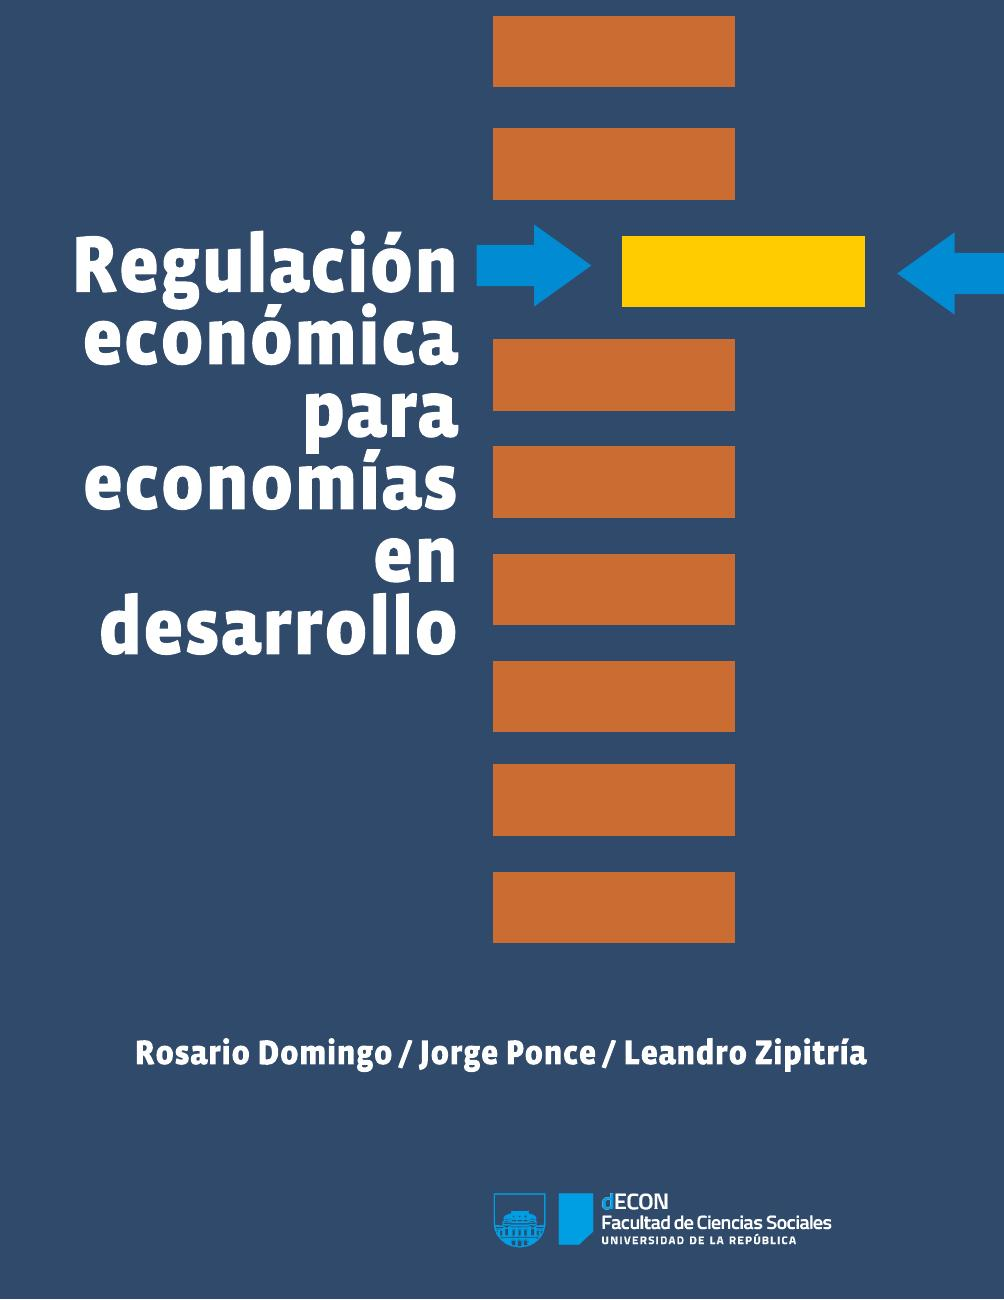
\includegraphics[width=6.64in,height=9.36in]{imagenes/cover.jpg} \end{figure} \pagebreak}
\usepackage[nottoc]{tocbibind}
\ifxetex
  % Load polyglossia as late as possible: uses bidi with RTL langages (e.g. Hebrew, Arabic)
  \usepackage{polyglossia}
  \setmainlanguage[]{spanish}
\else
  \usepackage[shorthands=off,main=spanish]{babel}
\fi
\usepackage[]{natbib}
\bibliographystyle{econometrica-es.bst}

\title{Regulación económica para economías en desarrollo}
\author{Rosario Domingo, Jorge Ponce, Leandro Zipitría}
\date{Esta version: 2020-03-31}

\begin{document}
\frontmatter
\maketitle

\mainmatter
\hypertarget{prefacio}{%
\chapter*{Prefacio}\label{prefacio}}
\addcontentsline{toc}{chapter}{Prefacio}

``Regulación Económica para Economías en Desarrollo'' por Rosario
Domingo, Jorge Ponce y Leandro Zipitría se distribuye bajo una Licencia
Creative Commons Atribución 4.0 Internacional
\href{http://creativecommons.org/licenses/by-nc-sa/4.0/}{Creative
Commons Attribution-NonCommercial-ShareAlike 4.0 International License}.

\textbf{Atribución} - Cite el trabajo de la siguiente forma: Domingo,
Rosario, Jorge Ponce y Leandro Zipitría (2016). Regulación económica
para economías en desarrollo. Departamento de Economía - FCS,
Universidad de la República, Montevideo.

ISBN: 978-9974-0-1325-4

Edición y corrección: Rosario Domingo.

Diseño de tapa: Rodolfo Fuentes / NAO

Los puntos de vista y las opiniones expresadas en esta publicación, son
responsabilidad de los autores y no necesariamente reflejan una posición
del Departamento de Economía de la Facultad de Ciencias Sociales de la
Universidad de la República.

\newpage

\hypertarget{intro}{%
\chapter*{Presentación}\label{intro}}
\addcontentsline{toc}{chapter}{Presentación}

La regulación por parte de los gobiernos es una de las características
principales de las economías modernas. Los mercados están sometidos a
distintas reglas que afectan su funcionamiento y el de las empresas que
en ellos actúan. A medida que las economías se desarrollan, las fallas
de mercado imponen restricciones al funcionamiento de la economía que
requieren ser atendidas, de forma de que puedan explotar todo su
potencial. Por tanto, conocer los instrumentos regulatorios disponibles
y entender cuáles son sus efectos sobre los mercados es clave para el
adecuado diseño de las políticas públicas. Asimismo, no sólo hay que
regular cuando es requerido, sino que hay que hacerlo de forma adecuada.

Este libro presenta los principales conceptos de la regulación económica
en forma simple, concisa y a la vez rigurosa. Su objetivo es que el
lector pueda familiarizarse con las herramientas regulatorias
rápidamente evitando, en la medida de lo posible, las discusiones
técnicas que subyacen los conceptos. Está dirigido a técnicos del sector
público con independencia de su formación profesional. Asimismo, está
escrito y diseñado con el objetivo de atender los problemas relevantes
de los países en vías de desarrollo y, en particular, los países
latinoamericanos. En él se describen los problemas que afectan a estos
países, cuyas instituciones regulatorias son muchas veces débiles para
enfrentar, de forma adecuada, la tarea de fomentar el funcionamiento de
los mercados.

El texto tiene su origen en el Diploma en Regulación Económica que se
dicta en la Universidad de la Habana, con el objetivo de formar técnicos
en las principales herramientas del análisis económico regulatorio. El
mismo se realiza y publica en el marco del programa de colaboración que
el Departamento de Economía de la UdelaR desarrolla con la Facultad de
Economía de la Universidad de la Habana, con el financiamiento de la
Agencia Sueca Internacional de Cooperación al Desarrollo (ASDI).
Asimismo, los dos últimos capítulos del libro están basados fuertemente
en un trabajo realizado por Domingo y Zipitría para la Unidad Reguladora
de los Servicios de Energía y Agua de Uruguay y que contó con
financiamiento de la Cooperación Andina de Fomento (CAF).

El capítulo @ref(reg-ec), escrito por Zipitría, introduce la temática de
la regulación económica. Discute la racionalidad económica de la
regulación y las distintas teorías que la explican. Se ilustra con
distintas regulaciones de la realidad de Uruguay y cómo éstas se
interpretan a la luz de las teorías descritas. Por último, desarrolla
las características de los mercados de monopolio natural en los cuales
se observa no sólo una importante regulación, sino también la presencia
de empresas públicas en distintos países en vías de desarrollo. Los
sectores de monopolio natural, en donde por razones tecnológicas
participa una única empresa del mercado, son sensibles desde el punto de
vista político debido a que sus productos son consumidos de forma masiva
y existen impor tantes costos hundidos. A la vez, en ellos no es posible
confiar en la competencia para que resuelva el funcionamiento eficiente
del mercado.

En el capítulo @ref(inst-reg), Zipitría introduce los principales
instrumentos regulatorios y sus efectos sobre el mercado. Si bien el
principal instrumento de evaluación del funcionamiento de los mercados
es la eficiencia, el capítulo no cuestiona otros fines que pueda tener
la regulación. Ello permite investigar los efectos, buscado y no
buscados, que la aplicación de los instrumentos regulatorios tiene sobre
el mercado. Muchas veces, en el diseño regulatorio, el énfasis se pone
en el efecto directo que el instrumento tiene sobre el comportamiento
que se busca modificar, cuando los efectos indirectos pueden alterar la
conducta de los agentes en los mercados en sentido no previsto y
empeorar el funcionamiento general del mismo. El análisis se realiza
identificando la forma de regulación óptima en cada estructura de
mercado ---competencia perfecta, oligopolio y monopolio natural--- y los
efectos que la misma tiene sobre su eficiencia.

El capítulo @ref(def-comp), del mismo autor, desarrolla los principales
conceptos del análisis de defensa de la competencia. En aquellos
mercados donde la competencia es factible, muchas veces las empresas
privadas buscan evitar que esta opere y reduzca las rentas que obtienen.
Por ello, se ha desarrollado un campo específico que intenta comprender
el funcionamiento de los mercados y el efecto de las conductas que los
agentes desarrollan. En la medida en que los países menos desarrollados
tienen dificultades para recopilar y acceder a información detallada de
la forma en la que operan los mercados, se presenta una discusión de los
instrumentos que permiten comprender su funcionamiento y tomar
decisiones fundamentadas sobre las acciones de los privados. Se
desarrolla el concepto de mercado relevante, que es el primer paso de
toda investigación de competencia, pero que es también una herramienta
general que puede ser útil para entender el funcionamiento de los
mercados. Posteriormente se analizan el abuso de posición dominante, la
colusión, las restricciones verticales y las fusiones de empresas que
son las conductas investigadas en esta materia. En cada caso, se expone
las razones económicas de los agentes para adoptar cada una de ellas,
así como sus efectos positivos y negativos sobre la eficiencia.

En el capítulo @ref(instituciones-reg), Ponce desarrolla una serie de
herramientas para el diseño de las instituciones regulatorias. La
regulación de los agentes privados en general, y en las economías en
desarrollo en particular, está sometida a una serie de problemas de
información, restricciones técnicas y presupuestales que hay que tomar
en consideración a la hora del diseño de dichas instituciones. En
particular, existe el riesgo de la captura del regulador por parte del
sector privado, un compromiso limitado y falta de credibilidad de los
reguladores, poca rendición de cuenta de sus acciones, baja eficiencia
para recaudar recursos fiscales que permita financiar las actividades
reguladas, corrupción y baja capacidad de hacer cumplir las normas.
Estos problemas alteran el diseño institucional óptimo de las agencias
encargadas de actuar sobre el sector privado y, si no son tenidos en
cuenta, pueden determinar que estos organismos se alejen en forma
relevante de los fines perseguidos.

En el capítulo @ref(reg-eepp), Domingo y Zipitría introducen la
regulación de las empresas públicas. A diferencia de los países
desarrollados, en los países en vías de desarrollo los Estados
participan en la actividad productiva en muchos sectores de la economía.
Las empresas públicas tienen características distintivas de las
privadas, que requieren considerarse a la hora de analizar su eficiencia
o su regulación. En particular, están fuertemente influenciadas por el
sistema político el cual les adjudica múltiples roles. Esta
multiplicidad de objetivos tiene impacto sobre le eficiencia del
funcionamiento de estas empresas, así como sobre la posibilidad de
evaluar el comportamiento y gestión de sus directores. Asimismo, algunas
veces las empresas públicas están sometidas a restricciones
presupuestales blandas, lo que afecta también en forma negativa su
eficiencia. Por otra parte, las restricciones que enfrentan sus
directores se traducen en mecanismos particulares de control de su
actuación, de forma de evitar que sean utilizadas con fines espúreos.

Por último, el capítulo @ref(eepp-uy) de los mismos autores presenta una
descripción de las empresas públicas en América Latina en general, y un
detalle de estas empresas y su regulación en Uruguay. El objetivo es
ilustrar con ejemplos concretos las múltiples dimensiones del análisis
de este tipo de empresas, así como la dinámica política a la cual están
sometidas. Asimismo, sirve para comprender los reveses que han
enfrentado los reguladores cuando tienen que regular a este tipo de
empresas.

Esperamos que este texto, por la presentación llana de los conceptos,
sirva de guía y de manual de referencia tanto para los participantes del
Diploma en Regulación Económica, como para los formuladores de
políticas.

Los autores.

\hypertarget{reg-ec}{%
\chapter{Regulación económica}\label{reg-ec}}

Leandro Zipitría

La esencia del funcionamiento libre del mercado es que a los agentes les
está permitido tomar sus propias decisiones \citep[357]{Viscusi2005}. En
términos generales, el mercado \footnote{Un mercado es el lugar donde se
  intercambian derechos de propiedad. Los derechos de propiedad incluyen
  cuatro derechos: (i) al uso; (ii) a obtener los retornos del bien;
  (iii) a transferir el bien; y (iv) a hacer cumplir los derechos de
  propiedad.} asigna en forma eficiente los recursos en mercados
perfectamente competitivos. Por ello, no existe motivo para intervenir
en los mercados, dado que las decisiones privadas de los agentes
coinciden con el bienestar social. Los mercados por sí solos resuelven
el problema de la asignación de recursos.

En algunos casos, sin embargo, el mercado no asigna en forma eficiente
los recursos y se producen \textbf{fallas de mercado}, las que pueden
ser de distinto tipo:

\begin{enumerate}
\def\labelenumi{\arabic{enumi}.}
\item
  \textbf{Externalidades}: refieren a costos o ingresos que los agentes
  no internalizan cuando toman una decisión. Una externalidad negativa
  se da, por ejemplo, cuando una empresa contamina un río y no considera
  los costos que acarrea limpiarlo o mejorar su proceso productivo para
  reducir la contaminación al elegir su nivel de producción. Una
  externalidad positiva ocurre cuando se crea conocimiento básico, ya
  que el científico o la institución financiadora no puede apropiarse
  completamente de los ingresos que este conocimiento genera. En ambos
  casos, los mercados no asignan en forma eficiente los recursos y
  tenderán a sobre (sub) producir si la externalidad es negativa
  (positiva).
\item
  \textbf{Bienes públicos}: son aquellos no excluibles (no se puede
  excluir a los agentes de su consumo) y no rivales (el consumo de una
  unidad del bien no disminuye la cantidad disponible para los demás
  consumidores). \footnote{Los bienes económicos tradicionales son
    excluibles y rivales.} Ejemplo de este tipo de bienes es el
  conocimiento, el aire o la defensa de una nación.
\item
  \textbf{Poder de mercado}: define la capacidad de una empresa o
  conjunto de empresas de fijar el precio de forma rentable por encima
  del nivel competitivo, conducta que conduce a pérdidas del bienestar
  social \citep[p.~8]{Carlton2004}. La existencia de poder de mercado
  determina mercados no competitivos. Este texto analiza la regulación
  de este tipo de falla de mercado.
\item
  \textbf{Asimetrías de información}: se da cuando las partes que
  intervienen en las transacciones no cuentan con la misma información
  sobre el producto, el servicio o el activo objeto de la transacción.
  Los problemas de asimetría de información impregnan las relaciones
  económicas entre agentes y puede hacer colapsar a los mercados. La
  idea clásica refiere a una situación en donde existen distintas
  calidades de bienes pero los demandantes no conocen la calidad
  específica que ofrece cada agente. En estas circunstancias, para
  determinadas valoraciones de compradores y vendedores, se puede
  demostrar que sólo serán transados los de peor calidad
  \citep[pp.~244-245]{Wolfstetter1999}. En el sector financiero y en la
  salud la asimetría de información es un problema relevante que
  determina que se necesiten instrumentos regulatorios específicos para
  mitigarla.
\end{enumerate}

En las economías modernas, los gobiernos en forma rutinaria toman
decisiones que buscan afectar la forma en la que los agentes económicos
se comportan y modificar tanto el bienestar de los mismos como el de la
sociedad. En particular, en su rol de reguladores, los gobiernos
restringen el conjunto de acciones disponibles para los agentes. Por
regulación se entiende las limitaciones impuestas a los agentes respecto
de la discreción de las decisiones que pueden tomar, materializadas a
través del uso de instrumentos legales y bajo la amenaza de alguna
sanción. Los gobiernos, a diferencia de los demás agentes sociales,
tienen el monopolio del poder de coerción, \footnote{Esta idea está
  basada en \citep{Weber1921}.} en particular, de hacer cumplir las
normas que ellos mismos dictan. \footnote{El lenguaje dice mucho de los
  pueblos; el idioma inglés tiene una palabra para ``hacer cumplir las
  normas'', enforcement, que el idioma español carece.}

Cuando se regula un mercado su resultado en términos de eficiencia
asignativa y productiva está co-determinado por las fuerzas del mercado
y el proceso administrativo. \footnote{No se consideran en este análisis
  elementos que refieren a si las normas son justas o éticas como
  justificación de la regulación, sólo si son eficientes desde el punto
  de vista económico. Para una discusión y crítica de esta visión, véase
  \citep[capítulo 3]{Baldwin2011}.} Las regulaciones pueden ser de
distinto tipo, y a los efectos de este texto se dividen en:

\begin{enumerate}
\def\labelenumi{\arabic{enumi}.}
\item
  \textbf{Económicas}: aquellas que afectan la eficiencia asignativa
  ---y productiva--- de los mercados, como ser la fijación de precios o
  cantidades, el número de competidores, la entrada o salida del
  mercado.
\item
  \textbf{Sociales}: incluyen las regulaciones medioambientales, las
  condiciones laborales, la protección del consumidor, y la seguridad de
  productos, entre otras. Entre ellas podemos encontrar las regulaciones
  que establecen requerimientos sobre la forma en la que se eliminan
  sustancias tóxicas en el ambiente, la información que deben tener los
  productos alimenticios o medicamentos sobre sus componentes, o los
  controles que se establecen sobre los lugares donde se venden los
  productos.
\end{enumerate}

No por ser las más importantes, sino porque es el eje central del texto,
nos vamos a concentrar en las regulaciones económicas. Sin embargo, las
regulaciones sociales también tienen justificación económica y deben ser
consideradas a la hora de formular las distintas políticas, ya que no
sólo son relevantes en sí mismas, sino que también tienen impactos sobre
las variables económicas. Las regulaciones económicas pueden, a su vez,
dividirse entre:

\begin{enumerate}
\def\labelenumi{\arabic{enumi}.}
\item
  \textbf{Regulaciones de estructura}: incluyen normas que alteran la
  estructura del mercado, como ser las que afectan la libre entrada y
  salida de empresas o agentes del mercado.
\item
  \textbf{Regulaciones de conducta o comportamiento}: afectan variables
  como el precio, la calidad de los productos, la cantidad que se transa
  en los mercados, la publicidad que pueden llevar a cabo las empresas,
  entre otros.
\end{enumerate}

En los últimos años ha surgido una importante literatura denominada
economía del comportamiento, que se encarga de analizar los
determinantes psicológicos de la conducta de los agentes, en particular
consumidores. La misma enfatiza que los individuos no son lo racionales
que la teoría económica sugiere, e impulsa regulaciones de
comportamiento que afectan la forma en la que los agentes procesan la
información que reciben y toman las decisiones, llamados ``empujones'' o
nudges en inglés. En la medida en que esta literatura está enfocada a
modificar la conducta de los demandantes, este texto no abordará la
regulación de comportamiento, la que se puede encontrar en textos como
\citep[ o \citet{Kanheman2015}]{Sunstein2009}.

La regulación es una las características distintivas de los Estados. Hay
normas generales relativas a: defensa de la competencia; defensa del
consumidor; quiebra de empresas; sociedades comerciales; habilitaciones
para locales comerciales e industriales; normas bromatológicas sobre la
calidad de los productos o procesos de producción de alimentos; entre
otras. También se dictan normas específicas o sectoriales, como las
vinculadas a: las telecomunicaciones; la banca; la energía eléctrica; el
transporte aéreo, terrestre y marítimo; los productos lácteos, cárnicos
y semillas; y un muy largo etcétera.

En Uruguay, los instrumentos regulatorios utilizados son, básicamente,
de dos tipos:

\begin{enumerate}
\def\labelenumi{\arabic{enumi}.}
\item
  Regulación de precios: se fija el precio de la leche fresca; el valor
  del taxi y del transporte urbano; las cuotas mutuales y el valor de
  los tiques moderadores en el sector de la salud; el precio de la
  energía eléctrica;\footnote{En este caso es tenue la línea que separa
    la regulación de la fijación de precios por parte de la empresa
    monopólica.} los precios máximos en el mercado del gas licuado de
  petróleo (GLP) y el de los combustibles, entre otros. \footnote{En
    América Latina en general, y en Uruguay en particular, las
    regulaciones de precio se basan en normas asociadas a las llamadas
    leyes de abastecimiento, que buscan regular directamente la oferta y
    el precio de los productos, sancionando penalmente el acaparamiento,
    entre otras prácticas. En Uruguay, se encuentra vigente la Ley
    No.~10.940 de setiembre de 1947 (sobre la base de la Ley No.~10.075
    de 1941 que regulaba los artículos de primera necesidad) que creó el
    Consejo Nacional de Subsistencias y Contralor de Precios. Esta norma
    permite, bajo ciertos parámetros, que el Poder Ejecutivo intervenga
    y fije el precio de los productos e intervenir empresas y secuestrar
    sus productos, bajo ciertos supuestos (artículo 13). En la
    actualidad, Venezuela cuenta con un control similar, a través de la
    Ley de Precios Justos, que fija el precio para los artículos de
    primera necesidad. En este caso los controles los realiza la
    Superintendencia de Precios Justos. También Argentina cuenta con
    leyes de este tipo desde 1974, con modificaciones introducidas en
    2010, véase la
    \href{http://infoleg.mecon.gov.ar/infolegInternet/anexos/55000-59999/58603/texact.htm}{ley
    No.~20.680}.}
\item
  Controles a la entrada y salida de los mercados: en el mercado
  bancario, operan importantes regulaciones ---prudenciales--- a la
  entrada y salida de bancos, que incluyen autorización previa por parte
  del Banco Central del Uruguay (BCU); en la telefonía celular, para
  entrar al mercado hay que acceder a una frecuencia que la otorga la
  Unidad Reguladora de los Servicios de Comunicaciones (URSEC); en la
  telefonía fija está prohibida la entrada a operadores del sector
  privado; en la habilitación a las farmacias, existe una ley que
  prohíbe que las mismas se instalen a menos de 300 metros de otra ya
  existente; en el establecimiento de cualquier emprendimiento de venta
  de productos alimenticios y de uso doméstico (supermercado) de más de
  200 metros cuadrados, la Ley de Protección de la Micro, Pequeña y
  Mediana Empresa Comercial y Artesanal, establece que se requiere
  consultar a una comisión asesora del Intendente municipal quien expide
  la autorización final; en la habilitación a carnicerías se requiere,
  entre otros, aprobación expresa del Instituto Nacional de Carne
  (INAC).
\end{enumerate}

Pero ¿cuál es la justificación de la regulación económica? \footnote{En
  esta temática se sigue fundamentalmente a \citet{Viscusi2005},
  capítulo 10; \citet{Hertog1999}; y \citet{Noll1989}.} En este capítulo
se presentan distintas explicaciones desde la ciencia económica, aunque
en la actualidad este campo también lo trata la ciencia política. La
primera justificación proviene de la teoría del interés público, que
establece que el gobierno actúa en forma benevolente para resolver
fallas de mercado.

La segunda se basa en la teoría de la captura regulatoria, en sus
distintas versiones, para la cual la regulación es un instrumento
utilizado por los grupos de poder para redistribuir renta a su favor. En
tercer lugar, se introduce una mirada que va más allá de las
particularidades del mercado en sí mismo y la regulación económica se
vincula a la interrelación entre el Estado y el sector privado y, en
particular, a la forma que tiene el Estado de controlar la convivencia
social. Por último, se realiza un detallado análisis de las
características de la regulación de monopolios naturales.

\hypertarget{la-teoruxeda-del-interuxe9s-puxfablico}{%
\section{La teoría del interés
público}\label{la-teoruxeda-del-interuxe9s-puxfablico}}

El principal fundamento para la intervención del gobierno en los
mercados se basa en la idea de que existen situaciones en las cuales los
mercados no conducen al máximo bienestar social, en particular, cuando
se producen fallas de mercado. Según esta teoría, la regulación persigue
el bienestar general cuando existen fallas de mercado y su objetivo es
corregirlas. El gobierno que diseña y ejecuta estas regulaciones lo hace
con espíritu benevolente, y no existen costos de transacción para
implementarlas. Antes de continuar, conviene discutir qué se entiende
por costos de transacción.

Este concepto tiene distintas definiciones, la más amplia de las cuales
establece que son los costos que se incurren para realizar un
intercambio económico. Los costos de transacción incluyen: (i) los
costos de búsqueda e información, es decir, determinar si el producto
está disponible en el mercado, cuál es su precio, quién lo tiene
disponible, etc.;(ii) los costos de negociación entre las partes para
alcanzar un acuerdo; y (iii) los costos de vigilar y hacer cumplir el
contrato refrendado entre las partes. Como puede apreciarse, en la
realidad es muy difícil encontrar situaciones en las cuales los costos
de transacción entre las partes sean cero.

Esta teoría recibe, al menos, dos críticas. La primera refiere a la
propia existencia de una potencial ganancia de eficiencia ---condición
necesaria para la regulación---, puesto que no explica cómo se logra
alcanzar esta ganancia a través de la intervención del gobierno. En
otros términos, cómo se pasa de una demanda pública a un resultado
concreto normativo con su consiguiente beneficio social.

En efecto, como señala \citet{Noll1989}, existen mecanismos alternativos
a la regulación como, por ejemplo, otorgar dinero a las familias de
menores recursos en lugar de fijar precios máximos a los bienes. Si ello
no es posible, es porque existen otras restricciones o los costos de
transacción no son cero. Sin embargo, no hay razón teórica para que los
problemas de información que enfrentan los privados, asociados a estos
costos de transacción, los puede superar el gobierno.

Asimismo, regular tiene costos. Estos están vinculados a la necesidad de
contratar una burocracia que analice el mercado y monitoree su
desempeño, así como a las ineficiencias que pueda generar la propia
regulación en el mercado (por ejemplo, menores incentivos al ingreso de
empresas si se limita el precio). Otras veces la regulación tiene una
inercia propia que dificulta el ajuste de la misma a los cambios en las
condiciones de mercado.

A vía de ejemplo, en Uruguay existe históricamente un precio máximo a la
leche fresca, producto del desabastecimiento que sufrió la ciudad de
Montevideo en la década del 30 \citep{Marti2013}. Aun cuando las
condiciones de mercado cambiaron sustancialmente, esta regulación se ha
mantenido casi por un siglo. \footnote{Dos problemas adicionales surgen
  en este análisis. En primer lugar, si por alguna consideración
  política esta regulación fuera necesaria, ¿qué bienes integran la
  canasta de productos de primera necesidad, cuyo monitoreo es
  necesario? En segundo lugar, ¿por qué se regula el precio de la leche,
  como artículo de primera necesidad, y no se regulan los otros
  productos que integran esta canasta como la harina o el pan? Las
  fallas de mercado no explican el porqué de esta regulación.} Asimismo,
no queda claro que el instrumento elegido (precio máximo) sirva como
solución al problema original (desabastecimiento).

La segunda crítica refiere a que se debería observar la regulación sólo
en aquellos sectores con fallas de mercado, lo que no siempre se cumple.
En muchos países se regulan mercados potencialmente competitivos como el
de transporte. En Estados Unidos (EUA) las críticas a este enfoque
fueron más fuertes. En la década de los 60, una serie de estudios
demostraron que la regulación, más que subsanar las fallas de mercado,
tendía a aumentar los beneficios de las industrias.

El problema radica en que el gobierno no está exento de la falta de
información, ni de los costos de transacción antes mencionados, por lo
que nada asegura que se puedan alcanzar los resultados óptimos a través
de la intervención estatal. Los procesos técnico-políticos que llevan a
la conformación de las decisiones gubernamentales son complejos y en
ellos, generalmente, intervienen muchos actores con intereses diversos.

Uno de los problemas fundamentales es que regular implica redistribuir
riqueza entre los agentes ---ya sea productores o consumidores--- y ello
lo convierte en un mecanismo muy atractivo para que los diversos actores
busquen participar en su diseño o implementación. \footnote{A vía de
  ejemplo, la Ley de Grandes Superficies que mencionáramos anteriormente
  tiene como objetivo explícito defender a la micro, pequeña y mediana
  empresa comercial y artesanal, uno de los miembros de la comisión
  asesora del Intendente es un representante de estos emprendimientos.}

\hypertarget{la-teoruxeda-de-la-captura-regulatoria}{%
\section{La teoría de la captura
regulatoria}\label{la-teoruxeda-de-la-captura-regulatoria}}

La evidencia empírica en EUA mostró que, hasta la década de los 60, la
regulación no estaba necesariamente correlacionada con las fallas de
mercado, sino todo lo contrario. Es decir, muchas regulaciones más que
resolver fallas de mercado estaban dirigidas a la protección de las
empresas instaladas. Ello llevó al desarrollo de la Teoría de la Captura
Regulatoria, la que sostiene que o bien la regulación se realiza en
respuesta a las demandas de la industria (los legisladores están
capturados por la industria) o las agencias regulatorias, con el paso
del tiempo, terminan siendo controladas por las industrias que deberían
regular.

\citet{Stigler1971} señala que la regulación es uno de los caminos que
tienen los grupos de interés para incrementar su bienestar, utilizando
al Estado para que redistribuya riqueza a su favor a costa de otros
grupos sociales. El Estado es un agente atractivo para redistribuir
riqueza debido a que dispone del poder de coerción. Por tanto, las
regulaciones a la entrada de los mercados, o las que imponen costos
excesivos o innecesarios a las nuevas empresas, son, según esta teoría,
el resultado de la captura del proceso económico por parte de los
instalados.

En Uruguay existen distintos ejemplos de normas que se ajustarían a esta
teoría. En primer lugar, la
\href{http://www.parlamento.gub.uy/leyes/AccesoTextoLey.asp?Ley=17715\&Anchor=}{Ley
No.~17.715} estableció una distancia mínima parael establecimiento de
nuevas farmacias respecto a las ya instaladas y, como resultado,
disminuye la competencia potencial de nuevos entrantes sobre los precios
de los instalados. En segundo lugar, las leyes
\href{http://www.parlamento.gub.uy/leyes/AccesoTextoLey.asp?Ley=17188\&Anchor=}{No.~17.188}
y
\href{http://www.parlamento.gub.uy/leyes/AccesoTextoLey.asp?Ley=17657\&Anchor=}{No.~17.657}
instauraron restricciones para el establecimiento de grandes superficies
(mayores a 200 metros cuadrados). Las mismas crearon una comisión
asesora al Intendente de cada departamento, que debe elaborar un informe
preceptivo ---pero no vinculante--- respecto de la conveniencia de la
instalación de nuevos supermercados, atendiendo a la demanda excedente,
la creación neta de empleos y la desaparición de establecimientos
tradicionales. Por último, en el sector de las telecomunicaciones se
observa en los últimos años un involucramiento relativamente laxo por
parte del órgano regulador (URSEC) a investigar y sancionar posibles
prácticas anticompetitivas que realice la empresa estatal ANTEL.

Sin embargo, tampoco es claro que toda la regulación sea el producto de
las acciones de los agentes ya instalados en los mercados, como lo
demuestra la existencia de subsidios cruzados entre consumidores. En
Uruguay, por ejemplo, la regulación fija precios únicos para algunos
bienes o servicios, lo que limita la capacidad de las empresas para
fijar precios. El ejemplo más claro es el del servicio de taxímetro en
el cual la tarifa está regulada (fija), lo que impide que las empresas
suban los precios en los momentos de mayor demanda.

Otras veces, este sesgo surge, más que en las normas en sí mismas, en su
aplicación. A las empresas grandes, a veces, se las controla de forma
más fuerte y efectiva que a las pequeñas, en el cumplimiento de las
normas. A vía de ejemplo, la empresa papelera UPM (ex BOTNIA) ha tenido
que cumplir con exigentes normativas para poder construir su planta y
existen distintos puntos de monitoreo, a lo largo del Río Uruguay, para
estudiar la calidad del agua. En el otro extremo, el control de la
contaminación de los ríos ha sido históricamente un objetivo de segundo
orden por parte de las autoridades departamentales \citep{Caffera2004}.
En efecto, la Intendencia Municipal de Montevideo ---al menos en el
pasado--- ha evitado sancionar a empresas que contaminan los ríos,
evitando su posible cierre, con el objetivo de proteger el empleo.

Entonces la pregunta parece ser ¿qué mercados serán los regulados?
\citet{Peltzman1976} desarrolla un enfoque teórico que presenta tres
componentes: (i) la regulación redistribuye riqueza; (ii) los
legisladores actúan guiados por el interés de mantener su puesto, lo que
implica que las normas que aprueban están diseñadas para maximizar el
apoyo político que reciben; (iii) los grupos de interés \footnote{Entendidos
  en sentido amplio: consumidores, empresas establecidas, competidoras,
  proveedores, trabajadores, etc.} compiten para ofrecer apoyo político
a cambio de una legislación favorable.

El resultado al que llega es que la regulación estará sesgada a favor de
aquellos grupos que estén mejor organizados o ganen más con una
legislación favorable, los que estarían más dispuestos a invertir
recursos para lograr el apoyo político a sus propuestas. Más
específicamente, la regulación beneficiará a pequeños grupos con
preferencias más homogéneas a costa de grandes grupos con preferencias
heterogéneas, en la medida en que las primeras tienen mayor facilidad
para alcanzar consensos relativamente estables entre sus componentes.

Tras estos argumentos está el efecto del parasitismo: grupos pequeños en
los cuales cada miembro tiene mucho para ganar con la legislación,
tienen más incentivos para apoyar políticamente la redacción, discusión
y aprobación de una ley. Por su parte, los grupos grandes ---en general
de consumidores--- están menos informados sobre el alcance de la
normativa e individualmente pierden poco, en relación con lo que gana
cada integrante del grupo que se beneficia con la regulación. A la vez,
los costos de oponerse a la iniciativa son altos y terminan beneficiando
a terceros que no incurren en dichos costos. En este sentido, los costos
de organizar grupos numerosos con intereses difusos, donde la acción que
pueda desplegar alguno de sus integrantes genera beneficios al resto de
los componentes del grupo, hace que sean más vulnerables a la hora de
oponerse a iniciativas de los grandes grupos empresariales.

\citet{Peltzman1976} presenta un modelo de fijación de precios por parte
de un legislador/regulador que busca maximizar el apoyo político. La
función de apoyo político es una función decreciente del precio (porque
los consumidores reducen el apoyo si el precio sube) y creciente en los
beneficios de la empresa. Por otro lado, los beneficios de las empresas
son crecientes en el precio, hasta que alcanzan el valor de monopolio.
En este modelo, el precio de equilibrio que elegirá el regulador es
aquél que maximice el apoyo político y, a la vez, esté sobre la frontera
de beneficios de las empresas. Por tanto, se cumple que el precio de
equilibrio estará entre el competitivo y el de monopolio. Como el precio
está entre los ``extremos'' se puede concluir que las industrias que
tenderán a estar reguladas son aquellas relativamente competitivas (a
demanda de las empresas) o aquellas relativamente monopolísticas (a
demanda de los consumidores).Según \citet{Viscusi2005} esta situación es
la que se observa en EUA, donde se regulan mercados monopólicos como la
telefonía local y de larga distancia, la transmisión de gas y
electricidad y los ferrocarriles; o sectores relativamente competitivos
como el transporte carretero, los taxis y la producción de energía o
gas.

En esta línea, \citet{Noll1989} presenta una vinculación interesante
entre la regulación y su retroalimentación con los grupos de interés. En
efecto, los sectores regulados, que generalmente obtienen beneficios
extraordinarios, construyen a su vez, dentro de las empresas, espacios
de negociación de las cuasi rentas obtenidas entre dueños y empleados.
Esto no sólo genera distorsiones en la asignación de recursos e
ineficiencias productivas (concepto que se desarrollará más adelante),
sino que genera resistencia por parte de los propios empleados a
modificaciones de las normas regulatorias. Esto es particularmente
interesante para Uruguay, donde la oposición a la desregulación de los
mercados de combustibles, telecomunicaciones o agua, provino
principalmente de los propios empleados de las empresas monopólicas, que
posteriormente volcaron a los consumidores a su favor.

Por último, \citet{Becker1983} sostiene que la regulación se da en un
contexto de competencia entre grupos de interés. La regulación, según
esta visión, es utilizada por aquellos grupos más poderosos para
incrementar su bienestar. En última instancia, todos los grupos de
interés generan alguna presión para intentar influir sobre las políticas
y, a la vez, tienen que vencer el problema del parasitismo. El modelo
que desarrolla Becker tiene algunos resultados de política.

En primer lugar, las políticas regulatorias que se implementarán serán
aquellas que mejoran la eficiencia, debido a que las ganancias que
obtienen los grupos de interés los inducirán a producir una mayor
presión para que se regule. En segundo lugar, y vinculado a lo anterior,
los sectores que tenderán a estar regulados son aquellos con más fallas
de mercado. Por último, no sólo se regularán los sectores con fallas de
mercado, sino también aquellos donde los grupos de interés sean más
eficientes para ejercer su presión. En otros términos, no sólo la
ganancia de eficiencia determina el resultado, sino la tecnología que
utilizan los grupos de presión para obtener su cometido.

\hypertarget{impuestos-a-travuxe9s-de-la-regulaciuxf3n}{%
\section{Impuestos a través de la
regulación}\label{impuestos-a-travuxe9s-de-la-regulaciuxf3n}}

La regulación no sólo es un instrumento para corregir fallas de mercado
o para que grupos de interés obtengan renta a su favor.
\citet{Posner1971} sostiene que los gobiernos utilizan la regulación
para redistribuir rentas entre consumidores, vía subsidios cruzados en
la venta de productos. Ello puede obedecer a distintos factores. Un
servicio donde es clásico el subsidio entre sectores es el transporte
urbano de pasajeros. Bajo este servicio, que en muchos países tiene
características de servicio público, se fija un único precio en todo el
transporte, lo que se transforma en un subsidio implícito desde los
recorridos de mayor demanda a los de menor demanda.

Como se verá en el capítulo @ref(inst-reg), ello tiene efectos sobre la
calidad del servicio, en la medida que, para que el mecanismo de
subsidio cruzado se pueda sostener, se requiere impedir la entrada a los
mercados más rentables, lo que en economía se conoce como el descreme de
los mercados. Al existir dos demandas, el precio debería ser menor en el
mercado donde la demanda es mayor, debido a que las posibilidades de
oferta serán también mayores y los consumidores tienen más oportunidades
de arbitraje, mientras que en los mercados con menor demanda habrá menos
oferentes y el precio será mayor.

En telefonía, este tipo de subsidio cruzado se le conoce como servicio
universal. Por ejemplo, en la telefonía fija, existe una tarifa única en
ciudades de alta y baja demanda, cuando el costo unitario de la red es
mucho más alto en las ciudades con menor densidad. En este caso, la
regulación de único precio ---unida a la restricción de entrada al
mercado, para evitar el descreme de los consumidores--- se utiliza como
un instrumento que sustituye a los impuestos, como mecanismo que permite
financiar las inversiones. En efecto, los altos costos asociados a la
telefonía serán difíciles de recaudar en mercados donde la densidad o
los ingresos son menores y, por tanto, un subsidio cruzado vía precio
permite que el gobierno realice inversiones en aquellos mercados donde
no tiene capacidad de recaudación, y que los consumidores con mayor
capacidad los subsidien.

Fijar impuestos a través de la regulación es una práctica factible
cuando la tecnología o las instituciones impositivas son débiles, ya sea
porque la base tributaria es pequeña, o porque son altos los costos de
recaudar, las distorsiones que conlleva la tributación o la evasión. En
cualquiera de estos casos, en lugar de fijar un impuesto, recaudarlo,
separar el dinero y pagar a la empresa, es más fácil y sencillo que la
propia empresa cobre el dinero directamente a través del precio. Ello
genera los incentivos adecuados a la empresa para cobrar por el
producto. Sin embargo, por otro lado, esta regulación genera barreras a
la entrada al mercado que luego son difíciles de alterar.

\hypertarget{regulaciuxf3n-y-cumplimiento-de-las-normas}{%
\section{Regulación y cumplimiento de las
normas}\label{regulaciuxf3n-y-cumplimiento-de-las-normas}}

Las teorías anteriores presentan una visión de la regulación como un
instrumento en sí mismo, aislado de otros disponibles por los gobiernos
para controlar el accionar de las empresas en los mercados. Sin embargo,
\citet{Djankov2003} y \citet{Shleifer2005} presenta una visión diferente
de la regulación. Sostienen que si la sociedad quiere, por alguna razón,
controlar a las empresas privadas dispone de cuatro estrategias
diferentes, las que presentan una tensión entre los poderes del Estado y
las libertades individuales. Esta tensión, en última instancia, se
refleja en que a menor intervención del Estado, mayores son las pérdidas
sociales debidas a la expropiación privada (la denominan desorden),
mientras que a mayor intervención del Estado mayores son las pérdidas
debido a la expropiación del Estado (la denominan dictadura). Si el
Estado se retira de la vida privada, los agentes quedan a merced del
desorden, pero se minimizan los riesgos de dictadura, mientras que al
aumentar la participación del Estado se reduce el desorden, pero
aumentan los riesgos de dictadura. En otros términos, los agentes
privados pueden expropiarse unos a otros, pero el Estado también puede
expropiar a los privados. \footnote{Esta visión está muy vinculada a las
  ideas de los derechos de propiedad. Para que estos puedan ejercerse se
  requiere un Estado que los haga cumplir. Sin embargo, si el Estado no
  tiene contrapesos, también puede apropiarse de los derechos de los
  privados.}

Los cuatro instrumentos de que dispone una sociedad para controlar al
sector privado son: (i) la disciplina de mercado; (ii) los litigios
judiciales entre privados; (iii) la regulación; y (iv) la propiedad
pública. Estas estrategias no son mutuamente excluyentes, dado que en
muchas sociedades conviven entre sí. En Uruguay, por ejemplo, existe
propiedad pública en el sector de telecomunicaciones, el que a su vez
está regulado por un órgano regulador específico, los privados pueden
llevar a juicio civil a la empresa pública y, en última instancia,
pueden dejar de comprarle. El uso creciente de los instrumentos
regulatorios balancea la forma en que la sociedad pondera los riesgos
asociados al desorden y la dictadura. La clave es que, a medida que se
hace más complejo para la sociedad controlar al sector privado
(desorden), se comienza a recorrer un arco de posibilidades que implican
una mayor intervención del Estado.

¿Por qué distintas sociedades resuelven un mismo problema de forma
diferente? Esta pregunta no tiene una única respuesta. Las capacidades
institucionales para regular de los países difieren entre sí. Se
observan diferencias en relación con lo que las normas permiten hacer a
los reguladores, la capacidad sancionatoria, el grado de tecnificación
de la burocracia y la permeabilidad del sistema político a las presiones
del sector privado. Asimismo, lo que algunas sociedades toleran que se
resuelva a través del Sistema Judicial, otras requieren de una
intervención directa del Estado \citep{Alesina2005}. Lo interesante de
este enfoque es que permite comprender en forma amplia la existencia de
regulación y empresas públicas. Hay teorías que abordan el tema de las
empresas públicas como un asunto político \citep{Shleifer1994}, donde
los políticos utilizan a las empresas públicas para mantenerse en el
poder. Sin embargo, \citet{Shleifer2005} presenta una visión que
fundamenta la existencia de empresas públicas como una solución
eficiente desde el punto de vista institucional: dadas las restricciones
que enfrentan los Estados, el avance en una dirección regulatoria
representa la mejor solución posible para controlar el desorden.

\hypertarget{la-regulaciuxf3n-de-monopolios-naturales}{%
\section{La regulación de monopolios
naturales}\label{la-regulaciuxf3n-de-monopolios-naturales}}

Esta sección se centra fundamentalmente en estudiar la regulación de
aquellos sectores que no están sometidos a competencia debido a que es
eficiente que la producción la lleve a cabo una única empresa. En
algunos sectores de la economía ---en particular en transmisión de
energía, agua potable, saneamiento, vías férreas, o transmisión de
datos--- la tecnología de producción de bienes y servicios se
caracteriza por la existencia de importantes inversiones fijas y
hundidas. \footnote{Las inversiones hundidas son aquellas que una vez
  realizadas no pueden asignarse a otros usos más allá de los previstos
  originalmente.}

Ello determina que la provisión de ciertos servicios públicos sea
eficiente si la realiza un número limitado de oferentes y, en algunos
casos, sólo si lo hace una única empresa. La necesidad de contar con
activos fijos que tienen un costo muy importante y que en sí mismos
permiten atender a toda la demanda, implica que la duplicación de esta
infraestructura sea ineficiente desde el punto de vista económico. Uno
de los supuestos que explica la existencia de mercados competitivos es
que las empresas que en ellos operan tienen un tamaño tal que con una
infraestructura dada no pueden atender a toda la demanda. \footnote{Los
  supuestos se completan con la libre entrada y salida de los mercados,
  la perfecta homogeneidad de los bienes, la ausencia de costos de
  transacción, información perfecta por parte de los agentes y, en el
  largo plazo, igual acceso a la tecnología de producción.} Ello permite
que varias empresas puedan coexistir para atender el mercado. Por su
parte, cuando es eficiente que una única empresa atienda a todo el
mercado se entiende que existe un monopolio natural. \footnote{Para un
  desarrollo sencillo de la teoría de monopolio natural ver
  \citet{Viscusi2005}, capítulo 11.}

Para avanzar en este concepto, hay que considerar que la eficiencia
económica es un fenómeno que tiene múltiples dimensiones. \footnote{En
  \citet{Viscusi2005}, capítulo 4, se presenta una exposición del
  concepto de eficiencia. Para un desarrollo en profundidad ver
  \citet{Motta2004}, capítulo 2.} Eficiencia refiere a la forma en la
que se utilizan los recursos para obtener un determinado nivel de
producción. Sin embargo, este concepto tiene dos dimensiones según si la
mirada es de corto o largo plazo. En el corto plazo, esto es cuando se
considera un mercado o tecnología de producción dada, se define la
\textbf{eficiencia estática}.

Por su parte, \textbf{la eficiencia dinámica} es un concepto de largo
plazo que refiere a la forma en la que se introducen nuevos productos o
nuevos procesos de producción. A vía de ejemplo, cuando se habla de
eficiencia en el mercado de la telefonía fija se está analizando la
eficiencia estática del sector, el producto está dado y la tecnología de
producción también. Por su parte, cuando se estudia la introducción de
fibra óptica al mercado de transmisión de datos, dado que éste es un
producto nuevo que crea un mercado con características diferentes a los
existentes ---permite brindar más servicios que la tecnología
tradicional---, se analiza la eficiencia dinámica.

Este último tipo de eficiencia, implica estudiar los incentivos que
tienen los agentes para llevar a cabo actividades de investigación y
desarrollo (I+D) que permitan introducir nuevos procesos productivos o
desarrollar nuevos productos. La clave está en el proceso por el cual se
generan nuevos mercados, sea de productos o procesos de producción. La
eficiencia dinámica es esencial en aquellos mercados, como el de las
telecomunicaciones, donde la norma es la introducción permanente de
nuevas tecnologías. Estas nuevas tecnologías pueden provocar cambios en
los mercados existentes y hacer que muchos de ellos desaparezcan o se
transformen en forma radical en períodos breves.

A su vez, el énfasis en cada tipo de eficiencia tiene asociada una
visión diferente de la competencia. Cuando se analiza la eficiencia
estática se está estudiando la competencia \textbf{en el mercado},
mientras que si se analiza la eficiencia dinámica el énfasis está en la
competencia \textbf{por el mercado}. Las competencias en y por el
mercado tienen lógicas diferentes aunque en ambas subyace la misma
noción de empresas compitiendo entre sí. \footnote{La importancia de la
  competencia en el desarrollo económico ha sido desarrollada por
  \citet{Aghion2005}.}

La eficiencia estática se centra en comprender cómo compiten las
empresas y cómo utilizan sus recursos productivos en un mercado dado con
una tecnología de producción específica; y tiene dos miradas:

\begin{enumerate}
\def\labelenumi{\arabic{enumi}.}
\item
  \textbf{eficiencia asignativa} que refiere al excedente o bienestar
  económico que genera una determinada estructura de mercado. Un mercado
  competitivo genera un excedente mayor que una estructura monopólica
  debido a que el monopolio tiene incentivos a restringir la oferta, de
  forma de aumentar el precio de mercado y sus beneficios. Por tanto, el
  monopolio genera una ineficiencia asignativa o pérdida de eficiencia
  asignativa.
\item
  \textbf{eficiencia productiva} que analiza la forma en la que se
  utilizan los insumos para generar un nivel de producto dado. La clave
  es determinar si existe derroche de recursos. Este análisis tiene a su
  vez dos niveles. Por un lado, si existen diversas tecnologías
  disponibles, cuál es la que permite obtener un nivel dado de producto
  al menor costo posible. Por otro lado, para un nivel dado de
  tecnología, si la misma se utiliza en todo su potencial. En el
  análisis de la eficiencia productiva surgen diversos factores que
  determinan que una empresa sea ineficiente. Puede ser el resultado de
  una mala elección de la tecnología, por ejemplo vender servicios de
  transmisión de datos utilizando un par trenzado (cable de cobre) en
  vez de fibra óptica; \footnote{Véase
    \url{http://es.wikipedia.org/wiki/Medio_de_transmisi\%C3\%B3n\#Medios_de_transmisi.C3.B3n_guiados}}
  o puede ser el resultado de utilizar fibra óptica pero llegar a pocos
  clientes y, por tanto, que el servicio sea muy costoso.
\end{enumerate}

La clave en el análisis de la eficiencia productiva está en que la
elección de la tecnología y su uso dependen de los incentivos que
enfrenten las empresas \citep{Nickell1997}. En general, la competencia
en el mercado se transforma en un incentivo suficiente para que las
empresas utilicen la mejor tecnología disponible y la usen al máximo de
su potencial, ya que de otra forma corren el riesgo de quebrar.
\footnote{Véase \citet{Motta2004}, sección 2.3.2.} En estos casos la
competencia se transforma en un mecanismo de selección de tipo
darwinista en el cual sólo sobreviven las empresas más eficientes. Otras
veces, la forma de propiedad sirve como incentivo al uso eficiente de
los recursos. Si la empresa cotiza sus acciones en la Bolsa y es
ineficiente, entonces obtendrá menores beneficios de los potenciales y,
por ello, corre el riesgo de perder valor para sus accionistas. Por lo
tanto, es más probable que sus gerentes sean despedidos, mecanismo que
tienen los accionistas para proteger su inversión. \footnote{\citet{Laffont1993}
  señalan que las empresas públicas pueden también sufrir el relevo de
  sus directivos, o del propio gobierno, pero las causas son generales
  -no dependen del funcionamiento específico de la empresa- y los
  incentivos de los políticos a mirar el resultado de la empresa son
  menores a los de los inversores.}

La existencia de un monopolio natural en determinados mercados, se
explica por la eficiencia productiva. Cuando resulta eficiente que la
producción del bien o servicio se realice en una única empresa ---los
costos de producción son menores respecto a fragmentar la producción en
varias firmas---, entonces existe un monopolio natural. Es claro que
esta característica de la función de costos depende, también, de la
forma de la demanda. Cuanto menor sea la demanda más factible es que la
inversión realizada por una única empresa alcance para atenderla. En
Uruguay, una única planta de refinamiento de petróleo es suficiente para
abastecer a todo el mercado interno, lo que resultaría imposible en el
caso de Argentina, que cuenta con unas diez refinerías de petróleo.

Cuando es eficiente que una única empresa sirva al mercado (eficiencia
productiva), esta única empresa, si maximiza beneficios, se comportará
como un monopolista. A menor competencia en el mercado, donde el
monopolio es la expresión extrema, más restringirán las empresas su
producción de forma tal que los productos resulten escasos y los
consumidores paguen precios mayores por los mismos.

Por tanto, estos mercados conllevan un compromiso entre eficiencias que
tienen direcciones opuestas: por un lado, la eficiencia productiva
---costos--- favorece la existencia de una única empresa en el mercado;
por otro, la eficiencia asignativa ---poder de mercado--- implica que
surja el riesgo de abuso de posición de dominio por parte del único
oferente. La forma en la que los Estados han resuelto este compromiso es
permitir la existencia de una única empresa, pero regular su precio para
evitar abusos. Este balance explica el surgimiento de la regulación por
parte del Estado.

Los servicios públicos, generalmente, se encuentra en mercados donde al
menos un componente de la actividad constituye un monopolio natural.
Estos servicios se caracterizan por: (i) un alto monto y especificidad
de los activos involucrados; (ii) la existencia de economías de escala o
de variedad; y (iii) el consumo masivo de muchos de los bienes y
servicios que producen. Las \textbf{economías de escala} implican que
los costos unitarios de producción decrecen a medida que la producción
se expande, mientras que las \textbf{economías de variedad} indican que
la producción conjunta de determinados bienes presenta costos menores
que si se producen en forma separada \citep{Bergara2003}. Ambas
economías explican la existencia de monopolios naturales.

Asimismo, en la provisión de muchos servicios públicos se observa
sectores de onopolio natural que conviven con segmentos potencialmente
competitivos. Por ejemplo, el servicio de electricidad tiene distintos
componentes: generación, transmisión y distribución. Mientras la
transmisión eléctrica es un ejemplo típico de monopolio natural, tanto
la generación como la distribución son segmentos donde puede operar la
competencia. \footnote{Una descripción detallada del sector eléctrico se
  puede encontrar en \citet{Viscusi2005},capítulo 12.} Por su parte, la
fibra óptica ---que tiene características de monopolio natural--- es un
insumo necesario para actividades que se desarrollan en mercados que
pueden ser competitivos como la transmisión de datos, ya sea telefonía,
internet o televisión para abonados. \footnote{No hay estudio para
  Uruguay que concluya que la fibra óptica sea un monopolio natural,
  aunque existen pistas de que si podría serlo en muchos mercados
  geográficos.}

A modo de resumen, en el Tabla @ref(tab:cuadro1) se presentan los
principales tipos de eficiencia y su impacto sobre la estructura de
mercado.

\begin{longtable}[]{@{}lllll@{}}
\caption{Tipos de eficiencia, características e impacto sobre
estructuras de mercado.}\tabularnewline
\toprule
Tipo de eficiencia & Tipo de competencia & Categorías & Características
& Efecto de la competencia\tabularnewline
\midrule
\endfirsthead
\toprule
Tipo de eficiencia & Tipo de competencia & Categorías & Características
& Efecto de la competencia\tabularnewline
\midrule
\endhead
Estática & En el mercado & Asignativa & Asociada a poder de mercado &
Mejora la eficiencia\tabularnewline
Estática & En el mercado & Productiva & Asociada a la tecnología &
Resultado ambiguo\tabularnewline
Dinámica & Por el mercado & Dinámica & Asociada a la innovación & Ex
ante, induce la innovación\tabularnewline
\bottomrule
\end{longtable}

Fuente: elaboración propia.

La regulación surge como un mecanismo para controlar los incentivos que
tienen las empresas monopólicas a cobrar precios abusivos a los
consumidores, es decir resolver una falla de mercado. Como resultado de
la misma, el mercado se suplanta por un mecanismo burocrático que define
varias de las variables relevantes: el precio, la calidad de los
productos, o las inversiones que puede o no realizar la empresa. La
regulación no es una solución perfecta, en la medida en que los
reguladores tienen en general menos información que la empresa regulada
y ello puede impedir alcanzar resultados de primer óptimo. \footnote{El
  resultado de primer óptimo es el que se obtendría si el regulador
  tuviera el mismo nivel de información que la empresa. Si ello no es
  así, entonces ese resultado no se puede implementar, y se deben
  establecer valores de las variables que induzcan a las empresas a
  revelar su información y a reducir, en la medida de lo posible, las
  distorsiones de eficiencia.} Sin embargo, es aceptado que en el caso
de los monopolios naturales es preferible un mecanismo que concentre la
producción en una empresa ---eficiencia productiva--- y que regule las
demás variables relevantes para evitar el abuso vía precio ---eficiencia
asignativa.

La regulación tiene en sí misma complejos problemas de implementación:
¿cuál es la discrecionalidad óptima del regulador?; ¿cómo se debe fijar
y revisar las tarifas?; ¿qué costos deben considerarse?; ¿cuál es la
tasa de retorno adecuada de los proyectos?; ¿qué mínimos de calidad se
deben exigir a las empresas?; ¿qué justificaciones se aceptan para los
apartamientos?; ¿se prevé la expropiación de la empresa o no?; ¿se puede
introducir nueva competencia en mercados relacionados? Todos estos
elementos determinan la forma en la que se diseñan las instituciones
regulatorias e involucran un fino balance entre flexibilidad y
expropiación \citep{Bergara2003, Spiller2013}. \footnote{La regulación
  de servicios públicos, por su naturaleza, presenta dificultades a la
  hora de fijar reglas claras y hacerlas cumplir, siendo el marco
  institucional que delimita estas actividades un ingrediente clave para
  alcanzar los objetivos regulatorios \citep{Bergara2003}.}

Por otra parte, el órgano regulador dispone de diversos instrumentos a
los efectos de evaluar y sancionar a las empresas que no cumplan con las
regulaciones establecidas. En primer lugar, partiendo del paradigma
tradicional regulatorio, donde las empresas tienen como objetivo
claramente establecido maximizar los beneficios que obtienen por
realizar la actividad productiva \citep{Armstrong2007}, un instrumento
sencillo, a los efectos de alinear los objetivos de las empresas a los
del regulador en las variables relevantes, es la aplicación de sanciones
pecuniarias. Toda vez que la empresa incumpla con los términos del
servicio, el regulador impone una sanción que reduce los beneficios de
la empresa. Si la sanción es mayor al beneficio que obtiene la empresa
por no cumplir con los objetivos impuestos por el regulador, entonces,
evitará incurrir en estos comportamientos. \footnote{Véase
  \citep{Becker1968}}

Un segundo elemento que incide en el comportamiento de las empresas
privadas es su reputación. Si la empresa cotiza en Bolsa, esto es,
obtiene su financiamiento a través del mercado de capitales, cualquier
sanción que efectúe el regulador tendrá no sólo el efecto directo sobre
los beneficios de la empresa, sino también sobre el valor de las
acciones para sus titulares, lo que impacta en las decisiones que
adoptan los gerentes.

Un tercer elemento, que recoge la historia de las empresas públicas en
Uruguay, refiere a la amenaza de estatizar los servicios públicos. En
efecto, si la calidad de los servicios prestados es deficiente, o si la
empresa incumple lo establecidoen el contrato de concesión, entonces
existe la posibilidad de que el Estado asuma la responsabilidad de la
prestación del servicio, desplazando a la empresa privada. En la medida
en que los servicios públicos tienen características de monopolio
natural y el Estado es el responsable de que los mismos se brinden en
forma adecuada a sus ciudadanos, si fallan los instrumentos regulatorios
para alcanzar este objetivo, entonces el Estado debe hacerse cargo del
servicio en cuestión. En estos tres casos, la regulación puede incidir
sobre el accionar de la empresa privada a través de las sanciones
económicas.

Asimismo, la provisión de servicios públicos por parte de empresas
privadas implica alguna relación contractual entre el gobierno y la
empresa proveedora. Esta relación puede establecerse a través de una
concesión, una licencia, una autorización, u otra figura jurídica. En
general, estos contratos establecen los objetivos generales de la tarea
que debe realizar la empresa como operador, y el rol regulador y
planificador del gobierno.

Sin embargo, la lógica regulatoria es diferente en el caso de empresas
públicas. Estas empresas pueden perseguir objetivos distintos a la
eficiencia y, por tanto, la regulación de empresas privadas y públicas
encuentra límites diferentes. Sin embargo, la regulación de empresas
públicas se encuentra con políticas cuya aplicación puede ser discutible
y, por tanto, los instrumentos regulatorios tradicionales no pueden
aplicarse en esos casos.

\hypertarget{conclusiones}{%
\section{Conclusiones}\label{conclusiones}}

La regulación es uno de los instrumentos con los que cuentan los Estados
para intervenir en los mercados. Las regulaciones pueden obedecer a
factores económicos o sociales. Si bien su origen ha estado vinculado a
las fallas de mercado, también puede deberse a problemas
redistributivos. \footnote{Es decir, las fallas de mercado no son
  condición necesaria ni suficiente para la regulación.} Las teorías
queexplican la regulación van desde una visión optimista del Estado, en
términos de su accionar desinteresado para resolver los problemas del
mercado, hasta hipótesis que explican la regulación como el resultado de
un proceso de captura por parte de la industria para obtener rentas.

En cualquier caso, la regulación es un proceso complejo
\citep{Dixit1998}. Involucra el diseño de una institución reguladora,
dotarla con fondos necesarios para llevar a cabo su tarea y con
funcionarios capacitados para cumplir sus objetivos. Sus cometidos
requieren un adecuado balance para que las instituciones sean efectivas.
Por un lado, tienen que estar diseñados de forma lo suficientemente
amplia para atender los problemas que motivaron su creación, evitando el
arbitraje regulatorio por el cual las empresas eluden controles si
pueden realizar acciones que no están reguladas, pero que generan los
mismos efectos sobre el mercado que las que sí lo están . Por otro,
estos controles deben ser lo suficientemente específicos para evitar que
los reguladores se extralimiten en sus tareas o persigan otros intereses
a los previstos.

No debe olvidarse que los reguladores, por más bien intencionados que
puedan estar y aunque dispongan de recursos adecuados, contarán siempre
con menos información que las empresas que deben regular. Ello determina
que siempre estén un paso atrás de las empresas. Asimismo, como se verá
en el capítulo @ref(inst-reg), la decisión de regular un mercado afecta
a un conjunto de variables y ello debe ser considerado a la hora del
diseño regulatorio. Muchas veces fijar una variable altera los
incentivos de los agentes y tiene impacto sobre otras de ellas, lo que
puede más que compensar el efecto positivo original de la regulación.
\footnote{Un típico ejemplo son los precios máximos en mercados
  competitivos, que generan escasez.} Por último, cuando el Estado
regula será responsable, tanto de los buenos como de los malos
resultados del mercado. La regulación genera siempre efectos sobre la
eficiencia de los mercados.

\hypertarget{inst-reg}{%
\chapter{Instrumentos regulatorios}\label{inst-reg}}

Leandro Zipitría

Este capítulo presenta los principales instrumentos regulatorios y sus
efectos en los mercados. Si el objetivo es estudiar los problemas
regulatorios que surgen con motivo del poder de mercado de las empresas,
el principal instrumento regulatorio que considera la literatura es el
precio. Sin embargo, la efectividad de este instrumento para corregir
los problemas detectados en el mercado dependerá de las características
del primero, de la estructura del segundo, y del objetivo planteado por
la regulación.

En general, los problemas que busca resolver la regulación son de
eficiencia económica, ya que se presupone que para los asuntos
distributivos existen otros instrumentos disponibles. No obstante,
muchas veces los Estados intervienen sobre los mercados con el objetivo
de resolver problemas distributivos, y es importante conocer los efectos
que estos instrumentos tendrán sobre el mercado. Asimismo, en ciertas
situaciones el precio no es suficiente para resolver el problema bajo
análisis y debe ser complementado con otros instrumentos. Este capítulo
presenta los principales instrumentos regulatorios y sus efectos en los
mercados.

Si bien en gran parte de este capítulo se trabajará como si el regulador
pudiera conocer las variables relevantes de la o las empresas que
pretende regular, en la gran mayoría de los casos este desconoce el
funcionamiento del mercado y de las empresas que en él operan. Esta
asimetría de información es muy difícil de resolver, ya que implica
diseñar instrumentos que permitan a las empresas revelar las variables
que el regulador desconoce.

Sin embargo, este acto de revelación nunca es desinteresado o altruista,
sino que se inscribe en un marco estratégico de las empresas con vistas
a influir en la regulación. Para que las empresas revelen la información
que disponen, deben tener incentivos, lo que implica costos para el
regulador. Por ello, el gobierno en general, y los reguladores en
particular, conocerán en forma relativamente indirectael funcionamiento
de los mercados y siempre estarán menos informados que las empresas. En
otros términos, a veces se señala que la regulación viene rezagada
respecto a las acciones del mercado, producto de estas asimetrías de
información.

Los instrumentos regulatorios son diversos. \footnote{En el capítulo
  @ref(def-comp) se realiza una descripción de un conjunto de
  instrumentos que se utilizan para analizar los mercados y fomentar la
  competencia.} Unos instrumentos fijan o limitan algunas de las
variables del mercado y, por tanto, restringen las acciones de las
empresas. El precio es la principal variable regulatoria y su
determinación, por parte del regulador, influye sobre los beneficios de
las empresas y, con ello, sobre otras acciones que estas pueden llevar a
cabo. Precio no sólo refiere al valor de un bien o servicio, sino
también al momento o valor por el que se incrementa.

El regulador, también, puede establecer restricciones para el ingreso al
mercado, limitando o simplemente impidiendo el ingreso de nuevas
empresas, o puede establecer restricciones a la salida de empresas del
mercado, aun cuando estas tengan pérdidas por vender sus bienes en el
mercado. Estas dos restricciones, al ingreso y a la salida, se utilizan,
por ejemplo, cuando se regula el transporte público, e implica impedir
que una empresa abandone una determinada frecuencia aun cuando esta sea
deficitaria (restricción a la salida), o en otros casos impedir el
ingreso a frecuencias con mayor demanda (restricción de entrada). Otro
instrumento que puede utilizar el regulador es someter a su control o
aprobación la realización de determinadas inversiones por parte de las
empresas, como la incorporación de determinadas tecnologías, y, en
algunos casos, puede obligar a las empresas a invertir en ciertos
activos específicos.

Existen diversas formas de presentar los instrumentos regulatorios. Se
puede analizar cada instrumento (precio, entrada y salida, calidad,
etc.) y determinar el efecto que tiene en los distintos mercados.
Alternativamente, se puede analizar cada estructura de mercado y
estudiar el efecto que los distintos tipos de intervenciones tienen
sobre su desempeño. Esta última alternativa es la que se seguirá en este
capítulo, lo que permitirá tener una visión integral del funcionamiento
de los instrumentos regulatorios y de los efectos de la regulación,
tanto deseados como no deseados. Asimismo, se vincularán los
instrumentos regulatorios con otros que se analizarán en capítulos
siguientes, como la defensa de la competencia.

Aunque parezca evidente, lo primero que hay que tener claro cuando se
piensa en regular un mercado es el por qué. En principio, los
economistas sostieneque la regulación es necesaria para resolver algún
tipo de falla de mercado. Sin embargo, muchas veces la regulación existe
por inercia o tradición; \footnote{El caso más claro en Uruguay es el de
  la leche fresca, cuyo precio máximo se encuentra regulado desde hace
  décadas.} o porque se persiguen otros fines, como distributivos o
asegurar la prestación de un servicio; \footnote{El transporte público,
  a vía de ejemplo.} o porque se busca atender otras fallas de mercado,
como se analizó en el capítulo @ref(reg-ec). La regulación, también,
surge por demanda de los actores en los mercados. Una vez que se ha
resuelto regular ---y se sabe por qué---, el siguiente paso es
determinar el instrumento adecuado que resuelve el problema
identificado. Luego se requiere establecer una infraestructura que
permita fijar el instrumento elegido y monitorear el desempeño del
mercado. Idealmente, habría que realizar evaluaciones para analizar el
funcionamiento del instrumento aplicado, aunque, en la práctica, esto se
hace con poca frecuencia. \footnote{Además de los propios regulados, que
  muchas veces defienden la regulación, también los reguladores estarán
  interesados en mantenerla. Una vez que el mecanismo ha sido puesto en
  marcha, es difícil desactivarlo.}

En términos ideales, cualquier regulación que impacte sobre el mercado
debería contar con un análisis costo-beneficio, y sólo deberían ser
aprobadas aquellas cuyos beneficios superen a los costos. En Europa o
Inglaterra, existen lineamientos de evaluación de impacto regulatorio,
que apuntan a la \textbf{mejor regulación}, en oposición a menor
regulación. \footnote{Véase \citet{UE2015} y \citet{BRE2015}} Sin
embargo, en los últimos años la evaluación costo-beneficio ha cambiado
su foco hacia una evaluación de políticas, que es un campo mucho más
amplio que el que se analiza aquí. \footnote{El lector interesado puede
  ver una aproximación amigable a estas técnicas en \citet{Gertler2011}}
Mientras la evaluación costo-beneficio se centra en las regulaciones que
afectan la competencia en los mercados, la evaluación de políticas es un
instrumento mucho más amplio para determinar la efectividad de las
políticas públicas, incluidas las regulaciones de mercado.

En la siguiente sección se analiza la regulación de mercados
competitivos, mientras que en la segunda sección se analizan los
mercados oligopólicos. En la tercera sección se analizan los
instrumentos regulatorios en los mercados de monopolios naturales. Al
final, se presentan algunas reflexiones sobre el impacto del uso de los
instrumentos regulatorios en los mercados.

\hypertarget{regulaciuxf3n-de-mercados-competitivos}{%
\section{Regulación de mercados
competitivos}\label{regulaciuxf3n-de-mercados-competitivos}}

El juego de mercado ---la interacción entre oferta y demanda--- arroja
un resultado de equilibrio en términos de precios y cantidades
transadas. Si el mercado es perfectamente competitivo, se obtienen
algunos resultados deseables desde el punto de vista económico.
\footnote{El adjetivo deseable hace referencia a la eficiencia del
  resultado, no a si el mismo es justo o equitativo, cualquiera sea la
  forma en la que se definan.} Para avanzar en los efectos de la
regulación sobre estos mercados, primero hay que entender cuáles son sus
características y evaluar su desempeño. \footnote{Esta sección y la
  siguiente están basadas en \citet{Viscusi2005}, capítulo 16.}

¿Qué caracteriza a un mercado perfectamente competitivo? Los supuestos
tradicionales incluyen: (i) atomicidad de oferentes y demandantes; (ii)
perfecta homogeneidad del producto; (iii) información perfecta de todos
los participantes respecto al precio, ubicación y stock de los
productores y productos; (iv) igual acceso a la tecnología de
producción, que impide que alguna empresa tenga una ventaja sobre las
restantes; y (v) libre entrada y salida del mercado. Básicamente, estos
supuestos permiten que los consumidores arbitren a los productores,
estos últimos estén en igualdad de condiciones unos con otros y puedan
aprovechar las oportunidades que el mercado les provee.

En estos mercados, las empresas actúan como tomadores de precio ya que
cualquier intento por aumentarlo inducirá a los consumidores a arbitrar
a los vendedores. Salvo en los mercados donde hay rendimientos
crecientes a escala en la producción ---un elemento que incide en la
existencia de un monopolio natural--- en el resto de los mercados es
factible encontrar equilibrios competitivos. Los rendimientos crecientes
a escala son una propiedad de la función de producción ---aquella que
permite transformar insumos en productos--- y que determina que los
costos promedio de producción disminuyan al aumentar el volumen
producido.

La atomicidad es un supuesto de importancia menor, con relación a los
otros supuestos. La Teoría de los Mercados Disputables, pone el énfasis
en la competencia potencial de los posibles entrantes, respecto a la
competencia efectiva en los mercados. Si bien esta teoría requiere de
supuestos relativamente fuertes ---como la ausencia de costos hundidos
en el mercado y la homogeneidad del producto--- pone sobre el tapete la
importancia de la amenaza a la entrada como mecanismo que disciplina a
las empresas establecidas. \footnote{Los costos hundidos son aquellos
  que no se recuperan si la empresa quiere salir del mercado.} Si la
competencia potencial es lo suficientemente fuerte, no es necesario que
el mercado esté atomizado para obtener los resultados de competencia
perfecta.

El equilibrio de competencia perfecta tiene algunas propiedades
deseables. En primer lugar, es la estructura con el menor precio
relativo, ya que cualquier estructura alternativa ---oligopolio o
monopolio--- implica que las empresas tendrán un cierto grado de poder
de mercado. En segundo lugar, y como corolario del anterior, la cantidad
transada en ese mercado será la mayor posible. En tercer lugar, los
consumidores obtendrán el mayor excedente posible, en la medida en que
se cumplen los dos primeros puntos. Desde el punto de vista del
consumidor, no hay situación de mercado más beneficiosa que la
competencia.

En economía, el \textbf{excedente del consumidor} es la diferencia entre
lo que este está dispuesto a pagar por el producto y lo que
efectivamente paga en el mercado. En competencia perfecta, como el
precio de todos los bienes es el menor posible, la cantidad de bienes
será la mayor posible y el excedente del consumidor será máximo. En
cuarto lugar, las empresas producen al menor costo posible, ya que la
producción se realiza en el punto donde los costos medios son mínimos.
Esta condición técnica se alcanza debido a que el ingreso de nuevas
empresas al mercado llevará la producción individual al punto en el cual
se minimizan los costos. Por último, en competencia perfecta las
empresas realizan un beneficio económico cero en el largo plazo. Desde
el punto de vista de la eficiencia, el resultado de competencia perfecta
es deseable.

Si la competencia en el mercado no es suficiente, lo que provoca precios
altos, entonces existe una serie de pasos previos a la regulación. En
primer lugar, actuar sobre las posibles barreras o regulaciones
estatales que dificulten el ingreso de empresas al mercado e impidan el
ajuste competitivo. En segundo lugar, si estas barreras son producto del
accionar de las empresas, impulsar acciones de defensa de la
competencia, siguiendo el análisis que se realiza en el capítulo
@ref(def-comp).

Sin embargo, puede suceder que el Estado quiera regular un mercado
competitivo, a pesar de sus beneficios, fijando directamente el precio
del producto. Ello tendrá un impacto negativo sobre el bienestar, ya sea
porque los precios aumentan, o porque se genera escasez. A continuación
se presentan distintos escenarios donde un regulador actúa sobre alguna
variable en un mercado competitivo.

En un primer escenario, supongamos que el regulador fija un precio por
debajo del precio competitivo. Ello tiene diversos impactos sobre el
mercado. En primer lugar, dado que el precio es menor al de equilibrio,
la oferta a ese precio será menor a la demanda y, por tanto, habrá
escasez de productos. Un ejemplo de esta situación, lo observamos hoy en
Venezuela, donde los precios de los productos están fijados
administrativamente considerando márgenes de ganancia ``adecuados''.
Como estos precios no reflejan la escasez relativa de los productos, se
genera una escasez de productos básicos que es creciente con la
distancia entre el precio fijado y el precio de equilibrio. \footnote{Sobre
  los márgenes en Venezuela, véase el artículo 5o de la
  \href{http://www.superintendenciadepreciosjustos.gob.ve/sites/default/files/PROVIDENCIA\%20070-2015.pdf}{Providencia
  Administrativa No.~070/2015}. Sobre la escasez en Venezuela, véase la
  información en
  Wikipedia:\href{https://es.wikipedia.org/wiki/Escasez_en_Venezuela}{``Escasez
  en Venezuela''}}

En segundo lugar, y asociado a este efecto, los consumidores tenderán a
sobre utilizar o sobre demandar el producto, ya que la baja en el precio
expande la demanda. Esta sobre demanda surge porque el precio no refleja
el equilibrio de mercado ni las posibilidades de los oferentes. Ello
tiene un efecto que debe ser considerado cuando se regulan algunos
servicios públicos como el transporte, ya que si el precio es muy bajo,
no habrá capacidad que soporte la demanda. Si, por otra parte, el precio
se fija por encima del competitivo, se produce el efecto inverso, ya que
la demanda cae y la oferta es excesiva.

En cualquier escenario, regular un mercado competitivo lleva a una
pérdida de eficiencia con relación a no regularlo. Pero si la decisión
es la de fijar un precio ---máximo o mínimo---, entonces es mejor
complementarlo con restricciones a la salida o entrada al mercado.

En un segundo escenario, supongamos que se regula fijando un precio
mínimo (máximo) por encima (debajo) del competitivo y operan
restricciones a la entrada (salida) al mercado. En este caso, nuevas
empresas querrán entrar (salir) del mercado, debido a que existe una
renta positiva (negativa). Sin embargo, como la demanda cae (aumenta)
las empresas producirán por debajo (encima) del punto donde los costos
medios son mínimos, lo que en cualquier caso aumenta su costo de
producción. En definitiva, restringir la entrada (salida) del mercado,
permite que las empresas mejoren la eficiencia productiva, al disminuir
sus costos de producción respecto a una situación en la cual existe
libre entrada y salida.

Sin embargo, si bien es fácil exponer estos mecanismos, es mucho más
complejo en la realidad poder encontrar los puntos donde oferta es igual
a demanda y manejar un número de oferentes en el mercado. No debe
olvidarse que mientras las empresas reciben directamente los efectos de
sus acciones, los reguladores en cambio sólo perciben estos efectos en
forma indirecta.

Ambas regulaciones (fijación de precio y restricción de entrada/salida)
tienen impactos sobre los incentivos de los agentes, que alteran otras
variables competitivas. En el caso en que se fija un precio máximo y se
limita la entrada, se producen al menos dos efectos. En primer lugar, al
establecerse el precio del producto las empresas recurrirán a otros
mecanismos para competir. En particular, buscarán diferenciarse por
calidad u otros atributos del producto, de forma de atraer a la demanda.
Ello a la vez genera un problema dinámico, ya que las empresas tenderán
a aumentar la calidad más allá de lo que prevalecería en un mercado sin
regulación de precio, lo que, a su vez, determina que estas empresas no
podrán sobrevivir si se elimina la regulación, ya que deberán competir
con empresas cuya calidad será menor.

En otros términos, la sobre inversión en calidad es una respuesta de los
agentes a la regulación de precio. Esta posibilidad de que las empresas
inviertan en calidad surge siempre que las empresas no puedan coludir
entre sí. Si lo hacen, entonces pueden evitar realizar estas inversiones
y simplemente repartirse la renta extra. Esta posibilidad lleva al
segundo efecto, ya que la restricción de entrada afecta los incentivos
de las empresas a controlar la ineficiencia productiva. En efecto,
cuando la amenaza de la competencia es laxa, las empresas tienden a
relajar sus controles sobre los costos, lo que incrementa la
ineficiencia productiva.

Muchas veces, como se vio en el capítulo @ref(reg-ec), las empresas
buscan generar una demanda por regulación y reparten renta con sus
empleados, de forma de generar grupos de interés más fuertes para
sostener las restricciones (y la renta). A la vez, este aislamiento
relativo que enfrentan las empresas determina que el mecanismo
darwinista de selección falla, y las empresas ineficientes no salen del
mercado ya que están protegidas por el precio alto y la regulación de
entrada.

En el caso en que la regulación establece precios por debajo de los
competitivos, y se incluye una restricción a la salida (o una
obligatoriedad de brindar el producto), nuevamente encontramos dos
efectos. Por un lado, si el precio no reconoce el retorno al empresario,
o si directamente no cubre los costos, pero existe una obligación de
vender el producto, entonces se verá afectada su calidad.

En Uruguay, ello pasaba con el pan tarifado, que era un pan que las
panaderías estaban obligadas a ofertar a un precio determinado. En caso
de no contar con este producto, debían sustituirlo por otro de mayor
calidad. En los hechos, el precio que se fijaba por el producto apenas
cubría el costo de la harina para producirlo, con el consiguiente
impacto sobre la calidad del mismo. Por otra parte, esta regulación
afecta la inversión en formación de capital de la empresa. Si el precio
de mercado no cubre los costos de reposición del capital, entonces las
empresas dejarán de invertir y, en algunos casos, hasta de mantener las
inversiones realizadas, con el consiguiente deterioro sobre la
eficiencia.

Otro escenario posible es cuando el regulador establece subsidios
cruzados, afectando a más de un mercado al mismo tiempo. Si existen dos
mercados con demandas y costos diferentes, pero se fija un único precio
que es a la vez mínimo en un mercado y máximo en el otro, entonces el
regulador estará fijando esquemas de subsidios entre mercados. Un
resultado paradójico de este tipo de políticas es que ningún consumidor
estará satisfecho. Los consumidores que pagan el producto más caro, no
estarán satisfechos sabiendo que la entrada de más empresas implicaría
mejores precios, mientras que aquellos que lo pagan más barato, en
general, encuentran restricciones de oferta dado el precio que
enfrentan. Una práctica más eficiente de fijación de precio, que se verá
en la sección \ref(monop-nat), es establecer una política de precios de
Ramsey. En los hechos esta política implica fijar precios en cada
mercado atendiendo a la demanda en cada uno de ellos.

En Uruguay, el transporte terrestre de pasajeros tiene este tipo de
políticas. El Poder Ejecutivo fija una tarifa por kilómetro recorrido,
independientemente del destino. Asimismo, se asigna a dos empresas las
frecuencias entre dos ciudades y también se reparten los destinos entre
las empresas, de forma que tengan destinos rentables y otros poco
rentables. Por tanto, existe un subsidio cruzado entre los destinos con
un precio fijado independientemente de la demanda y restricciones a la
entrada y salida de los mercados.

\hypertarget{mercados-oligopuxf3licos}{%
\section{Mercados oligopólicos}\label{mercados-oligopuxf3licos}}

Si bien los mercados perfectamente competitivos tienen características
económicas deseables, los mismos son la excepción, principalmente en
economías pequeñas. Pero aun cuando los mercados no sean perfectamente
competitivos, puede haber competencia entre oferentes aunque su número
sea reducido. Si esto ocurre, entonces el mercado es un oligopolio.

A diferencia de los mercados de competencia perfecta, las empresas en
oligopolio enfrentan una demanda con pendiente negativa. En los mercados
perfectamente competitivos se suponía que cada empresa tenía un tamaño
tal que no podía atender a todo el mercado y, por tanto, las empresas
eran tomadoras de precio. Por ello, se enfrenten a una demanda
perfectamente elástica al precio de mercado: precios mayores sacarán a
la empresa del mercado, precios menores arrojarán beneficios menores a
mantener el precio, o aún negativos. Sin embargo, cuando hay pocas
empresas en el mercado cada una tiene cierto grado de poder de mercado
y, por tanto, cualquier aumento que fije en el precio provocará una
caída de su demanda que pasará a sus competidores. La demanda que
enfrenta cada empresa tiene una relación inversa con el precio que fija.

Existen múltiples razones por las cuales los mercados no funcionan en
forma perfectamente competitiva. En primer lugar, los bienes
difícilmente son homogéneos. Todas las empresas buscan diferenciar sus
productos a través de la publicidad, presentación o estrategias de
marketing. Asimismo, aun cuando los bienes sean homogéneos, como la
gasolina, los puntos de venta pueden estar ubicados a distancias que
hacen que los consumidores los perciban como productos diferentes. Los
mismos productos vendidos en dos tiendas en dos barrios diferentes serán
productos distintos para el consumidor, toda vez que el costo de
trasladarse de un lugar a otro haga inútil el esfuerzo de arbitrar a los
productores. Este concepto está vinculado al de mercado relevante
geográfico que se analiza en el capítulo @ref(def-comp).

En segundo lugar, en muchos mercados existen barreras a la entrada y, en
particular, costos hundidos que desalientan el ingreso de nuevas
empresas. Como se señala en el capítulo @ref(def-comp), los costos
hundidos son muy importantes a la hora de considerar el ingreso a un
mercado. Ejemplos de estos costos son la capacitación de personal, la
publicidad, la inversión en la construcción de una marca o la
instalación de activos específicos ---maquinaria--- para realizar una
determinada actividad. Cuanto más específicos sean los activos, menos
líquidos serán en caso de que el emprendimiento fracase, lo que
incrementa los riesgos de entrar al mercado.

En tercer lugar, los consumidores no están perfectamente informados ni
sobre las tiendas que venden los productos, ni sobre los precios que
ellas fijan. Esta asimetría de información permite a las tiendas cobrar
precios superiores a aquellos consumidores que tienen un costo de
búsqueda mayor, ya sea porque tienen menos tiempo para informarse o una
menor utilidad por hacerlo. Este desconocimiento, además, incrementa los
costos de entrar al mercado ya que las empresas tienen que hacer conocer
a los consumidores ---y, a veces, hasta a los propios comercios--- sus
productos.

Un cuarto elemento es tecnológico. Las empresas tienen un tamaño de
escala (escala mínima eficiente), que es la que define el nivel mínimo
de producción eficiente para la empresa. Si existen economías de escala,
definida como aquella situación en la cual los costos medios disminuyen
a medida que aumenta la producción, entonces un mercado soportará un
número acotado de productores. Si, además, la demanda del producto es
relativamente acotada, entonces un mercado no podrá soportar un gran
número de empresas, a menos que esté dispuesto a tolerar altas
ineficiencias productivas, en términos de duplicación de activos fijos.
Por tanto, el tamaño del mercado pone un límite al número de empresas
que pueden operar en él.

Si hay un número limitado de oferentes, los beneficios que obtendrán
serán el decisiones de las firmas. Toda vez que una empresa fije una
variable (precio, calidad, ubicación geográfica, publicidad, capacidad,
etc.) ello tendrá impacto sobre los restantes oferentes, que a su vez
reaccionarán. A diferencia de los mercados competitivos, donde la única
variable de decisión es la cantidad producida y ella no genera reacción
de los demás oferentes, en un oligopolio las decisiones de las empresas
estarán vinculadas entre sí.

El oligopolio presenta diferencias importantes respecto a la competencia
perfecta. A los efectos de la regulación, la diferencia principal es que
en competencia perfecta la libre entrada a los mercados conduce a un
resultado eficiente (menores precios, mayor cantidad, menores costos),
mientras que en oligopolio la libre entrada produce sobre o sub ingreso
al mercado \citep{Mankiw1986}.

El exceso de ingreso al mercado se produce por el efecto \textbf{robo de
negocio}, en el cual la empresa entrante observa el beneficio que podría
obtener al ingresar, que está compuesto por beneficios genuinos que se
generan en el mercado pero también por aquellos que quita a las empresas
instaladas. Como a la sociedad sólo le importa los primeros (nuevos
beneficios que se generan por el ingreso de la firma), puesto que los
segundos (los que se apropia de empresas instaladas) constituyen un tema
redistributivo, los incentivos a entrar al mercado son más fuertes de lo
óptimo. Por tanto, entran demasiadas empresas al mercado. Este exceso de
ingreso se produce, fundamentalmente, en mercados donde los bienes son
relativamente homogéneos. En el caso de que los bienes sean
diferenciados, la entrada de nuevas empresas al mercado genera un nuevo
beneficio para los consumidores que se suma a la reducción en el precio,
y es que aumenta la variedad de productos disponibles.

En este caso, como los productores no internalizan este efecto que
producen sobre los consumidores, se puede producir una entrada menor a
la óptima en el mercado. En realidad los productores tienen incentivos
al ingreso, producto del efecto robo de negocio, pero aun así la entrada
puede ser ineficiente.

Por tanto, según el paradigma con el que se evalúan las regulaciones en
este texto ---la eficiencia--- existirían razones para regular la
entrada en mercados oligopólicos. Sin embargo, regular mercados
oligopólicos presenta múltiples problemas. El primero, es saber cuál es
el número óptimo de empresas en el mercado, tarea que es muy compleja
debido a las fuertes asimetrías de información entre el regulador y las
empresas que participan o podrían participar en el mercado. Además, hay
que saber si el problema es de ingreso excesivo o insuficiente.

En segundo lugar, el anuncio de una política regulatoria en estos
mercados dispararía acciones por parte de los interesados de forma de
manipular el proceso regulatorio a su favor, en los términos discutidos
en el capítulo @ref(reg-ec), que fomentaría la captura regulatoria. Ello
es muy factible si se consideran las asimetrías de información señaladas
anteriormente.

En tercer lugar, la libre entrada es un buen antídoto contra la
ineficiencia productiva. Las empresas, si no están sometidas a la
competencia, tienden a relajarse, disminuir la calidad de sus productos
o reducir la innovación, en la medida en que no enfrentan la amenaza de
dejar el mercado. Por todos estos problemas, es mejor soportar cierto
grado de ineficiencia en la entrada de empresas, que crear una oficina
para regular el número óptimo de ellas.

\hypertarget{monop-nat}{%
\section{Monopolios naturales}\label{monop-nat}}

En principio, todos los monopolios naturales deberían estar regulados.
\footnote{Esta sección se basa en \citet{Viscusi2005} y
  \citet{Joskow2007}.} Desde el punto de vista de la eficiencia, el
balance entre eficiencia productiva y asignativa establece que la
prioridad sea la primera, mientras la segunda se controle a través de la
regulación. Sin embargo, existen monopolios naturales con distintas
características. Por ejemplo, carreteras, aeropuertos, puertos u otras
obras de infraestructura tienen características de monopolio natural. Un
\textbf{monopolio natural} opera cuando es más barato ---menos
costoso--- producir un conjunto de bienes dentro de una empresa que
dividir la producción entre distintas empresas. Es decir, es más barato
atender la demanda del mercado a través de una única empresa. Esta
situación se da por una condición técnica de la función de costos, la
subaditividad.

El monopolio natural puede ocurrir en la producción de uno o más
productos. Cuando se analiza un único producto, una de las fuentes
principales que influyen en el surgimiento de un monopolio natural, es
la existencia de \textbf{economías de escala}. Muchos mercados utilizan
tecnologías en las que operan economías de escala, como el gas por
cañería, el agua potable o el saneamiento. Todos ellos tienen un
elemento en común: existen importantes inversiones fijas y hundidas. Por
ello, es eficiente que una única empresa abastezca al mercado, ya que
duplicar la inversión fija aumenta los costos de llevar el servicio a
cada uno de los hogares.

Las economías de escala son una condición suficiente, pero no necesaria
para la existencia de un monopolio natural. En los hechos, puede ser que
los costos medios sean crecientes para una demanda dada, pero permitir
el ingreso de una nueva empresa y duplicar los activos fijos provoca que
los costos medios se disparen por encima del incremento que se
observaría con una única empresa, de forma que conviene mantener la
producción en una única empresa.

Cuando las empresas producen más de un producto, entonces el análisis es
similar, pero hay que agregar una nueva dimensión al análisis: los
costos de producción pueden disminuir cuando se produce conjuntamente
más de un bien. Esta característica técnica se conoce como
\textbf{economías de alcance o variedad}, las que surgen por la
presencia de un activo o insumo común a la producción de los distintos
bienes.

Por ejemplo, el petróleo es un insumo que permite obtener gas, gasolinas
y asfalto, lo que determina que existan economías de alcance en la
producción conjunta de los bienes. La generación de energía eléctrica
utiliza un único activo ya sea para generar electricidad para consumo
residencial o industrial, que son dos demandas ---productos---
diferentes. Un único aeropuerto permite brindar servicios de pasajeros y
carga, mientras que algo similar ocurre con las carreteras. Sin embargo,
cuando las empresas producen más de un bien, para que exista un
monopolio natural se requiere la existencia simultánea de economías de
alcance y de escala. \footnote{En realidad, se cumple cuando existen
  economías de alcance y costos medios decrecientes a lo largo de un
  rayo, que es una forma de economía de escala. La referencia clásica
  del análisis de monopolios naturales es \citet{Panzar1989}}

\hypertarget{regulaciuxf3n-ex-ante}{%
\subsection{\texorpdfstring{Regulación \emph{ex
ante}}{Regulación ex ante}}\label{regulaciuxf3n-ex-ante}}

Un primer mecanismo para regular los monopolios naturales es sustituir
la competencia ex post por la competencia ex ante. Esta teoría fue
desarrollada por \citet{Demsetz1968} como una reacción a la regulación
de precio de los servicios públicos. La idea es sencilla e implica
fomentar la competencia entre oferentes en la etapa previa a la
concesión de un bien o servicio. Si existe un número suficiente de
empresas interesadas en desarrollar una actividad, construir un puerto o
una carretera, entonces se puede licitar para adjudicar el monopolio a
la empresa que oferte el precio más bajo por el servicio, dado un nivel
de calidad mínimo.

Este tipo de procedimiento se puede utilizar para algunos servicios. La
licitación resulta un instrumento adecuado, por ejemplo, para la
construcción y mantenimiento de una carretera, un puerto o un
aeropuerto. Este instrumento requiere establecer de antemano todas las
variables relevantes (calidad del servicio e inversiones y su
mantenimiento) mientras dure el período de concesión, lo que es factible
sólo en algunos casos. En última instancia, se debe restringir el número
de variables de decisión, de forma que se pueda asignar la licitación
sobre la base de criterios objetivos establecidos \emph{ex ante}.

Una forma de hacerlo es incluyendo un proceso en dos etapas en la
licitación, en la primera se seleccionan las ofertas en términos de la
calidad del proyecto, y una vez seleccionados los que pasan el nivel
mínimo establecido se procede a la elección del ganador por precio. Si
no es posible establecer de antemano todas las variables relevantes para
llevar a cabo el proyecto, debido, entre otros, a que existe
incertidumbre sobre algunas variables del mercado, utilizar el
procedimiento licitatorio puede llevar a renegociar el contrato durante
la vigencia de la concesión. Si la empresa tiene una costosa inversión
hundida, renegociar un contrato la pone en una posición débil para hacer
valer sus intereses. \footnote{Ver \citet{Bergara2003} capítulo 2, o
  \citet{Williamson1998}.} En estos casos la credibilidad del gobierno
para atarse de manos, esto es evitar expropiar a la empresa, pasa a ser
el elemento determinante en el juego regulatorio.

Por otra parte, para que las inversiones en estos mercados se realicen,
los plazos por los que se concesiona el servicio tienen que ser lo
suficientemente extensos para que los inversores puedan recuperar la
inversión a un precio razonable para el consumidor. Durante la vigencia
de la concesión, tienen que existir reglas claras y creíbles para que el
inversor tenga incentivos a invertir en los activos necesarios. Cuanta
mayor seguridad exista respecto al procedimiento licitatorio y a la
ejecución del posterior contrato de concesión, mayor número de oferentes
habrá inicialmente, y menores tasas de retorno exigirán al proyecto. La
clave es, por tanto, el diseño de los pliegos de la licitación.

\hypertarget{regulaciuxf3n-de-precio}{%
\subsection{Regulación de precio}\label{regulaciuxf3n-de-precio}}

El problema del monopolio es que fija precios excesivos respecto a los
que prevalecerían en mercados más competitivos. Por tanto, se puede
fijar un precio máximo en los mercados donde opera un monopolio natural.
En principio supondremos que el regulador tiene a disposición toda la
información relevante sobre el mercado y la empresa. En este marco,
puede elegir los valores de precio que sean adecuados para minimizar la
pérdida de eficiencia asignativa.

Si la empresa produce un único producto, el regulador podría replicar el
resultado de competencia perfecta y fijar el precio igual al costo
marginal, o sea al costo de producir la última unidad. Sin embargo, en
los mercados de monopolio natural este tipo de estrategia impedirá que
la empresa pueda cubrir sus costos fijos, ya que debido a la existencia
de economías de escala, los costos medios son menores a los marginales
en el tramo relevante donde se fijaría el precio. \footnote{Esto no
  ocurre en un mercado competitivo, donde la regla de fijar el precio
  igual al costo de la última unidad producida permite recuperar los
  costos fijos.}

En general, este problema se puede resolver si se subsidia a la empresa
los costos fijos. Sin embargo, ello es bastante difícil de implementar
en términos políticos (subsidiar a un monopolio no parece una idea
fácilmente defendible) y además los gobiernos, muchas veces, no cuentan
con los recursos para pagar estos costos directamente. Por tanto, una
alternativa es fijar el precio igual al costo medio y con ello generar
recursos para sostener los costos fijos.

Otra alternativa posible es establecer una tarifa en dos partes, en vez
de fijar un precio único. \textbf{Las tarifas en dos partes} involucran
un pago fijo y luego un pago variable por unidad consumida. El pago fijo
puede ser una tarifa de acceso, o un pago fijo mensual por el servicio.
Algunas veces permite consumir un número fijo de unidades, otras veces
es sólo un pago sin contrapartida.

Por ejemplo, la empresa de telefonía fija en Uruguay tiene un cargo fijo
de cómputos y luego un cargo variable, a partir de un determinado número
de unidades, mientras que la empresa de gas tiene un cargo fijo de
metros cúbicos de gas y luego un cargo variable. En ambos casos, el
esquema fijo se paga aún si no se consume o si se está por debajo del
umbral establecido, mientras que si se supera el umbral se paga por
unidad adicional. Lo interesante de este esquema es que se puede
utilizar el pago fijo para recuperar los costos fijos y el precio para
cubrir los costos variables. Esta alternativa es más eficiente, ya que
fijar un precio igual al costo medio tiene implícita una ineficiencia
asignativa, en la medida en que el precio que regiría es mayor al costo
marginal. Con la tarifa en dos partes esta ineficiencia desaparece.

Las tarifas en dos partes son un tipo de tarifa no lineal, a través de
la cual el precio varía según el consumo del agente. Otro tipo de tarifa
no lineal es cuando se cobra distintas tarifas según el consumo del
agente, en donde se fija un precio para las primeras \(X\) unidades
consumidas, otro precio \(Y\) a partir de la unidad \(X+1\), y así
sucesivamente. Este tipo de tarifa no lineal es la que se utiliza en
Uruguay en el sector de agua potable. El precio del metro cúbico de agua
consumida varía según el tramo de consumo y, en particular, es creciente
con el consumo mensual. \footnote{Ver
  \href{http://www.ose.com.uy/descargas/clientes/tarifas/ose_decreto_tarifario_2019.pdf}{tarifas
  de OSE}.} Este tipo de tarifa busca desincentivar el uso excesivo de
agua potable, penalizando a los consumidores que la utilizan para
finesrecreativos.

Otro elemento a considerar en el caso de los servicios públicos ---dada
la sensibilidad política de estas actividades--- es que muchas veces los
precios fijados no reflejan el valor de los servicios sino que se
implementan subsidios cruzados entre distintos sectores. Asimismo, el
hecho de que opere una única empresa en el mercado genera incentivos a
relajar el esfuerzo, dado que los consumidores están cautivos.

Por ello, no basta con determinar el precio en un marco de monopolio. El
regulador debe establecer también mínimos de la calidad del servicio,
dado que el monopolista tiene incentivos a utilizar la calidad del
servicio para discriminar a los consumidores y aumentar sus beneficios.
En efecto, dado un nivel de precio, si el monopolista puede elegir la
calidad de los servicios entonces tenderá a ampliar la brecha entre la
menor y mayor calidad. De esta forma, se discrimina a los consumidores
con más disposición a pagar vía la compra del servicio de mejor calidad
pero más caro. \footnote{Ver \citet{Belleflamme2015}, sección 9.2.1.}

En la práctica, los órganos reguladores disponen de un conjunto mayor de
instrumentos \citep{Berg2013}. Los mismos pueden agruparse en aquellos
que son sustantivos para el cumplimiento de sus cometidos, y aquellos
que son auxiliares y sirven para cumplir en forma adecuada con los
primeros. Entre los instrumentos sustantivos que disponen los
reguladores, además de fijar el precio del servicio, también se
encuentran: (i) la emisión de las licencias que permiten operar en los
mercados regulados (regulación de la entrada); y (ii) el establecimiento
de los estándares de calidad del servicio (regulación de la calidad).

Por otra parte, es necesario que el regulador disponga de herramientas
de apoyo para cumplir con sus cometidos fundamentales, en forma
adecuada. Entre los instrumentos de apoyo se encuentran: (i) el control
y auditoría del desempeño de las empresas; (ii) la posibilidad de
imponer sanciones; (iii) el establecimiento de estándares contables;
(iv) arbitrar disputas entre agentes; y (v) asesorar al Estado en la
materia. El cuadro @ref(tab:cuadro2) resume los instrumentos
regulatorios disponibles.

\begin{longtable}[]{@{}ll@{}}
\caption{Instrumentos regulatorios.}\tabularnewline
\toprule
Cometidos sustantivos & Cometidos de apoyo\tabularnewline
\midrule
\endfirsthead
\toprule
Cometidos sustantivos & Cometidos de apoyo\tabularnewline
\midrule
\endhead
Determinacion del precio (servicio y acceso) & Auditoría y
control\tabularnewline
Fijación de la calidad & Establecer sanciones\tabularnewline
Emitir licencias & Determinación de estándares contables\tabularnewline
& Arbitrar disputas\tabularnewline
& Asesorar al Estado\tabularnewline
\bottomrule
\end{longtable}

Fuente: elaborado en base a \citet{Berg2013}.

Existen algunos casos especiales donde la fijación de precios únicos o
tarifas en dos partes no resultan útiles para generar los incentivos
adecuados a los agentes. Ello ocurre cuando la demanda sufre
fluctuaciones importantes en distintos momentos de tiempo. Una
estrategia de único precio conducirá a sobre o sub demanda, según el
caso. Si el precio que se fija es el promedio del que regiría en los
períodos de alta y baja demanda, entonces será muy bajo (alto) cuando la
demanda es alta (baja) y habrá sobre (sub) utilización del servicio.

Este tipo de regulación tiene efectos como los que vimos cuando se
analizó el servicio de transporte, en el cual siempre habrá consumidores
insatisfechos por el servicio, producto de la escasez o los altos
precios. En el caso de la energía eléctrica este problema es
particularmente importante, en la medida en que esta no puede
almacenarse, \footnote{Lo mismo pasa con el transporte, donde la
  capacidad excedente de los buses que van vacíos en un horario no se
  pueden ``almacenar'' para ser llenados en horarios pico.} y en los
momentos de pico de demanda hay que generar a toda capacidad. Asimismo,
la demanda de energía fluctúa según la estación del año y también
durante el día. \footnote{En Uruguay, para el 19 de enero de 2016 se
  preveía una fluctuación de la demanda de energía con un mínimo de 990
  kW a las 6 horas y un máximo de 1.580 a las 15 horas, es decir un
  incremento del 60\% de la demanda en el transcurso del día.} La
generación de energía eléctrica es muy costosa en términos de los
activos fijos necesarios para producirla. Si la demanda es muy superior
a la oferta, la escasez de energía eléctrica se transforma en cortes de
energía (apagones).

Por tanto, la política regulatoria de precio incide sobre la oferta del
sector. Si se establece un precio único, existirá sobre demanda en los
períodos de demanda alta, es decir la política regulatoria tenderá a
exacerbar el problema.

El instrumento óptimo en estos casos son los \textbf{precios
pico-valle}, a través de los cuales los consumidores internalizan el
efecto que tienen sobre la capacidad. Esta política implica fijar
tarifas diferenciadas en el pico y en el valle que reflejen el costo de
la capacidad, en cada momento de tiempo. Esta forma de regulación
permite hacer un uso eficiente de la capacidad en todo momento.

En Uruguay, la empresa de energía eléctrica (UTE) tiene un sistema de
tarifa pico-valle para los grandes consumidores. El horario valle es
entre las 0 y las 7 horas, mientras que el horario pico va de las 18 a
las 22 horas, el resto de las horas se ubican en el horario llano.

Por otra parte, algunas empresas que operan en sectores de monopolio
natural son multiproducto, lo que implica que existe cierta
complementariedad en la producción de estos bienes o servicios. Como se
mencionara, esta complementariedad puede surgir por el uso de un activo
o un insumo común a la producción de los distintos bienes. Ello
determina que el proceso de fijación de precios sea más complejo, ya que
es necesario imputar una proporción del uso del activo o del insumo a
cada uno de los bienes, lo que es muy difícil debido a la mencionada
complementariedad de las actividades.

En definitiva, cualquier mecanismo de imputación será arbitrario ya que
el proceso productivo no permite separar el uso de los activos o insumos
en la producción de cada uno de los bienes. La fijación de precios sobre
la base de los costos determina un importante abanico de precios
posibles, dependiendo de cómo se imputen estos costos.

El instrumento regulatorio óptimo en estos casos es la fijación mediante
\textbf{precios de Ramsey}, los que se obtienen haciendo máximo el
excedente total de la sociedad, sujeto a la restricción de que la
empresa obtenga beneficios económicos nulos. \footnote{Los beneficios
  económicos son distintos de los beneficios contables. En particular,
  los costos de producción se valoran en términos del costo de
  oportunidad, es decir su valor en la mejor alternativa. Por tanto, si
  los beneficios económicos son cero, ello implica que el empresario
  está ganando lo mismo que obtendría en la mejor actividad alternativa.
  Beneficios económicos cero no implican que la empresa no obtenga
  ganancias.} El resultado lleva a fijar precios de forma tal que los
consumidores que tienen una mayor valoración por el producto ---su
demanda es más inelástica--- paguen más por él. Por otra parte, en la
medida en que un precio mayor al costo marginal implica una pérdida de
eficiencia asignativa, esta se minimiza si se carga con un precio mayor
a aquellos consumidores que más requieren del bien o tienen menos
alternativas disponibles para sustituirlo.

A vía de ejemplo, en la determinación de los precios de los distintos
derivados de los combustibles (gasolinas, GLP, asfalto, etc.) las
demandas que tengan menos sustitutos deberían ser las que carguen con
una mayor proporción de los costos fijos de la refinación. Este tipo de
regla, si bien es eficiente, puede ser políticamente difícil de
implementar dado que quienes tienen una demanda más inelástica no
necesariamente son aquellos que tienen mayores recursos económicos.

Independientemente de qué tarifa o precio fije el regulador, la misma
deberá cumplir varios objetivos económicos. Por un lado, no debe ser
abusiva para los consumidores, al mismo tiempo que debe asegurar un
retorno adecuado a la inversión realizada por la empresa. Por otro, la
tarifa debe generar los incentivos necesarios para que la calidad de los
productos sea conveniente y las inversiones permitan sustentar el
servicio en el tiempo. Aún más, deben estar diseñadas para que las
empresas tengan incentivos a hacer el mejor uso de los insumos y la
tecnología disponible, evitando ineficiencias productivas.

Para lograr estos objetivos en la fijación de la tarifa, el regulador
necesita determinar qué insumos forman parte de los costos de producción
y evaluar qué inversiones deben ser consideradas en este precio. Ello
representa una compleja tarea, que requiere información muy detallada.

El problema de información resulta clave en el diseño de la política
regulatoria. En el análisis realizado hasta este punto, se supuso en
forma explícita que el regulador conoce el mercado y a la empresa y, por
tanto, puede elegir el precio que cumple los requisitos anteriores
utilizando instrumentos como: precio único, tarifa en dos partes, tarifa
pico-valle.

Sin embargo, en la realidad los reguladores están menos informados que
las empresas sobre el funcionamiento específico del mercado y sobre las
decisiones que estas toman en relación a sus costos o al esfuerzo que
realizan para producir. La regulación en contextos de información
asimétrica implica que la empresa debe revelar información a través de
distintos mecanismos, los cuales determinan que el regulador entregue
parte de la renta monopólica a la empresa regulada como forma de obtener
la información necesaria para poder regular. \footnote{Véase
  \citet{Baron1982}.} La dinámica regulatoria entre el regulador y la
empresa incorpora elementos más complejos al análisis, como la
posibilidad de renegociación de los contratos o, directamente, la
expropiación de la empresa. \footnote{Al no ser un elemento central del
  análisis no se desarrollarán estas problemáticas. El lector interesado
  puede ver la sección 2.5 de \citet{Armstrong2007}. Con relación a los
  compromisos creíbles y los mecanismos para evitar la expropiación,
  existen múltiples referencias, entre ellas \citet{Bergara2003} y
  \citet{Spiller2013}.}

En un marco de información asimétrica, distintos mecanismos para
establecer precios se traduce en distintos incentivos para las empresas,
y los instrumentos de regulación de precio, en casos de monopolios
naturales, se reducen a dos: \footnote{Esta sección se basa en
  \citet{Armstrong2007}, capítulo 3.}

\begin{enumerate}
\def\labelenumi{\arabic{enumi}.}
\item
  \textbf{Regulación de la tasa de retorno}: fija un precio que asegura
  a la empresa un retorno justo por las inversiones realizadas. Se
  determinan las inversiones y los gastos necesarios para el desarrollo
  de la actividad y se fija una tasa de retorno a esta inversión a los
  efectos de determinar el precio. \footnote{Este tipo de regulación es
    la más utilizada en Uruguay, donde se analiza la evolución de las
    paramétricas de costos para la determinación de la variación de los
    precios.} Este instrumento genera dos problemas de incentivos. Por
  un lado, al tener cubiertos los costos no genera incentivos a la
  eficiencia, esto es, no hay incentivos a controlar los gastos
  operativos. Por otro lado, si la tasa de retorno que garantiza el
  regulador es distinta a la tasa de retorno del inversor, se pueden dar
  procesos de subinversión ---si es menor--- o de sobre inversión en
  capital ---si es mayor---. El precio fijado tendrá un impacto sobre la
  elección de la tecnología de producción, ya que una tasa de interés
  menor a la esperada por el inversor, inducirá a utilizar mano de obra
  en vez de capital y a la vez inducirá una menor reposición de capital
  fijo. \footnote{Este efecto se conoce en economía como Efecto Averch y
    Johnson ya que fueron los primeros que estudiaron el impacto de este
    tipo de regulación sobre los incentivos. Ver \citet{Averch1962}.}
  Por otra parte, este instrumento es muy útil cuando existen problemas
  de credibilidad por parte de los reguladores. Al garantizar el retorno
  de la inversión, el inversor ve acotados los riesgos que debe
  enfrentar. Obviamente que este razonamiento presupone que el regulador
  no cambiará las reglas de juego en el camino, lo que no siempre se
  cumple.
\item
  \textbf{Precio techo}: establece un máximo al incremento de precios
  promedio que puede fijar la empresa a lo largo de un período. En
  particular, el incremento de precios para un período dado, por ejemplo
  cinco años, se basa en el valor de la evolución del Índice de Precios
  al Consumo (IPC) menos un factor de productividad específico a la
  tecnología de la industria. En la medida en que este mecanismo de
  fijación de precios está desatado de los costos, genera fuertes
  incentivos a la eficiencia, ya que cualquier eficiencia que surja será
  apropiada por la empresa. Asimismo, la empresa tiene discreción para
  fijar la canasta de precios, dado que el regulador sólo fija la
  evolución del precio promedio. Sin embargo, en contextos
  macroeconómicos inestables, por ejemplo si existen grandes
  devaluaciones o recesiones, este instrumento puede llevar al quiebre
  de las empresas.
\end{enumerate}

El cuadro @ref(tab:cuadro3), basado en \citet{Armstrong2007}, resume las
características de la regulación por tasa de retorno y por precio techo.

\begin{longtable}[]{@{}lll@{}}
\caption{Características de la regulación de Tasa de retorno y Precio
techo.}\tabularnewline
\toprule
Característica / Instrumento & Precio techo & Tasa de
retorno\tabularnewline
\midrule
\endfirsthead
\toprule
Característica / Instrumento & Precio techo & Tasa de
retorno\tabularnewline
\midrule
\endhead
Flexibilidad de la empresa para fijar precios relativos & Sí &
No\tabularnewline
Plazo de ajuste regulatorio & Largo & Corto\tabularnewline
Sensibilidad de precios a costos & Bajo & Alto\tabularnewline
Discreción regulatoria & Sustancial & Limitada\tabularnewline
Incentivos a reducción de costos & Fuerte & Limitada\tabularnewline
Incentivos a la inversión en activos hundidos & Limitada &
Fuerte\tabularnewline
\bottomrule
\end{longtable}

Fuente: tabla 27.1 de \citet{Armstrong2007}.

Un último instrumento regulatorio, en el caso de monopolios naturales,
es la regulación por comparación (\emph{yardstick} \emph{competition}).
Este prevé comparar el desempeño de empresas con características
similares o que ofrecen el mismo servicio en distintas localizaciones,
de forma de obtener una referencia que permita determinar el precio de
la actividad desarrollada por el monopolista. Ello requiere que el
entorno en el que operan las empresas sea realmente comparable, a los
efectos de poder evaluar el desempeño y fijar el precio.

Por ejemplo, se podría comparar el precio de la energía eléctrica en
Uruguay y Argentina, de forma de determinar cuál debería ser el precio
óptimo del servicio. Sin embargo, es complejo encontrar dos empresas que
operen de forma similar para poder fijar el precio, ya que en caso de no
ser similares, las diferencias en el precio pueden obedecer a distintas
demandas, diferentes fuentes de financiamiento, distintos regímenes
salariales, etc.

Este tipo de instrumento lo utiliza la Unidad Reguladora de los
Servicios de Energía y Agua (URSEA) de Uruguay para comparar el precio
de venta de combustibles, que son monopolio de la empresa estatal ANCAP,
con el precio de paridad de importación. Ello permite conocer el grado
de eficiencia relativa de la empresa monopólica en relación a la mejor
alternativa disponible, que es la importación de los combustibles
refinados. \footnote{La información con la metodología está disponible
  en la siguiente página
  \href{https://www.gub.uy/unidad-reguladora-servicios-energia-agua/sites/unidad-reguladora-servicios-energia-agua/files/2019-12/Metodologia_PPI_diciembre_2017_0\%281\%29.pdf}{web}.}

\hypertarget{regulaciuxf3n-de-acceso}{%
\subsection{Regulación de acceso}\label{regulaciuxf3n-de-acceso}}

En algunos mercados conviven segmentos monopólicos y
---potencialmente--- competitivos. A vía de ejemplo, en la generación de
energía eléctrica existen múltiples oferentes, pero las líneas de
transmisión desde los generadores a los consumidores tienen
características de monopolio natural. En la telefonía, existen múltiples
operadores de larga distancia internacional, mientras que la telefonía
local es en general monopólica. Este tipo de plataformas se conoce con
el nombre de facilidades esenciales. \footnote{El capítulo
  @ref(def-comp) trata la forma en la que se regula este tipo de
  facilidades desde el punto de vista de la competencia.}

El problema que se presenta al regulador es cómo permitir el acceso a
los segmentos monopólicos, cuando en otros segmentos compiten varias
empresas, entre ellas la operadora del monopolio. Por ejemplo, sin
acceso a la transmisión de energía eléctrica es imposible que los
generadores oferten el servicio. Sin embargo, si el dueño de la
plataforma compite además con otros generadores, no tendrá incentivos a
darle acceso pues con ello afectará su posición competitiva.

Si el acceso no está regulado, y la empresa puede determinar quién
accede a su plataforma, se pueden generar situaciones no deseadas desde
el punto de vista social. En primer lugar, si la empresa no da acceso a
la plataforma y los competidores pueden replicarla, entonces el
competidor terminará construyendo su propia plataforma, lo que desde el
punto de vista social es ineficiente ya que se duplican activos
costosos.

En segundo lugar, si la plataforma no puede ser replicada, entonces la
propietaria puede utilizar el acceso a su favor para incidir sobre la
competencia en el mercado competitivo. Ello puede determinar que el
mercado competitivo no se desarrolle como tal, ya sea porque la empresa
niegue el acceso a la plataforma o lo permita pero a una tarifa
discriminatoria que impida a otros competir con ella.

En la actualidad los servicios de telefonía, transmisión de datos y
televisión para abonados podrían ---tecnológicamente--- utilizar una
única plataforma: la fibra óptica. Sin embargo, en Uruguay, la empresa
de telefonía y transmisión de datos tiene su plataforma, y las de
televisión para abonados la suya. Asimismo, se ha impedido a otras
empresas de transmisión de datos tanto utilizar la red instalada, así
como construir su propia red. Ello determina una situación paradójica
donde conviven varias redes ---que es ineficiente--- con la negativa a
duplicar redes ---que es eficiente--- pero con una negativa de acceso
---que restringe la competencia en el mercado de transmisión de datos.

En los casos en que la empresa propietaria del insumo monopólico también
compite en la provisión de servicios finales a los consumidores, la
alternativa a la regulación de acceso es la separación de industrias por
componentes. \footnote{Un breve resumen de los costos y beneficios de la
  separación por componentes se presenta en \citet{Viscusi2005},
  capítulo 15.} La separación por componentes refleja otra vez la
tensión entre los distintos tipos de eficiencia (productiva
vs.~asignativa). La separación es deseable para impedir comportamientos
anticompetitivos, fundamentalmente, cuando la empresa que tiene el
insumo monopólico utiliza el acceso para excluir a sus competidores e
incidir a su favor en la competencia en el mercado final (eficiencia
asignativa).

Sin embargo, esta alternativa no es deseable si existe algún tipo de
sinergia o complementariedad entre los segmentos que permita que la
producción sea más eficiente (eficiencia productiva). Lo mismo ocurre
cuando la integración de actividades permite reducir los costos de
transacción o de coordinación entre ellas. En cualquier caso, separar la
plataforma del resto de las actividades productivas es complejo.

Una alternativa consiste en fijar una tarifa de acceso a la plataforma.
Sin embargo, esta tarifa debe balancear incentivos contrapuestos. Si la
tarifa es muy alta, entonces puede ser utilizada por la empresa para
generar una barrera en el mercado competitivo. Por otra parte, si la
tarifa es muy baja entrarán muchas empresas al mercado competitivo, dado
que sus costos serán muy bajos. Asimismo, estas empresas estarán
parasitando la inversión realizada por un tercero, ya que el precio que
pagarán inducirá a esperar que otro realice la inversión, para poder
aprovecharla a un costo menor.

Por tanto, el problema de determinar los costos es clave para fijar
adecuadamente la tarifa de acceso. Pero si los costos son comunes a
varias actividades, es decir, si existen economías de variedad, entonces
la empresa que opera en el mercado monopólico tendrá incentivos a
manipular los costos de forma de pasar gran parte de ellos al segmento
monopólico, reduciendo los costos en el segmento competitivo. Ello le
permite mejorar su posición competitiva en el mercado, reduciendo su
precio y, a la vez, empeorando la posición competitiva de sus
competidores.

Por los elementos presentados, determinar el precio eficiente en estos
mercados es complejo. Veamos el caso de mercados donde el acceso a la
red es de un único lado (\emph{one-way network access}). Mercados de
este tipo son las redes de telefonía local cuando se conectan a una
línea internacional; o la transmisión de energía eléctrica que conecta a
los distribuidores con consumidores; o la red de gas que conecta a los
productores de gas.

Una primer regla para fijar tarifa de acceso en este tipo de mercados es
establecerla como la diferencia entre el precio de mercado del bien
competitivo (por ejemplo llamadas internacionales o electricidad al
público) y el costo marginal de llevar a cabo estas llamadas. \footnote{Romado
  de \citet{Joskow2007}, capítulo 10.1.} Esta regla se conoce como la
Regla de Precio de Componente Eficiente (RPCE). Si bien esta regla tiene
algunas propiedades deseables, entre las que se encuentra permitir el
acceso al mercado competitivo sólo a las empresas eficientes y no
interferir con los subsidios cruzados que existan, tiene también algunos
problemas.

El primero es que no dice nada respecto a cómo se fija el precio final
en el mercado competitivo, lo que resulta fundamental para determinar la
tarifa de acceso. El segundo problema es que la regla no funciona si el
entrante en el mercado competitivo tiene poder de mercado, ya que habría
que descontar ese margen del precio final para el cálculo de la tarifa.
El tercero es que puede generar incentivos a que el entrante en el
mercado competitivo se saltee la red, si el costo que se cobra es mayor
al de instalar una red propia.

La complejidad de elementos que deben considerarse a la hora de fijar
esta tarifa, ha llevado a algunos autores a plantear un precio techo
global a la empresa monopólica que incluya la tarifa de acceso. Sin
embargo, como esta estrategia da libertad a la empresa para fijar los
precios individuales ---siempre que se cumpla con el precio techo
global--- puede inducir a la empresa a fijar precios predatorios en el
mercado competitivo como forma de inducir a las empresas a salir del
mercado. Establecer el precio de acceso al segmento competitivo sigue
siendo un tema complejo e intensivo en información.

\hypertarget{conclusiones-1}{%
\section{Conclusiones}\label{conclusiones-1}}

Regular es complejo. Hay que tomar en consideración las características
del mercado sobre el que se busca intervenir y su estructura. Algunas
veces, la regulación resulta una elección entre males con distinto peso
relativo. Es difícil encontrar un mecanismo que resuelva una situación
problemática sin que ello no genere un problema adicional sobre alguna
otra variable. Al regular se altera los incentivos de las empresas. No
tomar en cuenta estos efectos puede llevar a que la situación bajo
regulación sea peor que si esta no existiera.

Otras veces, puede llevar a que ningún consumidor esté satisfecho con la
situación a la que conduce la regulación, y ello puede implicar costos
políticos para la autoridad que diseña la regulación. En mercados
competitivos, toda regulación de precio que establezca un techo a esta
variable disminuye los incentivos al ingreso de nuevas empresas que
puedan disputar las rentas del mercado. Limitar el ingreso al mercado,
ya sea por menores márgenes o una barrera legal, lleva a que las
empresas instaladas pierdan incentivos a ser costo eficiente, a atender
la calidad de sus productos, a realizar las inversiones necesarias,
entre otros.

A veces este efecto es imposible de evitar, como en el caso de los
monopolios naturales. Ello lleva a construir una serie de regulaciones
adicionales a las de precio, que hace complejo ---aunque necesario--- el
proceso regulatorio. Estos balances no buscan llevar a concluir que no
es necesario regular, ya que en muchos mercados sí lo es. Por el
contrario, buscan reflexionar sobre el alcance de la regulación, los
instrumentos óptimos para alcanzar los fines propuestos y los costos que
se están dispuestos a asumir cuando se regula. Los instrumentos
dependerán de la característica de los mercados, de la capacidad del
regulador, de la información que disponga y de la credibilidad que tenga
el Estado para hacer cumplir las reglas que fija.

\hypertarget{def-comp}{%
\chapter[Defensa de la competencia ]{\texorpdfstring{Defensa de la
competencia \footnote{Este capítulo fue escrito sobre la base de
  diversos cursos que el autor dictó en universidades (Facultad de
  Ciencias Sociales -- UdelaR, Universidad de la Habana, Universidad de
  Montevideo) y organismos (Ministerio de Economía y Finanzas --
  Uruguay). En general está construido basándose en los textos de
  Buccirossi (2008), \citet{Motta2004} y \citet{Viscusi2005}. Sin
  embargo, la referencia concreta de cada cita se ha perdido con el
  tiempo, por lo que el lector debe considerar que en su mayoría este no
  es un texto original y que el material corresponde a los autores
  citados.}}{Defensa de la competencia }}\label{def-comp}}

Leandro Zipitría

Las economías modernas asignan un rol fundamental a los mercados en la
asignación de recursos. En general, se considera que estos asignan los
recursos en forma eficiente. Sin embargo, en otros casos el accionar de
los agentes impide que los mercados alcancen por sí mismos la máxima
eficiencia posible. Las bondades de la competencia, que permiten a los
consumidores obtener productos a los mejores precios y de la mayor
calidad posible, requiere de políticas públicas que la incentiven y la
protejan.

Mientras que la regulación busca suplantar al mercado en la
determinación de alguna de las variables relevantes, defensa de la
competencia busca impedir que las empresas eviten o impidan el accionar
del mercado. En otros términos, a través del instrumento de defensa de
la competencia no se establecen las variables de mercado, las que serán
determinadas en última instancia por la oferta y la demanda. Esta
herramienta busca desalentar aquellas acciones que realizan las empresas
que impidan el ajuste de mercado.

En competencia perfecta el mercado ajusta ---principalmente porque los
bienes son homogéneos, no hay barreras a la entrada y la salida, y los
agentes están atomizados--- y permite alcanzar el mejor resultado desde
el punto de vista social. Sin embargo, en la realidad las empresas
enfrentan barreras para entrar a los mercados, los bienes no son
homogéneos, y las empresas no están atomizadas. Ello genera mercados
oligopólicos en los cuales algunas de las empresas tienen la capacidad
de manejar el mercado para favorecerlas.

Esas acciones son las que defensa de la competencia busca corregir.
Desde el punto de vista metodológico, defensa de la competencia es un
instrumento que permite analizar los mercados y determinar cuáles son
los principales cuellos de botella que enfrenta la competencia. Por
tanto, es una herramienta cuya utilidad trasciende los límites de las
investigaciones puntuales y sirve para comprender cómo funcionan los
mercados. Es un instrumento válido, aún si los países no cuentan con
normas de defensa de la competencia.

Los orígenes de la defensa de la competencia se remontan al Siglo XVI en
Inglaterra. Previamente, durante la Edad Media, la regla era el
otorgamiento de monopolios o licencias para el desarrollo de la
actividad económica por parte de los gobernantes. Esto les permitía a
los empresarios obtener parte de las rentas monopólicas de la actividad
que desarrollaban. En 1599 en Inglaterra, un Tribunal declara nula una
licencia monopólica otorgada por la Corona Británica a un empresario, en
el fallo del ``caso de los monopolios''. \footnote{Véase el caso
  \href{https://en.wikipedia.org/wiki/Darcy_v_Allein}{Darcy vs.~Allein}.}
Posteriormente, en 1890 en Estados Unidos de América (EUA) se dicta el
Acta \emph{Sherman}, la que supone una de las primeras normativas que
buscan prevenir el accionar de las empresas monopólicas. \footnote{En
  realidad la primer norma de defensa de la competencia fue la
  \emph{\href{https://www.competitionbureau.gc.ca/eic/site/cb-bc.nsf/eng/04427.html}{Act
  for Prevention and Supression of Combinations Formed in Retraint of
  Trade}}, de Canadá del año 1889.} A partir de allí, las normas de
defensa de la competencia se han expandido en el mundo y, en la
actualidad, la mayoría de los países cuentan con este tipo de
legislación.

Defensa de la competencia se aplica caso a caso, para conductas
concretas. Mientras que la regulación fija una variable en un sector de
actividad, como por ejemplo el precio del transporte colectivo o el de
la energía eléctrica, en defensa de la competencia se analiza si una
conducta concreta en un mercado determinado constituye o no una
limitación a la competencia. Cualquier decisión que se tome será
contingente a esta situación particular y, si bien será indicativa de
otras similares, su extensión a otros sectores o empresas requiere de un
nuevo análisis.

Antes de desarrollar los conceptos, corresponde realizar una
advertencia. La temática de defensa de la competencia ha tenido un
desarrollo explosivo en las últimas décadas. Están disponibles en la web
cientos de casos tratados por decenas de organismos de defensa de la
competencia de múltiples países. Cuando se comienza una investigación
concreta, revisar los antecedentes internacionales siempre es valioso ya
que permite construir una composición de lugar sobre una situación
particular, en general desconocida. Sin embargo, estos antecedentes
deben inscribirse en su justo contexto. Las legislaciones de diferentes
países varían en el énfasis que ponen en la aplicación de las normas,
las que dependen no sólo de lo que la norma establezca sobre prácticas
prohibidas o permitidas, sino también del contexto político particular
que puede pautar la forma en que la misma se aplica.

En la medida en que las normas de defensa de la competencia son ambiguas
y generales, los procesos de aplicación concreta están sujetos a grandes
variaciones entre países. Asimismo, cada caso concreto se puede alejar,
a veces en forma importante, de lo que la teoría establece respecto a
una conducta en particular (por ejemplo, en el caso de la fijación de
precios de reventa en la Unión Europea). En otros casos, existe
discrecionalidad respecto a los umbrales de dominancia (¿a partir de qué
punto una empresa es dominante?). Aún más, las legislaciones difieren en
la forma en la que se analiza una conducta, como por ejemplo en el caso
de precios predatorios. Todos estos elementos hacen que los antecedentes
internacionales sean útiles, siempre y cuando se analicen en contexto.

¿Cuál es el objetivo de la defensa de la competencia? Existen
diferencias entre lo que postula la teoría y lo que cada legislación
establece. En teoría, la defensa de la competencia busca proteger el
funcionamiento del mercado, entendido como un instrumento para asignar
recursos en la economía. Este decide, en teoría, cuantos bienes se
producen y cuál debe ser su precio. En los mercados, el precio se
transforma en la señal que los agentes ---demandantes y oferentes---
miran para comprar los bienes o asignar recursos productivos. Pero con
defensa de la competencia ¿qué es lo que específicamente se protege? En
particular, los mercados son un mecanismo eficiente de asignación de
recursos, por tanto el objetivo de la defensa de la competencia es
proteger la eficiencia. En particular, se busca sancionar conductas que
reducen el bienestar de los agentes, donde el bienestar está medido en
términos de excedente del consumidor y del productor. El análisis de
estas variables económicas permite hacer una evaluación del impacto de
cada conducta.

Sin embargo, algunas conductas tienen distintos impactos según si se
miden en términos de excedente del consumidor o excedente total. Esta
diferencia entre las medidas de bienestar ha provocado discrepancia en
la aplicación de las normas de competencia, aunque parece existir una
convergencia a nivel mundial a utilizar el excedente del consumidor como
regla general \citep[capítulo 2]{Motta2004}.

El impacto de la conducta de los agentes sobre la eficiencia se refleja
en el mercado de forma bastante simple. Las prácticas que se analizan
---anticompetitivas--- son aquellas que tienen impacto sobre los precios
o sobre la variedad de productos y tienen un impacto negativo sobre el
bienestar económico. A vía de ejemplo, supongamos que se produce un
incremento en el precio de un producto. Si este incremento obedece a un
aumento en la demanda, entonces se verifica el ajuste natural del
mercado. Sin embargo, si el incremento se produce debido al acuerdo
entre los oferentes para mejorar sus márgenes ---un cartel---, entonces
el mecanismo competitivo ha dejado de actuar y las empresas deben ser
sancionadas. Por tanto, una buena regla para entender el funcionamiento
del mercado es investigar las razones económicas que están detrás de los
fenómenos observados.

Las normas de competencia se aplican de distintas formas. Por un lado,
los órganos de defensa de la competencia pueden realizar estudios de
mercados y sugerir criterios que atiendan a un funcionamiento más
eficiente. Otras veces, estudian las regulaciones del gobierno y
sugieren cambios que reduzcan barreras innecesarias a la entrada o
restricciones al normal funcionamiento de los mercados. Por último, la
aplicación a casos concretos, en general, se realiza a través de un
procedimiento que puede ser judicial o administrativo, y que es similar
a un juicio. En estos casos, se inicia un expediente y se presentan
pruebas respecto a la conducta investigada, se analiza el mercado y con
posterioridad se falla. Sobre este fallo surgen luego recursos
administrativos o judiciales hasta que la sentencia final queda firme.
Es decir, es un proceso largo y complejo.

A su vez, las normas de defensa de la competencia pueden ser
interpretadas de dos formas. Por un lado, las normas pueden tener una
interpretación estricta, conocida como per se, a través de las cuáles
las conductas se sancionan en sí mismas por el sólo hecho de ser
llevadas a cabo y con independencia de sus efectos. Por otro, las normas
pueden estar sujetas a la regla de la razón, 4 por el cual se establece
que las normas de defensa de la competencia no pueden ser interpretadas
en forma literal, sino que debe analizarse si las conductas realizadas
restringen el comercio, es decir se analiza sus efectos.

La metodología de defensa de la competencia busca comprender el
funcionamiento de los mercados y determinar los cuellos de botella que
permiten a las empresas obtener rentas extraordinarias. En principio,
todas aquellas conductas que realizan las empresas y que les permite
obtener renta sin trasladar beneficios a los consumidores son
susceptibles de perjudicar el bienestar y pueden considerarse conductas
anticompetitivas.

El primer paso en el análisis es tratar de determinar si las empresas
pueden, a través de sus conductas, ejercer un poder de mercado. Este
concepto económico es difícil de determinar en la práctica, y por ello
se aproxima a través de mecanismos indirectos. El mercado relevante es
un instrumento útil para comprender el funcionamiento del mercado,
entender sus componentes en términos de productos y áreas geográficas y
comprender la cadena vertical que permite que los consumidores accedan a
los productos. En última instancia, comprender la competencia en el
mercado. Diversas son las conductas anticompetitivas que se investigan
en defensa de la competencia. La más importante es el abuso de posición
dominante que permite a las empresas comportamientos monopólicos. Por
otra parte, las canastas o la discriminación de precios son conductas
que en ciertos contextos facultan a las empresas a aumentar sus precios
a los consumidores. La depredación, por su parte, busca directamente
eliminar la competencia y aumentar los precios a los consumidores. Estas
acciones consolidan una posición innecesaria para las empresas desde el
punto de vista social.

Por otra parte, aun cuando las empresas no sean lo suficientemente
grandes como para imponer sus condiciones al mercado, pueden lograr un
cometido similar si logran restringir la competencia entre sí. Cuando
dos empresas compe- tidoras acuerdan no competir, están coludiendo en el
mercado. Las licitaciones se acuerdan para perjudicar a gobiernos y
empresas, los clientes se reparten para restringir sus alternativas, las
mejoras se evitan ya que la competencia no es necesaria. Estos acuerdos
destruyen la propia esencia del mercado y son de las conductas más
perjudiciales.

En las economías modernas los procesos productivos que llevan a que los
consumidores disfruten de ciertos bienes y servicios son muy complejos.
En muchos de estos procesos intervienen un conjunto de empresas en
distintos niveles de la cadena de producción y distribución. La
interrelación entre estas empresas lleva a un complejo entramado
contractual que puede afectar el precio o la calidad de los productos a
que accede el consumidor. A veces, las empresas pueden tener
dificultades para acceder a insumos para fabricar sus productos, o a los
minoristas para exhibirlos. Estas restricciones verticales pueden
afectar la competencia en los mercados, con el consiguiente perjuicio a
los consumidores.

Las empresas pueden crecer ---vertical u horizontalmente---
introduciendo mejoras en sus productos, expandiendo la capacidad o
expandiendo sus puntos de venta. Otras veces, para alcanzar los mismos
fines se fusionan con empresas relacionadas. Sin embargo, ello produce
distintos resultados que pueden afectar la competencia en el mercado.
Una fusión horizontal puede mejorar y hacer más eficiente la capacidad
de producción, pero también elimina un competidor y puede permitir
cobrar precios mayores. Una fusión vertical puede permitir internalizar
procesos y mejorar su control, pero también puede impedir que empresas
rivales accedan a insumos estratégicos. Otras fusiones, sin embargo, se
realizan entre empresas que no están en capacidad de afectar a los
mercados.

En las secciones siguientes se desarrolla la temática de defensa de la
competencia. En primer lugar, se analiza la importancia que tiene
investigar el funcionamiento del mercado y la participación de los
agentes. En las siguientes tres secciones se desmenuzan distintas
conductas que realizan las empresas en los mercados: abuso de posición
dominante, colusión e integración vertical. En estas secciones no se
presentarán los modelos teóricos que explican los efectos
anticompetitivos de las conductas, que se pueden encontrar desarrollados
en \citet{Motta2004}. En cada caso, el énfasis estará en los aspectos
prácticos de las conductas y sus efectos, pero inscriptos en su
racionalidad económica. Por último, se analizan las fusiones y
adquisiciones, conductas que afectan la estructura del mercado.

\hypertarget{mercado-relevante-y-poder-de-mercado}{%
\section{Mercado relevante y poder de
mercado}\label{mercado-relevante-y-poder-de-mercado}}

El principal objetivo de defensa de la competencia es evitar conductas
de empresas que les permita ejercer o incrementar su poder de mercado,
que es la capacidad que tienen de fijar precios por encima del precio de
competencia. Para entender este concepto hay que comparar la situación
actual con una alternativa. El menor precio que se puede fijar en un
mercado se observa cuando el mercado es perfectamente competitivo. Toda
vez que el mercado se aleja de esta situación, los precios tienden a ser
mayores, siendo el monopolio la estructura de mercado con el precio más
alto posible. Es decir, cuanto menor es la competencia más fácil es para
las empresas aumentar el precio. O a la inversa, la competencia permite
que los precios de los productos se reduzcan.

Por tanto, la pregunta que sobrevuela el análisis en defensa de la
competencia es: ¿permite la conducta de la empresa aumentar o mantener
los precios de sus productos? Evaluar el impacto de una conducta sobre
el mercado, en general, y los precios, en particular, puede ser
complejo. Hay que establecer un vínculo causal entre un fenómeno y un
determinado resultado en el mercado. Por un lado, puede ser que la
conducta anticompetitiva de la empresa no se haya materializado y, por
tanto, no hay evidencia concreta del impacto de la misma. Por otro,
muchas veces confluyen múltiples factores en forma simultánea que pueden
explicar un mismo fenómeno: hay un aumento de salarios, la demanda
externa se resiente, los costos aumentan, entre otros.

Aislar estos fenómenos de aquel bajo estudio ---la supuesta conducta
anticompetitiva--- es una tarea compleja e intensiva en información. Sin
embargo, algunas veces sí puede identificarse con relativa certidumbre
la relación entre dos fenómenos, como cuando aumentan los precios de un
producto luego de que los productores se han puesto de acuerdo.

La evaluación directa del efecto de una conducta sobre el precio es más
un hecho excepcional que lo normal en defensa de la competencia. La
sofisticación técnica de estos análisis ---no sólo para su realización,
sino también para la adecuada interpretación de sus resultados---
determina que el más utilizado, para determinar la ilicitud de una
determinada conducta, sea establecer el mercado relevante. La
determinación del mercado relevante es parte de una alternativa
metodológica que intenta analizar los efectos de las conductas de los
agentes en los mercados. Básicamente, consiste en construir un discurso
que, a través del análisis del mercado (empresas, características del
producto, barreras a la entrada) y el tipo de conducta, permita concluir
sobre los efectos perjudiciales de esta última.

Implica, también, considerar explicaciones alternativas a la conducta y
los efectos que ella podría tener sobre el mercado, así como los
posibles beneficios de la conducta, ya que son pocas las conductas que
son siempre perjudiciales. En resumen, el mecanismo alternativo para
determinar el poder de mercado de la empresa involucra: (i) determinar
el mercado relevante; (ii) determinar las cuotas de mercado de las
empresas en el mercado definido previamente; y (iii) analizar la
importancia de las barreras a la entrada en ese mercado.

\hypertarget{mercado-relevante}{%
\subsection{Mercado relevante}\label{mercado-relevante}}

El mercado relevante es el mercado en el cual es vendido un producto
particular. El origen de este concepto está en el modelo de empresa
dominante, uno de los modelos específicos de la organización industrial.
\footnote{Véase \citet{Landes1981}} Este modelo es un monopolio
atenuado, donde existe una empresa dominante y un conjunto de empresas
pequeñas que se comportan como precio aceptantes (franja competitiva).
La empresa dominante fija el precio en el mercado, pero toma en cuenta a
la franja competitiva en la medida en que sabe que si aumenta los
precios inducirá a las empresas pequeñas a aumentar la oferta. El poder
de mercado en este modelo ---es decir, la capacidad de aumentar los
precios sobre los competitivos--- depende de varios factores. En primer
lugar, cuanto más elástica sea la demanda ---mayor la respuesta de la
cantidad demandada ante cambios en los precios--- menor será el poder de
mercado de cualquier empresa.

En segundo lugar, cuanto mayor sea la cuota de mercado de la empresa
dominante, más fácilmente podrá subir los precios. Por último, cuanto
menor sea la respuesta de la franja competitiva, también mayor será la
posibilidad de que la empresa dominante pueda aumentar sus precios. Este
último resultado puede deberse a: (i) la franja competitiva está
operando sobre el máximo de su capacidad instalada; (ii) existen
barreras que impiden a nuevas empresas entrar al mercado; u (iii) operan
restricciones a la importación del mismo producto de otras regiones.

Por tanto, este modelo sienta las bases para el análisis del mercado
relevante del bien o servicio bajo estudio. Antes de formalizar la
determinación del mercado relevante, debe reiterarse que es una
herramienta que permite deducir el poder de mercado de la o las empresas
investigadas. No es una finalidad de la investigación determinar el
mercado relevante, sino que sirve para determinar la posición de mercado
de las empresas.

El mercado relevante tiene dos componentes: (i) el mercado relevante de
producto, y (ii) el mercado relevante geográfico. En ambos, la clave
para su determinación es considerar los productos sustitutos, tanto
desde el punto de vista de la oferta como de la demanda.

La Unión Europea establece que el mercado relevante de producto ``se
compone de todos aquellos bienes o servicios que los consumidores ven
como intercambiables o sustituibles ya sea por las características del
producto, su precio o uso'' \citep{UE1997}. Esta definición está sesgada
a considerar factores desde el lado de la demanda del producto, aunque
en la realidad también se considera la posibilidad de sustituir
oferentes (recordar el modelo de empresa dominante anteriormente
señalado).

Hay productos donde la demanda es relativamente clara: muchos
tratamientos médicos cuentan con un número limitado de alternativas
(diálisis para los pacientes con insuficiencia renal crónica; insulina
para los pacientes diabéticos); en la construcción se puede utilizar
algunos insumos pero no otros (hormigón armado en vez de madera, o
hierro para los pilotes de la estructura); las computadoras requieren un
sistema operativo para poder funcionar. En otros casos la línea es más
tenue, pero igualmente puede afinarse el análisis para determinar el
mercado específico objeto de estudio. Un ejemplo clásico es el de los
automóviles, donde existen múltiples calidades y precios. En estos
casos, corresponde analizar un mercado más pequeño, como ser los de alta
gama o los de bajo precio, dado que en general atienden a consumidores
distintos y no se solapan entre sí. Sin embargo, en otros casos la
sustituibilidad puede ser asimétrica: la cerveza premium en Uruguay
puede tener como sustituta al vino de calidad preferente (VCP), pero el
vino VCP puede ser sustituido con cerveza común o con otras bebidas
alcohólicas.

No hay regla en este análisis, dado que dependerá de las preferencias
---gustos--- de los consumidores, las que son relativamente estables
pero pueden variar en el mediano plazo. Además, varían también entre
países dependiendo de las costumbres y las culturas.

Comenzando el análisis de la sustituibilidad del producto por el lado de
la demanda, corresponde luego determinar la misma por el lado de la
oferta. En particular, ¿las empresas en el mercado tienen capacidad
ociosa?; ¿pueden entrar otras empresas al mercado, ya sea porque se
pueden dedican a producir otros bienes o porque son entrantes nuevos,
con relativa facilidad? La interesante es establecer cómo opera este
mecanismo para determinar el mercado relevante de producto.

Supongamos que el mercado que se analiza es el del papel para producir
hojas para utilizar en máquinas impresoras. Desde el punto de vista de
la demanda es un mercado relativamente determinado: para imprimir se
requiere determinado tipo de hojas, con una dimensión y espesor dado
para que cumpla su función. Sin embargo, desde el punto de vista de la
oferta, las empresas pueden sustituir fácilmente papel de distintos
tamaños y gramajes a la hora de producir, dado que la tecnología de
producción lo permite. Supongamos, también, que los productores de
cartón pueden pasar en forma rápida a producir papel para impresión, si
a alguna empresa se le ocurre subir el precio. Entonces: (i) por el lado
de la demanda la sustituibilidad está acotada; (ii) por el lado de la
oferta, se puede incorporar al mercado de producto los demás papeles de
la industria (agrandar el mercado); y (iii) también se puede incorporar
a los productores de cartón, dado que ellos pueden pasar a producir el
bien de forma rápida. En este ejemplo, el mercado de producto estará
constituido por los productores de papel y cartón, es decir, el mercado
relevante será el más grande de los mercados definidos por la oferta y
la demanda.

Una vez determinado un mercado relevante de producto, corresponde
restringir el área geográfica donde operan las empresas. La clave en
este caso es la posibilidad de sustituir o no oferta de otros lugares
geográficos, ya sea por parte de oferentes o demandantes. Hay productos
que son locales, como por ejemplo el corte de cabello; otros son
globales, como los aviones. La diferencia entre ambos es que en el
primer caso, los costos de transporte son muy altos con relación al
producto (no tiene mucho sentido viajar sólo para cortarse el cabello),
mientras que en el segundo es a la inversa (transportar un avión es
relativamente barato en comparación a construirlo).

La \citet{UE1997} define el mercado relevante geográfico como ``el área
en el cual las empresas están involucradas en la oferta y demanda de
productos o servicios, y en los cuales las condiciones de competencia
son lo suficientemente homogéneas que pueden distinguirse de áreas
vecinas''. En estos casos, el rol de las importaciones, los aranceles y
los costos de transporte son clave para determinar la extensión del
mercado geográfico. Asimismo, también dependerá de las características
del producto: si el producto es el servicio de diálisis no parece
correcto tomar un espacio geográfico mayor a una ciudad (y en algunos
casos esto sería excesivo); si el producto es hormigón armado, este
tiene un tiempo de desplazamiento antes de comenzar a fraguar; si el
producto es cerveza, si la distancia que debe trasladarse es muy
importante, entonces el producto se encarece fuertemente respecto a su
costo de producción y deja de ser competitivo.

Es difícil establecer una regla general para determinar el mercado
geográfico, ya que dependerá de las características del producto y del
país.

En conclusión, definir el mercado relevante no es una tarea sencilla.
Implica conocer cómo actúan los consumidores, las características
intrínsecas del producto, su proceso productivo, los costos de
almacenamiento y transporte así como los aranceles, la forma en la que
se distribuye y llega al público, y un largo etcétera. Sin embargo,
estos elementos pueden ser construidos a través de evidencia
cualitativa, como entrevistas a informantes calificados o encuestas a
consumidores.

También se puede analizar evidencia cuantitativa si se dispone de alguna
información básica. Para recolectar evidencia respecto al mercado
relevante, una primera aproximación es la que puedan aportar informantes
calificados. Todos los mercados cuentan con agentes que tienen
información sobre su funcionamiento, ya sean públicos o privados, que
pueden ayudar a entender cómo opera. El único problema en estos casos es
determinar si estas declaraciones son producto de un agente imparcial o
si este tiene intereses en el asunto en cuestión. Estos informantes
permiten también clarificar donde se encuentra el nudo del problema, o
qué información puede estar disponible para complementar los estudios.

Como alternativa a esta aproximación, se pueden realizar encuestas a los
consumidores o experimentos. Ambas estrategias deben estar bien
diseñadas para que sus conclusiones sean válidas y, en general, son
costosas. Los experimentos son mejores a las encuestas, ya que permiten
estudiar el comportamiento de los consumidores en situaciones reales,
mientras que las últimas refieren a situaciones hipotéticas. \footnote{Un
  experimento interesante es el de \citet{Conlon2013}.}

Es importante tener una guía respecto a qué información se quiere
obtener,pero el procedimiento para alcanzarla debe ser flexible, de
forma de poder lidiar con los múltiples obstáculos que surgen en una
investigación de defensa de la competencia. No toda la información
necesaria estará disponible, lo importante es analizar la consistencia
de la información útil para la investigación con la que sí está
disponible. En muchos casos, esa consistencia estará dada por los
distintos modelos económicos que explican el comportamiento de los
agentes en el mercado. Estos modelos tienen una lógica que permite
predecir cómo se comportarán los agentes, y a ellos se recurre para
interpretar la realidad.

El análisis cualitativo puede completarse con un análisis cuantitativo.
Existen algunos métodos sencillos que permiten aportar información sobre
el mercado relevante con relativamente poca información. \footnote{Véase
  \citet{Haldrup2003} como referencia general a estos modelos.} Por
ejemplo, si dos bienes están en el mismo mercado relevante, los precios
de los bienes deberían evolucionar de forma similar. Supongamos que la
cerveza y el vino forman parte del mismo mercado, es decir son
sustitutos cercanos. \footnote{Basado en \citet{Zipitria2010}.} Entonces
el precio de la cerveza y el vino deberían tener comportamientos
similares: si los productores de cerveza suben el precio (o a la
inversa), los consumidores se pasan al vino y el precio del vino sube.

Las series de precio estarán correlacionadas y el coeficiente de
correlación mide el grado de relación lineal entre las dos variables.
Este estadístico varía entre --1 y 1. Si toma el valor 0, entonces las
series son independientes; si toma el valor 1 las series son
perfectamente idénticas. El signo positivo o negativo refiere al tipo de
relación: si es positivo, las dos series varían en la misma dirección,
si es negativo varían en dirección contraria. Si dos bienes pertenecen
al mismo mercado, se debería esperar una fuerte correlación positiva.
Por el contrario, si la correlación es negativa, los bienes son
complementarios antes que sustitutos: si aumenta el precio de un bien
cae su demanda y, por tanto, la demanda del bien complementario, lo que
reduce el precio de este bien, o sea, los precios tienen trayectorias
opuestas.

Esta correlación negativa debe ser fuerte porque en las series de precio
agregadas existe una fuerte inercia entre los precios de los productos,
como resultado de la inflación o de la propia tendencia general de
precios de la economía. Este test, en función de los coeficientes de
correlación, se utilizan fundamentalmente para descartar que los bienes
pertenezcan al mismo mercado, en el caso de que la correlación sea
negativa o baja (menor a 0,8). En cambio, si la correlación es alta, no
se puede sacar ninguna conclusión ya que esta relación puede obedecer a
otros factores, como insumos comunes o a la tendencia general de precios
de la economía. Es decir, en caso de que el test de correlación sea
positivo la relación puede resultar espúrea.

Un test más sofisticado es el de cointegración. Si las series son no
estacionarias, lo que en estadística implica que tienen una tendencia
aleatoria, entonces se puede investigar si dos o más series de precio
tienen un sendero aleatorio común. \footnote{Véase \citet{Haldrup2003}.}
A diferencia del test anterior, este sí permite concluir si dos
productos pertenecen al mismo mercado, a lo que se llega si se puede
determinar que los precios de los productos tienen un sendero aleatorio
común. Estos test, el de correlación y el de cointegración, sirven para
aportar información o reforzar la construcción realizada con el análisis
cualitativo. Buscan sumar evidencia respecto a si dos o más productos
pertenecen o no a un determinado mercado. Por tanto, deben leerse en su
conjunto y en forma coherente.

El análisis reseñado puede utilizarse para determinar mercados tanto en
el análisis de conductas de los agentes, donde está implícita que alguna
de las empresas tiene posición dominante, como en el análisis de
fusiones, donde el principal peligro es que, como resultado, las
empresas fusionadas puedan aumentar los precios. En el caso de fusiones,
también se utiliza el test SSNIP (\emph{Small but Significative
Non-Transitory Increase in Price}, por sus siglas en inglés) o test del
monopolista hipotético, uno de los más usados en defensa de la
competencia. \footnote{Este surge con los
  \href{https://www.justice.gov/archives/atr/1982-merger-guidelines}{lineamientos
  de fusiones} del Departamento de Justicia y la Federal Trade
  Commission de EUA, en 1982} En primer término, se presentará el test y
luego se discutirán las limitaciones que el mismo presenta para su
utilización en casos que no involucren fusiones.

El test es bastante sencillo. Se basa en la siguiente pregunta: ¿puede
una empresa, hipotética monopolista, subir los precios de sus productos
de forma permanente y de modo sustancial (por ejemplo 5-10\% real)? Si
la respuesta es afirmativa, entonces el mercado relevante está definido
por esa empresa. Si la respuesta es negativa, entonces existe alguna
otra empresa o producto que impide este incremento y, en consecuencia,
se los debe incorporar al análisis para determinar el mercado.

Este es un proceso iterativo en el que se siguen incorporando bienes
hasta que la respuesta sea afirmativa. Este proceso no está exento de
problemas ya que muchas veces el orden en el que se incorporan productos
cambia el resultado y, con ello, el mercado relevante. El objetivo del
test SSNIP es establecer el menor grupo de productos y área geográfica
en el cual un hipotético monopolista que lo controle, pueda mantener
precios superiores a los competitivos.

La literatura es unánime respecto a que el test SSNIP es el correcto
para determinar mercados. Sin embargo, es muy intensivo en información,
ya que se requiere información de precios de muchos mercados para poder
construir un modelo que pueda determinar este efecto. En muchos casos se
utiliza una pregunta a los informantes calificados, ``¿puede la empresa
X subir sus precios un 5-10\% en forma no transitoria si ocurre tal
conducta?'' Es un test que sirve fundamentalmente para fusiones, y su
uso en casos de abuso de posición dominante no permite obtener
resultados confiables por dos razones.

En primer lugar, muchas veces las empresas realizan acciones no para
aumentar su poder de mercado sino para mantenerlo. Por ejemplo, si una
empresa dominante impide que otra entre al mercado, el statu quo se
mantendrá y, por lo tanto, el precio del producto no se altera. El
problema en este caso, es que con una mayor competencia el precio
bajaría, lo que no ocurre porque el potencial entrante no ingresa al
mercado. En segundo lugar, y vinculado a lo anterior, cuando las
empresas tienen posición dominante no tienen incentivos a seguir
subiendo el precio, dado que ya lo han establecido en el mayor valor
posible. Por tanto, preguntarse si el precio seguiría subiendo no tiene
sentido porque ya llegó al límite.

Además, hay otro elemento interesante que proviene del análisis de la
demanda que ayuda a entender este fenómeno. Cuando el precio de un
producto es bajo, en general, los sustitutos son pocos. Sin embargo,
cuando el precio comienza a aumentar, también surgen productos
sustitutos que antes no existían. Por ejemplo, cuando un mensaje de
texto por celular cuesta U\$S 0,2, los sustitutos de este mensaje serán
pocos, quizá un correo electrónico o una llamada breve. Pero si mandar
un mensaje de texto costara U\$S 1.500, se podría viajar casi a
cualquier parte del mundo y entregar el mensaje personalmente.

Por tanto, la primer defensa de cualquier empresa con posición dominante
es aducir que existen múltiples sustitutos a sus productos, aunque esto
sea consecuencia de tener tal posición.

A los efectos del test SSNIP este problema implica que, si no se está
alerta, se incorporarán productos al mercado cuando ello no corresponde,
porque la empresa ya tiene posición dominante y, por tanto, siempre pasa
el test, ya que nunca querrá aumentar los precios más de lo que ya lo ha
hecho. Esta situación se conoce como ``Falacia del Celofán'', \footnote{El
  caso es
  \href{https://supreme.justia.com/cases/federal/us/351/377/}{United
  States vs.~E.L du Pont de Nemours \& Co.}, resuelto por la Corte
  Suprema de EUA en 1956.} debido a un caso de defensa de la competencia
en EUA donde se cometió el error de agrandar el mercado relevante a una
empresa con posición dominante en el mercado del celofán, en el
entendido de que existían múltiples sustitutos para sus productos.

Tan importante es el test SSNIP que en EUA algunos autores abogan por
abandonar directamente la definición del mercado relevante. Kaplow
(2010) pone sobre el tapete algunas de las limitaciones que tiene
utilizar este test para definir mercados relevantes. Sin embargo, Werden
(2012) señala que el mercado relevante es una herramienta que permite
consolidar una narrativa consistente, así como distinguir los elementos
centrales de los secundarios.

Después de esta discusión, quizá el lector esté desorientado respecto a
cómo proceder para determinar un mercado relevante. Por ello, a
continuación se presentan algunas pistas:

\begin{itemize}
\item
  En primer lugar, hay que mantener la perspectiva en el producto que
  adquiere el consumidor. Muchas veces los problemas de competencia
  acontecen en algún lugar de la cadena de valor, por ejemplo a nivel
  minorista. Pero el producto no cambia por ello. Es decir, no se puede
  confundir el mercado donde ocurre la conducta, con la conducta en sí
  misma.
\item
  En segundo lugar, y aunque parezca contradictorio, la conducta aporta
  elementos hacia donde enfocar el problema. Por ejemplo, si el problema
  está en la distribución hay que analizar cómo afecta ese problema
  puntual el acceso del consumidor al producto. No tiene sentido hacer
  el análisis en el eslabón de la producción, dado que allí no está
  actuando la restricción competitiva. O si la restricción se observa en
  un determinado mercado geográfico, no tiene sentido estudiar lo que
  pasa en los mercados de otras regiones, salvo que sean sustitutos
  geográficos y, por tanto, integran el mismo mercado geográfico
  relevante.
\item
  En tercer lugar, si bien el objetivo es encontrar el mínimo mercado
  donde ocurre una determinada conducta, muchas veces el mercado puede
  agrandarse si las condiciones competitivas son similares. Por ejemplo,
  en un caso de distribución de helados en Alemania se presentaban
  restricciones al acceso de unos productores a las heladeras de las
  tiendas. Las tiendas eran relativamente pequeñas, por lo que el
  mercado geográfico relevante debería alcanzar a un pequeño círculo con
  centro en la tienda, quizá no mayor a medio kilómetro. Sin embargo,
  como la conducta se manifestaba igual en todo el territorio y este
  tipo de tienda era la regla en todo el país, el mercado se definió
  como todo el país. Ello no cambiaba la dominancia relativa de la
  empresa y hace más sencillo el análisis.
\end{itemize}

\hypertarget{evaluaciuxf3n-del-poder-de-mercado}{%
\subsection{Evaluación del poder de
mercado}\label{evaluaciuxf3n-del-poder-de-mercado}}

Una vez definido el mercado relevante ---de producto y geográfico--- hay
que determinar la posición de mercado de las empresas que en él operan.
Recuérdese que la definición del mercado relevante es un instrumento
para deducir la capacidad que tienen las empresas de fijar precios en el
mercado. En esta etapa hay que describir el mercado y contextualizar la
competencia. Para ello, en primer lugar, se debe medir la concentración
en el mercado relevante, para lo que se utilizan dos indicadores: (i) el
Indicador de Concentración y (ii) el Indicador de Herfindahl-Hirschman
(HHI).

\textbf{El Indicador de Concentración}, calcula cuanto representa en el
total del mercado la participación de las empresas más importantes. Un
típico indicador de concentración es el \(C_4\) que mide la cuota de
mercado de las cuatro empresas más grandes de ese mercado. Sin embargo,
este indicador no dice mucho si hay pocas empresas, lo que ocurre a
menudo en economías pequeñas.

El indicador HHI es la suma del cuadrado de las cuotas de mercado de
cada empresa: \(HHI = \sum s_i^2\), donde \(\sum\) indica la suma de
todas las cuotas, y \(s_i^2\) es la cuota de mercado de la empresa i al
cuadrado. El HHI varía entre 0, cuando la competencia es perfecta y hay
infinidad de empresas en el mercado, y 10.000 cuando hay una única
empresa ---monopolio--- con el 100\% del mismo. Este indicador tiene
algunas propiedades deseables: (i) penaliza la concentración, en la
medida que si una empresa tiene una cuota muy importante, entonces el
indicador ---al estar elevado al cuadrado--- presentará valores mayores;
(ii) permite comparar entre mercado, si en un mercado el HHI es 3.000 y
en otro es 5.000, podemos decir que el segundo mercado está más
concentrado que el primero.

Tanto el índice de concentración como el HHI se pueden construir para
distintas variables, que pueden arrojar distinta información relevante.
Tres variables son las utilizadas para comparar la concentración del
mercado: (i) la capacidad de producción, (ii) el valor de la producción,
o (iii) la cantidad producida. Analizar la capacidad de producción
permite conocer si hay empresas que tienen capacidad ociosa que pueden
usar para satisfacer la demanda.

Si el HHI de la capacidad de producción es mayor al HHI del valor de la
producción, entonces las empresas más importantes del mercado tienen
capacidad ociosa, o sea tienen una mayor capacidad de la que utilizan
para producir. Esto puede ser un indicador de capacidad de crecimiento
de estas empresas en el mercado, pero también puede implicar la
capacidad de represalia de estas empresas o la posibilidad de inundar al
mercado y, en consecuencia, reducir los precios en forma importante.

Por otra parte, si se compara el HHI en valores respecto al de
cantidades, se tiene una fotografía de cómo juegan los precios. Si el
indicador en valor es mayor al de cantidades, las empresas más grandes
están cobrando mayores precios por sus productos, lo que es otro
indicador de poder de mercado. El indicador de cantidades producidas
debe construirse para productos homogéneos, por ejemplo si se calcula el
volumen de agua vendido en el mercado o las toneladas de papel. Si los
productos no son homogéneos, entonces las cantidades no se podrán
agregar, a menos que se utilice el precio y se calculen los valores.

Una vez determinado el mercado relevante y la concentración del mismo,
hay que evaluar las posibles barreras a la entrada. Dos mercados
idénticos, con igual concentración, pueden determinar niveles de
competencia diferentes si las barreras a la entrada difieren. Las
barreras a la entrada son uno de los conceptos más complejos de definir
en economía, ya que existen diferentes definiciones \citep{McAfee2004}.
La definición más aceptada es la que establece que una barrera a la
entrada es un costo que tiene que pagar la empresa que entra al mercado,
pero que no paga la que ya está instalada.

Sin embargo, existen múltiples costos a incurrir para entrar en el
mercado, ¿cuáles son los relevantes? Los costos hundidos son los más
importantes a la hora de entrar a un mercado. Estos costos son aquellos
que, una vez incurridos, no pueden ser recuperados. Ejemplos de estos
costos son la capacitación del personal, la publicidad o la instalación
de activos específicos ---maquinaria--- para realizar una determinada
actividad.

Cuanto más específicos sean los activos, menos líquidos serán en caso de
que el emprendimiento fracase, lo que incrementa los riesgos de entrar
al mercado. Por ejemplo, en el mercado de las bebidas gaseosas, el
ingreso es relativamente fácil para una empresa que ya produce agua
embotellada. Sin embargo, para competir en ese mercado se requiere
construir una marca, que a su vez requiere cuantiosas inversiones en
publicidad. Por tanto, ingresar a ese mercado puede ser sencillo, pero
no va a permitir constituir una alternativa importante a las empresas
dominantes del mercado.

Cuanto mayores sean las barreras a la entrada, más difícil será que
nuevas empresas limiten el poder de mercado de la o las empresas
instaladas. Por tanto, las barreras a la entrada pueden ser un síntoma
del poder de mercado. Cuando se analizan las barreras a la entrada no
hay que perder de vista que sólo se deben considerar aquellos que pagan
los entrantes, pero no los instalados, quienes, muchas veces, ya los
pagaron.

Este es el tema central en este análisis. En el ejemplo anterior de las
bebidas gaseosas, las empresas que ya construyeron una marca pagaron los
costos que ello implica. Cuando una empresa instalada invierte en un
sistema de distribución específico para sus productos también está
invirtiendo en un activo específico. Cuando una empresa instalada
realiza cursos de capacitación a su personal también está incurriendo en
costos específicos. Muchas veces, estas inversiones permiten mejorar la
calidad o precio de los productos, pero otras veces buscan dificultar el
acceso al mercado de potenciales rivales, que deben ponerse a la altura
de las instaladas para poder competir.

Atacar estos comportamientos no sólo es complejo, sino que puede ser
contraproducente. Tomemos el caso de la publicidad. Las empresas la
realizan para generar demanda para sus productos. Los gobiernos tienden
a regularla para que no se engañe a los consumidores. Pero determinar
cuál es el volumen de publicidad adecuado es complejo. Un gobierno podrá
decir si debe haber o no publicidad, pero poner un límite respecto a
cuánta realizar es impensable.

\hypertarget{aplicaciuxf3n}{%
\subsection{Aplicación}\label{aplicaciuxf3n}}

El objetivo de la defensa de la competencia es impedir que las empresas
ejerzan su poder de mercado. A veces, medir el poder de mercado es
sencillo: si una empresa saca a otra del mercado y luego sube los
precios, producto de una menor competencia, el poder de mercado se
observa en forma sencilla. Sin embargo, muchas veces es difícil medir
directamente el impacto de una determinada conducta sobre la capacidad
de las empresas de fijar el precio. Si la evaluación directa no es
posible, hay que recurrir a métodos indirectos.

El mercado relevante es un instrumento que permite inducir, a partir de
evidencia sistemática, el poder de mercado de una empresa. Como todo
instrumento indirecto es falible. Además, es difícil de contrastar con
la realidad, dado que si la evidencia del poder de mercado fuera
fácilmente obtenible, entonces la delimitación del mercado relevante
sería innecesaria. Determinar el mercado relevante es un ejercicio que
implica analizar en profundidad el mercado donde actúan las empresas
investigadas y comprender su funcionamiento.

Una vez delimitados los mercados de producto y geográfico, se analiza la
concentración en el mercado y las barreras a la entrada. Con estos
elementos se puede tener una composición de lugar de la importancia
relativa de cada empresa en el mercado.A continuación se presenta el
detalle de la determinación de un mercado relevante en el mercado del
pan lactal en Argentina. \footnote{Fusión entre Bimbo y Fargo analizada
  por la Comisión Nacional de Defensa de la Competencia. Dictamen 395 de
  10 de setiembre de 2004. Disponible
  \href{http://cndc.produccion.gob.ar/sites/default/files/cndcfiles/395_0.pdf}{aquí}}

Esta presentación no pretende fijar los estándares mínimos respecto a
cómo debe delimitarse un mercado, ya que este proceso es bastante
artesanal, ni implica estar de acuerdo con el procedimiento seguido en
este caso o con sus conclusiones. Se presenta solamente a efectos
ilustrativos, teniendo en cuenta que el dictamen presentado plantea la
información que resulta coherente con una determinada decisión y que
puede haber otra información relevante no incorporada que pudiera llevar
a un dictamen opuesto.

Este caso surge a raíz de que dos empresas de pan lactal anuncian, en
2004, su fusión en Argentina: Bimbo y Fargo. Como en muchos otros países
del mundo, cuando dos empresas importantes del mercado quieren
fusionarse tienen que solicitar autorización a los organismos de defensa
de la competencia. El mercado de pan en Argentina tiene dos segmentos:
el mercado de pan artesanal, con un consumo de 70 kilos por persona al
año, y el pan industrial, con un consumo de 3,8 kilos por persona al
año. El pan industrial incluye el pan de molde y la bollería (pan para
panchos ---salchicha o hotdog--- o hamburguesas). Mientras que el pan
artesanal se vende directamente al público por las empresas que las
producen ---en general pequeñas---, el pan industrial se distribuye a
través de minoristas. En esta categoría, el 49\% de la distribución
corresponde a hipermercados o supermercados, el 28\% a almacenes y el
22\% a autoservicios.

La pregunta clave es si el pan industrial y el artesanal forman parte
del mismo mercado relevante de producto. Si se analiza la demanda,
existen diferencias en las características del producto que corresponde
señalar: el pan industrial tiene conservantes; su duración es de 12
días, frente a los 4 días del pan artesanal; el pan industrial se vende
envasado, el pan artesanal se vende al peso; el pan industrial se
diferencia por marca; sólo un 2\% de los consumidores compran pan
artesanal en forma diaria, mientras que el 75\% de los consumidores
compra pan artesanal todos los días. Por otra parte, el pan artesanal se
consume principalmente en las comidas (almuerzo y cena, 67\%), mientras
que el pan industrial se consume en las colaciones (desayuno y merienda,
62\%). Por tanto, por sus características y la costumbre, ambos panes
tienen distinto uso.

Otros elementos que indicarían diferencias entre estos productos son:
(i) el precio del pan industrial es el doble del artesanal; (ii) la
correlación de precios entre ambos productos es baja; (iii) el
consumidor de pan industrial tiene un nivel socio económico mediano a
alto; y (iv) la declaración de varias empresas de que el pan industrial
no compite con el pan artesanal. La Comisión concluye que ``dadas las
significativas diferencias entre precios, características, durabilidad,
presentación, momentos de consumo y percepción de los actores del
mercado del pan industrial y artesanal, no se puede afirmar que son
sustitutos por el lado de la demanda''.

En principio, el pan artesanal y el pan industrial están en dos mercados
de producto diferentes. Sin embargo, ¿puede el mercado ser más acotado?
El pan industrial tiene tres componentes: el pan blanco (38\%), el pan
negro (33\%) y la bollería (29\%). El pan negro contiene ingredientes
propios (salvado, harina integral, cereales y centeno) y se utiliza para
hacer dieta. La bollería se utiliza para combinar con salchichas o
hamburguesas. Asimismo, la correlación de precios entre los tres
productos es no significativa (cero) o tiene signo negativo. Por tanto,
desde el punto de vista de la demanda habría tres mercados de producto
diferentes: pan blanco, pan negro y bollería.

Por el lado de la oferta, el expediente incluye una descripción
detallada del proceso productivo que ``comienza con la preparación de
una esponja líquida que consiste en una mezcla de harina, levadura,
agua, alimento para levadura, oxidantes y enzimas. Esta esponja luego es
fermentada durante 2 horas y media o 3 y enfriada. Como paso posterior
se le agrega harina fresca, emulsionantes, agua y conservantes en una
mezcladora. Luego la masa es dividida y depositada en moldes que son
sometidos a vapor para una nueva fermentación durante aproximadamente
una hora. La masa ya fermentada en los moldes es horneada, desmoldada y
enfriada para luego ser embolsada''.

En cuanto al proceso de producción, Bimbo produce cada producto (pan
blanco, negro y bollería) en distintas líneas de producción en una única
planta. Las líneas de producción no comparten equipo entre ellas. Fargo,
por su parte, tiene cinco plantas de producción: en una produce pan y
bollería; en otra sólo pan y en una tercera sólo bollería; en otras dos
plantas tiene líneas de producción dual (pan y bollería).

Desde el punto de vista de la oferta, las diferencias entre los panes
(negro y blanco) son únicamente los ingredientes; mientras que entre el
pan y la bollería están el armado de los bollos, los moldes y el
embolsado. Concluyen que, mientras desde el punto de vista de la demanda
hay tres mercados de producto (pan blanco, pan negro y bollería), desde
el punto de vista de la oferta hay sólo dos: pan industrial y bollería.
Por tanto, hay dos mercados de producto.

La definición del mercado geográfico, dados los mercados de producto, es
más sencilla. Las empresas operan en todo el país, aunque sus
principales plantas de producción están en la Provincia de Buenos Aires.
Por tanto, las empresas enfrentan los mismos costos de transporte para
distribuir sus productos al resto del país. Asimismo, el 63\% de las
ventas se da en la capital y el gran Buenos Aires. Concluyen que, dadas
las similitudes, el mercado geográfico es Argentina.

\hypertarget{abuso-de-posiciuxf3n-dominante}{%
\section{Abuso de posición
dominante}\label{abuso-de-posiciuxf3n-dominante}}

La primera conducta que se analiza, es el abuso de posición dominante.
Esta terminología es la que se utiliza en la Unión Europea, mientras que
en EUA se la conoce como monopolización. A pesar de la diferencia en los
nombres, la jurisprudencia ha ido convergiendo \citep[sección
1.2]{Motta2004}. Las prácticas de abuso de posición dominante se pueden
dividir en dos.

Las prácticas \textbf{explotativas} son aquellas en las que una empresa
cobra precios excesivos a los consumidores. Sin embargo, surgen
múltiples problemas con este tipo de práctica. En primer lugar, existe
un problema de medida: ¿excesivos respecto a qué? Las comparaciones
nunca están exentas de problemas. En segundo lugar, si efectivamente se
concluye que los precios son excesivos, este resultado puede ser motivo
de la elección de los propios consumidores. Por ejemplo, Microsoft vende
un sistema operativo (Windows) mientras que existen otros sistemas
gratuitos (Linux). Sin embargo, la gente prefiere pagar por un producto
que obtener el otro sin costo. Si bien existen muchas explicaciones para
este resultado, hay una que resulta sencilla: Microsoft comercializa un
producto de calidad que para muchos clientes es mejor que el producto de
acceso gratuito. Por lo tanto, los precios elevados son simplemente el
pago a la calidad del producto Microsoft.

En tercer lugar, el precio es la señal de mercado que miran las empresas
para entrar en ellos. Si nada más pasa, entonces precios altos son una
señal para que otras empresas entren al mercado y disputen las rentas de
la empresa instalada. Por ello, las prácticas explotativas tienden a no
ser sancionadas, ya que afectan las señales de mercado y, lo más
importante, transforman las agencias de competencia en agencias
reguladoras, lo que no es su función. Las agencias de competencia
establecen que conductas son lícitas o no, pero no fijan las variables
del mercado.

Por su parte, las prácticas \textbf{exclusorias} buscan impedir la
entrada o forzar la salida de rivales y, en última instancia, tienen un
efecto positivo sobre el precio de las empresas.

Las acciones de defensa de la competencia no están dirigidas hacia el
precio de los bienes o servicios, sino contra las acciones que tienen un
impacto sobre el mismo. Una pregunta clave en el análisis de esta
conducta: ¿cuándo es dominante una empresa dominante? ¿Cuál es el umbral
que debe pasar una empresa para que sus comportamientos se miren con
lupa? Las legislaciones difieren en los umbrales, aunque existen ciertas
reglas generales.

En la Unión Europea, el caso United Brands estableció dominancia con
cuotas de mercado de 40-45\%; mientras que en el caso Akzo se estableció
que una cuota de mercado mayor al 50\% es indicador de dominancia, salvo
prueba en contrario. \footnote{AKZO Chemie BV vs.~Commission, Caso
  C62/86 de 1993
  (\href{https://eur-lex.europa.eu/resource.html?uri=cellar:4905ac67-5a02-44a0-ae93-7724be6073b0.0008.02/DOC_1\&format=PDF}{Akzo})
  y United Brands Company and United Brands Continental BV vs.~EC
  Commission, caso 27/76 de 1978
  (\href{https://eur-lex.europa.eu/legal-content/ES/TXT/PDF/?uri=CELEX:61976CJ0027\&from=EN}{United
  Brands})}

Los Lineamientos de la Comisión Europea (Unión Europea, 2009) establecen
que ``Según la experiencia de la Comisión, no es probable que haya
dominación si la cuota de mercado de la empresa en el mercado de
referencia es inferior al 40\%.'' Por su parte, en EUA cuotas menores al
40\% tampoco se consideran dominantes, pero mayores al 70\% son
evidencia de dominancia. Debe recordarse que además de las cuotas de
mercado hay que considerar otros factores para establecer la dominancia,
como por ejemplo las barreras a la entrada.

Las normativas de la Unión Europea y EUA difieren en la forma en la que
tipifican la conducta. Mientras en la Unión Europea se persigue el abuso
de la posición dominante, en EUA se prohíben los intentos de
monopolización. El artículo 82 del Tratado de la Comunidad Europea
establece que ``será incompatible con el mercado común y quedará
prohibida, en la medida en que pueda afectar a los Estados miembros, la
explotación abusiva, por parte de una o más empresas, de una posición
dominante en el mercado común o en una parte sustancial del mismo''. Es
interesante notar que lo que la legislación no prohíbe tener una
posición dominante, sino ejercer un abuso de tal posición. En Europa
existe la idea de que las empresas dominantes tienen una especial
responsabilidad en mantener las condiciones de competencia sin
distorsiones.

Sin embargo, estas categorías requieren de una definición, ya que son
muy amplias. Sucesivas decisiones de la Comisión de la Comunidad Europea
han dado forma a cada uno de los conceptos. La posición dominante es una
posición de poder económico que ostenta una empresa y que le permite la
facultad de obstaculizar una competencia efectiva en el mercado de
referencia, proporcionándole la posibilidad de comportamientos, en
medida apreciable, independientes respecto de sus competidores, sus
clientes y, en definitiva, de los consumidores. \footnote{Establecido en
  las Decisiones sobre Europemballage Corporation and Continental Can
  Company Inc.~vs.~Commission of the European Communities, Caso 6-72 de
  1973
  (\href{https://eur-lex.europa.eu/legal-content/ES/TXT/PDF/?uri=CELEX:61972CJ0006\&from=EN}{Continental
  Can}) y Hoffman-La Roche \& Co.~AG vs.~EC Commission, Caso 85/76 de
  1979
  (\href{https://eur-lex.europa.eu/LexUriServ/LexUriServ.do?uri=CELEX:61976CJ0085:EN:PDF}{Hoffman-La
  Roche})}

Por su parte, la Comisión señala que la posición dominante es un
concepto objetivo que refiere a las actividades de una empresa en
situación de posición dominante que pueden influir en la estructura de
un mercado en el que, debido justamente a la presencia de la empresa en
cuestión, la intensidad de la competencia se encuentra ya debilitada, y
que producen el efecto de obstaculizar, recurriendo a medios diferentes
de los que rigen una competencia normal de productos o servicios basada
en las prestaciones de los agentes económicos, el mantenimiento del
grado de competencia que aún exista en el mercado o el desarrollo de
dicha competencia. \footnote{Decisión sobre Hoffman La Roche antes
  mencionada.}

Por su parte, la legislación de EUA es el
\href{https://www.law.cornell.edu/uscode/text/15/1}{Acta Sherman} de
1890 que, en su sección 2, establece que ``toda persona que monopolice o
intente monopolizar, o se combine, o conspire con cualquier otra
persona, o personas, para monopolizar cualquier parte del comercio o de
la industria entre los diversos Estados, o con naciones extranjeras,
será considerado culpable de falta grave (\ldots)''. Sin embargo, la
interpretación de la doctrina rápidamente estableció que dicha norma no
puede interpretarse en forma literal ya que ``el criterio que debe
seguirse en cualquier caso para verificar si se ha producido una
violación a la sección (2) es la regla de la razón (\ldots)'' 16 Es
decir, la sanción aplica si se utilizan métodos ilícitos para
monopolizar o intentar monopolizar un mercado.

Entre las posibles conductas de abuso de posición dominante, se
presentan las tres principales: depredación, canastas y discriminación
de precios.

\hypertarget{depredaciuxf3n}{%
\subsection{Depredación}\label{depredaciuxf3n}}

De las prácticas anticompetitivas, la depredación de precios debe ser
una de las más conocidas, aun cuando en la realidad se haya verificado
pocas veces. Ocurre cuando una empresa dominante busca eliminar a la
competencia fijando precios por debajo de su costo de producción,
sacrificando beneficios en el corto plazo, de forma de obtener
beneficios en el largo plazo. Debe aclararse que si una empresa es más
eficiente y vende por debajo del costo de otra establecida
---ineficiente---, esta es una práctica válida. Uno de los objetivos de
la competencia es la eficiencia, lo que equivale a que los productores
que sean ineficientes terminarán saliendo del mercado.

Esta práctica anticompetitiva tiene tres ingredientes fundamentales: (i)
pérdidas que enfrenta la empresa que la realiza; (ii) poder de mercado
para recuperar sus beneficios en el largo plazo; y (iii) barreras a la
entrada que permitan consolidar la renta de la empresa depredadora. El
énfasis en cada uno dependerá de las circunstancias, ya que la propia
acción de depredación se transforma en una barrera, si los potenciales
entrantes esperan una actitud hostil de la empresa instalada.

La depredación es una conducta específica, que se verifica en ciertas
circunstancias. No es idéntico a vender por debajo del costo. Es
relevante aclarar que la conducta de vender por debajo del costo refiere
al costo que incurre la empresa en cuestión. Sin embargo, algunas veces,
la venta por debajo de su propio costo puede ser una actividad legítima,
como cuando se realizan ventas de final de temporada o para liquidar
stock. También es una estrategia que utilizan muchas empresas que entran
a los mercados como forma de atraer clientes. Toda empresa que quiera
ingresar a un mercado se va a encontrar en desventaja frente a las
instaladas, ya que estas tienen la clientela y una reputación en el
mercado. Ingresar con precios por debajo del costo puede ser una
estrategia interesante para estas empresas, de forma de atraer a los
clientes que son sensibles al precio. Es una alternativa a la
realización de campañas publicitarias.

El objetivo, cuando existe una denuncia por precios predatorios, es
intentar desentrañar si es una conducta que puede afectar al mercado o
beneficiarlo. Ello no es trivial, ya que la sanción implica que la
empresa que lleva a cabo la conducta deba subir los precios, lo que
parece un sinsentido para la política de competencia. Para llegar a este
extremo, el riesgo de que la conducta permita que la empresa cobre
precios monopólicos tiene que ser muy grande. Un reporte de la
International Competition Network (ICN), señala que la metodología
utilizada para analizar este tipo de conductas difiere entre los países
en el énfasis que se pone en la recuperación de las pérdidas por parte
de la empresa predatoria, y en la determinación del costo respecto del
cual el precio es menor, entre otros. Asimismo, establece que
---excluyendo a Corea del Sur que tiene un número inusual de casos--- 33
países reportan 126 denuncias de precios predatorios, de los cuales sólo
24 fueron sancionados, es decir menos del 20\% \citep{ICN2008}. Ello
refleja, por un lado, la dificultad de aplicar este tipo de
procedimiento y, por otro, el problema que genera a las agencias de
competencia tener que impedir que las empresas rebajen sus precios.

Desde el punto de vista teórico, esta conducta fue muy resistida. Varios
artículos trataron el tema en la década de los 50, y \citet{Selten1978}
presentó la paradoja de la irracionalidad de la predación en un modelo
con información completa. \footnote{Este trabajo le valió el Premio
  Nobel en Economía en 1994.} Posteriormente, en la década de los 80,
surgieron distintos modelos que incorporaron información asimétrica al
análisis y demostraron que la depredación puede ser una conducta
racional.

Si bien no existen metodologías aceptadas en todas las legislaciones,
una de las referencias en el análisis de la predación es la desarrollada
por \citet{Joskow1979}. La misma se basa en realizar un test en dos
etapas: en la primera, se analiza el mercado para determinar si en él se
podría verificar la predación; si se pasa esta etapa, se analizan los
costos.

La primera etapa implica una evaluación de las características del
mercado de forma de deducir si es racional una conducta predatoria. Por
ejemplo, se analiza las barreras a la entrada, el número de empresas en
el mercado, la diferenciación de productos, etc. También se analiza si
la empresa que realiza la conducta tiene posición dominante. Si el
mercado es disputable fácilmente por empresas entrantes, o si la empresa
que realiza la conducta no es dominante, entonces el caso se cierra sin
pasar a la siguiente etapa. Si por el contrario, existe riesgo de
monopolización por parte de la empresa que realiza la conducta, se pasa
a analizar los costos de la misma.

Aquí surge un nuevo problema, en la medida en que no es claro por debajo
de qué costo debe estar el precio. Los autores establecen la siguiente
regla: (i) si el precio es mayor al costo medio total (costo total
dividido la cantidad producida), entonces nunca puede ser predatorio;
(ii) si el precio está entre el costo variable medio (costo total
excluidos los costos fijos, sobre el total de la producción) y el costo
medio total, entonces puede ser predatorio sólo en circunstancias
excepcionales; y (iii) si el precio es menor al costo variable medio,
entonces es predatorio, salvo justificación económica en contrario.

La Unión Europea establece, por su parte, que el elemento sustancial a
probar en este tipo de conducta es el sacrificio, es decir la pérdida
que incurre la empresa que realiza la conducta. En particular ``La
Comisión considerará que la conducta entraña un sacrificio si la empresa
dominante, al aplicar un precio más bajo a toda o a una determinada
parte de su producción, durante el período de referencia, o al aumentar
su producción durante el período de referencia, incurrió o está
incurriendo en pérdidas que podrían haberse evitado'' (\citet{UE2009},
p.~C 45/16).

El sacrificio o la pérdida se calcula utilizando el Costo Medio
Evitable, que es ``la media de los costos que se podrían haber evitado
si la empresa hubiera fabricado una modesta cantidad de producción
(adicional), en este caso, a la cantidad presuntamente objeto de la
conducta abusiva'' (\citet{UE2009}, nota al pie 2, p.~C 45/11). En
particular, si el precio es menor al Costo Medio Evitable, entonces hay
evidencia de sacrificio. Otro elemento que aporta es que no es necesario
demostrar que como consecuencia de la conducta predatoria, los
competidores salen del mercado.

\hypertarget{canastas}{%
\subsection{Canastas}\label{canastas}}

Las canastas son una práctica comercial más común de lo que parece. Al
igual que en el caso anterior, y en todos los casos de abuso de posición
dominante, tiene efectos positivos y negativos sobre el mercado. Existen
diversos tipos de canastas: (i) puras, cuando dos productos se venden en
proporciones fijas; (ii) línea completa forzosa, cuando los productos se
venden en proporciones variables; y (iii) mixta, cuando los productos se
pueden vender tanto juntos como separados.

Un automóvil es una canasta pura, ya que es un bien que es una canasta
de sus componentes en una proporción que no admite alterar las
proporciones. Otra canasta pura es la computadora que incluye el sistema
operativo. Una tercera es el producto que ofrece las empresas de
televisión por cable, en donde el conjunto de señales básicas no pueden
ser elegidas por el consumidor. La línea completa forzosa se da cuando
se compra un teléfono celular y este viene con minutos de alguna
compañía. Por otra parte, la canasta mixta es utilizada en las ventas de
temporadas de espectáculos o en los abonos deportivos, donde el cliente
puede comprar tanto la temporada entera del mismo, o alguna función
particular.

Las canastas se pueden utilizar como un mecanismo de discriminación de
consumidores. Por ejemplo, a los consumidores que son fanáticos del
ballet se les puede vender toda la temporada con un pequeño descuento,
mientras que aquellos que quieren ver alguna función en particular
tienen que pagar un sobre precio por esa función. Las empresas de
televisión por cable agrupan distintas señales de forma de llegar a
diferentes públicos, a los cuáles les cobran proporcionalmente más por
el conjunto de señales de lo que estarían dispuestos a pagar si se
vendieran por separado.

Otra forma es atar el producto al mercado posventa (\emph{aftermarket})
como en el caso de las impresoras y los cartuchos. En este caso,
supongamos que hay dos tipos de consumidores, los que usan mucho la
impresora y los que la usan poco. Si el productor no puede identificar
cuál es cuál, como ocurre generalmente, entonces puede atar la impresora
---a menor precio--- a los cartuchos ---a mayor precio--- de forma de
que los consumidores que usen poco la impresora elijan esta canasta.

Asímismo, la estrategia de atar productos puede ser utilizada por una
empresa para excluir rivales del mercado. Por ejemplo, supongamos una
empresa que tiene el monopolio de un producto en el mercado A, mientras
que enfrenta competencia en el mercado B. Los productos de los mercados
A y B son complementarios, por lo que se necesitan ambos para que
funcionen. La empresa que tiene el monopolio en A puede atar los
productos A y B como forma de extender su posición dominante del mercado
A al B.

La Unión Europea considera que este tipo de conductas puede tener
efectos anticompetitivos, si se aplican con el objetivo de cerrar el
mercado a competidores. En particular, considera si la empresa es
dominante en el mercado vinculante, y se cumple además que: (i) los
productos vinculantes y vinculado son distintos y, (ii) es probable que
la vinculación dé lugar a un cierre anticompetitivo del mercado
\citep[p.~C 45/15]{UE2009}. Establece que ``dos productos son distintos
sí, no existiendo una vinculación o venta por paquetes, un número
sustancial de clientes compraría o habría comprado el producto
vinculante sin comprar también al mismo proveedor el producto vinculado,
lo que haría posible producir de forma independiente tanto el producto
vinculante como el vinculado'' (ibid). Es decir, son productos distintos
si se puede utilizar uno sin necesidad de comprar el otro. El riesgo de
cierre anticompetitivo de mercado está vinculado a la duración de la
conducta o a la posibilidad de que el mercado vinculado esté regulado.

Una variación relevante es cuando las empresas ofrecen descuentos
multi-producto para canastas. En estos casos, las empresas pueden
utilizar alguna ventaja en su cartera de productos para limitar la
expansión de sus rivales, si estos no pueden imitar los descuentos, aun
siendo igual de eficientes, porque no cuentan con los mismos bienes en
la cartera. Sobre este tema se volverá cuando se analice las
restricciones verticales, ya que las canastas pueden ofrecerse tanto a
consumidores finales como a empresas intermediarias.

\hypertarget{discriminaciuxf3n-de-precios}{%
\subsection{Discriminación de
precios}\label{discriminaciuxf3n-de-precios}}

Toda vez que un productor cobra precios diferentes por productos que
tienen el mismo costo, se dice que hay discriminación de precios. Una
definición alternativa establece que existe discriminación cuando el
cociente entre el precio y el costo de los productos difiere. Este es un
instrumento utilizado para incrementar los beneficios de las empresas,
cobrando precios mayores a los consumidores que tienen mayor disposición
a pagar por el producto. La clave es impedir que los consumidores puedan
arbitrar entre sí el precio diferencial que establece el productor. En
principio, este tipo de prácticas se puede asociar tanto a las
explotativas como a las exclusorias.

La discriminación perfecta se conoce como de primer grado, e implica que
el productor puede cobrar a cada consumidor el máximo que está dispuesto
a pagar por el producto. Es un escenario ideal para el productor, ya que
implica que conoce perfectamente al consumidor. En la realidad, el
consumidor tiene incentivos a ocultar su disposición a pagar, por lo que
el productor necesita recurrir a mecanismos alternativos. Sin embargo,
permite extraer algunas conclusiones generales sobre el fenómeno.

La primera es que el productor está, en general, mejor bajo
discriminación que sin ella, ya que obtiene beneficios mayores. La
discriminación implica que el productor, en vez de cobrar un único
precio por sus productos, cobra distintos precios que pueden ser mayores
o menores al precio único. Por tanto, la discriminación genera un efecto
ambi- guo sobre los consumidores. Mientras algunos pagan más por el
producto que ya compraban, otros acceden al mismo porque pagan menos y
antes no podían comprarlo. Por este motivo, impedir la discriminación
puede resultar en que un número menor de consumidores accedan al
producto y empeorar el bienestar, en vez de mejorarlo.

Si no es posible conocer con exactitud las preferencias de cada uno de
los consumidores, falla la discriminación de primer grado y el productor
puede utilizar dos mecanismos alternativos para obtener mayores
beneficios. El primero es la discriminación por autoselección, donde la
empresa ofrece al consumidor un menú de alternativas de forma de que, si
están bien diseñadas, este revele su disposición a pagar. Son múltiples
las expresiones de este tipo de discriminación.

Están, por un lado, las tarifas no lineales, como los descuentos por
cantidad, en las cuales los consumidores pagan precios diferentes según
la cantidad del bien que compren. Ello puede expresarse a través de
precios diferentes según distintas unidades (un precio para la primer
unidad y otro si se compran a partir de tres, la segunda unidad a mitad
de precio, etc.) o a través del envase en el que se presenta (las
bebidas gaseosas tienen precios diferentes según si el envase es de 600
cc, litro, litro y medio, etc.). Los cines ofrecen precios diferenciados
según el día y la hora de la función. Algunos libros aparecen en edición
de tapa dura y blanda con precios distintos. Hay productos que se venden
dañados como forma de discriminar, como por ejemplo el sistema Windows
en distintas versiones (licencia para una unidad no transferible,
licencia para una unidad transferible, etc.) o con limitaciones (las
antiguas netbook contenían una versión de Windows que no permitía
cambiar el fondo de escritorio, si se quería cambiar había que comprar
una nueva versión del sistema). El Ipad tiene distintos precios según la
cantidad de memoria que tenga incorporada, donde la diferencia en el
precio es muy superior al costo de instalar tal memoria. En todos los
casos, el productor ofrece distintas opciones sabiendo que los
consumidores valoran diferente el producto, y cuando este elije le está
revelando su disposición a pagar.

El segundo es la discriminación por indicadores donde la empresa puede
segmentar a los consumidores según alguna característica observable. Hay
poblaciones que tienen características similares, como los estudiantes o
los jubilados y, por tanto, se puede ofrecer descuentos a este tipo de
grupos para incentivar su demanda. La característica de estos grupos es
que su demanda es más elástica, es decir, responde en forma más intensa
a cambios en el precio. Sin embargo, para impedir el arbitraje, el
productor tiene que incorporar restricciones, como requerir documentos
que prueben la situación del consumidor o vender servicios con nombre
para que sólo estos puedan utilizarlo.

La discriminación también puede ser utilizada para excluir a otros
productores del mercado, tal el caso cuando operan acuerdos exclusivos,
que también se observan en el contexto de las relaciones verticales
entre empresas. La compra exclusiva obliga a un cliente a comprar
únicamente a una empresa, en general dominante. Otra forma de
discriminación es otorgar descuentos condicionales, donde se recompensa
a los clientes por una determinada conducta de compra. Este premio se
puede establecer en forma retroactiva, es decir sobre todas las compras
del consumidor actuales y previas; si las compras del consumidor pasan
determinados umbrales; o sobre las compras incrementales. En ambos
casos, la empresa discrimina a determinados consumidores con el objetivo
de excluir a competidores del mercado.

Una conducta discriminatoria relacionada es la negativa al suministro.
En este caso, la discriminación es total, en la medida en que una
empresa se niega a tratar con otra. Este problema surge,
fundamentalmente, cuando las empresas están vinculadas entre mercados
verticales. Esta práctica incluye la denegación de suministro a
clientes; la negativa a conceder licencias de derecho de propiedad
intelectual; o la negativa al acceso a una red o a una facilidad
esencial. Estas conductas discriminatorias aumentan el poder de mercado
de la empresa que la realiza, a través del desplazamiento de los
posibles competidores y, por tanto, pueden ser anticompetitivas.

Un último comentario refiere al análisis de las facilidades esenciales,
que representan activos indispensables para competir en un mercado, como
un puerto, aeropuerto o las líneas de transmisión de electricidad. Si la
empresa transporta pasajeros o se dedica a la pesca, necesita acceso al
puerto para amarrar sus barcos; si transporta pasajeros en aviones,
tiene que tener acceso a un aeropuerto para que el avión aterrice; si
genera energía eléctrica, tiene que tener acceso a la línea de
transmisión eléctrica para llegar a los consumidores.

Impedir el acceso a estas plataformas puede resultar en la exclusión de
competidores del mercado. Sin embargo, entregar el acceso en forma
irrestricta genera incentivos al parasitismo \footnote{Traducción del
  término free rider en inglés.} de las inversiones, es decir esperar a
que otro la haga y pague el costo para poder utilizarla. Por ello, la
jurisprudencia de EUA señala que las facilidades esenciales deben
cumplir con cuatro requisitos: \footnote{Véase caso
  \href{https://law.justia.com/cases/federal/appellate-courts/F2/708/1081/330445/}{MCI
  Communications Corp.~vs.~American Tel. \& Tel. Co.}, 708 F.2d 1081,
  1132-33 (7th Cir. 1982), 464 U.S. 891 (1983).} (i) el control de la
misma debe estar en manos de un monopolista; (ii) el competidor debe ser
incapaz de duplicarla en forma razonable; (iii) se debe verificar la
negativa al uso de la instalación al competidor por parte del
monopolista; y (iv) debe ser factible para el monopolista dar acceso a
la instalación al competidor. Si estos cuatro elementos se cumplen,
entonces se puede obligar a dar acceso a competidores a esta facilidad
esencial. El problema en estos casos es establecer la tarifa de acceso a
la misma, ya que no existe un mercado para el servicio y el monopolista
tiene incentivos a excluir al competidor cobrando un precio excesivo.

\hypertarget{colusiuxf3n}{%
\section{Colusión}\label{colusiuxf3n}}

El abuso de posición dominante es una conducta que lleva a cabo una
única empresa. Sin embargo, a veces son varias las empresas que realizan
acciones anticompetitivas. En esta sección se analiza una de estas
acciones colectivas que ocurre cuando empresas que deberían competir
entre sí, no lo hacen. \citet{Cabral2017} señala que la colusión son
acuerdos entre empresas con el objetivo de aumentar su poder de mercado.
Por su parte, \citet{Motta2004} las define como prácticas que permiten a
las empresas ejercer un poder de mercado que de otra forma no tendrían,
restringiendo la competencia y el bienestar. De todas las interacciones
que pueden tener empresas competidoras ---por ejemplo, cooperando en
investigación y desarrollo---, el énfasis estará en aquellas relaciones
que explícitamente buscan reducir la competencia.

Hasta la década de los 70 la economía no había encontrado una teoría que
pudiera explicar por qué las empresas querrían formar un cartel. Los
principales modelos que explican la colusión suponen que las empresas
que participan del mercado fijan el precio ---o la cantidad--- con
independencia unas de otras. En estos modelos no hay un acuerdo tácito,
sino que este es implícito. Sin embargo, en la realidad, las empresas se
comunican entre sí para lograr coordinar acciones.

Estos modelos económicos explican por qué ---y bajo qué condiciones---
se alcanza la colusión, para lo que requieren de un entorno dinámico, en
el cuál las empresas interactúan a lo largo del tiempo. En cada momento,
tienen que decidir si participan del cartel o traicionan a sus
compañeros. La situación más extrema del mercado, el monopolio, se
presenta cuando hay una única empresa que controla toda la demanda y no
enfrenta competencia y, por lo tanto, tiene la posibilidad de generar
escasez de forma de aumentar el precio de sus productos y obtener
beneficios extraordinarios. Cuando en el mercado hay más de una empresa,
la competencia entre ellas las incentivará a aumentar la producción
respecto a la situación de monopolio.

La colusión implica que las empresas que participan del cartel se
comportarán como un monopolista, es decir producirán menos de lo que
querrían, de forma de aumentar sus beneficios. Ello se logra si y sólo
sí todas las empresas cumplen el acuerdo, de forma de que el precio suba
debido a la escasez. Ahora bien, ¿por qué la traición sería una acción
posible? El aumento de precio que resulta si opera el cartel, es la
tentación de cada participante para traicionar a sus compañeros y, dado
que todos los demás están produciendo menos, expandir unilateralmente la
producción y ganar beneficios. \footnote{Una alternativa es que las
  empresas acuerden fijar un precio de monopolio, en vez de fijar la
  cantidad. Pero la tentación se presenta de nuevo, bajo la forma de
  arbitrar el precio de los rivales. Mientras ellas están fijando un
  precio alto, un participante del cartel puede rebajar el precio de los
  demás y expandir en forma importante sus ventas.}

Si la decisión fuera por única vez, entonces no se podría sostener la
colusión: todos querrían decir que participan del cartel y, mientras
esperan que los demás reduzcan la producción, traicionarlos
aumentándola. Lo que sucede siempre que hay traiciones es la represalia.
En estos modelos, la represalia se presenta como la pérdida de
beneficios que enfrentan las empresas, producto de una intensificación
de la competencia una vez que descubren que han sido traicionadas.

Cuando se introduce el tiempo en este análisis se impone un costo sobre
los beneficios futuros de las empresas, ya que estas no valoran igual
los beneficios actuales que los futuros. En general, un mismo valor hoy
y dentro de un año pesan distinto en las decisiones de los agentes, que
tienden a valorar más el presente. Cuanto más pacientes sean los
agentes, más valorarán el futuro y más fácil será sostener acuerdo
colusorios. Por su parte, cuanto más impacientes sean, mayor será la
tentación inmediata de obtener beneficios ahora aunque cueste perder
beneficios después. En otros términos, la colusión surge porque los
agentes son lo suficientemente pacientes para vencer la tentación del
momento en pos de una renta futura relevante.

Estos modelos presentan además una aparente paradoja: cuanto más fuerte
sea el castigo, más fácil será sostener la colusión y, por tanto, menor
será la necesidad de su aplicación. Esta idea ha permitido representar
múltiples situaciones para predecir en qué circunstancias la colusión es
más factible. \citet{Ivaldi2003} presentan un conjunto de situaciones
que facilitan la colusión, las que se resumen en el cuadro
@ref(tab:cuadro4).

\begin{longtable}[]{@{}llll@{}}
\caption{Variables que facilitan la colusión.}\tabularnewline
\toprule
Estructura & Oferta & Demanda & Otros\tabularnewline
\midrule
\endfirsthead
\toprule
Estructura & Oferta & Demanda & Otros\tabularnewline
\midrule
\endhead
Menor número de competidores & Tecnologías estables & Demanda menos
elástica & Menor poder de compra\tabularnewline
Contacto frecuente entre las empresas & Empresas similares & Demanda
creciente & Existencia de otros acuerdos cooperativos entre las empresas
(ej. I+D)\tabularnewline
Altas barreras a la entrada & Contacto multimercado entre empresas &
Mercados estables &\tabularnewline
Mercados más transparentes & & &\tabularnewline
\bottomrule
\end{longtable}

Fuente: elaborado sobre la base de Ivaldi et al.~(2003).

Cuando existe información asimétrica entre las empresas respecto a
alguna variable relevante de mercado, mantener los precios rígidos puede
ser la única forma de sostener los acuerdos colusivos.
\citet{Rotemberg1990} encuentran este resultado en un modelo que
explica, además, el surgimiento de una empresa líder que fija el precio
en el mercado. \citet{Athey2004}, por su parte, demuestran en términos
más generales que la rigidez de precio es un mecanismo muy efectivo para
sostener acuerdos de precio entre empresas competidoras.

Si no existiera prueba concreta de acuerdo entre empresas, ¿qué
evidencia podría sugerir que existe colusión? Harrington (capítulo 6 de
\citet{Buccirossi2008}) propone algunos patrones de conducta que son
indicadores de acuerdos colusivos. Bajo ciertas condiciones, la
dispersión de los precios de las empresas ---varianza--- es menor, y
existe una relativa estabilidad de las cuotas de mercado bajo un acuerdo
colusivo que bajo competencia. En el caso de licitaciones o llamados de
precio, si hay colusión de los oferentes se observa que los precios de
las empresas en las pujas deberían estar positivamente correlacionados
entre sí a lo largo del tiempo, mientras que las cuotas de mercado
---ganar o perder una licitación--- deberían estar negativamente
correlacionadas.

La evidencia empírica respecto a la operación de los carteles muestra
que las empresas tienen contacto entre sí, y que no sólo fijan el precio
o la cantidad sino también otras variables \citep{Levenstein2006}. La
fijación del precio va de la mano del reparto de clientes, la división
de zonas geográficas, el reparto de licitaciones y otras medidas
adicionales que permitan a los participantes controlar las acciones de
los miembros y, eventualmente, implementar sanciones. También pueden
incluir pagos laterales que realizan las empresas que incumplen algunos
de los puntos del acuerdo, como forma de evitar represalias. Otras
veces, utilizan a terceras empresas para sostener los acuerdos.

En Uruguay, en el caso de un cartel en el mercado del tomate procesado,
las empresas tenían un acuerdo de cuotas que se materializaba utilizando
una única imprenta para fabricar las cajas para el envasado. Esta
imprenta, a su vez, entregaba las cajas a otro de los participantes en
el acuerdo, para que este controlara la cuota fijada a cada empresa
participante.

Los carteles, salvo el de la OPEP, son secretos por lo que son difíciles
de detectar. Ello ha llevado a los gobiernos a buscar instrumentos que
permitan desalentar su conformación y desestabilizar los ya formados. El
principal instrumento que se utiliza son las políticas de clemencia, que
reducen o exoneran las multas a las empresas o individuos que colaboran
aportando información sobre los carteles en los que participan. Sin
estas normas, no hay elementos jurídicos para evitar sancionar a las
empresas que colaboran. Cuando en 1994 EUA introdujo normas de
clemencia, en los siguientes cinco años se detectaron y sancionaron el
mismo número de carteles que en los 90 años anteriores. En la Unión
Europea se introdujeron normas de clemencia en 2002 y los casos se
multiplicaron por diez.

\citet{Miller2009} analiza en forma sistemática el efecto de estas
políticas y concluye que desalientan la formación de carteles y aumentan
las capacidades de detección por parte de las agencias de competencia.
Algunos autores señalan que la clemencia no es suficiente y que se
requiere recompensas para los delatores. En muchos casos, principalmente
en la Unión Europea y en EUA, las personas que llevan adelante las
delaciones luego tienen problemas para encontrar trabajo, por lo que se
requiere recompensarlas para que la sanción social sea tolerable.

Las normas sobre carteles difieren en su contenido, la forma en la que
se aplican y si contienen programas de clemencia. Si bien todas las
normas de competencia tienen algún capítulo que prohíbe los carteles,
las legislaciones difieren si esta prohibición es en sí misma (per se) o
hay que demostrar el daño (regla de la razón). En general, existe un
relativo consenso respecto a que los carte les llamados duros (hard core
cartels) deberían estar prohibidos en sí mismos.

Estos carteles son acuerdos entre competidores para fijar precios,
restringir la producción, repartir mercados o arreglar licitaciones. Una
prohibición en sí misma sólo requiere probar que la conducta existe, ya
sea por su objeto o sus efectos. Ello hace más fácil la aplicación de
las normas y da mayor transparencia, ya que si la aplicación es bajo la
regla de la razón hay que probar que la conducta está afectando el
mercado, lo que puede ser complejo y costoso. En Uruguay, hasta el 2020,
sólo se puede actuar sobre carteles que tengan una posición dominante en
el mercado, lo que hacía complejo la aplicación de la norma.

En EUA los carteles duros están prohibidos en sí mismo, lo mismo que en
la Unión Europea. En EUA se aplica la sección 1 del Acta Sherman (1890)
que establece que ``se declara ilegal cualquier contrato, combinación
bajo la forma de trust u cualquier otra, o conspiración, que restrinja
el comercio entre los Estados o con otros países''. \footnote{En el
  original ``Every contract, combination in the form of trust or
  otherwise, or conspiracy, in restraint of trade or commerce among the
  several States, or with foreign nations, is declared to be illegal''.}
Esta norma considera prohibidos en sí mismos a los carteles duros, o las
llamadas restricciones a simple vista (\emph{naked restrains}), mientras
que se aplica la regla de la razón a las restricciones auxiliares
(\emph{auxiliary restrains}). En este país, como en muchos otros, la
participación en carteles es un delito penal que implica pena de cárcel.

En la Unión Europea se aplica el artículo 81 del Tratado de la Comunidad
Europea que establece ``1) Serán incompatibles con el mercado común y
quedarán prohibidos todos los acuerdos entre empresas, las decisiones de
asociaciones de empresas y las prácticas concertadas que puedan afectar
al comercio entre los Estados miembros y que tengan por objeto o efecto
impedir, restringir o falsear el juego de la competencia dentro del
mercado común y, en particular, los que consistan en: a) fijar directa o
indirectamente los precios de compra o de venta u otras condiciones de
transacción; b) limitar o controlar la producción, el mercado, el
desarrollo técnico o las inversiones; c) repartirse los mercados o las
fuentes de abastecimiento; d) aplicar a terceros contratantes
condiciones desiguales para prestaciones equivalentes, que ocasionen a
éstos una desventaja competitiva; e) subordinar la celebración de
contratos a la aceptación, por los otros contratantes, de prestaciones
suplementarias que, por su naturaleza o según los usos mercantiles, no
guarden relación alguna con el objeto de dichos contratos.2) Los
acuerdos o decisiones prohibidos por el presente artículo serán nulos de
pleno derecho.''

En este caso, las restricciones son también prohibidas en sí mismas y no
aplica ningún tipo de excepción según el tamaño de los participantes.
Sin embargo, otro tipo de acuerdos como la investigación y desarrollo;
la producción conjunta; los acuerdos de compra; o de normalización
técnica, se estudian bajo la regla de la razón. Un segundo elemento
tiene que ver con la forma en la que se aplica la normativa. En
principio la persecución de carteles es un procedimiento bastante
similar al de cualquier otro delito, en el que hay que obtener evidencia
de su existencia, demostrar la participación de las empresas, entre
otros. Por tanto, muchos países recogen la información a través de
allanamientos policiales, tanto a empresas como a casas particulares.
Existen técnicas bastante desarrolladas para diseñar e implementar este
tipo de procedimientos, que es relativamente complejo, a los efectos de
evitar filtraciones que permitan a los infractores destruir evidencia.

Cuando esta evidencia no está disponible, ¿cómo es posible identificar
la colusión con la información de mercado? En estos casos el objetivo es
demostrar que la conducta que se observa en un mercado sólo puede ser
explicable si existe un acuerdo entre las empresas. Es decir, hay que
descartar explicaciones alternativas. Ello suele ser complejo porque una
misma conducta puede ser resultado de la competencia o de un cartel. Si
se observa que las empresas cobran todas el mismo precio, ello puede ser
el resultado de la competencia, si el bien es homogéneo, pero también de
un cartel. Lo que diferencia a uno de otro es el nivel de precios en uno
y otro caso, pero para poder discriminar los escenarios se requiere
obtener información que permita evaluar el poder de mercado, es decir,
los costos de las empresas. Ello, en general, está fuera del alcance de
las agencias de competencia.

Otra forma para identificar la colusión es ver la evolución de los
precios a lo largo del tiempo, lo que se conoce como la doctrina del
\textbf{paralelismo consciente}. Sin embargo, pueden existir múltiples
razones competitivas que expliquen un comportamiento paralelo de las
empresas. Por ello muchas veces se requiere de restricciones adicionales
que descarten un comportamiento competitivo, como anunciar cambios de
precio, o el mantenimiento de precios de reventa (ver sección
@ref(rest-vert), restricciones verticales), lo que se conoce como la
doctrina del \textbf{paralelismo plus}.

Las conductas colusorias pueden ser tres. Por un lado están los
acuerdos, definidos como todo pacto, verbal o escrito, mediante el cual
varios operadores económicos se comprometen a una conducta que tiene
como finalidad o efecto restringir la competencia. Por otro, las
decisiones o recomendaciones colectivas, que son acuerdos adoptados en
el seno de asociaciones empresariales o corporaciones, bien de carácter
vinculantes (decisiones) u orientativo (recomendaciones), que tienden a
uniformizar el comportamiento de los asociados y a limitar la
competencia entre ellos. Por último, se encuentran las prácticas
concertadas que es cualquier forma de cooperación informal entre
empresas independientes que, sin haber llegado a concluir en un acuerdo
propiamente dicho, conscientemente sustituyen la competencia por la
cooperación práctica entre ellas.

Por otra parte, como vimos, algunos países tienen en sus legislaciones
políticas de clemencia. Para que esta política sea efectiva debe dar
garantías de que la empresa que aporte información quedará totalmente
exonerada de multa, ya que de otra forma no tendrá incentivos a
colaborar. Muchas veces, la clemencia se otorga cuando el caso ya se
está investigando ya que la misma puede ser mucho más sencilla si alguno
de los integrantes aporta las pruebas. En última instancia, las agencias
de competencia no son recaudadoras, lo que buscan es que el mercado
funcione y las empresas infractoras sean descubiertas y abandonen sus
prácticas anticompetitivas. Otras legislaciones también otorgan
inmunidad a empresas que aporten información sobre carteles que estén
conformados en otros mercados. En cualquier caso, la clave del éxito de
los programas de clemencia es que deben estar claramente diseñados, ser
objetivos y evitar la incertidumbre y discrecionalidad.

\hypertarget{rest-vert}{%
\section{Restricciones verticales}\label{rest-vert}}

Los consumidores acceden a los bienes y servicios luego de un extenso
proceso productivo. Los insumos son convertidos en productos, los
productos distribuidos a tiendas que luego los ofrecen a los
consumidores. Muchas veces, con posterioridad a la venta, existe otra
etapa de asesoramiento o servicio posventa, o reparación del producto.
En estas distintas etapas puede actuar una misma empresa. Sin embargo,
lo más común es que sean empresas distintas las que lleven a cabo cada
una de las etapas del proceso productivo. Si bien el producto final es
el mismo, suponer configuraciones distintas a lo largo de la cadena de
valor lleva a resultados diferentes de precio y características de los
productos.

Mientras que en la sección anterior se analizó la vinculación horizontal
entre mpresas ---aquellas en el mismo eslabón de la cadena de
producción--- en esta sección se analizan los casos donde esta
vinculación es de tipo vertical. Es decir, las empresas no son
competidoras entre sí, sino que operan en mercados diferentes con
lógicas distintas. Por tanto, lo que es óptimo para una empresa en un
eslabón de la cadena de valor, puede no serlo para otra empresa en un
eslabón diferente. La relación más fuerte entre dos unidades productivas
es la integración, que es cuando forman parte de la misma empresa. En
este caso,los incentivos de ambas unidades están perfectamente
alineados.

Sin embargo, integrar procesos es costoso, tanto en términos de costos
productivos ---economías de variedad--- como de costos de transacción.
Como los incentivos en cada uno de los eslabones son distintos, la
máxima libertad a cada unidad productiva puede perjudicar a una o ambas
partes. Las restricciones verticales surgen como una respuesta
alternativa a la integración ---fusión--- de dos unidades productivas,
con el objetivo de alinear los incentivos entre sí. Por otra parte, la
diferencia entre la realidad de mercado que enfrenta cada una de las
empresas que acuerdan las restricciones verticales les permite, a
algunas de ellas, usarla para balancear la competencia a su favor. Es
decir, las empresas pueden usar las restricciones verticales no para
resolver un problema de incentivos entre ellas, sino para afectar la
competencia en alguno de los mercados. Esta interpretación polarizada de
las restricciones verticales se explica más como un problema de balance
ya que las restricciones verticales pueden resolver temas de eficiencia,
a la vez que generar problemas de competencia.

Las relaciones verticales entre empresas son complejas. Involucran
múltiples dimensiones diferentes ---eficiencia, incentivos,
externalidades--- según si esta es hacia adelante
(productor--distribuidores) o hacia atrás (proveedor--productor).
Asimismo, los problemas también varían cuando el análisis es intra
marca, es decir cuando se estudia las relaciones entre empresas que
distribuyen una misma marca, o si se analiza la competencia inter
marcas. En cualquier caso, restringir el análisis a las conductas
anticompetitivas sin presentar los beneficios de las restricciones
verticales puede ser peligroso, ya que nunca hay una interpretación en
una única dirección. Por este motivo se presentan las dos visiones
asociadas a las restricciones verticales: la eficiencia y las conductas
anticompetitivas.

\hypertarget{eficiencia}{%
\subsection{Eficiencia}\label{eficiencia}}

En las relaciones verticales entre empresas se encuentran tres tipos de
problemas. En primer término, muchas veces la empresa necesita
incorporar ciertos activos específicos para poder producir los productos
que la otra parte requiere. Según la teoría de los costos de
transacción, esto la expone a la expropiación, si no se instrumentan
salvaguardas. En segundo lugar, cuando se analiza la cadena de valor
aguas abajo ---proveedores a minoristas--- el poder de mercado en cada
uno de los eslabones genera externalidades al productor que ve como su
demanda disminuye, producto de los aumentos de precios de las demás
etapas. Por último, las inversiones específicas también generan
incentivos al parasitismo entre las partes con resultados no óptimos en
los mercados. En esta sección se desarrollan cada uno de estos
problemas.

El análisis de defensa de la competencia en EUA, hasta la década de los
70, suscribía una visión negativa de las restricciones verticales. Como
reacción, surge la teoría de los costos de transacción, la más
influyente con relación a la eficiencia de las restricciones verticales.
La misma requiere de un mínimo desarrollo para comprender sus
conclusiones (un desarrollo extenso se puede encontrar en
\citet{Williamson1998}). Esta teoría se enfoca en las transacciones, en
un entorno en el cual los agentes no pueden establecer contratos
completos entre sí y, además, tienen comportamientos oportunistas. Esta
conjunción ---contratos incompletos y oportunismo--- puede generar
problemas \emph{ex post} entre los agentes. Por lo tanto, el diseño de
instrumentos para resolver las controversias, cuando la relación está en
marcha, es fundamental.

\citet{Williamson1998} define a los costos de transacción como los
costos \emph{ex ante} de diseñar, negociar y resguardar los acuerdos
contractuales y los \emph{ex post} asociados a los desajustes y a la
adaptación que surge cuando la ejecución del contrato sufre desvíos
producto de errores, omisiones o imprevistos. Es decir, esta teoría toma
en cuenta que muchos costos para las empresas no están relacionados con
el propio proceso productivo, sino con el entorno contractual en el que
se mueven, con proveedores o minoritas.

En este marco, llevar a cabo una transacción dentro de una empresa o en
el mercado tiene costos de transacción distintos. El mercado y la
empresa, que \citet{Williamson1998} llama formas organizacionales,
tienen diferentes características. Mientras las empresas tienen una
visión unitaria que facilita la adaptación cooperativa, el mercado
resuelve la adaptación de forma autónoma.

Por otra parte, mientras los mercados generan fuertes incentivos a los
participantes, ya que su supervivencia depende completamente de su
esfuerzo, las empresas tienden a mitigar los incentivos a cada unidad en
pos del bien común. Por último, los problemas que surgen dentro de una
empresa se resuelven a través de las jerarquías, mientras que los
problemas en el mercado se resuelven en la justicia.

Por tanto, mientras los mercados generan mayores incentivos que las
empresas a la búsqueda de beneficio, tienen menos flexibilidad para
adaptarse y requieren de instituciones externas para resolver los
conflictos. Por su parte, las empresas se adaptan en forma más rápida y
flexible, pero establecen incentivos más débiles a cada unidad en la
búsqueda de beneficios. Estas características implican que tanto los
mercados como las empresas tengan costos de transacción distintos.

Partiendo de la base de que los contratos entre las empresas son
incompletos y que los individuos que las integran tendrán
comportamientos oportunistas, los riesgos de usar el mercado para las
transacciones aumentan cuanto mayor sean los activos específicos para
desarrollar la actividad. Un activo específico es aquel que no tiene
usos alternativos y, por tanto, invertir en ellos expone a la parte que
hace la inversión, al oportunismo de la otra. Si la relación entre las
empresas alcanza un punto no previsto en el contrato, la empresa que
tiene hundidos activos específicos está en peor posición para renegociar
el acuerdo, ya que la otra parte tiene incentivos a utilizar esa ventaja
a su favor y expropiarle parte de sus activos.

Por lo tanto, actuar sobre las restricciones verticales aumenta los
costos de transacción de utilizar el mercado e induce la integración.
Por ello, hay que tener mucho cuidado con impedir restricciones entre
empresas cuando hay activos específicos en juego. \footnote{Un análisis
  de la evidencia empírica sobre los límites de la integración vertical
  de las empresas, que también incluye una revisión sencilla de la
  literatura teórica, se puede encontrar en el trabajo de
  \citet{Lafontaine2007}.} Gran parte de las restricciones que se
analizarán están diseñadas como forma de proteger los activos
específicos de alguna de las partes.

Un segundo problema en las relaciones verticales entre empresas es el
del doble margen, o monopolios sucesivos. Este surge cuando existe poder
de mercado en las etapas sucesivas al proceso de producción, y el
problema del monopolio se magnifica. Lo interesante es que las partes
tienen los incentivos a resolver el problema sin necesidad de
intervención externa. En particular, si un productor monopolista le
vende a un distribuidor monopolista, el margen que agregará este último
determina que el precio final al público esté muy por encima del precio
que regiría si ambos estuvieran integrados. Debido a la forma de la
demanda, el productor pierde más beneficios de los que gana el
distribuidor como resultado del incremento en el precio, ya que al fijar
precio en el tramo elástico de la demanda se traduce en una caída más
que proporcional en la cantidad vendida. Ello crea las condiciones para
que productor y distribuidor negocien, ya que ambos pueden ganar si lo
hacen. El resultado final de esta negociación entre empresas
monopólicas, dependerá del poder relativo de cada una y, a prori, no es
posible decir qué parte saldrá más favorecida.

Existen tres soluciones al problema del doble margen, las que se
presentan suponiendo que todo el poder de negociación está en manos del
productor. La primera es que el productor imponga un precio máximo de
reventa al distribuidor, conocido como mantenimiento de precio de
reventa (o \emph{resale price maintenance}, RPM por sus siglas en
inglés). Cualquier precio menor al que fijaría el distribuidor sin este
requerimiento, mejora tanto a los consumidores como al productor.

La segunda es que el productor ofrezca un contrato al distribuidor que
imponga una cantidad mínima de compra. Si esta cantidad es igual a la
que vendería el productor al público, en ausencia del distribuidor,
entonces el distribuidor deberá fijar el precio asociado si quiere
vender todas las unidades que compró. Esta solución es la inversa de la
primera: en vez de fijar el precio, se fija la cantidad.

Una tercera solución es implementar una tarifa en dos partes que tiene
un componente fijo y otra variable que depende de la cantidad que compre
el distribuidor. Esta solución también se conoce como franquicia, ya que
el pago fijo se asemeja a la compra de la licencia de la franquicia.
Esta solución implica que el productor vende los productos al costo y
obtiene beneficios a través del componente fijo. Como el componente fijo
no distorsiona la cantidad que compra la empresa distribuidora ---aunque
sí influye en su decisión de comerciar---, al comprar al costo toma la
misma decisión que haría la empresa productora; es decir, el precio que
fija es el que establecería aquella como monopolista. Luego, la empresa
productora puede obtener la renta monopólica de la distribuidora a
través del componente fijo.

El tercer tipo de problema que surge en la relación vertical entre
empresas productoras y distribuidoras es más complejo, ya que depende de
la forma específica que adopte la misma. El elemento común a todos ellos
es el parasitismo de las inversiones ajenas. En esta situación pueden
observarse tanto casos donde no hay restricción vertical entre las
partes, como otros donde sí operan restricciones verticales. Entre los
primeros, una lista no taxativa de ejemplos son los siguientes: (i) dos
distribuidores tienen que realizar inversiones para publicitar una marca
que benefician a ambos; (ii) un productor realiza inversiones
específicas en un distribuidor (por ejemplo, capacitación) que otros
productores pueden utilizar; (iii) un proveedor puede utilizar la marca
del productor (ejemplo, McDonalds) para obtener tráfico y vender
productos que le reportan ingresos, pero que el dueño de la marca no
aceptaría; (iv) un productor utiliza a un distribuidor para colocar sus
productos (ejemplo, Starbucks) aprovechando su imagen.

En todos los casos, hay una parte que aprovecha inversiones realizadas
por otra a su favor. En la realidad estos efectos no se observan dado
que las partes instrumentan restricciones entre sí para impedir el
parasitismo. Sin embargo, la solución de este problema pasa por crear
algún tipo de exclusividad para alinear los incentivos de las partes, lo
que a su vez genera el problema del doble margen. Por tanto, la solución
al problema del parasitismo está atada y requiere, también, resolver el
problema del doble margen.

Entre los casos en que operan restricciones verticales, los siguientes
son ejemplos de problemas específicos y sus soluciones. La distribución
de productos requiere muchas veces que los distribuidores realicen
actividades específicas para potenciar el uso de la marca del productor.
Si los distribuidores no pueden apropiarse de los retornos de estas
inversiones, no tendrán incentivos al esfuerzo. Una solución es
establecer restricciones territoriales ---por ejemplo, la distribución
en determinadas zonas geográficas, o la franquicia de una marca en un
país--- o distribución exclusiva. En ambos casos se establece el
monopolio de un distribuidor sobre un área geográfica para que
internalice los esfuerzos o inversiones que realice. Sin embargo, este
acuerdo de distribución territorial o exclusividad tiene que incluir una
tarifa en dos partes o un RPM de forma de que el distribuidor no fije
precios monopólicos. Estos acuerdos de distribución exclusiva con un
instrumento muy utilizado por los productores, dado que tienen otros
efectos positivos. Al asignar zonas exclusivas, los productores pueden
controlar en forma más eficiente la forma en la que se atiende cada
mercado, además de generar subsidios cruzados al restringir la
competencia de otros distribuidores en zonas que tienen picos de
demanda.

En otros casos la imposición de un precio mínimo basta para incentivar a
los distribuidores, como medida alternativa a la distribución exclusiva.
Por ejemplo, si aquellos tienen que realizar acciones específicas para
promocionar el producto, como por ejemplo exhibirlo o tener personal
capacitado para atender a los consumidores, entonces algunos
distribuidores pueden optar por no hacer las inversiones y vender el
producto más barato, dado que sus costos son menores a los que sí
ofrecen el servicio. Un precio mínimo basta para evitar que los
distribuidores se parasiten entre sí.

Un problema común que se presenta en la relación entre productores y
distribuidores es el de la reputación. Como fuera mencionado, tanto
productores como distribuidores proveen reputación de sus productos o
servicios. Por ejemplo, los relojes Rolex o Mont Blanc son marcas de muy
alta calidad y reputación. Para poder distribuir sus productos se
requiere cumplir con una serie de condiciones, es decir la empresa
selecciona a sus distribuidores. Esta distribución selectiva tiene que
estar acompañada por RPM de forma de evitar el problema del doble
margen. En general, las agencias de competencia miran que las
condiciones establecidas para la distribución selectiva sean generales y
no discriminatorias.

Si el problema de reputación es a la inversa ---el distribuidor tiene la
marca--- entonces el productor tiene que pagar una tarifa de acceso, de
forma de evitar el parasitismo y la sobre demanda. Un caso típico es el
de los supermercados, que cobran por el acceso a la góndola, peaje que
regula los incentivos de los productores a utilizar la marca de los
distribuidores.

\hypertarget{pruxe1cticas-anticompetitivas}{%
\subsection{Prácticas
anticompetitivas}\label{pruxe1cticas-anticompetitivas}}

Si bien las relaciones verticales entre empresas presentan
complejidades, las soluciones, sin embargo, están al alcance de las
partes. Los mismos incentivos que se analizaron como parte de la
eficiencia en las relaciones verticales, son los que generan los
comportamientos anticompetitivos que pueden facilitar la colusión entre
productores; utilizar a los distribuidores como mecanismo para aumentar
los precios a los consumidores; y utilizar a los distribuidores para
cerrar el acceso al mercado a otros productores.

Si dos o más productores quieren formar un cartel y venden sus productos
a través de distribuidores, entonces otorgarles libertad de acción
dificulta el control de los posibles desvíos del acuerdo. Si un
productor observa un precio en un distribuidor, menor al acordado, no
puede saber si este precio es producto de un desvío del productor o lo
ha fijado el distribuidor. Por tanto, si los productores quieren que el
acuerdo colusivo sea operativo, tienen que fijar un precio mínimo de
reventa a los distribuidores de forma de obligarlos a no sabotear el
acuerdo. Este precio mínimo se analizó previamente en el caso de
inversiones específicas por parte de los distribuidores, lo que
demuestra que un mismo instrumento puede utilizarse con fines opuestos
según el contexto.

Un mecanismo alternativo, pero que permite obtener el mismo resultado,
es que los productores elijan un distribuidor único para sus productos.
En este caso, el distribuidor puede actuar como un monopolista que opera
mirando el mercado de ambas empresas, lo que les permite a los
productores fijar precios monopólicos al consumidor.

El segundo problema anticompetitivo surge cuando se analiza la
competencia intra marca y refiere a la falta de compromiso del
productor. Si un productor tiene un producto relativamente valioso,
distribuirlo a través de varias empresas le puede generar problemas. Si
el producto se vende a través de un distribuidor, este estará dispuesto
a pagar un alto precio por el producto, debido a las perspectivas de
obtener una renta importante al venderlo a los consumidores. Pero una
vez vendido el bien, con el plus que otorga ser el único distribuidor
del mismo, el productor puede ir a otro distribuidor e intentar venderle
el producto a un precio menor, lo que le permite tener una ventaja sobre
el otro distribuidor, y así sucesivamente. Los distribuidores prevén
que, sin una garantía de exclusividad, el productor no querrá mantener
su promesa y se negarán a pagar un precio alto por el producto de la
empresa productora.

La forma de recuperar la credibilidad es instrumentar algún tipo de
restricción vertical, como territorios exclusivos para los
distribuidores o un precio mínimo de reventa (RPM). Con el primer
instrumento, el productor restringe la competencia entre distribuidores
y, con ello, la posibilidad de renegociar el acuerdo. Es decir,
garantiza el monopolio a los distribuidores en las zonas establecidas.
El segundo señala a los distribuidores que no intentará rebajar el
precio al que les vende y que, si lo hace, ello no significará una
ventaja para el distribuidor (ya que no pueden arbitrarse entre sí). En
última instancia, la existencia de múltiples distribuidores es una
tentación que el productor busca resistir imponiéndose limitaciones.
Ello le permite recuperar la credibilidad y aumentar el precio final a
los consumidores y los beneficios.

Por último, las restricciones verticales permiten que los productores
utilicen a los distribuidores o a los proveedores de insumo para cerrar
el acceso al mercado de competidores. En el primer caso, un productor
puede cerrar el mercado a otro simplemente ofreciendo contratos de
exclusividad a los distribuidores. En general, si la empresa tiene
posición dominante, ello dificulta el ingreso de nuevos productores al
canal de distribución, ya que estos necesitan disponer de recursos para
romper los acuerdos entre la empresa instalada y sus distribuidores. En
el segundo, el contrato puede realizarse con un proveedor de insumos al
que se puede ofrecer un contrato de exclusividad de compra que le
permita a la empresa enfrentar en forma más beneficiosa la competencia
en su mercado, dejando en desventaja a otras firmas que no tienen igual
acceso a insumos específicos. En cualquier caso, para que estas
estrategias sean exitosas, las empresas que las realizan tienen que
tener una posición dominante en el mercado.

Las restricciones verticales, en resumen, pueden tener tanto efectos
beneficiosos que permiten aumentar el bienestar de los agentes, como
pueden utilizarse como mecanismos para ejercer prácticas
anticompetitivas. Las conductas de las empresas tienen que analizarse
caso a caso y determinar, en cada uno, su impacto sobre la competencia.
Establecer reglas per se para restricciones verticales es un riesgo, ya
que en algunos casos aumentarán los costos de transacción de utilizar el
mercado y los riesgos a los que se exponen las empresas por transar
entre sí. Penalizar una conducta más que otra, cuando tienen el mismo
efecto, lo único que hará es incentivar a las empresas a realizar la
conducta permitida. A vía de ejemplo, el RPM tiene efectos
anticompetitivos similares a la fijación de cantidades ---o imposición
de un surtido completo.

\hypertarget{aplicaciuxf3n-1}{%
\subsection{Aplicación}\label{aplicaciuxf3n-1}}

En la Unión Europea, las prácticas verticales se analizan igual que las
conductas de abuso de posición dominante, de la cual son expresión. Sin
embargo, hay lineamientos específicos para este tipo de práctica que, a
pesar de haber sufrido modificaciones, son controvertidos. \footnote{Véase
  \citet{UE2010}.} Estos lineamientos, presentan una particular aversión
a los acuerdos de RPM que, como se analizó, no son el único instrumento
para alcanzar una conducta anticompetitiva. Se aplican a empresas con
cuotas de mercado mayores al 30\%, con excepción de conductas
especialmente graves (como el RPM) donde no operan excepciones, y
siempre que las restricciones no impliquen plazos mayores de 5 años.

La metodología analiza nueve puntos: (i) la naturaleza del acuerdo; (ii)
la posición de mercado de cada una de las partes; (iii) la posición de
mercado de los competidores; iv) la posición de los compradores del
producto; (v) las barreras a la entrada; (vi) la madurez del mercado;
(vii) si el bien es intermedio o final; (viii) la naturaleza del
producto; y (ix) otros elementos. Asimismo, se analizan una serie de
conductas y se listan los beneficios y riesgos para la competencia de
cada una de ellas.

Algunas conductas consideradas por la Comisión de la Unión Europea son:

\begin{enumerate}
\def\labelenumi{\arabic{enumi}.}
\item
  \textbf{Acuerdos de marca única}: son aquellos que consisten en
  inducir al comprador a concretar sus pedidos de un tipo de producto
  concreto a un único proveedor. Entre estas conductas se incluye la
  imposición de compras mínimas y las cláusulas de no competencia ---es
  decir, compras mayores al 80\% de los productos a un único
  proveedor---. Los riesgos que señala la Comisión en estos acuerdos,
  son la exclusión de potenciales competidores, la colusión entre
  proveedores y la pérdida de competencia inter marca.
\item
  \textbf{Distribución exclusiva}: es la práctica por la cual el
  proveedor acepta vender sus productos exclusivamente a un distribuidor
  para su reventa en un territorio determinado. Los riesgos de esta
  conducta son la exclusión de competidores potenciales, la colusión
  entre proveedores y la pérdida de competencia intra marca.
\item
  \textbf{Asignación de cliente exclusivo}: cuando un proveedor acuerda
  vender sus productos solamente a un distribuidor para la reventa a un
  grupo de clientes. En general, es eficiente si existen inversiones
  específicas, aunque puede aparejar riesgos de exclusión de
  competidores potenciales o la colusión entre proveedores.
\item
  \textbf{Distribución selectiva}: restringe el número de distribuidores
  autorizados y las posibilidades de reventa. A diferencia de la
  distribución exclusiva, la restricción en el número de distribuidores
  depende de criterios de selección relacionada con la naturaleza del
  producto. La práctica implica riesgos de exclusión de competidores
  potenciales, de colusión entre proveedores y de pérdida de competencia
  intra marca.
\item
  \textbf{Franquicia}: son acuerdos que contienen licencias de derechos
  de propiedad intelectual relativos a marcas o signos registrados, y
  conocimientos técnicos para el uso y la distribución de bienes y
  servicios. Sirve para transferir conocimientos, y se requiere para
  proteger este activo. Los pagos de acceso inicial son cánones fijos
  que los proveedores pagan a los distribuidores en el marco de una
  relación vertical al principio de un período, para obtener acceso a su
  red de distribución y remunerar servicios proporcionados a los
  proveedores por los minoristas. Incluye las tasas por asignación de
  espacio, las tasas de mantenimiento, los pagos para tener acceso a las
  campañas de promoción de un distribuidor, entre otros. El riesgo que
  se enfrenta con esta práctica es la exclusión de competidores
  potenciales y además facilita la colusión.
\item
  \textbf{Mantenimiento de precio de reventa (RPM)}: son acuerdos o
  prácticas concertadas ---nótese la similitud del lenguaje con la
  colusión--- cuyo objeto directo o indirecto es el establecimiento de
  un precio de reventa fijo o mínimo o un nivel de precio fijo o mínimo
  al que debe ajustarse el comprador. Para la Unión Europea este tipo de
  conducta es especialmente grave y no tiene exoneración alguna, siendo
  la práctica a la que más espacio dedican los lineamientos de la
  Comisión. La lista de potenciales riesgos incluye la colusión (de
  proveedores o de distribuidores), la reducción de la competencia entre
  productores o minoristas, el incremento de los precios de los
  distribui dores y del margen del productor, la exclusión de
  productores pequeños, así como la reducción en la innovación en
  distribución.
\end{enumerate}

\hypertarget{fusiones-y-adquisiciones}{%
\section{Fusiones y Adquisiciones}\label{fusiones-y-adquisiciones}}

El tema más controvertido en defensa de la competencia refiere al
control de las estructuras de mercado. En el comienzo de las actividades
de defensa de la competencia, las legislaciones estudiaban el abuso de
posición dominante o los carteles, mientras que el control de las
fusiones se introdujo con posterioridad. En EUA, mientras el Acta
Sherman es de 1890, la primera norma de control de estructuras de
mercado, la
\href{https://wps.prenhall.com/wps/media/objects/751/769950/Documents_Library/clayton.htm}{Ley
Clayton}, data de 1914. Por su parte, en Europa hay un movimiento
similar ya que si bien las normas de control de las conductas de las
empresas se establecen con el Acuerdo Constitutivo de la Comunidad
Económica Europea en 1962, el control de las fusiones comienza en el
2004 con la
\href{https://eur-lex.europa.eu/legal-content/ES/TXT/PDF/?uri=CELEX:32004R0139\&from=ES}{Regulación
No.~139/2004}. Es decir, en general los países comenzaron con normas que
regulan conductas de los agentes y con posterioridad pasaron a aplicar
normas que regulan la estructura del mercado.

Sin embargo, este control varía entre países. Por ejemplo, mientras que
las legislaciones de competencia en el mundo regulan la fusión de una
empresa, en EUA se han dado casos en los cuales el Departamento de
Justicia ordena la separación de empresas, lo que resulta impensable en
otros países.

El principal problema del análisis de fusiones es que se realiza antes
de que la fusión se concrete e implica proyectar una situación futura
del mercado, lo que resulta complejo y no está exento de controversias.
Una vez consumada o denegada una fusión, múltiples elementos inciden en
su resultado, el que no puede ser atribuido completamente al accionar ni
de las empresas ni de los organismos de aplicación de las normas de
competencia. Realizar un análisis prospectivo de la situación de
mercado, en caso de que una fusión se materialice, es costoso y
complejo. Corresponde señalar también que los casos de denegatorias de
fusión son la excepción más que la regla, aunque muchas veces las
autoridades de competencia condicionan la misma a que las empresas
desinviertan activos.

Las fusiones pueden ser de tres tipos. Las fusiones son
\textbf{horizontales}, cuando las partes son empresas competidoras. Esta
fusión transforma a dos empresas competidoras en una única empresa. Ello
tiene impactos positivos sobre la eficiencia toda vez que permita
reducir los costos de producción (ya sea mejor utilización de activos
fijos o economías de escala), pero también puede facilitar la colusión o
prácticas explotativas.

Estas fusiones no son idénticas a una colusión. Cuando dos empresas se
transforman en una, pueden racionalizar el uso del personal y de las
instalaciones, lo que no sucede cuando son unidades separadas. Por
tanto, las fusiones horizontales pueden generar mejoras de eficiencia.
Estas eficiencias generan la necesidad de balancear los intereses de
productores y consumidores.

\citet{Williamson1968} plantea esta dicotomía de intereses a través de
un simple ejemplo: una fusión permite reducir los costos de las
empresas, lo que aumenta el bienestar social, pero a la vez incrementa
el precio a los consumidores, lo que disminuye el bienestar social. Si,
como resultado, el excedente total se incrementa, esta medida va en
sentido contrario al excedente del consumidor que disminuye, producto
del aumento de precio. Por tanto, si se adopta el excedente del
consumidor como medida del bienestar, no se puede aceptar ninguna fusión
que incremente precios, independientemente de las reducciones de costos;
mientras que si se adopta el excedente total, fusiones que aumenten los
precios pueden ser aprobadas. Es decir, la fusión produce un problema
distributivo.

En general los órganos de defensa de la competencia concentran su
interés en determinar si el resultado final de la fusión será un
incremento de los precios, mientras que las eficiencias de costo son de
segundo orden. Si producto de una fusión se puede predecir un aumento de
precios, entonces aquella nunca será aprobada. Esta vinculación entre
precios y eficiencias también se obtiene en los principales modelos
económicos que analizan las fusiones. Estos demuestran que las
eficiencias de costo ---reducción de costos variables--- tienen que ser
muy importantes para que se trasladen a precio. Ello, en general,
perjudica a las empresas que no integran la fusión, por lo que buscarán
oponerse a la misma.

Por otra parte, la fusión de empresas puede impactar también sobre la
posibilidad de que las empresas formen un cartel ex post. Una fusión
---con eficiencias--- tiene un impacto a priori ambiguo sobre la
probabilidad de que las empresas coludan después de que la fusión
ocurra. Por un lado, facilita la colusión dado que hay menos empresas en
el mercado y ello aumenta la posibilidad de que alcancen un acuerdo. Por
otro, si las empresas fusionadas ganan en eficiencia, aumenta la
asimetría entre las empresas del mercado lo que dificulta la colusión.
Se puede demostrar que la probabilidad de colusión aumenta si las
eficiencias no son muy importantes, es decir, si las asimetrías no son
grandes.

En resumen, si las ganancias de eficiencia entre las empresas fusionadas
no son importantes, aumenta la probabilidad tanto de que la nueva
empresa ejerza comportamientos explotativos ---prácticas unilaterales---
como que se conformen carteles en el mercado ---prácticas concertadas.

Las fusiones \textbf{verticales} involucran empresas en distintos
eslabones de la cadena de valor. Son una alternativa a las
restricciones, por tanto tienen los mismos riesgos y beneficios. Las
fusiones verticales, a diferencia de las horizontales, buscan en general
resolver problemas de eficiencia como los mencionados en la sección
@ref(eficiencia). Los problemas de doble margen, los incentivos a la
inversión y el problema de parasitismo se resuelven si las empresas se
integran.

Pero estas fusiones pueden servir también a fines anticompetitivos, si
tienen como objetivo resolver el problema de compromiso o llevan a la
exclusión de competidores. El problema de compromiso surge cuando la
empresa no puede comprometerse a no arbitrar a sus distribuidores, lo
que lleva a que la competencia entre ellos reduzca los beneficios extra
normales que puede obtener. Si el productor se fusiona resuelve en forma
sencilla este problema, ya que ahora hay un único distribuidor y puede
fijar el precio que crea pertinente al consumidor. La exclusión de
competidores se da cuando la fusión entre una empresa productora y su
proveedor obliga a un competidor de la empresa productora a obtener sus
insumos con proveedores más ineficientes, lo que incrementa sus costos y
la hace menos competitiva.

Por último, las fusiones de \textbf{conglomerado} involucran empresas
que participan en mercados que no están vinculados entre sí, como puede
ser un productor de alimentos y otro de limpieza. Estas fusiones
permiten mejorar el poder de negociación de las empresas, ya que
incorpora productos a su portafolio. Pueden utilizarse para atar
productos o cerrar el mercado, como cuando los productores arman
canastas de productos y mejoran su posición negociadora con los
distribuidores. En particular, se verifican los problemas asociados a
las canastas: (i) extender el monopolio a otros mercados; (ii) cerrar el
mercado a rivales; e (iii) inducir exclusividades o servir para mejorar
descuentos.

Para analizar las fusiones es clave conocer el mercado relevante. En la
medida en que este análisis prevé predecir el escenario competitivo con
posterioridad a la fusión, hay que entender claramente el mercado y los
agentes que participan en él. Excepcionalmente, a veces no es necesario
un análisis detallado del mercado si se cuenta con información y un
análisis estadístico adecuado para evaluar el impacto de la fusión ex
ante.

Un caso paradigmático fue el análisis de la fusión entre dos
distribuidores minoristas de insumos para oficina Staples y su rival
Home Depot, realizado por el Departamento de Justicia y la Comisión
Federal de Comercio (FTC) de EUA (\citet{Baker1999}). La FTC observó la
fusión en base a un estudio detallado en el que demostró que Staples
cobraba precios 9\% mayores en aquellas ciudades donde no competía con
Home Depot. Basándose en ese análisis, las empresas abandonaron el
intento de fusión, aunque en 2015 estaban intentando fusionarse
nuevamente. Lo interesante de este caso es que no fue necesaria una
definición explícita del mercado relevante, debido a que el efecto de la
fusión pudo predecirse. \footnote{Aun así, el mercado relevante fue
  definido como el de venta de insumos de oficina a través de grandes
  tiendas de artículos de oficina. El mercado relevante geográfico fue
  definido como el área metropolitana de la ciudad.}

Lo que sí resulta claro es que el análisis de las fusiones es complejo y
costoso para las empresas y para las agencias de competencia. Por ello,
parece prudente afinar el interés en aquellas fusiones que pueden tener
un impacto sobre el mercado, es decir, las que involucran a empresas
dominantes.

En muchos países, como en Uruguay, existe un doble umbral para el
análisis de fusiones: por monto y por porcentaje de mercado. Si la
fusión involucra a dos empresas cuya facturación excede un determinado
umbral, entonces deben solicitar autorización previa. Lo mismo ocurre si
las empresas pasan un determinado umbral de mercado relevante. Este
último indicador, sin embargo, se ha comenzado a abandonar en la medida
en que no resulta objetivo para las empresas. En efecto, deben esperar a
que el órgano de aplicación decida cuál es el mercado relevante para
conocer si pasan o no el umbral establecido.

Por otra parte, los umbrales de facturación son objetivos para las
empresas, aunque pueden permitir que se fusionen empresas de un tamaño
pequeño respecto a la economía, pero relevante en su mercado. Algunos
países han redactado lineamientos para las fusiones, entre los que
destacan las
\href{https://www.ftc.gov/sites/default/files/attachments/merger-review/100819hmg.pdf}{\emph{Horizontal
Merger Guidelines (2010)}} de EUA, las
\href{https://eur-lex.europa.eu/LexUriServ/LexUriServ.do?uri=OJ:C:2008:265:0006:0025:en:PDF}{\emph{Non
Horizontal Merger Guidelines (2008)}} y las
\href{https://eur-lex.europa.eu/legal-content/EN/TXT/PDF/?uri=CELEX:52004XC0205(02)\&from=EN}{\emph{Horizontal
Merger Guidelines (2004)}} de la Unión Europea.

Las \emph{Merger Guidelines} en EUA establecen umbrales seguros por
debajo de los cuales la fusión no será investigada, utilizando para ello
el \emph{HHI}. En particular, si las empresas cumplen los siguientes
requisitos la fusión se aprueba, en caso contrario se analiza: (i)
\(HHI \leq 1.000\); (ii) \(1.000 < HHI \leq 1.800\) y
\(\bigtriangleup HHI \leq 100\); y (iii) \(HHI > 1.800\) y
\(\bigtriangleup HHI \leq 50\).

Un régimen de análisis particular tienen las fusiones donde alguna de
las empresas involucradas se encuentra en quiebra. Las normas de
competencia establecen algunas reglas para este tipo de fusión. La
comparación relevante en este caso es entre la fusión de las empresas y
la situación en la que la empresa sale del mercado. En general, las
reglas que se siguen para que se acepte una fusión de este tipo son: (i)
la empresa en quiebra no puede cumplir sus próximas obligaciones; (ii)
no puede reorganizarse en forma exitosa bajo las normas de bancarrota;
(iii) no existen compradores alternativos que mantengan la empresa en
funcionamiento; y (iv) si la fusión no se produce, la empresa sale del
mercado. Si estos cuatro pasos se cumplen, entonces podría aprobarse una
fusión que involucre a una empresa competidora en quiebra.

Quizá el punto más controvertido en el análisis de fusiones es el de las
eficiencias de las empresas fusionadas. Si existen importantes ganancias
de eficiencia, entonces será beneficioso desde el punto de vista social
que se fusionen dos empresas competidoras. Las eficiencias de este tipo
de fusiones pueden involucrar economías de escala o de alcance,
sinergias en I+D, racionalización de la distribución y el marketing,
entre otros.

Sin embargo, las fusiones horizontales que reducen costos fijos, si bien
mejoran el bienestar social ---eficiencia productiva--- no se traducen
en reducciones de precio, ya que en su determinación sólo se toman en
cuenta los costos variables. Por tanto, una reducción de costos fijos,
aunque beneficioso para las empresas, no servirá para que una fusión sea
aprobada.

El resultado del análisis de las fusiones no tiene porqué implicar
aceptación o rechazo. Algunas veces los órganos de competencia
establecen condiciones para aprobar las fusiones, si se detectan efectos
sobre el bienestar. Estas condiciones son de dos tipos. Por un lado, se
pueden establecer condiciones estructurales que establecen que las
empresas deben desinvertir determinados activos, como ser marcas,
productos, plantas; o deben permitir el acceso a cierta infraestructura.
El objetivo es permitir que competidores nuevos o existentes puedan
utilizar esos activos para competir de mejor forma con la empresa
fusionada.

Sin embargo, estas condiciones enfrentan dos tipos de problemas.
Primero, la empresa vendedora tiene incentivos a engañar al comprador
respecto a la importancia relativa del activo, o a venderlos a empresas
fantasmas u otras que no sean competidoras directas. Segundo, si los
activos son transferidos a empresas competidoras, ello restablece la
simetría en el mercado y aumenta la posibilidad de colusión ex post de
la fusión. Por otro lado, se pueden establecer condiciones al
comportamiento de las empresas fusionadas que restringen los derechos de
propiedad sobre el uso de los activos, como las patentes. Estas
condiciones también pueden restringir la publicidad de los productos,
limitar la posibilidad de realizar canastas entre productos, o limitar
las restricciones de no competencia a los funcionarios desplazados de
las empresas. 25 \footnote{Cuando ocurren fusiones y algunos
  funcionarios de alto rango son cesados, las compensaciones que reciben
  incluyen como contrapartida cláusulas que limitan la posibilidad de
  trabajar para empresas competidoras o crear otras que compitan con la
  empresa que los despide.}

En otros casos, se le puede requerir a la empresa fusionada que reporte
sus precios de venta por un tiempo, de forma de monitorear la evolución
del mercado. En cualquier caso, las soluciones de comportamiento
trasforman a las autoridades de competencia en un regulador, tarea que
es difícil y compleja de llevar a cabo.

En conclusión, el análisis de fusiones es un trabajo complejo. Requiere
un análisis detallado del mercado y su competencia. Hay que predecir el
comportamiento futuro de los precios, si las fusiones son horizontales;
que se produzca un cierre del mercado a competidores, si son verticales;
o que se generen portafolios que puedan ser utilizados para bloquear el
acceso a empresas rivales, si son de conglomerado. También hay que
ponderar adecuadamente las posibles eficiencias que la fusión genere.
Por último, si la fusión tiene efectos positivos y negativos sobre el
mercado, deben diseñarse condicionamientos que mitiguen los efectos
negativos, a la vez que permitan aprovechar los positivos.

\hypertarget{reflexiones-finales}{%
\section{Reflexiones Finales}\label{reflexiones-finales}}

La esencia de una economía de mercado es que las empresas compitan entre
sí por los clientes. Cuando ello ocurre, los productos mejoran, se hacen
más accesibles y las empresas introducen nuevos bienes y servicios que
permiten mejorar el bienestar de los consumidores. En este marco, la
recompensa es la fidelidad de los clientes, que se traduce en la
rentabilidad y tamaño relativo otras estrategias que les permite
consolidar o mantener un poder de mercado del que no gozarían en otro
caso. Asimismo, estas conductas no reportan bene ficios a los
consumidores, que pierden variedad, nuevos productos o poder de compra.

El análisis de defensa de la competencia es una herramienta útil para
entender la competencia en el mercado. No se requiere que exista una
norma de competencia para su aplicación, ya que es una metodología
general que sirve para entender dónde se encuentran los principales
cuellos de botella competitivos. En particular, el instrumento del
mercado relevante es una herramienta interesante para describir los
mercados y comprender su funcionamiento. Muchas veces, sirve para poner
el foco no sólo en los comportamientos de las empresas, sino también en
las regulaciones de los mercados.

Las empresas desarrollan comportamientos que son consistentes con las
reglas de juego que reciben, en particular, con las regulaciones
existentes o inexistentes. Contar con una metodología para analizar
casos de defensa de la competencia, permite focalizar rápidamente una
investigación, sirve para concentrar recursos y, en última instancia,
establece prioridades.

¿Cómo llevar a cabo una investigación por temas de competencia? Cuatro
pasos eliminatorios que ayudan a guiar una investigación de defensa de
la competencia. En primer lugar, ¿la conducta denunciada tiene sentido?
No siempre las denuncias refieren a problemas de competencia y es
importante descartarlos rápidamente. Detenerse a analizarla y comprender
la racionalidad económica que explica las conductas analizadas es un
primer paso importante que resuelve muchos problemas jurídicos
posteriores.

En segundo lugar, ¿el infractor puede o podría tener posición dominante?
La respuesta en este caso no debería ser ``claramente sí'', sino
``claramente no''. A priori puede no ser claro si una empresa o un
conjunto de empresas tienen posición dominante, pero si puede ser obvio
si no la detentan. Si las empresas claramente no tienen posición
dominante, entonces el caso debería ser archivado pues continuar con él
representa un costo en términos de recursos, pero también de posteriores
situaciones incómodas para los órganos de aplicación.

En tercer lugar, ¿qué prueba es necesaria para probar o descartar una
conducta anticompetitiva? Recolectar y procesar información es costoso
en términos de recursos y tiempo. Un primer paso es buscar antecedentes
de otros países que sirven para ahorrar el proceso de comprender el
mercado y entender sus particularidades. También es importante poder
contar con informantes calificados que aporten información cualitativa
sobre el mercado. Si bien estos informantes no tendrán información
detallada, son útiles para entender los detalles del de las empresas.
Sin embargo, no siempre las empresas tienen los incentivos correctos a
competir por sus clientes. Otras veces, buscan confabularse en su
contra, desalientan a potenciales rivales de entrar al mercado, o llevan
a cabo mercado, cómo operan las empresas y cuáles son los elementos en
los que hay que centrar el análisis. Asimismo, estos informantes
permiten saber dónde está la información que se requiere para sancionar
o no una conducta, o para determinar la posición de la presunta
infractora.

Por último, no puede dejar de señalarse que los casos de defensa de la
competencia son siempre motivo de escrutinio y presiones políticas. Las
empresas involucradas son siempre actores relevantes en sus mercados y
tienen a su disposición recursos que a veces el sector público no
dispone. Asimismo, pueden ejercer presiones políticas o movilizar a la
prensa. Esas son las reglas de juego. Por tanto, cualquier decisión que
se tome debe ser considerada como un antecedente de posibles futuros
casos. Sean los antecedentes fuente o no de jurisprudencia, mantener una
línea coherente ayuda a percibir la fortaleza de los órganos de
aplicación.

\hypertarget{instituciones-reg}{%
\chapter{Instituciones regulatorias para economías en
desarrollo}\label{instituciones-reg}}

Jorge Ponce

En el pasado reciente diversos países de América Latina, así como
también en otros continentes, han llevado adelante diversos procesos de
reforma en los mercados de servicios públicos tales como
telecomunicaciones, energía eléctrica, agua y saneamiento. El éxito de
estos procesos ha sido variado. Diversas razones que hacen a las
diferencias en el entorno institucional, los procesos políticos e
incluso la historia concreta, los diferentes puntos de partida y el
estadio de desarrollo de los países, podrían determinar el diferencial
en los resultados.

Por ejemplo, \citet{Bergara2005} argumentan que la política relativa a
servicios públicos en Argentina ha sido altamente volátil y llevada
adelante sin el desarrollo de una institucionalidad regulatoria
adecuada. Como resultado, identifican situaciones extremas que van desde
la captura de los reguladores por parte de la industria a la
expropiación de las firmas privadas por parte del gobierno. Esto, en un
entorno institucional signado por la casi imposibilidad de recurrir al
sistema judicial para resolver controversias y la rápida limitación de
los poderes de las agencias regulatorias por parte del sistema político,
por ejemplo restringiendo sus cometidos, capacidad técnica y recursos
financieros. \citet{Spiller2003} también argumentan que los mecanismos
para hacer cumplir los compromisos han sido extremadamente débiles y que
los ``servidores públicos'' no visualizaban objetivos de largo plazo,
alentando el incumplimiento de las normas y la corrupción.

En tanto, las reformas llevadas adelante en Chile obtuvieron resultados
más estables al desarrollarse en un marco de consistencia institucional.
La relativa fortaleza institucional posibilitó el establecimiento de
sistemas de regulación por precio límite, fijado para cumplir con una
meta de rentabilidad sobre costos y capital de una empresa modelo
eficiente. Este tipo de regulación determinala provisión de incentivos
de alto poder a las firmas y ha operado en un marco de estrecha
coordinación para mantener la eficiencia en el uso de los fondos
públicos. Además, la relativa fortaleza institucional de los reguladores
se ha basado en su capacidad técnica, generada por contar con recursos
humanos y económicos considerablemente mayores que en el resto de la
región.

Estos ejemplos muestran que los países en desarrollo presentan
particularidades que, de una manera u otra, determinan la posibilidad de
realizar determinado tipo de reformas, así como también sus resultados,
una vez que las mismas son llevadas adelante. La práctica ha demostrado
entonces que las teorías regulatorias tradicionales, elaboradas para ser
aplicadas en países desarrollados, son de una aplicabilidad mucho más
limitada en países menos desarrollados e incluso pueden aparejar graves
consecuencias en términos de bienestar social. De esta forma, entender
el contexto institucional y sus implicaciones resulta de crucial
importancia para el diseño de las instituciones regulatorias en
economías en desarrollo.

Este capítulo considera algunas de las principales limitaciones
institucionales que ocurren con frecuencia en economías en desarrollo y
analiza las dificultades que las mismas imponen para el diseño de la
regulación, así como las posibles soluciones para paliar esas
dificultades. A los efectos de tener un punto de referencia a partir del
cual comparar los hallazgos, se introduce (en la sección @ref(modelo))
un modelo simple y comúnmente utilizado para analizar la regulación de
actividades económicas en economías desarrolladas. A partir del mismo,
se extiende la contribución seminal de \citet{Laffont2005} para analizar
las implicaciones de considerar aspectos distintivos de las economías
menos desarrolladas. En particular, la sección @ref(desafios) estará
dedicada a explorar cómo el modelo puede ser adaptado para analizar
algunas limitaciones institucionales comunes a estas economías: baja
capacidad técnica para la regulación y la supervisión, baja rendición de
cuentas, compromiso limitado y falta de credibilidad, baja eficiencia
fiscal, corrupción, baja capacidad de hacer cumplir las normas y alta
posibilidad de captura del regulador.

El capítulo provee entonces un panorama general de los principales
aspectos a considerar a la hora de diseñar instituciones regulatorias en
economías en desarrollo y de los posibles caminos a seguir para obtener
resultados que beneficien a la sociedad en su conjunto. En los
comentarios finales, ofrecidos en la sección @ref(coment-fin), se
resumen las principales características que la regulación eficiente
debería mostrar según los diferentes estadios de desarrollo de las
economías.

Antes de entrar de lleno al análisis del diseño de las instituciones
regulatorias para economías en desarrollo se provee, en la siguiente
sección, una breve introducción a las razones, los objetivos y las
dificultades de la regulación de la actividad económica.

\hypertarget{regulaciuxf3n-razones-objetivos-y-dificultades}{%
\section{Regulación: razones, objetivos y
dificultades}\label{regulaciuxf3n-razones-objetivos-y-dificultades}}

¿Qué es regulación? Regulación generalmente refiere a un conjunto
específico de reglas aplicadas a determinado conjunto de agentes con un
propósito. Más en general, de acuerdo a \citet{Baldwin2011},
\textbf{regulación} es cualquier influencia deliberada por parte del
Estado, como por ejemplo a través de los sistemas impositivos, de
franquicias, etc. Es interesante distinguir el concepto de regulación
del concepto íntimamente relacionado de supervisión. Mientras que
regulación refiere al conjunto específico de reglas y normas que
restringen el accionar y proporcionan incentivos (guían) a los agentes
en determinados mercados, la \textbf{supervisión} refiere a la
observación del cumplimiento de la regulación. Por tanto, la supervisión
representa un importante esfuerzo para recolectar información y para
hacer cumplir las normas.

Pero, ¿por qué es necesaria la regulación y la supervisión de
determinadas actividades económicas? ¿Cuál es su objetivo? En términos
generales, la regulación y supervisión se justifican por la existencia
de fallas de mercado. Esto es, situaciones en las que el funcionamiento
libre de los mercados no es suficiente para obtener los resultados o
comportamientos buscados por el interés público.

En otros términos, si el funcionamiento del mercado proveyera resultados
adecuados desde el punto de vista del bienestar social no sería
necesario introducir regulación alguna. A modo de ejemplo, varios
procesos de reestructura en la provisión de servicios públicos tales
como electricidad, gas o agua potable generalmente determinan la
existencia de un proveedor monopólico operando en el sector privado.

En ausencia de intervención pública, bajo la forma de regulación y
supervisión del mercado, el monopolista restringirá la cantidad (y
posiblemente la calidad) provista y cargará un precio excesivamente alto
a los consumidores. Incluso sus decisiones de inversión podrían
determinar que importantes sectores de la población, por ejemplo
aquellas áreas de menor densidad poblacional, no puedan acceder a los
servicios aún si estuvieran dispuestos a pagar el precio solicitado.
Entonces, algún tipo de regulación se hace necesaria para balancear el
bienestar de los consumidores y del monopolista, a los efectos de
alcanzar un nivel superior de bienestar social.

Existe un acuerdo generalizado, tanto en la industria como en la
academia, en cuanto a que el objetivo de la regulación de servicios
públicos es promover la eficiencia en la provisión de los bienes y
servicios regulados, tanto desde un punto de vista estático como
dinámico (esto es promoviendo los procesos de inversión que posibiliten
reducir costos en el futuro). Además, al tiempo de promover la
eficiencia, la regulación debe proteger a los consumidores del potencial
abuso de la posición dominante de la firma monopólica, así como a los
inversores y a los operadores de los servicios de la potencial
influencia y oportunismo del sistema político.

Pero, ¿por qué los consumidores no son capaces de implementar y hacer
cumplir algún tipo de regulación directamente? Además de una razón
evidente que es el diferente poder de negociación de consumidores y
firma monopólica (muchas veces explicada a su vez por la diferente
información a la que unos y otros acceden), existen otras razones tales
como lo que en la jerga económica se conoce como problema de polizón en
la provisión de bienes públicos. Esto es, el costo privado de cada
consumidor de llevar adelante la regulación superará ampliamente el
beneficio del cual el consumidor se podrá apropiar debido a que los
otros consumidores, aun no habiendo incurrido el costo de regular,
disfrutarán de una parte de los beneficios generados por la regulación.
De esta manera, la regulación sólo podrá ser llevada adelante si alguna
institución regulatoria, actuando en nombre de los consumidores,
colectiviza tanto los costos como los beneficios generados por la
introducción de la regulación.

Entonces, tan importantes como las reglas son las estructuras y los
procesos en los que se sustenta la regulación. En otros términos, tan
importante como el qué regulación introducir son el quién la llevará
adelante y el cómo se desarrollará el proceso regulatorio. A modo de
ejemplo, las estructuras que podrían afectar el resultado de la
regulación incluyen la distribución de los poderes entre diferentes
agencias para desarrollar la regulación, los objetivos de estas agencias
y los procedimientos de votación en ellas utilizados.

En cuanto a los procesos, aspectos tales como el momento en el que se
produce la intervención pública, el poder del regulador, las dimensiones
sobre las que puede actuar y los canales de comunicación al interior de
la jerarquía regulatoria, cobran particular importancia. En general,
reglas, estructuras y procesos definen las instituciones regulatorias.
Del diseño de estas instituciones para la regulación dependerá el
resultado final de la misma. A su vez, este diseño deberá contemplar los
diferentes costos de transacción que las características del entorno
contractual imponen.

En particular, es posible que una regulación que funciona adecuadamente
en un país no brinde los resultados esperados en otro. Al análisis de
estas diferencias, en función del grado de desarrollo de los países y de
sus implicaciones para el diseño de instituciones regulatorias, estará
dedicado el resto de este capítulo. Antes de proseguir con la
introducción del modelo básico de regulación que servirá de guía para el
análisis subsiguiente, brindaremos una exposición conceptual de las
principales dificultades que, en general, el diseño de las instituciones
regulatorias enfrenta.

Una vez que los consumidores delegan en una agencia regulatoria el
control de los aspectos regulatorios sobre una determinada industria
aparecen una serie de dificultades. En primer lugar, el control que un
regulador puede ejercer sobre una firma determinada es sólo imperfecto
por al menos dos razones. Primero, debido a la asimetría en la
información que maneja la firma con respecto al regulador. A menudo el
regulador desconoce la tecnología exacta de producción, sus costos o la
elasticidad de la demanda que la firma enfrenta y tiene escaso
conocimiento de la estructura de incentivos interna de la firma o de los
contratos que pueda tener con sus proveedores.

Segundo, si bien a menudo los reguladores tiene pocos cometidos a
cumplir, también tienen relativamente pocos instrumentos para llevar
adelante sus funciones. Más imperfecciones al proceso de control se
agregan una vez que se tiene en cuenta que los reguladores no rinden
cuenta directamente a los consumidores sino al sistema político (ya sea
a través de la ramas Ejecutiva o Legislativa). Generalmente, los
políticos están en desventaja informacional con respecto a los
reguladores, no sólo por su acceso diferencial a la información
relevante, sino también por su relativa inexperiencia a la hora de
considerar aspectos que pueden ser extremadamente técnicos. Además, los
propios políticos difícilmente reciban los incentivos correctos de los
consumidores para actuar en pos del interés social, debido al mismo
problema del polizón que impide a los consumidores controlar
directamente a la firma.

En cambio, los consumidores utilizan el sistema de votación, que resulta
ser imperfecto, a la hora de garantizar la rendición de cuentas de los
políticos. De esta manera, cada una de las capas que conforman la
estructura regulatoria puede ser vista como una relación de
principal-agente con sus propios problemas de información asimétrica. En
este sentido, el regulador (el principal) posee menos información que la
firma (su agente), el sistema político posee menos información que el
regulador que le debe rendir cuentas y, finalmente, los consumidores
sólo pueden observar imperfectamente el esfuerzo y la eficiencia de los
políticos que han votado.

El hecho que el principal tenga menos información que su agente
determina una serie de implicaciones, dentro de las cuales la más
importante es que el principal requiere encontrar una solución de
compromiso entre la eficiencia, en términos económicos, y la extracción
de rentas por parte de la firma. Por ejemplo, un regulador puede no
observar cuál es el verdadero costo de producción de la firma (un
problema conocido en la literatura económica como de \textbf{selección
adversa}) o, una vez que la firma está operando, el nivel de esfuerzo
realizado por el empresario puede no ser verificable por parte del
gobierno (un problema de \textbf{riesgo moral}) con lo cual se verá
obligado a brindarle alguna pago para que revele su información (una
\textbf{renta informacional}) y pueda lograrse una asignación eficiente
de recursos.

Por lo general, este compromiso entre rentas de la información y
eficiencia en la producción se logra a través de mecanismos de
\textbf{incentivos} que se encuentran implícitos en \textbf{contratos}
entre el principal y el agente. En el caso de la relación entre el
regulador y la firma, estos contratos toman la forma de regulaciones
específicas. En lo que sigue se analizará el diseño de estos contratos.

\hypertarget{modelo}{%
\section{Un modelo básico de regulación}\label{modelo}}

En esta sección se introduce un modelo canónico, muy similar al
utilizado por \citet{Laffont2005} para el análisis de la regulación en
economías desarrolladas. La metodología y los resultados de este modelo
servirán de punto de referencia para, en la siguiente sección, analizar
los desafíos que las características de las economías en desarrollo
imponen para el diseño de la regulación y las posibles soluciones
sugeridas por la teoría.

En la presentación utilizaremos expresiones matemáticas comúnmente
utilizadas en la literatura sobre el tema. Si bien a los lectores más
familiarizados con este tipo de modelos estas expresiones les
facilitarán la lectura, a aquellos lectores menos familiarizados puede
dificultársela. Hemos realizado un esfuerzo para que los conceptos
puedan ser igualmente comprendidos sin reparar en tales expresiones
matemáticas, por lo cual sugerimos a aquellos lectores menos
familiarizados pasarlas rápidamente en una primera lectura.

\hypertarget{principales-elementos-del-modelo}{%
\subsection{Principales elementos del
modelo}\label{principales-elementos-del-modelo}}

El modelo considera: (i) consumidores; (ii) una firma, monopolio
natural, a cargo de la provisión de un servicio público tal como agua,
electricidad, telecomunicaciones o transporte; (iii) un gobierno
benevolente; y (iv) un regulador y supervisor del mercado.

\begin{enumerate}
\def\labelenumi{\arabic{enumi}.}
\item
  \textbf{Consumidores}. Los consumidores obtienen utilidad al consumir
  el producto ofrecido por la firma. Cuando consumen una cantidad q de
  la producción del monopolio, el nivel de utilidad obtenido por los
  consumidores estará definido por \(S(q)\) (creciente pero con utilidad
  marginal decreciente: \(S′ > 0\) y \(S′′ < 0\)). La demanda está
  representada por \(P(q)\) (esto es, una relación decreciente entre el
  precio y la cantidad demandada), de tal forma que el bienestar neto de
  los consumidores por el consumo del producto ofrecido por el monopolio
  es: \(S(q) – qP(q)\), donde \(qP(q)\) es el monto pagado a la firma
  por una cantidad \(q\). Los consumidores, además, pagan impuestos al
  gobierno. La recolección de impuestos está sujeta a ciertas
  ineficiencias y costos de transacción que determinan que la
  recolección de una cantidad \(t\) de impuestos cueste a los
  consumidores \((1 + λ)t\), donde \(λ > 0\) es el costo de oportunidad
  de los fondos públicos. Entonces, el bienestar neto de los
  consumidores por todas sus actividades será:
  \[V = S(q) – qP(q) – (1 + λ)t\]
\item
  \textbf{Firma e información}. La producción tiene costos que están
  representados por la siguiente función: \[C(q) = (β – e)q + K\] El
  costo fijo de producción es K , mientras que el costo marginal es
  \(c = β – e\). La asimetría de información entre la firma y los
  consumidores (así como también con el gobierno que los representa)
  puede ser fácilmente mode lada a través de este último término. En
  particular, mientras que el costo fijo es conocido por todas las
  partes y el costo marginal \((c = β – e)\) puede ser observado ex post
  por el gobierno, los componentes del costo marginal son información
  privada de la firma. Más precisamente, \(β\) representa las
  características específicas de la firma que están fuera del control
  directo del empresario: la firma puede ser eficiente en su producción
  \((β = \underline β\)) o in eficiente \((β = \overline{β})\). Dado que
  el gobierno no observa \(β\), enfrenta un problema de
  \textbf{selección adversa}. La firma conoce el valor de \(β\) , pero
  el gobierno sólo conoce la probabilidad con la cual una firma es
  eficiente \(ν = Pr (β = \underline β\)) . Entonces, una firma
  eficiente puede querer hacerse pasar por una ineficiente para
  conseguir mayores transferencias por parte del gobierno. En tanto, e
  es el término del costo marginal que es directamente controlable por
  el empresario, representa su nivel de esfuerzo. Para mantener la
  simplicidad se asume que este esfuerzo reduce uno a uno el costo
  marginal de la firma. Esforzarse implica una desutilidad para el
  empresario \(ψ(e)\), la que es creciente \((ψ′ > 0)\) y con tasa
  marginal de desutilidad también creciente \((ψ′′ > 0)\). Dado que el
  gobierno no puede observar el nivel de esfuerzo del empresario, este
  parámetro \(e\) representa el \textbf{riesgo moral}: luego de obtenida
  cierta transferencia por parte del gobierno el empresario podría
  preferir no esforzarse. La firma recibe además una transferencia t del
  gobierno, la que es financiada con impuestos a los consumidores. De
  esta forma, el beneficio neto de la firma es:
  \[U = qP(q) – (β – e)q – K – ψ(e) + t\] En este punto realizaremos dos
  supuestos. Primero, que la firma puede decidir no producir una vez que
  ha conocido su tipo (esto es, el componente \(β\) de su costo
  marginal). En otras palabras, esto impone una restricción de
  participación para la firma tal que \(\overline U ≥ 0\) y
  \(\underline U ≥ 0\), donde \(\overline U\) es la utilidad de la firma
  cuando \(\beta = \overline \beta\) y \(\underline U\) es la utilidad
  de la firma cuando \(U = \underline U\). \footnote{A lo largo del
    texto las variables con una línea superpuesta corresponderán a las
    de una firma ineficiente, de costo \(β = \overline β\), mientras que
    las variables con una línea subyacente corresponderán a una
    eficiente, de costo \(β = \underline β\).} De esta manera, el
  gobierno estará restringido en sus instrumentos para motivar a la
  firma ya que no podrá ofrecer contratos que le brinden una utilidad
  negativa. Segundo, asumiremos que el gobierno desea que tanto la firma
  del tipo eficiente como la del tipo ineficiente participen. Recuerde
  que la firma es en realidad una sola --un monopolio-- pero que su tipo
  o costo puede ser alto (\(\beta = \overline \beta\), firma
  ineficiente) o bajo (\(β = \underline β\), firma eficiente). Este
  supuesto implica que la provisión, aún ineficiente, del servicio
  público es preferida a su no provisión.
\item
  \textbf{Gobierno}. El gobierno es benevolente y desea maximizar el
  bienestar agregado de toda la sociedad, \footnote{Este supuesto de
    gobierno benevolente implica dejar de lado, por el momento, los
    posibles problemas de agencia entre consumidores y sistema político.
    Más precisamente, bajo este supuesto los objetivos del gobierno
    están perfectamente alineados con los de los consumidores. En este
    sentido, no hay problemas de principal-agente entre consumidores ya
    que los políticos representan fielmente sus intereses.} esto es de
  consumidores y la firma monopólica:
  \[W = U + V = S(q) – (β – e)q – K – ψ(e) – λt\] Para ello el gobierno
  utiliza contratos con la firma que estipulan el costo marginal
  \((c)\), la cantidad del producto \((q)\) y la transferencia que
  recibirá la firma \((t)\). Más precisamente, el gobierno puede
  utilizar un menú de contratos diseñados para cada tipo de firma:
  \((\underline c, \underline q, \underline t )\) para la firma
  eficiente y para \((\overline c, \overline q, \overline t)\) para la
  firma ineficiente.
\item
  \textbf{Regulador/Supervisor}. El gobierno utiliza un regulador y
  supervisor del mercado para reducir su asimetría de información con
  respecto a la firma. El supervisor puede hacer conocer al gobierno el
  verdadero valor del parámetro de costo de \(β\) de la firma. Más
  precisamente, el supervisor tiene acceso a una tecnología que le
  permite obtener una señal \(r\) que puede ser informativa sobre el
  parámetro de costo de la firma: con probabilidad \(ξ\) el supervisor
  conoce el verdadero costo de la firma \((r = β)\) y con probabilidad
  \(1 – ξ\) no recibe información alguna. El gobierno enfrenta un
  problema de asimetría de información con el supervisor similar al que
  tiene con la firma: el supervisor puede preferir ocultar la
  información que ha obtenido y necesita recibir incentivos para
  revelarla. Entonces, el gobierno tiene que elaborar un contrato con el
  supervisor estipulando la transferencia a ser pagada al supervisor
  como una función de la información por este proporcionada. Esta
  transferencia es financiada con impuestos de forma que una
  transferencia de un importe \(s\) cuesta a los consumidores
  \((1 + λ)s\). Entonces, cuando se incorpora el ingreso del supervisor
  al bienestar general el costo social de la transferencia al supervisor
  λs tiene que ser considerado:
  \[W = S(q) – (β – e)q – K – ψ(e) – λt – λs\] Que el supervisor pueda
  ocultar la información y que la firma observe tanto la señal que ha
  obtenido el supervisor como la información que este suministra al
  gobierno, abren la posibilidad de que la firma intente capturar al
  supervisor para que este mantenga desinformado al gobierno. En la
  práctica, son comunes las situaciones en las cuales puede ser de
  interés de una firma capturar a su supervisor. Por ejemplo, un
  artículo que apareciera en la prensa financiera daba cuenta que al
  recibir nuevos poderes para regular el mercado de productos
  derivativos en los Estados Unidos de América, \footnote{Fuente:
    Bloomberg, 13 de octubre de 2010:
    \href{http://www.bloomberg.com/news/articles/2010-10-14/wall-street-lobbyists-besiege-cftc-to-influence-regulations-on-derivatives}{``Wall
    Street Lobbyists Besiege CFTC to Shape Derivatives Rules''}.} la
  \emph{Commodity Futures Trading Commission}, que hasta entonces era
  una ``pequeña y dormida agencia'' (tal como su entonces Presidente,
  Mary Schapiro, la nombrara en los años noventa) se convirtió en uno de
  los puntos más concurridos por los cabilderos de la industria. Los
  mecanismos a través de los cuales una firma puede intentar capturar al
  supervisor pueden ser tan variados como las razones para la captura:
  desde ``simples regalos'', promesas de futuro empleo en la industria,
  sobornos, presiones políticas y hasta amenazas de ser conducido a
  juicio por las acciones que pudieran perjudicar los intereses de la
  firma. Dado que es imposible introducir en nuestro modelo esta
  variedad de mecanismos, realizaremos el supuesto que el resultado de
  los mismos puede ser representado por el valor de una transferencia
  monetaria. Por ejemplo, la promesa de un empleo en la firma puede ser
  representada por el valor presente de las compensaciones a recibir,
  mientras que la amenaza de ser llevado a juicio puede ser representada
  por el valor presente de los costos judiciales que el supervisor
  evitaría al ser indulgente con la firma. Dadas las características de
  las transferencias en las cuales se resume la captura del supervisor
  por parte de la firma (por ejemplo por su baja transparencia e incluso
  potencial ilegalidad), asumiremos que el supervisor sólo accede a una
  fracción \(k ε (0,1)\) de la misma.
\end{enumerate}

\hypertarget{puntos-de-referencia-bajo-un-marco-institucional-completo}{%
\subsection{Puntos de referencia bajo un marco institucional
completo}\label{puntos-de-referencia-bajo-un-marco-institucional-completo}}

En la siguiente sección se discutirán los desafíos que la presencia de
un marco institucional más débil en economías en desarrollo impone para
el diseño de la regulación. En esta sección, se resolverá el modelo sin
considerar tales debilidades, a los efectos de proporcionar un punto de
referencia con respecto al cual evaluar los resultados de la próxima
sección.

Consideraremos diferentes situaciones: (a) cuando el supervisor informa
el valor de \(β\); (b) cuando el supervisor no reporta el valor de
\(β\); (c) cuándo tiene incentivo el supervisor para reportar la
información; (d) cómo puede el gobierno minimizar el costo de proveer
incentivos; y (e) cómo se define el poder de los incentivos.

\hypertarget{cuando-el-supervisor-informa-el-valor-de-beta}{%
\subsubsection{\texorpdfstring{Cuando el supervisor informa el valor de
\(\beta\)}{Cuando el supervisor informa el valor de \textbackslash beta}}\label{cuando-el-supervisor-informa-el-valor-de-beta}}

En este caso desaparece la asimetría de información entre la firma y el
gobierno. Entonces, para maximizar el bienestar social el gobierno
debería fijar una transferencia a la firma (contingente en su tipo ya
que es conocido por el gobierno, esto es en el valor de \(β\) de tal
forma que no queden rentas excedentarias para la misma
\((\underline U = \overline U=0)\). Además, en este caso el nivel de
esfuerzo de la firma es eficiente. Esto es: \(ψ′(e) = q\), la utilidad
marginal del esfuerzo es igual al costo marginal de esforzarse. Una vez
establecidos el valor de la transferencia, \(t\), y el costo marginal de
la firma, \(c = β – e\), solo resta la fijación de la cantidad, \(q\), o
equivalentemente la fijación del precio \(p\).

La única diferencia entre el problema que enfrenta el gobierno en este
caso y el problema de fijación de precio de monopolio, comúnmente
estudiado en los cursos introductorios de economía, es que las
transferencias son financiadas con impuestos que introducen distorsiones
y costos a la sociedad. Por lo tanto, el resultado clásico de fijación
de un precio por encima del costo marginal (un \emph{mark up})
inversamente proporcional a la reacción de la demanda ante variaciones
en el precio (a la elasticidad de la demanda) se mantiene en este caso,
pero el \emph{mark up} toma en cuenta la distorsión introducida por los
impuestos (representada por el parámetro \(λ\)). En su expresión
matemática, el precio se fija de forma tal que:
\[\frac{p-\left(\beta-e\right)}{p}=\frac{\lambda}{1+\lambda}\times\frac{1}{\eta}\]
donde \(η\) es la elasticidad de la demanda.

\hypertarget{cuando-el-supervisor-no-reporta-el-valor-de-ux3b2}{%
\subsubsection{\texorpdfstring{Cuando el supervisor no reporta el valor
de
\(β\)}{Cuando el supervisor no reporta el valor de β}}\label{cuando-el-supervisor-no-reporta-el-valor-de-ux3b2}}

En este caso el gobierno desconoce el tipo de la firma. Det odas
maneras, el gobierno puede utilizar un menú de contratos diseñados para
cada tipo de firmas. Esto es, un mecanismo de revelación directo tal
que, dado un mensaje de la firma, se estipula la transferencia, el costo
marginal y la cantidad correspondientes:
\({(\underline c, \underline q, \underline t), (\overline c, \overline q, \overline t)}\).
\footnote{El principio de revelación garantiza que no hay pérdida de
  generalidad por considerar mecanismos de revelación directos. Ver
  \citet{Laffont1993} para una descripción detallada de este principio.}
Para que estos contratos sean aceptados por la firma tienen que cumplir
con la restricción de participación: \(\overline U \geq 0\) y
\(\underline U \geq 0\).

Además, para que cada tipo de firma encuentre óptimo revelar su tipo en
forma verdadera, el contrato diseñado para ese tipo tiene que ser al
menos tan bueno como el diseñado para el otro tipo de firma. Esto
introduce dos restricciones adicionales conocidas como restricciones de
compatibilidad de incentivos. Más precisamente, la firma eficiente
\((β = \underline β)\) deberá encontrar óptimo revelar su tipo y obtener
el contrato \({(\underline c, \underline q, \underline t)}\) que hacerse
pasar por una firma ineficiente y obtener el contrato correspondiente
\({(\overline c, \overline q, \overline t)}\):

\[
\underline{U}=\underline{q}P\left(q\right)-\left(\underline{\beta}-\underline{e}\right)\underline{q}-K-\psi\left(\underline{e}\right)\geq\overline{q}P\left(\overline{q}\right)-\left(\overline{\beta}-\overline{e}\right)\overline{q}-K-\psi\left(\overline{e}\right)+\overline{t}
\]

o lo que es lo mismo:
\[\underline U \geq \overline U + \triangle \beta \overline q\] donde
\(\triangle \beta = \overline \beta - \underline \beta\)

De la misma manera, la firma ineficiente no debería tener incentivos a
hacerse pasar por una firma eficiente:

\[
\overline U \geq \underline U = \triangle \beta \underline q
\]

Un resultado estándar de la teoría de incentivos bajo información
asimétrica es que las restricciones que se cumplirán con igualdad son la
de participación de la firma ineficiente y la de compatibilidad de
incentivos de la firma eficiente. Entonces, la firma ineficiente, al
igual que en el caso anterior, no recibirá renta excedentaria alguna:
\(U= 0\). En cambio, la asimetría de información implica que la firma
eficiente, debido a que puede hacerse pasar por la ineficiente, deba
obtener una renta estrictamente positiva para revelar su verdadero tipo:
\(U = Δ\beta \overline q\). Esta renta es comúnmente conocida como
\textbf{renta de la información}, ya que deriva del hecho que la firma
eficiente tiene más información que el gobierno. Es preciso notar que,
al ser financiada con impuestos, esta renta de la información tiene un
costo \(\lambda \triangle \beta \overline q\) para la sociedad.

\hypertarget{cuuxe1ndo-tiene-el-supervisor-incentivo-a-reportar-la-informaciuxf3n}{%
\subsubsection{¿Cuándo tiene el supervisor incentivo a reportar la
información?}\label{cuuxe1ndo-tiene-el-supervisor-incentivo-a-reportar-la-informaciuxf3n}}

La asimetría de información también puede implicar que el supervisor,
aun habiendo obtenido la señal de que la firma es eficiente, pueda
preferir no reportar esta información al gobierno. Cuando el supervisor
oculta la información, la firma eficiente recibe una renta
\(U = Δ\beta \overline q\). En cambio, recibiría una renta nula si el
supervisor reporta su tipo al gobierno. Por tanto, la firma eficiente
estará dispuesta a utilizar hasta la suma de \(Δ\beta \overline q\) para
que este no revele su tipo al gobierno. Dadas las características de las
transacciones que determinan la captura por parte de la firma, el
supervisor enfrentará sólo \(k Δ\beta \overline q\) (recuerde que
\(k ε (0,1)\)) del monto utilizado por la firma.

Un resultado directo de la observación anterior es que si el gobierno
desea prevenir la captura del supervisor por parte de la firma deberá
ofrecer al primero una compensación de por lo menos
\(s = k Δ\beta \overline q\) cada vez que este último reporte que la
firma es del tipo eficiente \((r = \underline β)\). Es fácil apreciar
que el gobierno siempre encontrará óptimo ofrecer esta compensación al
supervisor ya que de otra forma el costo social será superior debido a
que será necesario otorgar una renta de información a la firma eficiente
igual a \(\underline U = Δβ \overline q\). Esta renta es mayor que la
compensación requerida por el supervisor para reportar su señal debido a
la ineficiencia generada por las transacciones tendientes a lograr la
captura: \(\underline U = Δβ \overline q \geq kΔβ \overline q = s\) ya
que \(k ε (0,1)\).

Cuando el supervisor obtiene la información que la firma es ineficiente
y reporta \(r = \overline β\), la firma no tiene incentivos para que
esta información sea ocultada ya que de todas formas recibirá una renta
nula. Por tanto, tampoco tendrá incentivos para capturar al supervisor y
el gobierno no necesitará compensar a este último por este reporte.

\hypertarget{cuxf3mo-puede-el-gobierno-minimizar-el-costo-de-proveer-incentivos}{%
\subsubsection{¿Cómo puede el gobierno minimizar el costo de proveer
incentivos?}\label{cuxf3mo-puede-el-gobierno-minimizar-el-costo-de-proveer-incentivos}}

Cuando el gobierno ignora que la firma es eficiente, la renta que esta
obtiene es socialmente costosa debido a que las transferencias son
financiadas con impuestos que generan distorsiones. Además, la
compensación requerida para que el supervisor reporte su señal al
gobierno aumenta con el tamaño de la renta, lo que implica costos
sociales adicionales. Por estas razones, el gobierno preferirá reducir
la renta de la firma eficiente: \(\underline U = Δβ \overline q\).

Para ello, el gobierno debe hacer menos atractivo para la firma
eficiente el nivel de producción de la firma ineficiente (esto es, bajar
\(\overline q\)) de forma que se reduzcan los incentivos de la primera
para hacerse pasar por la segunda. Esto genera distorsiones para la
firma ineficiente ya que estará autorizada a producir menos que el nivel
eficiente, con lo cual también se reducirá su nivel de esfuerzo.

\hypertarget{incentivos-de-bajo-y-alto-poder}{%
\subsubsection{Incentivos de bajo y alto
poder}\label{incentivos-de-bajo-y-alto-poder}}

Hasta ahora hemos supuesto que el gobierno es capaz de controlar la
cantidad ofrecida por la firma (indistintamente el precio), la
transferencia y, debido a que puede observar \(c = β – e\), también el
costo marginal. De todas maneras, el gobierno podría implementar los
contratos óptimos
\({(\underline c, \underline q, \underline t), (\overline c, \overline q, \overline t)}\)
a través de un mecanismo de incentivos donde el gobierno determine la
cantidad y ofrezca a la firma una regla de reembolso de una parte de los
costos a través de transferencias. En este caso, el nivel de esfuerzo de
la firma (y por tanto su costo marginal) quedaría determinado
endógenamente por la misma a los efectos de maximizar su utilidad.

El mecanismo de incentivos propuesto por el gobierno puede ser definido
como de \textbf{bajo poder} o de \textbf{alto poder según su grado de
impacto}. Un mecanismo será de alto poder si brinda a la firma un fuerte
incentivo a reducir sus costos (por ejemplo a esforzarse más) al
permitirle la apropiación de los beneficios derivados del aumento en su
eficiencia. Por ejemplo, una \textbf{regulación de precio límite}, donde
el gobierno fija el precio máximo de venta y una transferencia
independiente del costo marginal, permite a la firma apropiarse
completamente de cualquier reducción en los costos, con lo cual la firma
realizará un nivel eficiente de esfuerzo. Por el contrario, en un
mecanismo de incentivos de bajo poder la firma tendrá menos
predisposición a reducir sus costos debido a que ello aparejaría
relativamente menores transferencias.

\hypertarget{desafios}{%
\section{Regulación en economías en desarrollo: desafíos y
soluciones}\label{desafios}}

En esta sección se discutirán algunas características de las economías
en desarrollo y se analizarán las implicaciones para el diseño de
instituciones regulatorias. El análisis estará basado en el modelo
presentado en la sección anterior. \footnote{El lector interesado en
  profundizar en el análisis de los temas contenidos en esta sección
  puede referirse a los trabajos de \citet{Estache2009} y a la
  contribución seminal de \citet{Laffont2005}.}

\hypertarget{baja-capacidad-tuxe9cnica-para-la-supervisiuxf3n}{%
\subsection{Baja capacidad técnica para la
supervisión}\label{baja-capacidad-tuxe9cnica-para-la-supervisiuxf3n}}

Los sistemas contables y de auditoría de algunos países en desarrollo
pueden adolecer de carencias que hace más difícil para el supervisor
obtener la información sobre el verdadero tipo de la firma. Además,
muchas veces el propio supervisor se ve impedido de penalizar a la firma
por no cumplimiento. En otras ocasiones su personal no es suficiente, o
no posee la experiencia y el conocimiento requerido, con lo cual la
brecha de información entre el supervisor y la firma se ensancha. En
términos del modelo anterior, estas características del entorno
institucional se traducirían en una menor probabilidad de obtener una
señal sobre el tipo de firma: un menor valor de \(ξ\).

Cuando el gobierno está informado con menos frecuencia, la firma
eficiente deberá recibir una renta con más frecuencia para revelar su
verdadero tipo. Entonces, en términos esperados la firma recibirá
mayores rentas. Esto es consistente con la evidencia empírica que indica
que en países en desarrollo las firmas reguladas reciben retornos que
exceden aquellos que le compensan por los mayores riesgos asumidos.
\footnote{Ver, por ejemplo, \citet{Sirtaine2005} y \citet{Guasch2007}.}
Además, las mayores transferencias son financiadas con impuestos que
generan distorsiones, con lo cual el bienestar social será menor.

Llevando la incapacidad técnica al extremo, por ejemplo si los sistemas
contables o de auditoría son inexistentes, es necesario alejarse del
supuesto bajo el cual hemos venido trabajando de que el costo marginal
\(c = β – e\) es observable por parte del supervisor. En este caso el
gobierno pierde la posibilidad de con trolar el costo marginal y el
esfuerzo de la firma ineficiente para así reducir la renta informacional
de la empresa eficiente, como se analizara en la sección anterior. El
gobierno sólo puede controlar la cantidad (equivalentemente el precio) y
la transferencia. Entonces, podrá usar un mayor \emph{mark up} para
reducir la cantidad producida por la firma ineficiente, así reducir su
atractivo para la firma eficiente y, por tanto, su renta debido a la
información asimétrica. El incrementar el \emph{mark up} de la firma
ineficiente es una herramienta menos potente que el control directo del
costo marginal y, entonces, también reduce el bienestar social.

Volviendo al caso más común de una capacidad limitada de supervisión, el
gobierno podría aumentar el poder de los incentivos para mitigar los
problemas introducidos por la menor probabilidad de obtener información
de la firma. Debido a que es menos frecuente que el gobierno conozca el
verdadero costo de la firma, las compensaciones para que el supervisor
revele la información también serán menos frecuentes. Estas
compensaciones eran una razón para distorsionar el nivel de producción y
el esfuerzo de la firma ineficiente a la baja (recuerde que la
compensación al supervisor es una fracción de la renta de información de
la firma eficiente, la que a su vez es una función creciente del nivel
de producción de la firma ineficiente).

Como estas compensaciones son ahora menos preocupantes, existen razones
para que el nivel de esfuerzo y de producción de la firma ineficiente
aumente. Esto puede lograrse aumentando el poder de los incentivos para
la firma eficiente de forma que pueda apropiarse de una mayor parte del
beneficio ocasionado por la reducción de costos.

Otras medidas propuestas por \citet{Laffont2005} consisten en aumentar
la competencia en el mercado y en rediseñar las instituciones de
supervisión. Una mayor competencia podría ayudar al supervisor a obtener
más información y constituye una presión adicional para mantener bajo el
precio de la firma. De todas formas, la regulación de mercados
parcialmente competitivos no está exenta de problemas. El supervisor
debería ahora reducir el poder de mercado y regular los precios de
acceso (esto es, por ejemplo, los precios para acceder a una red de
transmisión eléctrica).

Por otra parte, la escasez de recursos técnicos calificados puede ser
paliada mediante el rediseño de las instituciones de supervisión. Por
ejemplo, a través de la creación de agencias regulatorias unificadas que
permitan un mejor aprovechamiento de los recursos humanos calificados,
hagan más eficiente el procesamiento de información y más ágil el
intercambio de conocimiento e información.

Además de la escasa capacidad técnica para la supervisión, que como
fuera analizado anteriormente aumenta los problemas de información
asimétrica, es común que en los países en desarrollo la capacidad
técnica también sea reducida en aspectos regulatorios tales como el
conocimiento de los instrumentos y las formas de implementar la
regulación. Este tipo de incapacidad cognitiva y falta de experiencia de
los reguladores también tiene importantes implicaciones. Por ejemplo, es
más probable que los contratos diseñados por reguladores con limitada
capacidad técnica en países en desarrollo sean incapaces de prever
muchas de las contingencias que podrían ocurrir (la magnitud del
problema es aún mayor si se tiene en cuenta que en estos países,
generalmente, ocurren contingencias más extremas que en países
desarrollados, tales como grandes devaluaciones o cambios políticos).

En otros términos, es probable que los contratos sean más incompletos,
en el sentido que no serán contingentes en todas las posibilidades en
las que sería óptimo que lo fueran. Como evidencia de esto puede citarse
el hecho que las disputas por ``falta de claridad'' en los contratos son
más frecuentes en las economías en desarrollo.

Al ser los contratos más incompletos a causa de la baja capacidad
regulatoria y, por tanto, no estar previsto un importante número de
eventos que podrían ocurrir, la renegociación de los contratos se vuelve
más probable. \footnote{En la sección @ref(credibilidad) se discutirá en
  profundidad las implicaciones de la renegociación causada por la falta
  de compromiso del gobierno y la pérdida de credibilidad en la
  regulación.} El proceso de renegociación \emph{per se} introduce
ineficiencias y el resultado final dependerá, en gran medida, del poder
de negociación de las partes. Una consecuencia directa de esto es que la
firma postergue inversiones, anticipando un proceso incierto de
renegociación en el futuro que podría dejarle con menores retornos que
los suficientes para hacer rentable la inversión.

Otra consecuencia, es que es más probable que la firma obtenga mayores
rentas en términos esperados. Por un lado, el poder de negociación del
gobierno es más probable que sea menor, una vez que los contratos con
una firma ya están en marcha, con lo cual la firma obtendría una mejor
posición frente a la renegociación del contrato. Por ejemplo, una vez
que un proveedor ya está instalado y ha realizado sus inversiones, el
reemplazarlo podría ser costoso para el gobierno debido a la fuerte
señal negativa que enviará a otros inversores. Por otro lado, los
contratos son incompletos pero podrían estar sesgados a favor de la
firma, debido a que esta posee mejor conocimiento técnico para incluir
en los contratos contingencias que podrían afectarla en el futuro y, de
esta forma, obtener mayor poder de negociación.

La consideración de contratos incompletos posee implicaciones sobre el
poder de los incentivos y sobre el diseño de otras instituciones
regulatorias. Para visualizar los efectos sobre el poder de los
incentivos piense que existen contingencias que pueden afectar el costo
marginal, que no han sido consideradas en los contratos. Si el gobierno
ha ofrecido incentivos de alto poder a la firma a través, por ejemplo,
de una regulación de precio límite o máximo, difícilmente obtenga buena
información sobre el costo marginal.

En cambio, si ha seguido una política de reembolso de una proporción de
los costos de la firma debería tener un buen conocimiento del costo
marginal, con lo cual estará en una mejor posición de negociación cuando
alguna contingencia no prevista suceda. Entonces, la imposibilidad de
prever todas las contingencias, por ejemplo debido a la escasa capacidad
técnica en países en desarrollo, brinda un argumento para el diseño de
esquemas de incentivos de más bajo poder.

Por su parte, también brinda un argumento para el diseño de las
instituciones regulatorias. Desde que los problemas introducidos por los
contratos incompletos están determinados por lo que sucede en la etapa
de renegociación, sería eficiente que las partes pudieran fijar su poder
de negociación ex ante, así como también sus posiciones por defecto.
Algunas formas de implementar esto es a través de un proceso de
arbitraje, donde el poder de negociación sea decisión de un panel de
expertos o mediante el uso de organizaciones internacionales que
contribuyan a fijar posiciones por defecto, a través del uso de sistemas
de penalidades y garantías.

A modo de resumen, la menor capacidad técnica para la supervisión en
países en desarrollo reduce la información disponible para el gobierno.
Mecanismos de incentivos de mayor poder, mayor competencia y la
unificación de agencias regulatorias son respuestas para mitigar los
efectos negativos de este problema.

La menor capacidad técnica también podría hacer los contratos más
incompletos, determinando una reducción de la inversión y un aumento de
la renta de la firma. En este caso, los efectos negativos pueden ser
mitigados mediante la implementación de medidas para hacer el proceso de
renegociación relativamente justo y eficiente. A diferencia del caso
anterior, donde la menor capacidad técnica aumentaba la asimetría de
información, en el caso donde el entorno contractual es más incompleto
los esquemas de incentivos de menor poder son los que ayudan a mitigar
los efectos negativos.

\hypertarget{rendicion}{%
\subsection{Baja rendición de cuentas}\label{rendicion}}

La relativa debilidad institucional de algunos países en desarrollo
determina que los mecanismos de rendición de cuentas sean menos
potentes. En este caso, la captura del supervisor por parte de la firma
puede resultar más fácil debido a que, por ejemplo, el supervisor no
debe rendir cuentas al gobierno de manera habitual.

En términos del modelo, una baja rendición de cuentas que facilite la
captura por la firma del supervisor puede ser modelada por un aumento
del parámetro \(k\), ya sea porque es relativamente más fácil para la
firma mantener sus acciones ocultas o porque las sanciones en caso de
ser descubierta son menores. La predicción inmediata del modelo es que,
para evitar la colusión entre firma y supervisor, la compensación a este
último por reportar que la firma es eficiente, \(s = kΔβ \overline q\),
debería ser mayor y, por tanto, el bienestar social sería menor.

Comorespuesta a este problema, el gobierno podría modificar los
contratos ofrecidos de forma que los incentivos contenidos en ellos sean
de más bajo poder. Al bajar el poder de los incentivos, el gobierno
reduce la tentación a capturar al supervisor ya que las rentas de
información hacia la firma eficiente serán menores.

Hay que tener en cuenta que el resultado anterior asume que los costos
de la firma pueden ser observados. Pero si la baja rendición de cuentas
también afecta los procesos contables y de auditoría de tal forma que
los costos de la firma puedan ser exagerados, entonces la respuesta
óptima del gobierno sería reducir el uso de contratos basados en los
costos, como por ejemplo aquellos que permitan el reembolso de una parte
de los mismos, generando un sesgo hacia la utilización de esquemas de
incentivos de más alto poder tales como contratos de renta fija o precio
máximo para la firma. De esta manera, el efecto neto de una más baja
rendición de cuentas sobre el poder de los incentivos es ambiguo y
depende de qué proceso es más afectado por la baja rendición de cuentas.

De todas formas, la predicción del modelo no parece ser validada por la
evidencia observada en países en desarrollo. En general, los
supervisores en estos países no reciben mayores compensaciones que los
supervisores en países con mayor rendición de cuentas. En cambio, es más
frecuente observar casos de captura en países menos desarrollados que en
países con un entorno institucional más fuerte. Esta brecha entre la
realidad y la predicción del modelo se debe a que en este último la
posibilidad de captura es completamente eliminada, mediante una
compensación suficientemente elevada para el supervisor.

Para reconciliar las predicciones del modelo con la evidencia empírica
consideremos la siguiente extensión del modelo, donde con alguna
probabilidad positiva el supervisor puede ser benevolente (en el sentido
que soportará las presiones y nunca aceptará ser capturado) o no
benevolente (interesado solamente en su utilidad privada como hasta
ahora).

Aunque el gobierno no conozca el tipo de supervisor, con esta sencilla
extensión las predicciones del modelo se acercan más a lo observado en
países en desarrollo. En particular, el gobierno ya no estará siempre
interesado en prevenir la captura del supervisor ya que si lo intenta
(mediante el pago de una compensación suficientemente alta) y este
últimos es benevolente, la compensación no alterará en nada el resultado
(esto es, no captura) pero será socialmente costosa debido a la
ineficiencia en el financiamiento a través de impuestos.

Entonces, en economías en desarrollo donde \(k\) es grande pero hay
posibilidades que el supervisor sea benevolente, el gobierno podría
encontrar óptimo permitir cierto grado de captura del supervisor por
parte de la firma. Si bien esto reduce el bienestar de la sociedad, ya
que el supervisor informará al gobierno con menos frecuencia, la
reducción de bienestar debido al costo de los impuestos necesarios para
prevenir la captura podría ser mayor.

Hasta ahora hemos analizado la situación donde un gobierno benevolente
(potencialmente) utiliza un supervisor interesado en su utilidad privada
(esto es no benevolente) para estar informado. En la práctica, sin
embargo, la baja rendición de cuentas en países en desarrollo alcanza
también al gobierno y entonces la preocupación es que el propio gobierno
sea capturado directamente por grupos de interés y, en términos del
modelo, favorezca a la firma por sobre los consumidores.

En este caso, el gobierno estará menos preocupado por la distorsión
introducida por los impuestos para financiar la renta que tiene que
recibir la firma. Por lo tanto, el gobierno ofrecerá incentivos de mayor
poder a la firma debido a que estará menos preocupado en reducir su
renta.

En resumen, la existencia de mecanismos más débiles para la rendición de
cuentas en las economías en desarrollo facilita la captura, disminuye el
flujo de información hacia el gobierno y reduce el bienestar social. En
términos generales, una solución pasa por reducir la importancia que
posee la información para la captura de rentas por las diversas partes
involucradas. En particular, una forma de reducir la dependencia en la
información privada de la firma es bajando el poder de los incentivos
para hacer menos atractiva la colusión. Esto también puede ayudar a
mitigar las distorsiones introducidas por un gobierno no benevolente.

Sin embargo, hay que tener en cuenta que la baja rendición de cuentas
también puede determinar la existencia de sistemas contables y de
auditoría ineficientes donde los costos puedan ser fácilmente
exagerados, en cuyo caso un gobierno benevolente preferiría la
introducción de esquemas de incentivos de más alto poder. El resultado
neto dependerá, entonces, de cuál problema es el predominante.

De todas formas, es necesario tener en cuenta que en algunos países en
desarrollo, donde la institucionalidad para la rendición de cuentas es
muy ineficiente, puede ser óptimo permitir algún grado de captura del
supervisor, ya que evitar completamente la misma podría resultar
prohibitivamente costoso desde el punto de vista social.

\hypertarget{credibilidad}{%
\subsection{Compromiso limitado y falta de
credibilidad}\label{credibilidad}}

Una forma de compromiso limitado que puede afectar el bienestar social
está dada por la posibilidad de renegociación. Si una vez revelada
cierta información, como por ejemplo el grado de eficiencia de la firma,
las partes encuentran óptimo renegociar, entonces el contrato original
no será creíble. Para devolver credibilidad, el gobierno deberá
restringirse y sólo podrá usar contratos que sean eficientes ex post (o
sea que no sea atractiva su renegociación), con lo cual el bienestar
social será menor.

Para fijar ideas piense que la firma ineficiente ha revelado su tipo al
seleccionar el contrato diseñado para ella. Conocida esta información,
tanto el gobierno como la firma encontrarán óptimo no distorsionar a la
baja el nivel de producción, de forma que la firma ineficiente realice
el nivel óptimo de esfuerzo. En otras palabras, una vez conocido que la
firma es ineficiente, la provisión de incentivos de bajo poder no será
óptima y, por tanto, el cumplimiento del contrato original no será
creíble. Si este incumplimiento del contrato es anticipado, la firma
eficiente tendrá mayores incentivos a hacerse pasar por una firma
ineficiente. Entonces, para eliminar esta posibilidad, que se origina en
la eventualidad de renegociación, el contrato ofrecido a la firma
eficiente debería incluir una renta de información mayor. De esta
manera, el bienestar social sería menor a causa de la posibilidad de
renegociación.

Dentro de las razones por las que el gobierno puede preferir la
renegociación se encuentra la insatisfacción por el nivel de rentas
ofrecidas a las empresas. Por ejemplo, el gobierno puede desear que las
empresas no obtengan más que determinada renta. En este caso, si la
renta requerida por la firma eficiente para no hacerse pasar por la
firma ineficiente excede ese umbral, entonces la falta de compromiso del
gobierno favorecería la imposición de un sistema de incentivos de menor
poder.

Al reducir el poder de los incentivos, el gobierno restringe la
posibilidad de la firma de obtener rentas mayores, haciendo menos
atractivo para la firma eficiente el hacerse pasar por una firma
ineficiente y, por tanto, mitiga los efectos negativos de la falta de
compromiso. De esta forma, esquemas de incentivos de menor poder, como
por ejemplo aquellos que fijan una \textbf{tasa de retorno} para la
firma, serían más convenientes que esquemas de alto poder, tales como un
\textbf{precio límite}, en economías donde la falta de compromiso es un
problema.

La evidencia empírica aporta elementos a favor de este resultado. Por
ejemplo, \citet{Guasch2007} y \citet{Guasch2008} encuentran que en
América Latina los regímenes de precio límite generalmente han causado
más renegociaciones que esquemas de incentivos de menor poder.

Otras potenciales soluciones al problema de falta de compromiso podrían
venir por el lado del financiamiento de la firma. Por ejemplo, una mayor
participación del gobierno en la propiedad de la misma o una mayor
proporción de la deuda, por sobre los aportes de capital privado,
reducirían las rentas hacia la firma y podrían mitigar los problemas de
falta de compromiso.

Mientras que la posibilidad de renegociación es importante, la
posibilidad de que el gobierno sea incapaz de comprometerse en absoluto
y pueda romper el contrato en el futuro, aún sin que la firma quisiera
renegociar, es también importante en economías en desarrollo. Si este
fuera el caso, la falta de compromiso y credibilidad en los contratos
determinaría una elevada incertidumbre para la firma, en cuanto a los
retornos futuros de los que se podría apropiar.

A su vez, esta incertidumbre implicaría que importantes y necesarias
inversiones, por ejemplo inversiones en infraestructuras que requieren
largos períodos de tiempo para su recupero e involucran activos
específicos y no transferibles, no sean llevadas adelante, determinando
una situación de subinversión en países en desarrollo. Esto es
consistente con la evidencia empírica que documenta que una mayor
estabilidad del gobierno, que a su vez está correlacionada con la
capacidad de compromiso, está relacionada con mayores niveles de
inversión \citep{Banerjee2006}.

La imposibilidad de comprometerse en forma creíble del gobierno también
tiene implicaciones dinámicas. Una vez que el gobierno toma conocimiento
que la firma es eficiente se verá tentado a utilizar esta información
para extraer las rentas de la firma. Al anticipar este comportamiento
oportunista por parte del gobierno, la firma eficiente tendrá menos
incentivos a revelar su tipo, lo que será costoso para la sociedad
debido a las rentas de información que le deben ser transferidas. Si en
cambio el gobierno tuviera la capacidad de comprometerse a no utilizar
la información para volverse más demandante con la firma, el bienestar
general podría ser mejorado.

Mientras que los problemas analizados hasta aquí tienen lugar una vez
que la firma ha contratado con el gobierno, la falta de compromiso y la
probabilidad de renegociación también podrían afectar las etapas
previas, tales como los procesos licitatorios, e incluso pueden
comprometer la viabilidad de ciertas reformas. Por ejemplo, la
incertidumbre sobre el respeto futuro de los contratos y la posibilidad
que el gobierno pueda modificarlos unilateralmente podrían ser un motivo
para que las empresas reduzcan el valor de sus ofertas en un proceso
licitatorio. Además, es altamente posible que la firma adjudicataria no
sea en realidad la firma más eficiente, sino la firma que considera que
tendrá una buena posición en caso de renegociación o, en otros términos,
que tiene una baja chance de ser expropiada.

La baja credibilidad puede también dar razones a los ciudadanos para
oponerse a procesos de reforma. Por ejemplo, algunos procesos de reforma
comienzan con un período de aumento de precios que se espera posibilite
a la firma realizar inversiones para mejorar la eficiencia, que luego
permitirán una reducción permanente de precios en beneficio de los
consumidores. En este caso, si el compromiso para cumplir con la baja de
los precios futuros es bajo, los consumidores podrían preferir oponerse
a la reforma ya que anticipan que terminarán pagando precios más altos.

Una posible solución para mitigar los problemas introducidos por la
posibilidad de renegociación viene dada por el diseño de las
instituciones regulatorias. En particular, mediante la creación de un
regulador (esto es, un agente que diseñe los contratos a ser ofrecidos a
la firma) independiente del gobierno se podría incrementar la capacidad
de compromiso y la credibilidad de las regulaciones. \footnote{En
  general el diseño de reglas y procesos para la etapa de renegociación
  pueden mejorar la capacidad de compromiso. En particular, la creación
  de más de un regulador independiente puede, bajo ciertas condiciones,
  ser una mejor opción a la unificación bajo un solo regulador. En la
  Sección @ref(captura) se brinda una discusión de los beneficios de la
  separación con respecto a la unificación que puede ser complementada
  por el análisis en \citet{Estache1999}.}

La razón para ello es simple: un regulador independiente podrá tener una
función objetivo diferente de la del gobierno y, por tanto, una
capacidad diferente de compromiso. Si, por ejemplo, el regulador pone un
mayor peso que el gobierno en el bienestar de la firma, entonces el
primero tendrá menos incentivos a renegociar los contratos que el
segundo, ya que estará menos interesado en reducir las rentas obtenidas
por la firma. Al igual que en el caso de renegociación, en el caso de
subinversión por falta de compromiso del gobierno la creación de un
regulador independiente ayudaría a mitigar los problemas. El regulador
permitiría la aplicación de incentivos de más alto poder, con los cuales
la firma se vería impulsada a invertir.

La evidencia empírica ha encontrado que la existencia de un regulador
independiente no solamente reduce la ocurrencia de renegociación, sino
que también está relacionada a un mayor tamaño de la red, en el caso de
inversiones en el sector de las telecomunicaciones. Otros aspectos,
tales como la reputación, podrían determinar una mayor capacidad de
compromiso del regulador con respecto al gobierno.

A modo de resumen, la capacidad de compromiso limitado del gobierno y la
falta de credibilidad en la regulación pueden manifestarse de varias
maneras y, por tanto, las soluciones pueden variar dependiendo del
problema predominante. En términos generales, las soluciones pueden
transitar desde el diseño de esquemas de incentivos de menor poder (para
mitigar los problemas originados por la renegociación de los contratos
impulsada desde el gobierno) a la creación de un regulador independiente
y sesgado a favorecer a la firma (para mitigar los problemas originados
tanto por la posibilidad de renegociación como por la falta de
compromiso y comportamiento oportunista del gobierno).

\hypertarget{baja-eficiencia-fiscal}{%
\subsection{Baja eficiencia fiscal}\label{baja-eficiencia-fiscal}}

La baja eficiencia de los sistemas impositivos en los países en
desarrollo hace aún más acuciantes algunos de los problemas analizados
previamente. Por ejemplo, el potencial de generar capacidad técnica para
la supervisión y de retener capital humano calificado, así como la
posibilidad de generar instituciones capaces de mejorar el compromiso y
la credibilidad de las regulaciones dependen crucialmente de la
eficiencia fiscal. Además, una baja eficiencia fiscal también potencia
los problemas producidos por una ineficiente rendición de cuentas, al
hacer la provisión de incentivos al supervisor más costoso para la
sociedad.

Una implicación directa de una más baja eficiencia fiscal (o lo que es
lo mismo de un mayor costo de oportunidad de los fondos públicos), que
está representada en el modelo por un mayor parámetro \(λ\), es que el
precio que enfrentarán los consumidores será mayor. \footnote{Recuerde
  que en términos del modelo presentado en la Sección @ref(modelo) la
  fijación de precios se realiza de acuerdo a la siguiente expresión:
  \(\frac{p-\left(\beta-e\right)}{p}=\frac{\lambda}{1+\lambda}\times\frac{1}{\eta}\),
  con lo cual un mayor costo de oportunidad de los fondos públicos
  determina una brecha mayor entre el precio y el costo marginal de
  producción.} Una razón para ello está en que, dada la ineficiencia
general en la recaudación de impuestos, cobrar impuestos a la firma es
relativamente más eficiente para el gobierno. De esta manera, es posible
que firmas en sectores que son subsidiados en países más avanzados deban
pagar importantes impuestos en países menos desarrollados. Además, la
baja eficiencia fiscal podría brindar una razón para aumentar los
beneficios de la firma, ya que estos sirven de base para la recaudación
impositiva. De esta manera, es de esperar mayores transferencias y más
monopolios públicos en los países en desarrollo.

Otra implicación de una más baja eficiencia fiscal es que el gobierno
preferirá utilizar esquemas de incentivos de menor poder. Esto es, en
los hechos, una respuesta para mitigar los problemas introducidos por la
ineficiencia en la recaudación de impuestos y el uso de los fondos
públicos. Debido a que el costo de oportunidad de estos fondos es
elevado en economías en desarrollo, el costo de transferir una renta de
información a la firma eficiente, así como el costo de compensar al
supervisor por sus reportes, también serán mayores. Dado que estos
costos están asociados al nivel de producción de la firma ineficiente,
el gobierno podrá reducir los mismos, reduciendo la producción de esta
firma. Para ello, podrá bajar el poder de los incentivos de forma que el
nivel de es- fuerzo será menor, el costo marginal mayor y, por tanto, la
producción de la firma ineficiente menor.

Otro aspecto crucial para las economías en desarrollo, sobre el que
tiene implicancia directa la ineficiencia impositiva, está dado por el
escaso alcance, cobertura y desarrollo de las redes de servicios
públicos. Los fondos públicos, además de ser utilizados para realizar
transferencias a la firma, compensar las agencias de supervisión y
generar instituciones regulatorias, son utilizados para desarrollar
infraestructuras a través de la inversión pública. En los países en
desarrollo la expansión de las redes de servicios públicos tales como
electricidad, telefonía y agua potable es sumamente necesaria y,
posiblemente, más costosa que en otras economías debido a
características geográficas y urbanísticas.

Pero es justamente en estas economías donde la capacidad de extender los
servicios mediante el uso de fondos públicos está más limitada por la
ineficiencia fiscal. A su vez, esto determina redes de servicios
públicos de menor escala que el mínimo que sería necesario para atraer
inversores extranjeros (los que también podrían no encontrar atractivo
el mercado debido a los problemas de compromiso analizados en la sección
previa). Como resultado, algunos sectores de la sociedad podrían ver
restringido su acceso a los servicios públicos.

Además, el acceso a los servicios públicos también se podría ver
restringido debido a efectos indeseados de algunas políticas públicas
impulsadas con el objetivo de hacer abordable los servicios para los
consumidores. Por ejemplo, una política que prohíbe la discriminación de
precios por parte de la firma puede tener el loable objetivo de
posibilitar que consumidores en zonas alejadas (como zonas rurales)
compren el servicio al mismo precio que consumidores en zonas más
densamente pobladas (por ejemplo, en las ciudades).

Pero, por lo general, el costo de suministrar el servicio en zonas
alejadas es mayor, con lo cual la firma podrá preferir no suministrar el
servicio en dichas zonas. Existe entonces una tensión entre hacer
abordable el servicio y la posibilidad que los consumidores puedan
acceder al mismo. ¿Cómo es posible mitigar estos problemas de acceso?
Una posible solución es permitir a la firma la utilización de subsidios
cruzados, donde la actividad en las zonas menos costosa subsidie la
actividad en las zonas más costosas.

Si la ineficiencia fiscal es tal que el costo de los fondos públicos es
extremadamente elevado, el gobierno podría igualmente garantizar el
acceso a toda la población mediante la imposición de un requerimiento de
cobertura universal, donde la firma deba satisfacer la demanda de toda
la población, al tiempo que podría reducir el costo de las
transferencias necesarias, permitiendo que la propia firma obtenga
rentas extraordinarias en las zonas menos costosas, de forma de
subsidiar internamente la actividad en las zonas más costosas.

A modo de resumen, la mayor ineficiencia fiscal en los países en
desarrollo potencia algunos de los problemas analizados previamente y,
además, puede determinar la existencia de mayores precios para los
consumidores y mayores impuestos para la firma que en economías con
mayor eficiencia en la recaudación y uso de fondos públicos. Una
respuesta para mitigar estos problemas consiste en reducir el poder de
los incentivos, para así reducir el costo fiscal de proveer los mismos.

Otra importante implicación está dada por la existencia de redes de
servicios públicos más pequeñas y fallas en la cobertura. Una respuesta
a este problema es la utilización de subsidios cruzados, para cuyo
diseño es necesario considerar la tensión entre la posibilidad de pagar
por el servicio de los consumidores y el deseo de la firma de brindar
acceso a los mismos.

\hypertarget{corrupciuxf3n}{%
\subsection{Corrupción}\label{corrupciuxf3n}}

En la sección @ref(rendicion) se analizaron los efectos producidos por
el hecho de que en países en desarrollo la rendición de cuentas es más
débil. En particular, se concluyó que el atractivo para que la firma
capture al supervisor se reduciría si los esquemas de incentivos fueran
de menor poder. El modelo presentado también puede ser utilizado para el
análisis de otros tipos de corrupción que comúnmente son cometidos por
otros agentes, posiblemente más relevantes que el supervisor, en
economías en desarrollo, \footnote{A modo de ejemplo, sobre finales del
  año 2014 tomó conocimiento público un esquema de sobornos por un monto
  cercano a los cuatro mil millones de dólares en la petrolera brasilera
  Petrobras.} así como también para entender el resultado de ciertos
procesos de reforma en estos países.

Generalmente, los países en desarrollo han recibido de asesores
internacionales la recomendación de descentralizar la supervisión. Esto
es, por ejemplo, separar de una agencia central o nacional ciertas
actividades que serán llevadas adelante por agencias locales. Este tipo
de estructura puede ser fácilmente representada en términos del modelo
de la sección @ref(modelo). En esa sección se analizó la jerarquía
formada por el gobierno, el supervisor y la firma. El análisis de la
descentralización focaliza en una jerarquía formada por una agencia
central, una agencia local y la firma. Entonces, en esta jerarquía la
firma tendrá incentivos para capturar a la agencia local y, como
resultado, será más probable que la agencia local oculte información a
la agencia central.

Además de los motivos contemplados en el modelo básico (donde la captura
es modelada como una transferencia), en la práctica la agencia local
puede tener otras razones para coludir con la firma. Por ejemplo, si
esta agencia es un gobierno local sus intereses para mantener una firma
(aún ineficiente) operando en su territorio pueden estar sustentados por
el mantenimiento de puestos de trabajo o la recaudación de impuestos
locales.

Este tipo de actividades, a su vez, pueden facilitar el logro de los
objetivos de los políticos locales tales como ser promovidos o
reelectos. En China, por ejemplo, los gobiernos locales son reconocidos
por su colusión con pequeñas e ineficientes firmas de carbón para que
estas no sean cerradas por el gobierno central.

Más recientemente, el vínculo de los gobiernos locales ha sido muy
fuerte con las empresas constructoras y una parte importante de sus
ingresos proviene de actividades relacionadas con el sector inmobiliario
(aproximadamente un 40\% según algunas estimaciones). En estos casos, el
modelo indica que la agencia central deberá compensar a la agencia local
para que esta reporte, en forma verdadera, la información que posee y,
de esta forma, la corrupción y sus efectos negativos puedan ser
mitigados.

La propia composición de la agencia supervisora puede afectar el grado
de corrupción ya que diferentes objetivos de los supervisores pueden
determinar diferentes incentivos. Por ejemplo, un supervisor puede estar
interesado en su carrera en la industria luego de abandonar la agencia
supervisora, mientras que otro puede ser un profesional retirado de la
industria que, para mantener influencia en el proceso regulatorio, se
une a las tareas del supervisor y un tercero puede ser un político para
el cual la agencia supervisora es un primer escalón en su carrera
política. Claramente los dos primeros grupos de supervisores darán un
valor de continuación más alto al hecho de coludir con la firma.

Esto sugiere que darle más peso a los políticos dentro de la agencia
supervisora sería beneficioso para mitigar los efectos de la corrupción.
De todas maneras, esta recomendación no es consistente con la sugerencia
tradicional de utilizar supervisores técnicos por sobre políticos. El
modelo es también de utilidad para analizar la corrupción por parte del
propio gobierno así como para comprender por qué algunas reformas, que
podrían mejorar el bienestar general en países en desarrollo, no
obtienen el apoyo de la ciudadanía en general.

Por ejemplo, Bergara y Pereyra (2005) documentan que los distintos
intentos de privatización y apertura en Uruguay fueron rechazados
mediante la utilización de mecanismos de democracia directa, en tanto
\citet{Martimort2009} encuentran que varias encuestas, en países de
América Latina, indican que el descontento de la ciudadanía con los
procesos de privatización está correlacionado con la percepción de una
creciente corrupción.

Lo anterior puede ser racionalizado en términos del modelo al considerar
una jerarquía compuesta por la ciudadanía, el gobierno y la firma en un
entorno de baja rendición de cuentas del gobierno a su electorado (la
ciudadanía). Cuando la firma es regulada por el gobierno, la corrupción
toma la forma de una mayor transferencia de fondos públicos hacia la
firma. Cuando la actividad es privatizada, los efectos de la corrupción
pasarán a los consumidores (la ciudadanía) directamente a través de
mayores precios. Además, si el costo de los fondos públicos es
relativamente elevado, debido a la baja eficiencia de los sistemas
impositivos en países en desarrollo, que el costo de aumentar los
precios, entonces la corrupción será menos costosa y más frecuente, en
el caso que la actividad sea privatizada.

Además, generalmente la ineficiencia fiscal está asociada a sistemas de
impuestos y subsidios relativamente opacos para los ciudadanos, en tanto
la obtención de rentas extraordinarias a través de un aumento de los
precios del producto es más susceptible de ser identificada por los
ciudadanos.

En términos generales, el modelo de la sección @ref(modelo) es lo
suficientemente versátil tanto para sugerir caminos que mitiguen los
efectos negativos de la baja rendición de cuentas y la corrupción en
países en desarrollo, como para analizar los riesgos de
descentralización y privatización. Una enseñanza de estos análisis es
que identificar el tipo de corrupción predominante en cada situación es
vital para proponer la solución que mejor mitigue el problema.

\hypertarget{baja-capacidad-de-hacer-cumplir-las-normas}{%
\subsection{Baja capacidad de hacer cumplir las
normas}\label{baja-capacidad-de-hacer-cumplir-las-normas}}

En la sección @ref(credibilidad) se analizaron las implicaciones de una
baja capacidad de compromiso por parte del gobierno. En esta sección se
discutirá, brevemente, qué sucede cuando hay una baja capacidad de hacer
cumplir las normas y, por tanto, la firma puede salirse de lo estipulado
en el contrato, incluso cuando esta acción sea desventajosa para el
gobierno.

Dada la fortaleza de las instituciones en los países desarrollados es
poco probable que una firma pueda desviarse si esto no está en el
interés del gobierno. En cambio, \citet{Estache2009} presentan ejemplos
de países menos desarrollados tales como Ghana, donde el monopolista de
la telefonía fija entró en el segmento de la telefonía móvil a pesar de
tenerlo expresamente prohibido, o de Tanzania donde el supervisor
intentó restringir la operación de la compañía proveedora de telefonía
móvil pero esta no estuvo de acuerdo y se expandió nacionalmente.

Una posible explicación para esta relación entre el nivel de desarrollo
y la capacidad para hacer cumplir las normas es que a medida que el
nivel de desarrollo aumenta la eficiencia del sistema impositivo aumenta
y, entonces, los gastos en mejorar la eficiencia para hacer cumplir las
normas también aumentan, ya que los fondos públicos son menos costosos.

En términos del modelo presentado no es difícil mostrar que una firma
ineficiente puede tener incentivos a renegociar el contrato cada vez que
la utilidad que obtiene, luego del proceso de renegociación, es mayor
que la utilidad especificada en el contrato. \footnote{\citet{Guasch2006}
  documentan que el 41\% de los contratos de concesión de
  infraestructura otorgados en América Latina entre 1990 y 2000 fueron
  renegociados a instancias de las firmas concesionarias.} En
particular, Laffont (2005) muestra que esto sucede si la firma
ineficiente sólo descubre su nivel de eficiencia luego de haber aceptado
el contrato ya que, en este caso, el contrato óptimo ofrecido por el
gobierno implicará un pago negativo para la misma. Desde que los
procesos de renegociación son ineficientes y generan costos, por ejemplo
porque insumen tiempo, una baja capacidad de hacer cumplir los contratos
redundará en una caída del bienestar social. Entonces, puede resultar
valioso generar algún tipo de institución para mejorar el cumplimiento
de las normas. En particular, este tipo de institución será más
necesaria cuando la eficiencia de los procesos de renegociación es más
baja.

En la sección @ref(credibilidad) se discutió como un regulador
independiente y sesgado hacia la firma podía mitigar los problemas de
baja inversión ocasionados por la falta de compromiso del gobierno. De
manera similar, en el caso que los problemas sean a consecuencia de una
baja capacidad de hacer cumplir los contratos, un regulador
independiente, pero sesgado hacia los consumidores, podría ser
beneficioso.

\hypertarget{captura}{%
\subsection{Alta posibilidad de captura del regulador}\label{captura}}

A lo largo de las secciones previas se ha abordado repetidamente el
problema que el supervisor puede ser capturado por la firma para no
reportar al gobierno la información sobre su eficiencia. En esta sección
se profundizará el análisis de las causas y consecuencias de una más
alta posibilidad de captura en economías en desarrollo y se discutirán
posibles soluciones. Se focalizará en el diseño de las instituciones
para la supervisión y, en particular, en la conveniencia y la
posibilidad de utilizar más de un supervisor en estas economías, a los
efectos de mitigar la posibilidad y el costo de la captura regulatoria.

En el contexto del modelo de la sección @ref(modelo), la separación de
la supervisión en dos agencias independientes puede ser visualizada como
un mecanismo para mitigar los efectos de la captura. Esto es posible
debido a que el gobierno podrá utilizar la información proporcionada por
uno de los supervisores para evaluar la información brindada por el otro
(un mecanismo conocido en la literatura como \emph{yardstick
competition}). Al utilizar la correlación entre las señales que cada
supervisor recibe, el gobierno es capaz de extraer de ellos sus rentas
en forma gratuita. \footnote{De todas formas existirá un costo asociado
  a la duplicación de los supervisores.}

En lo que sigue se discutirá la intuición detrás de los resultados
teóricos de los principales trabajos que han analizado la conveniencia
de separar la supervisión para mitigar los efectos de la captura por
parte de la industria. \footnote{Esta sección está basada en los
  trabajos de \citet{Laffont1999} y \citet{Laffont2005}.
  \citet{Boyer2012} presentan una aplicación para el caso de la
  industria bancaria y la separación entre supervisión micro y
  macro-prudencial.} A modo de adelanto, la conclusión es que la
separación de poderes es más valiosa en países en desarrollo que en
países más desarrollados. \footnote{Otras razones que pueden determinar
  que la separación de poderes sea deseable tienen que ver con que la
  separación puede ser beneficiosa cuando la capacidad de compromiso
  intertemporal es limitada, para mitigar la ocurrencia de potenciales
  errores e incluso para proveer poderosos incentivos reputacionales.}
Pero, desafortunadamente, las mismas razones que determinan este
resultado también implican que sea más difícil implementar la separación
en estos países y garantizar un adecuado nivel de eficiencia.

Considere una simple extensión del modelo antes presentado donde en
lugar de haber una señal sobre el nivel de eficiencia de la firma hay
dos señales, cada una de las cuales proviene de la aplicación de una
tecnología de supervisión diferente. El caso en el cual un único
supervisor maneja ambas tecnologías es análogo al discutido en la
sección @ref(rendicion) y, entonces, la respuesta óptima a la amenaza de
captura del supervisor por parte del gobierno es bajar el poder de los
incentivos. Entonces, los esquemas de incentivos deberían ser de más
bajo poder en los países en desarrollo.

Adicionalmente, el gobierno también puede modificar el diseño
institucional y disponer que cada tecnología de supervisión sea
responsabilidad de un super visor independiente del otro. En este caso,
es posible probar que la separación de poderes permite un ahorro en el
pago de compensaciones a los supervisores para que estos revelen sus
señales y, por tanto, también permite la implementación de mecanismos de
incentivos de mayor poder. Una razón detrás de este resultado es que el
gobierno podrá utilizar la señal proporcionada por un supervisor para
compensar (o penalizar) al otro supervisor.

Para fijar ideas, asuma que la correlación entre las señales de los
supervisores es perfecta. En este caso, si el gobierno recibe
información de un supervisor pero no del otro, el gobierno sabrá con
certeza que este último está ocultando su señal y podrá penalizarle.
Como los supervisores conocen que este será el caso si ocultan
información, en equilibrio ambos reportarán sus señales al gobierno aún
sin la necesidad de recibir una compensación a cambio.

En este caso particular, el gobierno estará plenamente informado sin
costo alguno para proveer incentivos a los supervisores y la regulación
óptima, con un gobierno benevolente, podrá ser implementada. Otra razón
por la cual se puede ahorrar la compensación necesaria para que cada
supervisor revele su información está dada por la relativamente más
desventajosa posición de cada uno de ellos vis-à-vis la firma. Bajo
separación cada supervisor estará sólo parcialmente informado y, por
tanto, la firma tendrá menos incentivos para capturar a un supervisor
que es relativamente más débil, con lo cual la compensación necesaria
para lograr que estos revelen su señales también será menor. \footnote{Laffont
  y Martimort (1999) muestran que los beneficios de la separación
  también existen si un supervisor observa el reporte del otro
  supervisor antes de decidir si ceder a las presiones de la firma, tal
  como ocurre frecuentemente en la práctica.}

No es difícil mostrar que la ganancia de bienestar asociada a la
separación de poderes aumenta con el parámetro \(k\) (con una más baja
rendición de cuentas) y con el parámetro \(λ\) (con una menor eficiencia
en el uso de los fondos públicos).

En cambio, la ganancia se reduce con una más baja capacidad técnica para
la supervisión. Entonces, el valor de la separación de supervisores,
para combatir el problema de captura por parte de la industria, es mayor
en países menos desarrollados cuando estos poseen tecnologías de
supervisión similares a las de los países avanzados. Sin embargo, el
resultado se vuelve ambiguo cuando se tiene en cuenta que los países en
desarrollo también poseen tecnologías de supervisión menos eficientes.

Además, las propias características de los países en desarrollo hacen
más costosa la implementación de las reformas estructurales necesarias
para garantizar una separación efectiva. En particular, es sumamente
probable que cuanto más baja sea la capacidad de hacer que los
supervisores rindan cuentas, más alta será la posibilidad que los
propios supervisores coludan entre sí y no reporten la información al
gobierno. Esta más alta probabilidad de que la separación de poderes sea
puenteada por la colusión entre supervisores se suma a los mayores
costos de compensarles (debido a la mayor ineficiencia impositiva) y a
que, generalmente, los costos de transacción son mayores en las
economías en desarrollo.

A modo de resumen, la mejora en las instituciones mediante la separación
de supervisores es más valiosa en las economías en desarrollo que en las
más desarrolladas, para mitigar los efectos de la captura por parte de
la industria y el comportamiento oportunista de los supervisores. Esto
es así debido a los mayores costos de los fondos públicos, a la más baja
rendición de cuentas y a la existencia de tecnologías de supervisión
menos eficientes.

Desafortunadamente, estas mismas razones determinan que las reformas
estructurales necesarias sean más difíciles y costosas de implementar y
que, de implementarse, muestren resultados menos eficientes. De esta
manera, la recomendación de política con respecto a la separación de
poderes será ambigua, a menos que se atiendan en forma simultánea varios
de los problemas de las economías en desarrollo previamente analizados.

\hypertarget{coment-fin}{%
\section{Comentarios}\label{coment-fin}}

Este capítulo ha analizado los distintos problemas a los que se enfrenta
el diseño de instituciones regulatorias en países en desarrollo. En
términos generales, la existencia de asimetría de información entre las
partes (firmas, reguladores, gobierno, ciudadanía, etc.) permite a
algunos de estos agentes obtener rentas que no existirían si todas ellas
tuvieran la misma información. Estas rentas de la información pueden ser
mitigadas, aunque no eliminadas, a través del correcto diseño de las
regulaciones y de las instituciones para la supervisión.

El diseño de las agencias reguladoras y los instrumentos disponibles
dependerán de cuáles sean los principales cuellos de botella y
restricciones que enfrente el gobierno. Esto determina una fuente
importante de diferencias entre las regulaciones necesarias para
economía desarrolladas y economías en desarrollo. De esta forma, es
crucial mantener un adecuado balance entre las reglas de juego que
permitan la provisión de bienes y servicios de calidad a un precio
razonable y las intervenciones diseñadas para mitigar los problemas de
asimetría de información entre las partes.

La experiencia en países en desarrollo ha mostrado que los efectos de un
marco institucional más débil, sobre los resultados de las regulaciones,
han sido importantes. El análisis contenido en las secciones previas
sirve de guía para ver cómo la consideración explícita de las
características distintivas de los países en desarrollo necesariamente
implica que la regulación óptima en estos países tenga que apartarse, en
aspectos clave, de la regulación óptima para países desarrollados.

Una síntesis de potenciales problemas y posibles soluciones es la
siguiente: * Baja capacidad técnica: * Implementar esquemas de
incentivos de más alto poder (si es posible diseñar contratos
completos). * Unificar agencias supervisoras. * Fomentar la competencia
del mercado. * En un entorno de contratos incompletos, limitar el poder
de los esquemas de incentivos e implementar mecanismos de arbitraje para
fijar \emph{ex ante} el poder de negociación de las partes.

\begin{itemize}
\tightlist
\item
  Baja rendición de cuentas:

  \begin{itemize}
  \tightlist
  \item
    Implementar esquemas de incentivos de más bajo poder.
  \item
    Balancear la baja de poder de los esquemas de incentivos si la
    escasa rendición de cuentas también afecta la observación de costos.
  \end{itemize}
\item
  Compromiso limitado y falta de credibilidad:

  \begin{itemize}
  \tightlist
  \item
    Implementar esquemas de incentivos de más bajo poder.
  \item
    Dotar de mayor independencia al regulador.
  \item
    Propiciar un mayor peso de la deuda en el financiamiento de la
    firma.
  \end{itemize}
\item
  Baja eficiencia fiscal:

  \begin{itemize}
  \tightlist
  \item
    Implementar esquemas de incentivos de más bajo poder.
  \item
    Si se generan deficiencias en la cobertura, permitir el subsidio
    cruzado.
  \end{itemize}
\item
  Corrupción:

  \begin{itemize}
  \tightlist
  \item
    Reformas que potencialmente incrementan el bienestar social podrían
    carecer de apoyo de los ciudadanos.
  \end{itemize}
\item
  Baja capacidad de hacer cumplir las normas:

  \begin{itemize}
  \tightlist
  \item
    Dotar de mayor independencia al regulador.
  \end{itemize}
\item
  Alta posibilidad de captura del regulador:

  \begin{itemize}
  \tightlist
  \item
    Implementar esquemas de incentivos de más bajo poder.
  \item
    Separar las tareas de supervisión en varios supervisores
    independientes.
  \end{itemize}
\end{itemize}

Algunas de las recomendaciones sugeridas por la teoría económica de la
regulación, que fueran analizadas en las secciones previas, para
diferentes problemas en países en desarrollo tienen su correlato con lo
efectivamente observado en estos países a través de sus diferentes
etapas de desarrollo. \citet{Laffont2005} argumenta, por ejemplo, que
las diferentes etapas de la regulación del mercado eléctrico en Europa
del Este, los procesos de nacionalización en el resto de Europa o la
regulación de firmas privadas en los Estados Unidos pueden ser
identificadas con los resultados previos.

En una etapa de menor desarrollo (etapa 1) la falta de capacidad técnica
es tal que los sistemas contables y de auditoría son inexistentes. En
este caso el gobierno no posee muchas más opciones que proponer esquemas
de incentivos de alto poder, tales como contratos de renta fija o de
precio máximo, que dejan a la firma la posibilidad de apropiarse de
cualquier reducción de los costos. Estos contratos poseen un alto costo
social, en términos de rentas de información hacia la firma, el que
puede ser mitigado mediante la calibración adecuada de los parámetros de
los contratos, tal como se analizara previamente.

A medida que los sistemas contables y de auditoría se desarrollan y se
ponen en funcionamiento (etapa 2), el gobierno estará mejor informado y
tiene la oportunidad de utilizar otros esquemas de incentivos de menor
poder tales como el reembolso parcial de los costos de la firma. De
todas formas, el grado de desarrollo todavía no es suficientemente alto
y otros de los problemas analizados previamente, tales como baja
rendición de cuentas e ineficiencia de los sistemas impositivos, están
aún presente. Entonces, a medida que los países acceden a etapas
superiores de desarrollo, la regulación se debería mover, quizás en
forma discreta, hacia esquemas de incentivos de menor poder.

Finalmente, a medida que se alcanzan etapas superiores de desarrollo
(etapa 3), la eficiencia en el uso de los fondos públicos mejora
paulatinamente. Esto posibilita un retorno gradual a la utilización de
esquemas de incentivos de más alto poder.

Otra implicación del análisis previo es que cierta independencia de los
reguladores y separación de los supervisores puede ser conveniente para
mitigar los problemas ocasionados por la baja capacidad de compromiso y
de rendición de cuentas en economías en desarrollo.

\hypertarget{reg-eepp}{%
\chapter[Las empresas públicas y su regulación ]{\texorpdfstring{Las
empresas públicas y su regulación \footnote{Basado en el marco del
  acuerdo de cooperación entre la Facultad de Ciencias Sociales de la
  UdelaR y la Unidad Reguladora de los Servicios de Energía y Agua
  (URSEA) y contó con financiamiento de la Corporación Andina de Fomento
  (CAF).}}{Las empresas públicas y su regulación }}\label{reg-eepp}}

Rosario Domingo Leandro Zipitría

Este capítulo tiene como objetivo la revisión de las características
fundamentales que definen a las empresas públicas y las diferencian de
las privadas. El énfasis está en discutir y comparar cómo afecta la
propiedad de las empresas la eficacia de los instrumentos de regulación
tradicionales utilizados para empresas privadas.

Se analiza las características de las empresas públicas y la regulación
de monopolios naturales puesto que muchas empresas públicas actúan en
sectores con estas características. Asimismo, considerando como
principio general que las empresas deben competir, independientemente de
la propiedad de las mismas, se presenta una breve discusión de la
regulación en aquellos sectores donde operan empresas públicas y la
competencia es factible.

\hypertarget{empresas-puxfablicas-su-origen}{%
\section{Empresas públicas: su
origen}\label{empresas-puxfablicas-su-origen}}

La existencia de empresas públicas parece ser un fenómeno habitual y
económicamente significativo, pudiendo encontrarse empresas públicas en
diversos sectores relevantes de la actividad económica, en la mayoría de
los países. \citet{Kowalski2013} calculan que entre las 2.000 empresas
más importantes del mundo, en el período 2010-2011, 204 de ellas cuentan
con participación del Estado en su capital. Estas 204 empresas
pertenecen a 37 países diferentes y sus ventas alcanzan al 10\% de las
ventas totales de las mayores 2.000 empresas de Forbes. Este monto de
ventas resulta mayor que el producto bruto interno (PBI) de países como
Reino Unido, Francia o Alemania y representa alrededor del 6\% del PBI
mundial.

Según el \citet{Robinett2006}, las empresas públicas fueron responsables
por el 20\% de la inversión y 5\% del empleo mundial, teniendo mayor
presencia sobre todo en países de ingreso medio y bajo, en economías en
transición y en los países emergentes. Esto implica que a pesar de la
ola de privatizaciones de los 90 las empresas públicas siguen siendo
importantes en varias regiones. En África son responsables del 15\% del
PBI, en Asia del 8\% y en América Latina del 6\%. Asimismo, entre las
mayores empresas de diferentes países las empresas públicas tienen un
peso importante, como se aprecia en el gráfico @ref(fig:fig1).

\begin{figure}
\centering
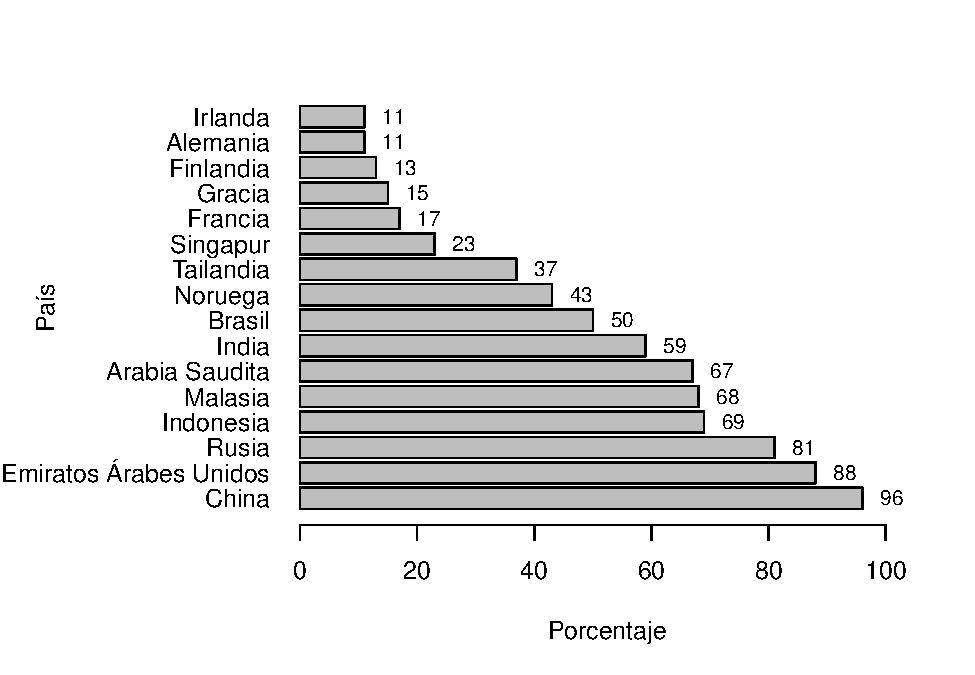
\includegraphics{Regulacion_files/figure-latex/fig1-1.pdf}
\caption{Participación pública en las 10 principales empresas por país,
años 2010-2011}
\end{figure}

Fuente: \citet{Kowalski2013}.

Por su parte \citet{Jones1982} consideran que el porcentaje de
participación de las empresas públicas en el PBI de los países en
desarrollo se mueve en un rango del 7\% al 15\%, independientemente de
la forma de organización que adopte la economía en cuestión. Las
situaciones que observan fuera de este rango se deben fundamentalmente a
una dotación de recursos diferentes, tal el caso de los países con
fuertes recursos en la minería donde la participación pública suele ser
alta, debido a las fuertes inversiones que se requieren en ese sector
que, en general, se considera estratégico.

En aquellos sectores de la economía donde la tecnología de producción de
bienes y servicios se caracteriza por la existencia de importantes
inversiones fijas y hundidas, \footnote{Las inversiones hundidas son
  aquellas que una vez realizadas no pueden asignarse a otros usos más
  allá de los previstos originalmente.} la provisión de estos servicios
públicos resulta más eficiente si la realiza un número limitado de
oferentes y, en algunos casos, sólo si lo hace una única empresa.
\footnote{A vía de ejemplo, la inversión prevista por ANTEL para
  instalar fibra óptica al hogar para la transmisión de datos alcanza a
  U\$S 550 millones, aproximadamente el 50\% de la facturación de la
  empresa en 2012.} La necesidad de contar con activos fijos que tienen
un costo muy importante y que en sí mismos permiten atender a toda la
demanda, lleva a que la duplicación de esta infraestructura sea
ineficiente desde el punto de vista económico. Entre estos sectores se
encuentran la transmisión de energía, agua potable, saneamiento,
transporte aéreo y terrestre, minería o transmisión de datos. En varios
países desarrollados y en desarrollo estas actividades las realizan
empresas públicas, como puede verse en el gráfico @ref(fig:fig2) que
presenta el porcentaje de empresas públicas por sector en las mayores
2.000 empresas.

\begin{figure}
\centering
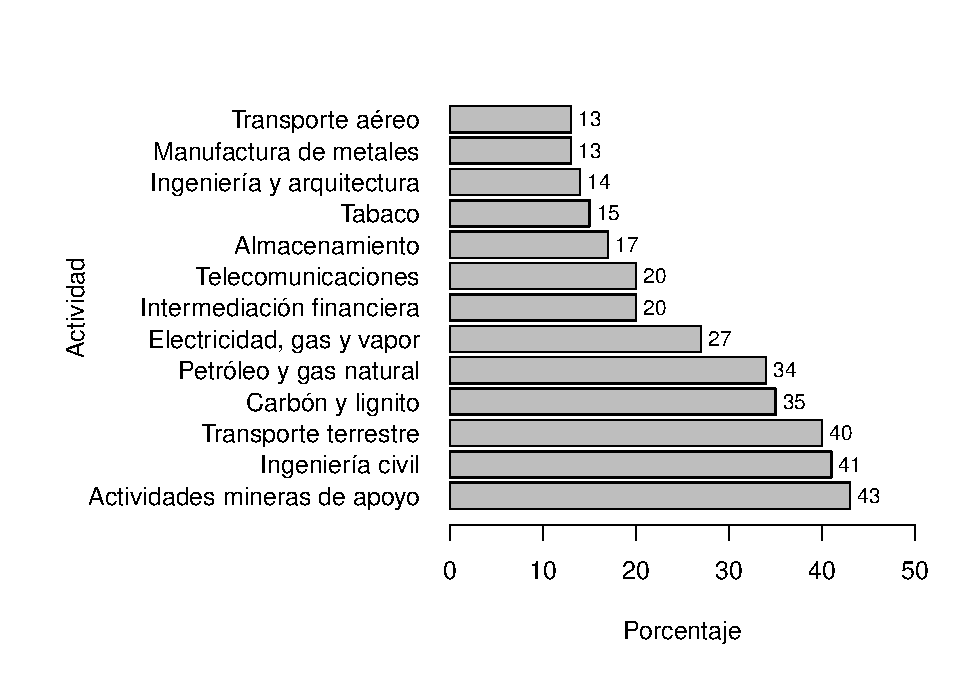
\includegraphics{Regulacion_files/figure-latex/fig2-1.pdf}
\caption{Participación pública por sector económico en las 2.000 mayores
empresas, años 2010-2011}
\end{figure}

Fuente: \citet{Kowalski2013}.

La discusión acerca de la propiedad de las empresas en estos sectores
donde opera un monopolio natural adquiere relevancia debido a que, en
general, los gobiernos no pueden suscribir contratos completos con las
firmas privadas. \citet{Laffont1993} al analizar las diferencias entre
una empresa pública y una privada regulada señalan que si los contratos
fueran completos entonces la propiedad de las empresas sería
irrelevante. En este caso el gobierno siempre podría diseñar un contrato
y hacerlo cumplir de forma de que la empresa privada lleve a cabo los
objetivos que se le impone; a su vez, la empresa privada podría realizar
esos objetivos sin temer expropiación alguna por parte del gobierno.

La imposibilidad de suscribir contratos completos responde a distintos
factores. Puede ser imposible prever todas las contingencias futuras o
resultar costoso redactarlas, por lo cual, cualquier contrato entre las
partes presentará lagunas o aspectos no resueltos. Aún si todas las
contingencias se incluyen en el contrato, puede ser imposible verificar
alguna de las variables relevantes. Por tanto, los contratos incompletos
impiden regular efectivamente a las empresas, en la medida en que alguna
de las variables relevantes no puede ser contratada \emph{ex ante}. En
estos casos, el derecho de propiedad residual sobre los activos permite
resolver los problemas contractuales (\citet{Hart1995};
\citet{Perotti2004}).

La literatura económica, por su parte, aborda extensamente la temática
de las empresas públicas, principalmente, en países de menor desarrollo
relativo. \footnote{Véase \citet{Jones1982}, \citet{WorldBank1995} y,
  para un análisis de las empresas en los países socialistas,
  \citet{Roland2000}.} Sin embargo la discusión de fondo sobre la
propiedad de las empresas es un tema que se encuentra lejos de estar
resuelto \citep{Hart2003}. Debe aclararse que la discusión relevante
sobre la propiedad de las empresas, para este trabajo, es sobre aquellas
que tienen características de monopolios naturales en todo o parte de
sus segmentos.

Esta discusión tuvo su momento de mayor desarrollo en los trabajos de
\citet{Lange1936}, \citet{Lange1937} y \citet{Lerner1944} sobre
socialismo de mercado (ver \citet{Coloma2004}). Los argumentos
económicos sobre los que se fundamenta la existencia de empresas
públicas se basan en diversas fallas de mercado, como el control del
poder de mercado de las empresas, el bajo desarrollo de los mercados de
capitales, así como la necesidad de distribuir el riesgo de esas
actividades entre el conjunto de la sociedad \citep{Sappington1987}.
Asimismo, se basan en el supuesto de que el gobierno actúa en forma
benevolente y que tiene como objetivo maximizar el bienestar de largo
plazo de la sociedad, entre otros (\citet{Dixit1997};
\citet{Martimort2006}).

Teorías más modernas consideran las complejidades que tienen los
gobiernos para llevar adelante las políticas. Desde la posibilidad de la
captura por parte de grupos de interés, hasta la visión de la política
como un proceso influido por distintos actores y grupos de interés, la
visión de un gobierno imparcial y benevolente se ha transformado para
introducir la idea de que las decisiones políticas tienen lógica propia
\citep{Dixit1997}. En este marco, los costos de implementar una
determinada política por parte del Estado pueden ser mayores a los
beneficios que se buscan con ella.

En el capítulo @ref(\#reg-ec) se analizó la teoría de Shleifer (2005)
que señala que la propiedad pública de empresas es una solución por
defecto en aquellos casos donde el gobierno no logra alinear el
comportamiento de las empresas con el interés de la sociedad mediante
otras políticas públicas. En este marco, los gobiernos tienen un
continuo de instrumentos a su disposición para llevar a cabo sus
actividades y balancean dos pérdidas sociales opuestas: la expropiación
por parte de privados (desorden) y la expropiación por parte del Estado
(dictadura).

Todas las estrategias de control social de los negocios son imperfectas,
y el diseño institucional concreto implica elegir entre alternativas
imperfectas. El ordenamiento privado aparece en un extremo, donde existe
un costo importante en términos de pérdidas asociadas a la expropiación
por parte de privados, pero baja por parte del Estado. El continuo pasa
por jueces independientes y organismos reguladores, hasta llegar a la
propiedad pública de las empresas en el otro extremo, donde los costos
de expropiación privada son bajos, pero altos los de expropiación por
parte del Estado.

\citet{Perotti2004} señala que coexisten dos tipos de problemas que
pueden desembocar en la necesidad de que la propiedad de las empresas
sea pública. Por un lado, el que denomina problema de compromiso público
e implica la imposibilidad de algunos gobiernos de no renegociar sus
políticas hacia el sector privado, lo que resulta en el desaliento de la
inversión privada. \citet{Bergara2003} desarrolla esta visión
enfatizando en el diseño institucional de las políticas públicas. Por
otro, los que denomina problemas de compromiso privado, que hacen
referencia a las dificultades del regulador para controlar en forma
efectiva las decisiones de empresas privadas. En cualquiera de los dos
escenarios,

la empresa pública aparece como un sustituto a la privada, debido a
problemas de compromiso de distinta naturaleza. Otras veces los
problemas están vinculados al monto de los recursos necesarios para el
desarrollo de estas actividades. Si los mercados de capitales están poco
desarrollados y la economía no resulta atractiva para los inversores
externos, entonces sólo los Estados pueden movilizar recursos para
llevar a cabo determinadas actividades económicas (\citet{Mintz1982};
\citet{LaPorta1998}).

En el caso de Uruguay, este fue uno de los principales problemas que
determinaron la conformación de las empresas públicas. \citet{Jones1982}
señalan otros factores, políticos y sociales, que determinan el
surgimiento de las empresas públicas, y los agrupan en cuatro:

\begin{enumerate}
\def\labelenumi{\arabic{enumi}.}
\item
  \textbf{Predilección ideológica}: es la creencia a priori de que
  ciertas formas de propiedad son preferibles. No necesariamente es una
  decisión irracional, a vía de ejemplo, señalan que con el fin de
  mejorar la distribución del ingreso, el medio utilizado por los países
  escandinavos ha sido los impuestos, mientras que en los países de
  Europa del Este ha sido la producción pública.
\item
  \textbf{Adquisición o consolidación de poder político o económico}: la
  propiedad y el control de unidades económicas son instrumentos para
  que los intereses de ciertos grupos avancen y otros se frustren.
\item
  \textbf{Herencia histórica}: independientemente de cuál haya sido el
  origen de las empresas públicas, una vez que se constituyen y
  permanecen durante un período significativo de tiempo, llevan a una
  fuerte inercia que hace facti- ble su permanencia más allá de aspectos
  ideológicos o de desempeño.
\item
  \textbf{Pragmatismo político}: la empresa pública es simplemente una
  herramienta, entre varias, que tiene el gobierno a su disposición para
  modificar el comportamiento de una economía mixta.
\end{enumerate}

Del punto de vista de las sociedades, alcanzar un determinado tipo de
arreglo institucional (privado-público) implica valoraciones diferentes
respecto al peso que se otorga a los distintos costos económicos
---eficiencia productiva y asignativa, accesos a financiamiento--- o
políticos ---electorales, desorden social, entre otros---. En general,
las empresas públicas operan en sectores de actividad que se
caracterizan por ser monopolios naturales donde, como se analizó
anteriormente, los productos son ampliamente consumidos; existen
importantes economías de escala o de ámbito; y, las inversiones, en gran
parte, son hundidas. Por lo que, en estos mercados, resulta imposible
desentrañar lo económico de lo político (\citet{Bergara2003};
\citet{Spiller2013})

\hypertarget{caracteruxedsticas-de-las-empresas-puxfablicas}{%
\section{Características de las Empresas
Públicas}\label{caracteruxedsticas-de-las-empresas-puxfablicas}}

Las empresas públicas son organizaciones híbridas \citep{Jones1982}. Por
un lado, tiene características similares a cualquier empresa privada
(vende un producto y realiza las funciones de producción, publicidad y
marketing de sus productos) y enfrenta las presiones del mercado. Por
otro, como organización pública controlada por el gobierno, enfrenta
presiones directas o indirectas de la burocracia, los políticos, y el
público en general. Sin embargo, esta mezcla de características hace que
las empresas públicas sean unidades diferentes a los gobiernos y a las
empresas privadas.

La principal característica del gobierno de las empresas públicas
implica que éstas se enfrenten a múltiples principales
(\citet{Dixit1998} y \citet{Dixit1997}; \citet{Martimort1996};
\citet{Tirole1994}). La teoría del principal-agente plantea que existe
una relación de agencia cuando una parte (el principal) delega en otra
la realización de una tarea (el agente). Las acciones del agente tienen
impacto sobre el bienestar del principal y existe, además, asimetría de
información entre las partes respecto a alguna de las variables
relevantes que determinan el desempeño del agente. Cuando varios
principales delegan en un mismo agente la realización de una tarea, cada
principal procurará que éste realice la tarea según sus propios
intereses u objetivos por sobre los de los demás.

Como consecuencia, las empresas deben perseguir múltiples objetivos,
algunos de los cuales pueden llegar a ser antagónicos entre sí
\citep{Tirole1994}. Estos abarcan tanto objetivos comerciales como no
comerciales: beneficios, redistribución de ingresos, subsidios a
regiones o sectores específicos, generación de empleo, obtención de
divisas, aumentar la probabilidad de reelección del partido en el poder,
entre otros. Esta multiplicidad de objetivos tiene impactos sobre la
eficiencia productiva de las empresas públicas.

\citet{Miltnisky2001} señala que las empresas públicas juegan, en
términos institucionales, dos juegos que tienen reglas distintas: el
político y el económico. \footnote{\citet{Dixit1997} señala que estas
  organizaciones operan directamente en un marco político.} En este
marco, las instituciones establecen lo que los agentes pueden o no
hacer, para fomentar la cooperación entre ellos. Señala la imposibilidad
de jugar los dos juegos a la vez, dado que los objetivos de un juego se
contradicen con los del otro. El juego económico es evaluar la
eficiencia en la provisión de los productos, mientras que el juego
político busca captar o fidelizar votantes. El juego económico requiere
normas flexibles de contratación y compra, el juego político impone
normas rígidas similares a las del propio Estado. El juego económico
requiere autonomía para el cumplimiento de los objetivos, el juego
político establece restricciones a la forma de llevar a cabo el negocio.
El juego económico requiere gerentes y funcionarios elegidos por sus
capacidades, el juego político los elige según sus voluntades.

\citet{Martimort1996} destaca otra dimensión asociado a la naturaleza de
múltiples principales en que se encuentran las empresas públicas. En
este marco, las asimetrías de información provocan un efecto de free
rider entre reguladores que reduce el control que cada uno ejerce sobre
la empresa. Aun cuando las tareas de los reguladores sean sustitutas
entre sí, el nivel de control que estos ejercen es menor al que
ejercería un único principal.

\citet{Miltnisky2001} y \citet{Jones1982} enfatizan la idea de que es
complejo medir los resultados de las empresas públicas debido a sus
múltiples objetivos o reglas de juego. Alcanzar un objetivo
-universalizar un servicio, como llevar energía eléctrica a todas las
escuelas- puede ir en detrimento de otro -maximización de beneficios-.
En otros términos, en la ecuación objetivo de quienes conducen empresas
privadas entra el beneficio, mientras que en las empresas públicas el
beneficio tiene un peso mucho menor dado que el principal objetivo pasa
a ser obtener apoyo político para la gestión. En última instancia, los
directores de empresas públicas son actores políticos que se mueven
según sus propias reglas de juego.

Por último, los incentivos en las empresas públicas son más débiles que
en las privadas \citep{Dixit1997}. La naturaleza multidimensional de las
tareas que realizan estas empresas implica que incentivar un objetivo
puede llevar a que otro de los objetivos no sea alcanzado. Por ello, los
principales no pueden establecer mecanismos para incentivar al agente:
el incentivo de uno será un desincentivo para otro. Si un ministerio
quiere establecer premios a la eficiencia, pero otro busca premiar la
cobertura del servicio, entonces los incentivos se cancelan entre sí y
no hay cambios en el comportamiento del agente. En el caso extremo, si
el número de principales es importante, se puede llegar a la inacción de
la empresa.

\hypertarget{empresa-puxfablica-y-su-eficiencia}{%
\section{Empresa pública y su
eficiencia}\label{empresa-puxfablica-y-su-eficiencia}}

A las empresas públicas, en la mayoría de los países, se las considera
ineficientes desde el punto de vista productivo. Según
\citet{Jones1982}, esto no es sorprendente debido a su doble
característica de empresa y de organización pública que sufre presiones
diversas, por un lado las del mercado y por el otro las del poder
político. En esta dualidad de objetivos el resultado de la firma suele
ser sub-óptimo para los estándares del mercado y/o del poder político.
En consecuencia, la existencia de múltiples principales es, en sí mismo,
una fuente importante de ineficiencia para las empresas públicas.

Perseguir objetivos diversos y muchas veces contradictorios, la mayor
laxitud en los controles por parte de principales que hacen free riding
entre ellos y la dificultad para establecer incentivos fuertes al
desempeño se asocian para impedir que el resultado de las empresas
públicas sea igual de eficiente al de las privadas.

La imposición de fines políticos a las empresas públicas
\citep{Shleifer1994} tiene su contrapartida en controles diferenciados
respecto a las privadas. En efecto, como la empresa pública está sujeta
a controles políticos, los procesos de contratación de funcionarios, de
compra e inversiones tienden a ser más rígidos que en una empresa
privada. Además, las autorizaciones que requieren a los efectos de las
inversiones, no necesariamente tienen que ver con la eficiencia sino que
pueden atender a otros fines, como evitar que crezca el endeudamiento
del país.

El control político de las empresas facilita su utilización como un
instrumento más de la política, ya sea partidaria o de gobierno
\citep{Miltnisky2001}, por lo que se requieren salvaguardas para impedir
que las empresas sean vaciadas y quiebren en los casos en que no existan
restricciones legales al respecto. A estos problemas se agregan los
controles que enfrentan estas empresas por su naturaleza política. Las
empresas públicas no pueden tener, por definición, las mayores
libertades y flexibilidades de las privadas para contratar, licitar y
comprar. Asimismo, muchas veces asumen en sus costos -en el marco de sus
objetivos políticos implícitos- acciones que no realizan las empresas
privadas, por las cuales no obtienen compensación del principal.

Por otra parte, la literatura abunda sobre la ineficiencia productiva de
las empresas públicas y, como lo señalan \citet{Jones1982}, entre las
principales causas de este comportamiento se encuentra que, en general,
estas empresas:

\begin{itemize}
\item
  operan bajo sistemas burocráticos que controlan procesos antes que
  resultados, a través de procedimientos que demandan múltiples
  aprobaciones ministeriales y que generan demoras que pueden resultar
  muy costosas cuando las empresas operan en mercados dinámicos;
\item
  son utilizadas para transferir ingresos del sector público a
  diferentes grupos de interés, mediante mecanismos poco transparentes
  frente a quienes pagan el costo en términos de mayores impuestos,
  inflación y menores gastos gubernamentales en salud, educación y
  bienestar; y
\item
  el desempeño gerencial no puede evaluarse ya que resulta imposible
  distinguir un desempeño bueno de uno malo, puesto que cualquier efecto
  de las decisiones de los gerentes sobre los beneficios de la empresa
  pueden esconderse, imputando el mismo a políticas gubernamentales
  sobre precios que afectan sus productos y sus insumos. Así los
  gerentes tienen pocos incentivos a controlar los costos, porque pueden
  esconder las ineficiencias y, además, porque, en general, la
  estructura salarial pública no permite otorgar bonificaciones por los
  resultados obtenidos.
\end{itemize}

En conjunto, estos elementos ayudan a explicar por qué es más probable
que las empresas públicas enfrenten un escenario de menor eficiencia
productiva que las empresas privadas. \^{}{[}Este resultado ha sido
recogido en el informe del año 1995 del Banco Mundial
\citep{WorldBank1995}. El problema de ineficiencia de las empresas
públicas es un tema ampliamente discutido en la literatura, en
particular aquella que estudia la caída del sistema socialista
\citep{Roland2000}. Esta literatura agrega una dimensión de compromiso
dinámico adicional que enfrentan los gobiernos que tienen empresas a su
cargo.

En general, la evidencia ha demostrado que muchas veces las empresas
públicas actúan bajo un marco de restricciones presupuestales blandas.
Este efecto, identificado inicialmente por \citet{Kornai1980} refiere a
que los gobiernos no pueden comprometerse en forma creíble a no
refinanciar a estas empresas cuando presentan pérdidas. Ello relaja ex
ante los incentivos de las empresas a ser eficientes. El problema es de
compromiso dinámico. El gobierno quiere comprometerse a no relajar la
restricción de la empresa, pero como tiene activos hundidos en ellas, a
la hora de ejecutar su amenaza la misma no es creíble. \footnote{La
  referencia clásica es \citet{Dewatripont1995}. Véase también
  \citet{Bergara2011} para un análisis de cómo el gobierno puede imponer
  una restricción presupuestal blanda a las empresas.} Sabiendo eso, la
empresa tiene menores incentivos a esforzarse al inicio dado que,
cualquiera sea el resultado, será refinanciada.

Debe señalarse que el problema de las restricciones presupuestales
blandas no es un problema excluyente de las empresas públicas. En
Uruguay muchas empresas privadas se han movido bajo esa lógica
\citep{Vaz1993}. Sin embargo, en las empresas públicas uruguayas, hay un
consenso implícito de que estas no quiebran. {[}La Administración de
Ferrocarriles del Estado (AFE) en Uruguay, recibe subsidios desde hace
años y no ha cerrado aún.{]} Ello determina que tarde o temprano los
precios van a acomodar las cuentas de las empresas, o en algún momento
algún director impulsará la gestión de la misma. En otros términos, las
empresas responden en forma menos intensa a los incentivos de precio y,
por tanto, este no sirve como el único instrumento regulatorio.

Un último elemento que señalan \citet{Sappington1987} refiere a que la
propiedad pública de las empresas reduce los costos de transacción de
renegociar los objetivos, frente a hacerlo con empresas privadas. Por
ello, el gobierno no puede comprometerse a no renegociar sus objetivos
cuando la empresa es pública, a menos que las privatice.

La discusión anterior presenta una división entre las posibles fuentes
de eficiencia relativa de las empresas públicas. Por un lado, la
propiedad de las mismas puede no generar los incentivos suficientes para
una adecuada gestión, debido a los diversos objetivos y múltiples
principales. Por otra parte, el entorno en el que operan las empresas
públicas, donde muchas veces la competencia es limitada o existen
restricciones presupuestales blandas no les permite ser eficientes.

\citet{Bartel2005} analizan estas fuentes de posibles ineficiencias y
encuentran que ambas tienen un rol en la explicación de la eficiencia
relativa de las empresas. Encuentran que las empresas públicas son menos
eficientes que las privadas, dado un mismo entorno competitivo y
financiamiento del gobierno. Sin embargo, el entorno en el que operan es
relevante dado que sólo las empresas que reciben financiamiento del
gobierno o están aisladas de la competencia tienen un peor desempeño que
las empresas privadas.

En este sentido, sostienen que la privatización de las empresas y la
reforma del entorno en el que operan son políticas sustitutas. Es decir,
un incremento de la competencia o la reducción de subsidios permitirían
alcanzar resultados similares a la privatización en términos de mejora
de eficiencia. Este elemento, que muchas veces se soslaya, pone el
énfasis en la necesidad de que las empresas públicas se muevan en un
entorno competitivo y sin subsidios, siempre que ello sea posible.

En el cuadro @ref(tab:cuadro5) se resumen las principales diferencias
entre empresas públicas y privadas, consideradas anteriormente.

\begin{longtable}[]{@{}lll@{}}
\caption{Diferencias entre empresas públicas y privadas}\tabularnewline
\toprule
Dimensión & Empresa privada & Empresa pública\tabularnewline
\midrule
\endfirsthead
\toprule
Dimensión & Empresa privada & Empresa pública\tabularnewline
\midrule
\endhead
Principal & Único & Múltiplos\tabularnewline
Objetivos & Maximización de beneficios & Múltiples, a veces
difusos\tabularnewline
Potencia de incentivos & Fuerte & Baja\tabularnewline
Restricción presupuestal & Dura & Blanda\tabularnewline
Ajuste ante imprevistos & Renegociación costosa &
Flexible\tabularnewline
\bottomrule
\end{longtable}

Fuente: elaboración propia.

Por su parte, en la sección siguiente se desarrollará la idea de lograr
un entorno competitivo en el que las empresas públicas operen, en el
marco de los instrumentos regulatorios para dichas empresas.

\hypertarget{la-regulaciuxf3n-de-empresas-puxfablicas}{%
\section{La regulación de empresas
públicas}\label{la-regulaciuxf3n-de-empresas-puxfablicas}}

\hypertarget{regulaciuxf3n-de-actividades-en-ruxe9gimen-monopolio}{%
\subsection{Regulación de actividades en régimen
monopolio}\label{regulaciuxf3n-de-actividades-en-ruxe9gimen-monopolio}}

Para aquellos que ven a la producción de bienes y servicios por parte
del Estado como una forma alternativa de resguardar el poder de mercado
de las empresas, la propiedad pública de las empresas es una alternativa
a la regulación (\citet{Shleifer2005}; \citet{Viscusi2005}). En
consecuencia, en esta situación la regulación de las empresas públicas
no tendría sentido ya que el principal problema que se considera en el
monopolio privado -el poder de mercado- queda resuelto a través de la
propiedad estatal.

Sin embargo, cuando operan empresas de propiedad estatal surgen
problemas distintos al poder de mercado. En este caso, el principal
problema a considerar, como lo muestra la evidencia empírica de los
países del bloque socialista, es que las empresas públicas operan,
muchas veces, en forma ineficiente y sus directores no son penalizados
por ello.

Si bien la eficiencia es un problema al que también se enfrentan las
empresas monopólicas privadas, en la medida en que no hay presión
competitiva en esos mercados, esto resulta de segundo orden en relación
con el problema principal del monopolio, el poder de mercado. En el caso
de la empresa pública el orden de los problemas se invierte: la
eficiencia productiva pasa a ser el problema fundamental mientras que el
poder de mercado pasa a un segundo plano (\citet{Roland2000},
\citet{WorldBank1995}).

Por tanto, la regulación y la propiedad pública de las empresas no son
conceptos sustitutos, sino que resultan complementarios. La regulación,
cuando refiere a empresas públicas, persigue objetivos distintos a la
regulación de empresas privadas. La regulación de empresas públicas
debería tener como principal objetivo alcanzar la eficiencia económica,
en particular la eficiencia productiva. La regulación debe inducir a las
empresas públicas a ser costo eficiente, sustituyendo al mercado para
generar esos incentivos. Ello sin descuidar la sustentabilidad de largo
plazo que permita mantener los servicios en el futuro.

La naturaleza económica y política de las empresas públicas hace que su
regulación sea más compleja que la de las empresas privadas. Para estas
empresas la maximización de beneficio es uno de los múltiples objetivos
que guían su accionar. Asimismo, dentro de cierto margen, operan bajo un
régimen implícito de restricciones presupuestales blandas. Ambas
características atentan contra la minimización de los costos.

\citet{Laffont1993} diferencian dos tipos de controles que puede
establecer el gobierno. Por un lado, el control externo, que consideran
las variables que vinculan a la empresa con los agentes externos a ella:
consumidores (regulación de precios, calidad); competidores (regulación
de entrada, tarifa de acceso); contribuyentes (auditoría de costo). Por
otro, el control interno que implica el control de los insumos y del
proceso de minimización de costos, a través de esquemas de incentivos, o
la intervención sobre decisiones que involucran el empleo, la
localización, el tipo de inversión o el endeudamiento.

En la regulación de estas empresas, el instrumento clave utilizado para
incidir en el comportamiento de las empresas privadas, la fijación de la
tarifa, pierde fuerza ya que por sí sola no puede resolver los problemas
de eficiencia de las empresas públicas. Como estas empresas están
sometidas a un régimen implícito de restricciones blandas, entonces la
fijación de tarifas como instrumento regulatorio no es suficiente para
transmitir los incentivos necesarios para la adopción de la tecnología
eficiente. Si el regulador conoce el costo de la tecnología eficiente, y
la eficiencia fuera el único objetivo, podría fijar el precio de forma
de que sea igual a este costo.

Sin embargo, si este precio implica pérdidas para la empresa, y esta
sabe que no quebrará, entonces este instrumento no genera los incentivos
para la adopción de una mejor tecnología. En la terminología de
\citet{Laffont1993} se requiere influir sobre las variables de control
externo, pero también sobre las de control interno para alcanzar la
eficiencia. Por tanto, la regulación debe combinar la regulación de
precio con la regulación del gobierno corporativo, incentivando las
buenas prácticas empresariales \citep{Berg2013}.

La regulación de precio debe complementarse con otras medidas de gestión
(gobierno corporativo) que atiendan a la naturaleza híbrida de las
empresas. \citet{Andres2011} presentan una revisión del estado del
gobierno corporativo de las empresas públicas en América Latina, y
encuentran una gran dispersión en la incorporación de mejores prácticas,
con una mayor incorporación de las mismas en las empresas de energía
eléctrica con relación a las de agua.

Las buenas prácticas de gobierno corporativo de la OECD incluyen una
serie de criterios generales para el manejo de las empresas públicas.
Transparencia y divulgación; explicitación clara de los objetivos;
separación de los roles productivos y reguladores; responsabilidad,
competencia y objetividad de los directores de las empresas, son
conceptos que apuntan a una adecuada y eficiente gestión de las
empresas, independientemente de sus objetivos \citep{OECD2011}.

En este marco, el regulador, como parte del Estado pero también como
órgano técnico independiente, tiene que participar en la determinación
técnica de las tarifas de las empresas públicas, aun cuando este
instrumento tenga un menor efecto como incentivo para inducir el
comportamiento de estas empresas que en el caso de las empresas
privadas, ya que se requiere un control técnico que sirva como contralor
y balance de la ineficiencia relativa de las primeras.

El problema real que enfrenta la regulación de empresas públicas, es
definir el papel legítimo de los diferentes órganos estatales y las
dimensiones del control social que se requiere en el funcionamiento de
estas empresas. En la literatura de la administración pública, el
problema es el balance entre la autonomía suficiente para desarrollar
las actividades del negocio sin las dificultades que implican las
rigideces inherentes a las estructuras burocráticas del gobierno, y la
rendición de cuentas al gobierno y al Parlamento, organismos que dictan
los objetivos de estas empresas.

\citet{Ramamurti1991} establece que la autonomía gerencial es el método
que asegura que estas empresas realicen en forma eficiente sus
actividades, siempre y cuando se combinen con una rendición de cuentas
transparente y a tiempo. Este autor señala que el control de la
actividad de las empresas tiene dos enfoques posibles. En primer lugar,
el control puede ser cualitativo y enfocarse sobre los resultados de la
empresa. En este caso, la atención se centra en establecer los objetivos
y otorgar autonomía a la empresa para elegir la tecnología para
alcanzarlos.

En segundo término, el enfoque puede estar en el control cuantitativo de
los procesos de producción o, de otra forma, estudiando la forma en la
que los insumos se convierten en productos. Ello se traduce en controles
constantes de forma de verificar el proceso de producción.

En el primer caso, existe una importante autonomía de gestión u
operativa, mientras que en el segundo existe una gran autonomía para
fijar los objetivos estratégicos de la empresa. En términos generales,
los gerentes deberían tener baja autonomía en la definición de la
estrategia y alta autonomía en materia operacional, mientras que los
gobiernos deberían ser activos en la fijación de objetivos, estrategias
y políticas, otorgando a los gerentes amplia libertad en la
implementación de los programas aprobados.

Sin embargo, en el marco del gobierno corporativo, los gerentes de las
empresas públicas tratan de influenciar el proceso de especificación de
metas y resistir la imposición de ciertos objetivos, al tiempo que
reclaman el derecho de participar en su formulación. Asimismo, según
\citet{Jones1991} muchos gobiernos no están organizados para realizar un
control por resultado eficiente y, en consecuencia, tratan de controlar
una variedad de procesos internos, resultando en excesivo control de
baja calidad.

Por su parte, \citet{Aharoni1982} sostiene que en muchos países las
estructuras de control no están bien definidas y el ejecutivo (consejo,
directorio) no puede disciplinar o reemplazar al gerente, al menos sin
una larga negociación con el ministro y otros agentes gubernamentales.
Asimismo, considera que la experiencia muestra que en las firmas más
grandes, más independientes del gobierno (genera sus propios recursos) y
que utilizan información más técnica para su operación, mayor es el
poder que se concentra en la gerencia y, por lo tanto, los gerentes
tienen más grados de libertad para fijar las metas a alcanzar por la
empresa. En estos casos, el regulador es el único que puede ejercer el
balance en el control de las decisiones técnicas de las empresas
públicas.

En otros términos, el regulador es el órgano técnico que puede asesorar
a la toma de decisiones cuando existe asimetría de información entre los
gerentes de las empresas y el sector político que define los
lineamientos. En este marco, en Uruguay es claro que hay que repensar el
rol que cumplen los órganos reguladores sectoriales. Hay que incorporar
nuevas funciones a su menú de instrumentos y balancear sus roles de
regulador y asesor en la fijación de las distintas variables, tanto
internas como externas a la empresa.

\citet{Ramamurti1991}, por su parte, señala una serie de barreras que
enfrentan los gobiernos a la hora de incrementar la calidad de los
controles sobre las empresas públicas. Estas incluyen:

\begin{enumerate}
\def\labelenumi{\arabic{enumi}.}
\tightlist
\item
  barreras técnicas: definir el criterio más adecuado para medir la
  actuación de las empresas, discernir los resultados asociados a las
  decisiones gerenciales, balancear las metas de corto y largo plazo a
  través de planificación estratégica; y
\item
  barreras organizacionales: asimetría en la experiencia e información,
  conflicto entre los múltiples objetivos, dificultades de coordinación
  en el ámbito de una organización imprecisa como el Estado.
\end{enumerate}

Sólo organismos reguladores independientes y eficientes pueden levantar
las barreras mencionadas y colaborar en la valoración de los objetivos
no económicos, bajo el entendido que cualquier objetivo de estas
empresas se desarrolla a través de instrumentos económicos y, por tanto,
son siempre cuantificables ex post.

\citet{Berg2013}, por su parte, señala que la tendencia reciente en
materia regulatoria lleva a establecer agencias reguladoras
relativamente independientes con el objetivo de reducir el poder de los
ministerios gubernamentales responsables de la política sectorial sobre
el funcionamiento de las empresas públicas. Por otra parte, la creación
de las agencias reguladoras, en última instancia, implica poner un
principal más a la empresa pública, que ya tiene diversos principales
que fijan sus objetivos. Estas agencias deben jugar un papel en
supervisar al sector en que operan las empresas públicas, promover la
transparencia, y establecer incentivos para mejorar los resultados, y no
debería fijar objetivos nuevos para la misma.

A su vez, la existencia de múltiples objetivos en las empresas públicas,
introduce un problema adicional para la regulación. Esta realidad
determina que es poco factible contratar objetivos con las empresas,
dado que el sistema político tiene incentivos a revisar y renegociar
estos objetivos. Por un lado, algunos objetivos pueden entrar en
conflicto entre sí. Pero por otro, si los objetivos de los múltiples
principales cambian en forma muy volátil, no es posible determinar si es
la dirección de la empresa o los cambios los que provocan el resultado
observado. Esta diversidad y cambio reducen los incentivos que los
propios contratos de desempeño pretenden incentivar. Por tanto, no se
puede evaluar contractualmente el desempeño de los directores o gerentes
(\citet{Martimort1996}; \citet{Dixit1997}).

La regulación de las empresas públicas debe, por tanto, incluir diversas
dimensiones. En primer lugar, el regulador debe fijar el precio del
servicio, no dejarlo librado a la empresa dado que ello agudiza los
problemas de ineficiencia productiva. En este marco, un criterio creíble
sería un mecanismo de determinación de precios techo o incrementos
máximos para la empresa, determinados para un horizonte de mediano
plazo. Ello da previsibilidad a la empresa para planificar su proceso
productivo, por un lado, y, por otro, otorga credibilidad al regulador
al no someter la política regulatoria a renegociación constante.

En segundo lugar, las empresas públicas deben adoptar una serie de
principios que atiendan a las mejores prácticas de gobierno corporativo
(transparencia, auditoría, etc.). Estas deben incluir, también, la
separación contable de las actividades y transparentar los subsidios
cruzados entre ellas, así como el análisis costo beneficio de los
objetivos perseguidos independientemente de su naturaleza.

En tercer lugar, se debe transitar a un esquema donde los principales
establecen los objetivos o resultados esperados por la empresa de la
forma más objetiva y cuantificable posible. La empresa es la que debe
llevar esos objetivos a la práctica decidiendo el proceso productivo más
eficiente en el marco de la autonomía técnica que posee.

En cuarto lugar, existe un rol para que los reguladores asesoren a los
organismos involucrados en el control de gestión de la empresa, en
particular a aquel que tiene injerencia sobre el presupuesto y las
inversiones. Por otra parte, las empresas públicas están sometidas a
fuertes controles presupuestales y de inversión. Es sobre estos
controles que el órgano regulador puede aportar la visión técnica del
mercado.

En última instancia, el regulador es el órgano con las capacidades
técnicas para evaluar la coherencia del conjunto de objetivos, procesos
y tarifas propuestos, así como el presupuesto definido para alcanzarlos.
Algunos de estos cometidos pueden encontrarse dispersos entre distintos
organismos, mientras que otros no son controlados.

\hypertarget{regulaciuxf3n-de-actividades-en-competencia}{%
\subsection{Regulación de actividades en
competencia}\label{regulaciuxf3n-de-actividades-en-competencia}}

El problema regulatorio es diferente cuando las empresas públicas
compiten con otras empresas privadas en un sector de actividad. Aquí el
principio general debería ser el de no discriminación e iguales reglas
de juego para todos los actores, en particular la competencia entre
todos los agentes. En estos mercados la competencia puede adoptar las
dos dimensiones: competencia en el mercado, o competencia por el
mercado. Aislar a las empresas públicas de la competencia, al igual que
a las empresas privadas, sólo lleva al agravamiento de la ineficiencia
productiva.

Hay un elemento común que caracteriza a estos mercados: las empresas
públicas tienen algún monopolio en algún eslabón de la cadena de valor
del sector. Por ejemplo, la generación de energía eléctrica es un
mercado en competencia, pero la transmisión opera en un segmento
monopólico; la telefonía fija opera en un mercado monopólico, mientras
la telefonía móvil es un mercado competitivo; el refinamiento e
importación de combustibles se realiza en régimen de monopolio, mientras
que la distribución opera en competencia.

El regulador debe necesariamente intervenir en la interfase entre los
segmentos monopólicos y competitivos de forma de evitar que las empresas
públicas puedan tomar acciones que las beneficien a sí mismas, o incidan
limitando la competencia en los segmentos competitivos. No se requiere
que la empresa pública tenga intereses directos sobre ese segmento para
que se produzcan distorsiones. A vía de ejemplo, en Uruguay la empresa
pública de combustibles (ANCAP) tiene contratos con las estaciones que
dispensan gasolina, los que tienen impactos sobre la competencia en ese
mercado.

En resumen, el objetivo de la regulación en los mercados donde la
competencia es posible y operan empresas públicas debe ser fomentar la
competencia y fijar reglas iguales para todos los actores. Para ello,
debe instrumentarse la separación contable de las actividades de estas
empresas y hacer explícitos los subsidios cruzados entre sus
actividades, si alguna de ellas fuera monopólica.

\hypertarget{conclusiones-2}{%
\section{Conclusiones}\label{conclusiones-2}}

El análisis realizado permite comprender el funcionamiento y las
características de las empresas públicas y su vinculación con los
gobiernos o sea sus propietarios.

Si existe la posibilidad de suscribir contratos completos entre el
gobierno y las empresas que llevan adelante la producción, entonces la
propiedad de las empresas resulta irrelevante. En la medida en que
existen costos de transacción, los contratos entre las partes serán
incompletos y la propiedad pasa a ser relevante. En estos casos, la
propiedad pública de empresas es una solución por defecto, en los casos
donde el gobierno no logra alinear el comportamiento de las empresas con
el interés de la sociedad mediante otras políticas públicas.

Empresas públicas y privadas difieren en dos aspectos. En primer lugar,
las primeras responden a múltiples principales. Ello se traduce en un
conjunto de objetivos económicos, sociales y políticos, mientras que las
privadas sólo se guían por objetivos económicos. Ello determina que las
empresas públicas jueguen, en términos institucionales, dos juegos con
reglas distintas: el político y el económico. En segundo término, las
empresas públicas operan bajo un régimen implícito de restricciones
blandas. Si a esto se suma que tienden a actuar en mercados monopólicos,
entonces el resultado es potencialmente peligroso para la eficiencia de
estas empresas.

En este marco, la regulación es un instrumento complementario de la
propiedad pública. A diferencia de las empresas privadas que requieren
ser reguladas para evitar el abuso de posición dominante, las empresas
públicas requieren de la regulación para inducir un comportamiento
eficiente. Los múltiples objetivos y las restricciones blandas llevan a
que la eficiencia pueda ser un objetivo inferior con relación a otros
fines de la empresa. Por otra parte, los distintos ministerios
sectoriales que tienen injerencia sobre estas empresas no tienen como
objetivo de política lograr la eficiencia de las mismas, y si este fuera
uno de sus objetivos no podrían controlarlo debido a que se mueven con
asimetría de información respecto de las mismas.

El problema que enfrenta la regulación de empresas públicas es definir
el papel legítimo de los diferentes órganos estatales y las dimensiones
del control social que se requiere en el funcionamiento de estas
empresas. En términos de administración pública, alcanzar el balance
adecuado entre autonomía suficiente para desarrollar las actividades del
negocio sin las dificultades que generan las estructuras burocráticas
del gobierno, y la rendición de cuentas transparente y en tiempo a los
organismos que dictan los objetivos de estas empresas (gobierno y
Parlamento).

La existencia de organismos reguladores independientes y eficientes
permite levantar las barreras técnicas y organizacionales que enfrentan
los gobiernos a la hora de incrementar la calidad de los controles sobre
las empresas públicas.

La regulación de empresas públicas debería comprender las siguientes
dimensiones: el regulador debería fijar el precio techo o incrementos
máximos para la empresa para un horizonte de mediano plazo; las empresas
deberían adoptar principios que atiendan a las mejores prácticas de
gobierno corporativo; los principales deberían establecer los objetivos
o resultados esperados de forma objetiva y cuantificable; los
reguladores deberían asesorar a los organismos involucrados en el
control de gestión de la empresa (presupuesto e inversiones).

Cuando las empresas públicas participan en mercados en competencia, el
regulador debe intervenir en la interfase entre los segmentos
monopólicos y competitivos de forma de evitar que las empresas públicas
realicen acciones que las beneficien o limiten la competencia en los
segmentos competitivos. En definitiva, el regulador debe fomentar la
competencia y fijar reglas iguales para todos los actores.

\hypertarget{eepp-uy}{%
\chapter[Empresas públicas: el caso uruguayo ]{\texorpdfstring{Empresas
públicas: el caso uruguayo \footnote{Basado en el marco del acuerdo de
  cooperación entre la Facultad de Ciencias Sociales de la UdelaR y la
  Unidad Reguladora de los Servicios de Energía y Agua (URSEA) y contó
  con financiamiento de la Corporación Andina de Fomento (CAF).}}{Empresas públicas: el caso uruguayo }}\label{eepp-uy}}

Rosario Domingo Leandro Zipitría

Como se discutió en el capítulo @ref(reg-eepp), la existencia de
empresas públicas es un fenómeno habitual y económicamente
significativo, pudiendo encontrarse empresas públicas en diversos
sectores relevantes de la actividad económica en la mayoría de los
países. En el caso de la economía uruguaya, en particular, las empresas
públicas también son actores relevantes. Los servicios que prestan estas
empresas alcanzan al 12\% de la canasta del Índice de Precios al Consumo
(IPC), \footnote{Se consideraron los rubros agua, saneamiento,
  electricidad, gas por red, supergas, nafta, gas oil, telefonía fija y
  celular.} los gastos en que incurren representan un 10\% del Producto
Bruto Interno (PBI), \footnote{\citet{WorldBank2014}} y algunas de ellas
representan una fuente de ingresos para el gobierno central. \footnote{\citet{WorldBank1995}
  e información del MEF tomada del siguiente
  \href{http://www.mef.gub.uy/indicadores.php}{sitio}.}

La literatura económica, por su parte, aborda extensamente la temática
de las empresas públicas, principalmente, en países en vías de
desarrollo. \footnote{En el capítulo @ref(\#reg-eepp) se desarrolla esta
  temática. Una bibliografía de referencia es \citet{Jones1982},
  \citet{WorldBank1995}, y para un análisis de las empresas en los
  países socialistas, \citet{Roland2000}.} En este marco, este trabajo
analiza la existencia de empresas públicas en América Latina, el proceso
de creación y la situación actual de las empresas públicas en Uruguay,
así como de las unidades reguladoras correspondientes. La primera
sección presenta brevemente la evolución de las empresas públicas en la
región. La segunda presenta la génesis y creación de las empresas
públicas en Uruguay. En la tercera se analiza la situación de los
principales mercados en que operan las empresas públicas uruguayas,
mientras que en la cuarta y en la quinta se consideran los mecanismos de
regulación establecidos para estas empresas en América Latina y en
Uruguay, respectivamente. Finalmente, se caracterizar el marco jurídico
institucional en el que operan empresas y reguladores en Uruguay.

\hypertarget{empresas-puxfablicas-en-amuxe9rica-latina}{%
\section{Empresas Públicas en América
Latina}\label{empresas-puxfablicas-en-amuxe9rica-latina}}

Desde fines del siglo XIX se pueden encontrar en muchos países
latinoamericanos, empresas de propiedad estatal actuando en sectores
claves de la economía. A fines de ese siglo y comienzos del siglo XX,
estos países se encontraban en una fase primaria de su desarrollo
económico. Los problemas técnicos que enfrentaba el Estado para poder
regular los sectores de infraestructura de transporte y comunicación,
necesarios para el desarrollo de la actividad exportadora, y las fallas
en los mercados de capitales fomentó el surgimiento de empresas
estatales en estos mercados. En general, la presencia del Estado en
estas actividades respondía a la sensibilidad política de las mismas
(suministro de agua potable, transporte, etc.) al hacerse cargo de
servicios que dejaban de atender las empresas extranjeras.

A partir de los años treinta del siglo pasado y como consecuencia de la
crisis mundial que generó dificultades para adquirir productos
manufacturados, los países de la región se plantean el desarrollo de una
industria liviana orientada al mercado interno. Este proceso fue
promovido por nuevos actores políticos, económicos y sociales que
demandaban un papel más activo del Estado en las áreas que se consideran
estratégicas para el crecimiento económico. En las décadas del 30 y del
40 puede observarse una creciente participación del Estado en los
sectores de energía e infraestructura.

En este período se producen, también, una serie de nacionalizaciones de
empresas extranjeras que operaban en algunos servicios públicos y en
sectores extractivos, donde se concentraban las riquezas básicas de
muchas de estas economías. Estas nacionalizaciones se debieron tanto a
motivos políticos, como al cese de las concesiones otorgadas a las
empresas extranjeras y a la necesidad de rescatar aquellas empresas que
presentaban muy baja rentabilidad.

A mediados del siglo XX, como consecuencia del agotamiento del modelo
exportador primario y de las propuestas de desarrollo surgidas desde la
CEPAL, la mayoría de los países de la región iniciaron un proceso de
sustitución de importaciones que implicó desarrollar una industria
pesada, para lo cual fue necesario el apoyo de los estados nacionales.
Este apoyo no sólo incluyó el diseño de diversas políticas económicas
-inversión pública, cambiaria, arancelaria, fiscal, etc.- sino que
también implicó que el Estado actuara como empresario, con el objetivo
de suministrar bienes y servicios necesarios para el proceso de
industrialización.

En el período 1950-1970, las empresas de propiedad estatal se
multiplicaron y se expandieron a diversos sectores: producción de
insumos, infraestructura industrial y servicios públicos que utilizaba
el sector industrial privado -generalmente a tarifas y precios
subsidiados-, así como producción de bienes de consumo final. En este
proceso, como el desarrollo de los grandes proyectos industriales
implicaban recursos que el capital privado nacional no disponía, la
opción del Estado empresario fue, en muchos casos, preferida a la
inversión extranjera. Por tanto la participación del sector público en
la actividad económica creció sustancialmente.

Si bien el origen de las empresas públicas en América Latina es
heterogéneo, según \citet{Morales1990}, los principales motivos para su
creación fueron: - suministrar servicios públicos tradicionales
(electricidad, agua, transporte); - sustituir viejos monopolios
coloniales en manos de empresas extranjeras, a través de la
nacionalización de estas empresas; - cubrir la falta de inversión
privada, sobre todo en sectores de baja rentabilidad o de alto riesgo; -
apoyar la ejecución de políticas o planes económicos mediante la
realización de actividades estratégicas o inexistentes pero necesarias
para el desarrollo económico del país; - comprar empresas privadas en
quiebra con el objetivo de mantener el empleo y la producción; - evitar
la penetración extranjera en actividades tecnológicas de punta; y -
cubrir necesidades sociales.

En los setenta, como consecuencia de la crisis internacional y el
agotamiento del modelo de sustitución de importaciones como motor del
crecimiento, en muchos países de la región las empresas públicas fueron
el principal inversor mediante la obtención de créditos internacionales.
Esto implicó una expansión de la participación de las empresas de
propiedad estatal en la generación del producto y un incremento del
endeudamiento externo de los países. La excepción fue Chile, donde entre
1974 y 1978 se produjeron las primeras privatizaciones de empresas
públicas (se vendieron 550 empresas) aunque se excluyeron aquellas
vinculadas a los servicios públicos \citep{Estache2004}.

La crisis de la deuda determinó que en muchos países latinoamericanos se
replanteara el papel del Estado como empresario. Influyeron, además, las
recomendaciones que los organismos internacionales de crédito realizaron
con el objetivo de que estos países pudieran superar los acuciantes
problemas económicos que enfrentaban (inflación, alto endeudamiento
externo, crisis de balanza de pagos, falta de inversión, etc.)

En los ochenta, evaluaciones realizadas sobre el desempeño del Estado
empresario en América Latina señalan una serie de problemas. Entre ellos
cabe mencionar: (i) la falta de claridad y jerarquización de los
objetivos de las empresas; (ii) deficiencia en la gestión empresarial y
falta de un cuerpo profesional de administradores; (iii) menosprecio de
la eficiencia y la racionalidad económica; y (iv) excesiva politización
del manejo de estas empresas (\citet{Morales1990} a partir de las
conclusiones del seminario regional sobre reestructura económica en
América Latina organizado por CLAD-ILPES-INAP en 1988).

Esta situación la ilustra citando la definición de una empresa
hipotética realizada por \citet{Kelly1985}: ``Se crea una empresa
pública grande, dotada de recursos que superan con creces los de la gran
mayoría de las principales empresas del país. Su presidente
necesariamente debe ser amigo del partido de gobierno y es de libre
remoción. Podrá nombrar gerentes que a él mejor le parezca, pero los
salarios que les ofrece alcanzan menos de la mitad de lo que ganan sus
colegas en la empresa privada. La gerencia no puede fijar los precios de
venta unilateralmente; no puede despedir a los trabajadores fácilmente;
no puede cambiar ciertos proveedores; tiene que dar créditos que nunca
se cobran a ciertos clientes (\ldots)''.

Es así que a fines de los ochenta y fundamentalmente en los noventa se
produce, en la mayoría de los países de la región, un proceso de
privatización de empresas públicas con diferente grado de profundización
según los países. En 1996, Argentina, Bolivia y Perú habían privatizado
más de la mitad de los activos de las empresas propiedad del Estado,
México cerca de un cuarto, Brasil un 12\%, y Chile y Venezuela un 7\%
\citep{Ramamurti1999}. \citet{Estache2004} señalan que este proceso
implicó que 1.500 empresas públicas fueran privatizadas o cerradas,
generando un flujo de recursos importante para los gobiernos.

Las privatizaciones no tuvieron las mismas características e impacto en
los diferentes países y sectores. Por otra parte, no lograron la
profundidad y celeridad que algunos organismos internacionales, como el
Banco Mundial, proponían en sus recomendaciones de política a la salida
de la crisis de la deuda. El propio Banco Mundial señala que si bien las
privatizaciones son buenas del punto de vista económico, en raras
ocasiones también son buenas desde una óptica política
\citep{WorldBank1995}.

\hypertarget{empresas-puxfablicas-en-uruguay}{%
\section{Empresas Públicas en
Uruguay}\label{empresas-puxfablicas-en-uruguay}}

Los estudios económicos sobre empresas públicas son escasos en Uruguay.
En general, se centran en el análisis de temas específicos como demanda,
precios, tarifas, eficiencia o productividad. Asimismo, la temática de
las empresas públicas también se aborda en el marco de estudios sobre
cambios institucionales, proceso de diseño e implementación de políticas
y reforma del Estado.

Por otra parte, en el marco de la discusión sobre la privatización de
las empresas del Estado desarrollada a comienzos de los 90, se
encuentran algunos estudios con un perfil de historia económica y social
que buscaron analizar la génesis de estas empresas y el papel de las
mismas en la historia económica y social del Uruguay moderno.

Tanto \citet{Nahum1993} como \citet{Solari1983} datan en las últimas dos
décadas del siglo XIX la génesis de las empresas públicas en Uruguay. En
este período opera un incremento de la acción del Estado en la economía
como parte de un proceso de modernización y consolidación de lo que
\citet{Nahum1993} denomina ``la élite profesional del gobierno''. Es en
esos años que se aprueban leyes sobre los ferrocarriles (1884 y 1887),
el Estado construye el puerto de Montevideo (1901) y administra, en
forma provisoria, los servicios de energía eléctrica (1987-1906).

A partir de comienzos del siglo XX, en el período denominado ``primer
batllismo'', se incrementa sustancialmente la acción del Estado en la
esfera económica-productiva del país. Según \citet{Nahum1993}, este
proceso se da bajo el influjo de una élite de políticos profesionales
que ``veían en el poder público su instrumento y su medio de vida'', y
por la falta de un empresariado nacional con iniciativa y capital para
desarrollar alguno de los emprendimientos necesarios para la
modernización del país. En este período, se estatizan los bancos (Banco
de la República Oriental del Uruguay-BROU y Banco Hipotecario del
Uruguay-BHU), se nacionalizan los seguros, se establece el monopolio de
la producción de energía eléctrica y de los servicios portuarios, y se
aprueban una serie de leyes sociales que caracterizan el desarrollo del
Uruguay moderno.

\citet{Nahum1993} señala diversas razones que fueron fundamentales para
que en el primer batllismo se concentrara la creación de empresas
públicas o la estatización de empresas que, hasta esa fecha, eran
propiedad tanto de capitales extranjeros como de capitales nacionales.
Entre ellas pueden sintetizarse las siguientes:

\begin{enumerate}
\def\labelenumi{\arabic{enumi}.}
\item
  \textbf{Económicas}: bajar el precio de los servicios; mejorar la
  calidad los servicios; contribuir a las necesidades fiscales y
  sociales del Estado (bajar impuestos y sustituir impuestos indirectos
  a los efectos que la carga fiscal no lleve a una mayor desigualdad en
  la distribución de la riqueza); impedir el drenaje de oro al exterior,
  a través de las ganancias que remitían las empresas extranjeras; y
  consolidar la ``soberanía nacional'' y el ``desarrollo''.
\item
  \textbf{Sociales}: solidaridad, como fin de las acciones del Estado;
  extensión de los servicios; y proporcionar servicios de interés
  general.
\item
  \textbf{Políticas}: el Estado como representante de los intereses
  superiores de la sociedad, por encima de las clases sociales, y como
  impulsor del progreso mediante el crecimiento sostenido de la
  economía, lo que le otorgaba derecho para ``invadir'' el campo de la
  actividad económica privada dado que el ``interés general'' es
  superior al particular de las empresas; defensa de la soberanía
  económica, fundamentalmente a través del rechazo al poderío que
  ejercían las empresas, principalmente las extranjeras; y defensa del
  Estado como buen administrador aduciendo que se podían formar
  organismos públicos completamente independientes de la política y sin
  los defectos de la burocracia.
\end{enumerate}

De la revisión de los motivos que llevaron a la creación de las empresas
públicas en Uruguay, se puede observar la conjunción de los siguientes
fenómenos: (i) problemas de fallas de mercado que impidieron el
desarrollo de los servicios, como ser mercados de capitales poco
desarrollados para movilizar los recursos o empresarios adversos al
riesgo para llevarlos a cabo; (ii) una importante debilidad
institucional del Estado para poder controlar la forma en la que las
empresas privadas desarrollaban sus funciones, que lo obligó a asumir un
rol productivo; \footnote{Ello forma parte de la falta de compromisos
  privados que señala \citet{Perotti2004} y que refiere a las
  limitaciones que enfrentan los Estados para poder controlar y regular
  en forma efectiva decisiones de los agentes privados.} (iii) este
último problema llevó no sólo a la creación de empresas públicas, sino
también a otorgarles el monopolio para el desarrollo de las actividades
y, en algunos casos, como en la telefonía, el rol regulador del propio
sector.

El marco en el cual las empresas públicas uruguayas operaron, hasta hace
un par de décadas, era reflejo de las debilidades técnicas,
institucionales y políticas que enfrentaba el Estado para poder regular
en forma efectiva a estos sectores. Muchos de los diversos controles que
deben enfrentar las empresas públicas están diseñados en la Constitución
de la República, sin considerar las capacidades de los diversos
organismos técnicos para realizar un control adecuado de las mismas.

Según \citet{Nahum1993} las empresas públicas fueron creadas, en su
mayoría, para atender finalidades sociales, sobre todo a través de la
consecución de objetivos económicos específicos. Al inicio de su
actividad ampliaron y abarataron los servicios de interés general;
contribuyeron a Rentas Generales permitiendo suplir la recaudación de
algunos impuestos; redujeron el déficit externo al disminuir las
transferencias al exterior por ganancias o beneficios; contribuyeron a
afirmar el papel asistencial del Estado; y dieron espacio y poder al
Estado para incidir con fuerza en la vida económica.

Sin embargo, a partir de 1930 se produce un proceso de reducción de la
eficiencia y de la buena administración de alguna de estas empresas,
fundamentalmente por el incremento del número de funcionarios
contratados. Esta situación se agrava a partir de la década del 50,
debido al estancamiento económico que sufrió Uruguay y que llevó a que
el Estado absorbiera mano de obra que no necesitaba, a los efectos de
evitar las altas tasas de desempleo. Lo anterior, unido al clientelismo
político, puso a la gestión de las empresas del Estado al servicio
exclusivo del sistema político lo que provocó, entre otros males, un
deterioro del resultado de estas empresas llegando a cuestionarse su
viabilidad económica. \citet{Solari1983} señalan que a partir de la
segunda posguerra se observa un proceso en el cual se hizo uso del
aparato estatal para lograr mecanismos de redistribución del ingreso,
como instrumento para asegurar la subsistencia del sistema político.

Este cambio es consistente con el gradual proceso de mutación de los
objetivos de las empresas públicas. Al ser empresas controladas por el
sistema político, siguen los avatares de la economía política. A
principios del siglo XX la economía uruguaya era sólida respecto a la
economía internacional, lo que se mantuvo hasta el final de la década
del 30. Ello permitió que el Estado aumentara su papel en la economía.

A partir de la década del 50, en el marco de una economía estancada, las
empresas públicas pasan a ser un instrumento más de la política
económica, es decir, cambia la ponderación relativa de sus diversos
objetivos. \citet{Rama1990} señala un crecimiento importante en el
número de funcionarios de la administración pública en general, y de los
entes públicos en particular, entre los años 1951 y 1957, como
consecuencia de un shock positivo -pero transitorio- que enfrenta el
país. Las cifras que presentan \citet{Bertino2012} y que se reproducen
en el siguiente gráfico, son elocuentes respecto al incremento
sistemático en el número de trabajadores de las empresas públicas, hasta
la década de los setenta.

\begin{figure}
\centering
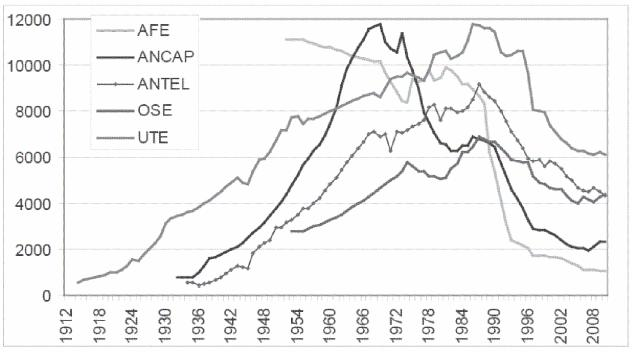
\includegraphics{imagenes/fig5.jpg}
\caption{Evolución del número de funcionarios en cinco empresas públicas
(1912-2010).}
\end{figure}

Fuente: \citet{Bertino2012}, gráfico 4.

En los 90, predominaban en la región y en el resto del mundo las
propuestas de reformas orientadas al mercado, con el objetivo de
promover la eficiencia económica y el crecimiento. \citet{Forteza2003}
mencionan las políticas desarrolladas en esos años, con el objetivo de
promover la competencia, la apertura comercial, la privatización y el
desmantelamiento de los monopolios de las empresas públicas. Estas
medidas se planteaban bajo el supuesto que las mismas permitirían
generar mayores niveles de competencia, promover la inversión privada y
el progreso técnico y, en consecuencia, una asignación de recursos más
eficiente.

Asimismo, sostienen que los cambios tecnológicos, observados hacia fines
del siglo pasado, habían modificado la vieja concepción de que los
servicios públicos constituían monopolios naturales y, por tanto,
surgían propuestas de incentivar la competencia en dichos mercados con
el objetivo de reducir los costos para el consumidor final y,
fundamentalmente, para las empresas, lo que mejoraría la competitividad
de la economía.

Bajo estos supuestos, en la mayoría de los países de la región se
produjeron procesos o intentos de privatización de empresas estatales
que operaban en diferentes mercados, entre ellas las empresas de
servicios públicos. Según \citet{Bergara2005} los intentos de
privatización en la región tuvieron resultados parciales, observándose
una mayor aceptación en aquellos países donde la provisión estatal de
servicios públicos era sumamente deficiente.

Si bien en Uruguay las empresas públicas tenían algunas características
que las diferenciaban de lo que sucedía en otros países de la región (no
tenían grandes déficits y realizaban una cobertura del servicio bastante
amplia) las mismas presentaban deficiencias en lo relativo a la calidad
del servicio que prestaban \citep{Forteza2003}.

En este marco el gobierno de la época intenta aplicar reformas
orientadas al mercado, principalmente, en los sectores de energía
eléctrica, comunicaciones y combustibles. La finalidad de las reformas
era incrementar la competencia en los mercados de los servicios públicos
y privatizar, parcialmente, a las empresas públicas. Para ello se
propusieron leyes que modificaban el alcance de los monopolios de las
empresas públicas y posibilitaban la incorporación de capitales privados
\citep{Bergara2005}.

La \href{http://www.parlamento.gub.uy/leyes/ley16211.htm}{Ley
No.~16.211} de Empresas Públicas, aprobada por el Parlamento en 1992,
establecía el cierre de algunas empresas públicas (ILPE - pesca), la
privatización de otras (PLUNA - aviación) y la venta parcial de la
Administración Nacional de Telecomunicaciones (ANTEL), y representó el
primer intento por realizar reformas orientadas al mercado. Este intento
fracasa ante el referéndum que provocó la derogación de algunos
artículos de esta ley (principalmente los referidos a ANTEL). Ello llevó
a profundizar la política de mejora y búsqueda de eficiencia de las
empresas públicas, en el marco de cierto consenso sobre la utilización
de los beneficios de estas empresas como fuente adicional de ingresos
fiscales \citep{Bergara2005}.

\citet{Forteza2003}, a su vez, señalan que una vez cerrada la
posibilidad de las privatizaciones, la agenda de la reforma de los
servicios públicos se reorientó hacia la remoción de los monopolios a
través de la desregulación, la competencia y la asociación con privados
en nuevos emprendimientos. La
\href{https://www.impo.com.uy/bases/leyes/16832-1997}{Ley No.~16.832} de
Marco Regulatorio del Sector Eléctrico (1997) reiteraba la posibilidad
de competencia en la generación de energía tal como lo establecía la Ley
Nacional de Electricidad del año 1977
(\href{https://www.impo.com.uy/bases/decretos-ley/14694-1977}{Decreto
Ley No.~14.694}), mientras mantiene a la Administración Nacional de
Usinas y Transmisiones Eléctricas (UTE) como empresa monopólica estatal
en la transmisión y distribución de la energía eléctrica.

Con la regulación de esta ley se establece, en el año 2000, la Unidad
Reguladora de la Energía Eléctrica (UREE) la que comienza a funcionar en
el año 2001 cuando se le asigna presupuesto específico. Poco después, en
el año 2002 se modifican sus cometidos, creándose la Unidad Reguladora
de los Servicios de Energía y Agua (URSEA).

En el sector de comunicaciones el proceso de reformas se inicia cuando
se aprueba la nueva carta orgánica de ANTEL, que la modifica
sustancialmente, y se crea la Unidad Reguladora de los Servicios de
Comunicación (URSEC), en el año 2001. Esta legislación permitía la
privatización de la división de telefonía celular de ANTEL, y abría la
competencia en varios segmentos. Sin embargo, en 2002 los artículos
fundamentales de esta ley se derogan, permitiendo en el breve período de
aplicación la incorporación de competencia en el mercado de telefonía
celular y de llamadas internacionales.

El último intento, en este proceso de apertura al mercado, fue la
autorización a la Administración Nacional de Combustibles, Alcohol y
Portland (ANCAP) para asociarse con privados en la refinación de
petróleo y venta de productos refinados por un período de 30 años, y la
liberalización de la importación de petróleo a partir de 2006. Esta
norma también fue derogada por plebiscito en 2003.

Según \citet{Bergara2005} las reformas orientadas al mercado fueron de
alcance limitado y variaron considerablemente en función del sector de
actividad. Aquellas reformas que requerían cambios en el marco legal
tuvieron problemas serios. En algunos casos los plebiscitos impidieron
su aplicación (comunicaciones, combustibles), mientras que en otros
-energía- se demoró su puesta en funcionamiento. Por su parte, en las
reformas que solo requerían la implementación de medidas
administrativas, la participación de los privados se promovió a través
de la concesión de los monopolios locales, tal el caso de las
concesiones en los servicios de agua y saneamiento (en escala reducida)
así como en la infraestructura de carreteras, puertos y aeropuertos, y
en el mercado de los seguros y el correo.

Por su parte, \citet{Forteza2003} señalan que como resultado del
plebiscito de 1992 sobre las empresas públicas, los sectores reformistas
cambiaron sus propuestas hacia el fortalecimiento de estas empresas. En
este marco se observa, a vía de ejemplo: (i) la reestructura, entre 1995
y 2000, de UTE a través de cuantiosas inversiones; (ii) la mejora de
ANCAP, invirtiendo en la ampliación de la capacidad de su refinería, la
compra de una compañía distribuidora en Argentina, y la transferencia de
la distribución de productos derivados del petróleo en Uruguay a una
empresa privada (de su propiedad); (iii) la expansión de las actividades
de ANTEL hacia la telefonía celular.

A comienzos del siglo XXI y como consecuencia de la mejora en la gestión
de las empresas estatales en energía y telecomunicaciones, tanto UTE
como ANTEL presentaban indicadores considerablemente mejores a los de
las empresas estatales en países en desarrollo, y habían aumentado
considerablemente las utilidades vertidas al fisco de forma permanente
\citep{Bergara2005}.

Estos cambios fueron acompañados por transformaciones en la gestión de
estas empresas. \citet{Oria2008} señala que las empresas pasaron de
centrar su atención en los problemas internos a centrarla en el cliente
y su posicionamiento en el mercado. Es decir, el paradigma volvió a
centrar a las empresas públicas como empresas que intervienen en
mercados con clientes y, a veces, competidores.

Luego de una década de diversos intentos de reformas de los servicios
públicos, \citet{Bergara2005} sostienen que en Uruguay este proceso ha
sido relativamente volátil ya que las reformas que pasaron por el
Parlamento fueron, en su mayoría, derogadas por la vía de los
referéndum, mientras que las que no requerían de ley -como el sector
eléctrico- sufrieron retrasos importantes en su implementación.
Atribuyen este resultado a diversos factores: (i) preferencia de lo
público frente a lo privado por parte de la mayoría de la población, lo
que determina la alta valoración que esta tiene sobre las empresas
públicas; (ii) preferencias políticas no muy divergentes con relación a
la propiedad de las empresas de servicios públicos, donde la
privatización masiva de las empresas públicas no era una propuesta
predominante; y (iii) razones pragmáticas de quienes gobiernan que
requieren de las ganancias de las empresas para lograr cerrar la brecha
fiscal.

Asimismo, señalan que la consolidación de las empresas públicas como
financiador de las cuentas públicas ha sido un factor determinante en el
desarrollo de su reforma estructural. Ante situaciones problemáticas de
déficit fiscal recurrir a recursos provenientes de estas empresas tiene
ventajas frente a otras formas de financiamiento (impuestos,
endeudamiento), ya que no requiere aprobación parlamentaria. Estos
factores jugaron en contra del interés de promover mayor competencia en
los sectores de servicios públicos.

El debate en torno a la reforma de los servicios públicos tuvo amplia
difusión y participación, fundamentalmente en el ámbito político. El
documento elaborado en el marco del proyecto Agenda Uruguay y publicado
en 2001 ``Servicios públicos: aportes hacia una política de Estado''
\citep{CIIIPUPAZ2001} trata de recoger diferentes concepciones respecto
a esta temática. Los artículos señalan la necesidad de una política de
Estado con el objetivo de mejorar la calidad de los servicios públicos,
reducir las tarifas que pagan los contribuyentes y lograr el mejor
desarrollo económico y social para Uruguay. La mayoría de las propuestas
combinan la introducción de una mayor competencia en estos mercados con
la incorporación de la regulación de los mismos.

A ese respecto \citet{Bergara2001} sostiene que ``(\ldots) en los
albores del nuevo milenio, el Estado del bienestar debe seguir
existiendo, pero ha cambiado las formas con las que pretende cumplir sus
fines. Este nuevo Estado del bienestar distingue de manera sana su rol
de regulador, de proveedor de servicios y de compensador de
desigualdades, buscando ser el garante de los intereses de los
ciudadanos. Los nuevos códigos son mercados competitivos, regulación
fuerte que evite abusos monopólicos y promueva la competencia,
participación más directa de los usuarios y subsidios explícitos que
amplíen el acceso a los servicios básicos de las capas sociales más
excluidas''. \citet{Mederos2001} propone transitar hacia una
``competencia regulada'' reconociendo que existen fallas de mercado que
impiden la libre competencia y por ende la maximización de los
beneficios sociales.

Finalmente, mientras se procesaba este debate en diferentes foros, se
aprobó la modificación constitucional que establece que el agua es
``parte del dominio público'' y por ende su provisión privada resulta
ilegal. La disposición constitucional, aprobada en 2004, llevó a la
nacionalización de la provisión de agua y saneamiento en aquellas
localizaciones donde el servicio se proveía por parte de firmas
privadas, con anterioridad a la existencia de la empresa estatal Obras
Sanitarias del Estado (OSE), o donde el mismo se había privatizado o
entregado en concesión en los 90.

\hypertarget{panorama-actual-de-las-empresas-puxfablicas-en-uruguay}{%
\section{Panorama Actual de las Empresas Públicas en
Uruguay}\label{panorama-actual-de-las-empresas-puxfablicas-en-uruguay}}

Las actuales empresas públicas difieren según el sector de actividad en
el que operan. En este trabajo, se consideran las empresas públicas de
combustibles (ANCAP), electricidad (UTE), telefonía (ANTEL) y agua
(OSE). Las restantes empresas públicas no se analizan debido a que la
lógica de sus mercados y su consiguiente regulación es diferente (Banco
de Seguros del Estado (BSE), BROU, sector financiero), porque tienen una
baja actividad empresarial (AFE, ferrocarriles), o porque la prestación
del servicio está dispersa entre diversos operadores (saneamiento).

En términos generales, se puede señalar que las tarifas que han cobrado
históricamente estas empresas por sus servicios han estado por debajo de
la inflación, con excepción de los combustibles líquidos (gasolinas) y
la energía eléctrica. En el gráfico @ref(fig:fig3) se puede observar que
las tarifas de gas, teléfono y agua evolucionan por debajo de la
inflación promedio anual, mientras que la energía eléctrica lo hace
fundamentalmente por encima.

\begin{figure}
\centering
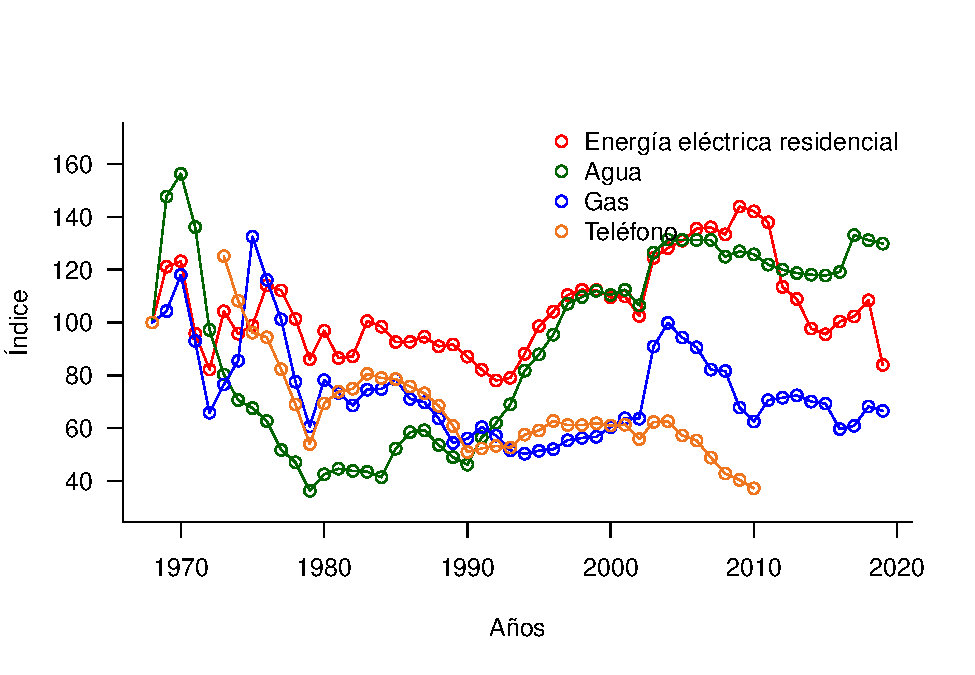
\includegraphics{Regulacion_files/figure-latex/fig3-1.pdf}
\caption{Evolución real de tarifas públicas, 1968-2000 (Base 1968=100)}
\end{figure}

Fuente: elaboración propia con base en datos del INE.

Por su parte, las tarifas de las gasolinas se disparan a partir del año
1973, con motivo de la crisis del petróleo, y convergen nuevamente a la
inflación a partir de la década de los noventa (gráfico
@ref(fig:fig4)).\\

\begin{figure}
\centering
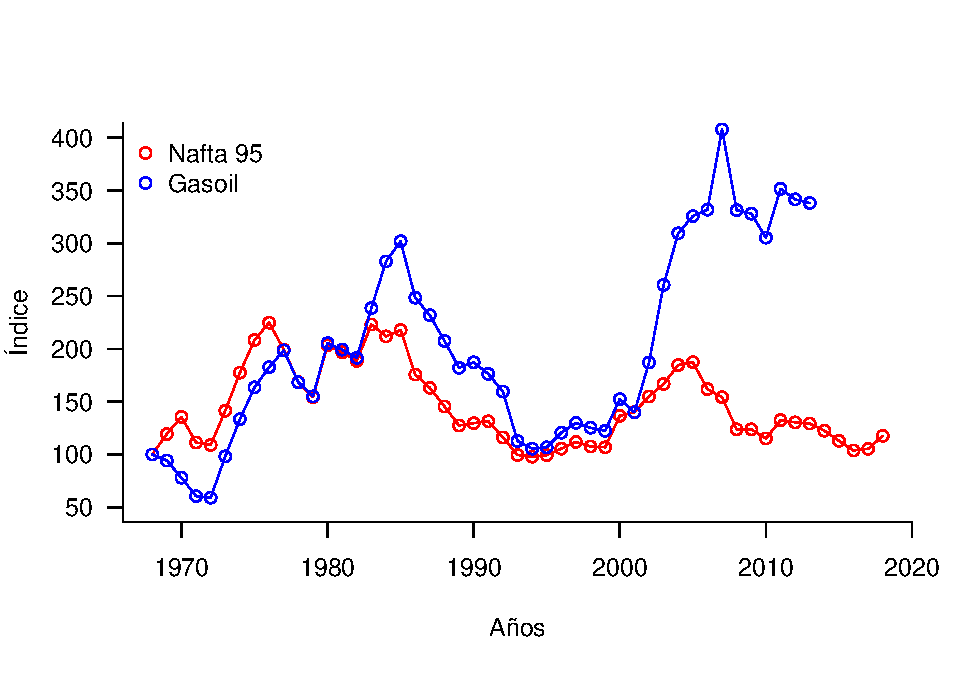
\includegraphics{Regulacion_files/figure-latex/fig4-1.pdf}
\caption{Evolución real del precio de las gasolinas, 1968-2019 (Base
1968=100)}
\end{figure}

Fuente: elaboración propia con base en datos del INE y
\href{https://www.ancap.com.uy/innovaportal/v/6088/1/innova.front/historico-precio-combustibles.html}{ANCAP}.

\hypertarget{el-mercado-de-las-telecomunicaciones}{%
\subsection{El mercado de las
telecomunicaciones}\label{el-mercado-de-las-telecomunicaciones}}

En el mercado de la telefonía, ANTEL tiene el monopolio de la telefonía
fija, compite con dos empresas privadas en telefonía celular, y existe
un monopolio de hecho en la transmisión de datos. Uruguay tuvo,
históricamente las tarifas de telefonía fija más altas de la región, al
tiempo que la conectividad a internet estuvo limitada durante muchos
años, lo que impactaba en la competitividad de las empresas que utilizan
este medio como insumo para sus servicios.

Desde el año 2014 ANTEL comenzó la instalación de fibra óptica al hogar
lo que ha permitido mejorar la conectividad a internet, y también
permitiría suplantar la tecnología de telefonía básica ya que ambas
utilizan la misma plataforma. Si bien aún conviven ambas plataformas,
este cambio tecnológico hizo crecer a Uruguay en los rankings
internacionales. En el cuadro @ref(tab:cuadro6) se presentan diversos
indicadores del sector de telecomunicaciones a nivel internacional.

\begin{longtable}[]{@{}lrrrrr@{}}
\caption{Indicadores del sector telecomunicaciones para países
seleccionados de América}\tabularnewline
\toprule
País & Teléfonos c/100 habitantes & Celulares c/100 habitantes & Hogares
con acceso a internet (\%) & Precio banda ancha (U\$S PPC) & Precio
banda ancha (U\$S PPC\tabularnewline
\midrule
\endfirsthead
\toprule
País & Teléfonos c/100 habitantes & Celulares c/100 habitantes & Hogares
con acceso a internet (\%) & Precio banda ancha (U\$S PPC) & Precio
banda ancha (U\$S PPC\tabularnewline
\midrule
\endhead
Argentina & 22 & 142 & 81 & NA & NA\tabularnewline
Bolivia & 8 & 99 & 32 & 51 & 21\tabularnewline
Brasil & 20 & 113 & 61 & 25 & 16\tabularnewline
Chile & 18 & 128 & 89 & 46 & 18\tabularnewline
Colombia & 14 & 127 & 50 & 42 & 28\tabularnewline
Ecuador & 15 & 84 & 37 & 39 & 25\tabularnewline
México & 16 & 89 & 51 & 10 & 12\tabularnewline
Paraguay & 4 & 110 & 20 & 50 & 13\tabularnewline
Perú & 10 & 121 & 28 & 28 & 20\tabularnewline
Uruguay & 33 & 148 & 64 & 0 & 22\tabularnewline
Venezuela & 19 & 77 & 34 & NA & NA\tabularnewline
EUA & 37 & 123 & 87 & 50 & 44\tabularnewline
Canadá & 40 & 86 & 91 & 25 & 25\tabularnewline
\bottomrule
\end{longtable}

Fuente: elaboración propia con base en Measuring the Information Society
de la International Telecomumunication Union 2018
\href{https://www.itu.int/en/ITU-D/Statistics/Documents/publications/misr2018/MISR-2018-Vol-1-E.pdf}{vol.~1}
datos de precios (tablas 4.1, 4.6 y ) y
\href{https://www.itu.int/en/ITU-D/Statistics/Documents/publications/misr2018/MISR-2018-Vol-2-E.pdf}{vol.~2},
datos de acceso.

Los datos destacan lo bien posicionado que está el país en
telecomunicaciones respecto a sus pares en América Latina, e inclusive
tomando como referencia Canadá y Estados Unidos (EUA). Ello es el
resultado de la fuerte competencia a la que está sometida la empresa
pública en los distintos mercados (telefonía celular y transmisión de
datos), lo que la ha llevado a mejorar notoriamente los indicadores de
desempeño. En lo que refiere a banda ancha, donde ANTEL está
desarrollando el plan de instalación de fibra óptica al hogar, se
apreciaba inicialmente una fuerte competencia por el mercado.

Es de hacer notar que en esta competencia la empresa pública ha recibido
ayuda del Estado, ya sea por acción u omisión, dado que los competidores
privados no han podido obtener licencias para instalar tendido de fibra
óptica. Sin embargo, para que ANTEL pueda sostener estos buenos
resultados, es necesario retomar la competencia en este sector que en la
actualidad se encuentra acotada. Cuando la competencia \emph{por el
mercado} se alcance, habrá que retomar la competencia \emph{en el
mercado} para que la eficiencia de la empresa no se deteriore. En el
cuadro @ref(tab:cuadro7) se presenta un panorama del sector de las
telecomunicaciones en Uruguay.

\begin{longtable}[]{@{}rrrrrr@{}}
\caption{Indicadores seleccionados del mercado de telecomunicaciones en
Uruguay (2008-2018)}\tabularnewline
\toprule
Año & Numero teléfonos celulares (miles) & Numero teléfonos fijos
(residenciales, miles) & Minutos tráfico celular (millones) & Cómputos
telefonía fija (millones) & Servicios banda ancha (miles)\tabularnewline
\midrule
\endfirsthead
\toprule
Año & Numero teléfonos celulares (miles) & Numero teléfonos fijos
(residenciales, miles) & Minutos tráfico celular (millones) & Cómputos
telefonía fija (millones) & Servicios banda ancha (miles)\tabularnewline
\midrule
\endhead
2008 & 3508 & NA & 2669 & 3401 & 244\tabularnewline
2009 & 4112 & NA & 3818 & 3106 & 317\tabularnewline
2010 & 4437 & 775 & 4812 & 2804 & 383\tabularnewline
2011 & 4575 & 796 & 5276 & 2519 & 473\tabularnewline
2012 & 4995 & 821 & 5886 & 2355 & 581\tabularnewline
2013 & 5268 & 856 & 6181 & 2157 & 737\tabularnewline
2014 & 5497 & 886 & 6184 & 1979 & 840\tabularnewline
2015 & 5495 & 909 & 6281 & 1757 & 901\tabularnewline
2016 & 5420 & 918 & 5846 & 1559 & 922\tabularnewline
2017 & 5391 & 934 & 5278 & 1304 & 950\tabularnewline
2018 & 5437 & 951 & 4683 & 1094 & 977\tabularnewline
\bottomrule
\end{longtable}

Fuente: elaboración propia con base en datos
\href{https://www.gub.uy/unidad-reguladora-servicios-comunicaciones/sites/unidad-reguladora-servicios-comunicaciones/files/2019-10/Informe\%20Telecomunicaciones\%20a\%20diciembre\%20de\%202018\%20corregido.pdf}{URSEC}.

Los resultados del sector de telefonía celular demuestran también como
la competencia funciona como incentivo a la búsqueda de mejores
resultados (tarifas adecuadas y expansión del servicio). Este proceso
comenzó con el ingreso de América Móvil en 2004, lo que provocó una
fuerte expansión en el mercado. Ese incremento también se observa en el
uso de celulares, con una duplicación del número de minutos entre 2008 y
2013. En el año 2015 se observa un máximo y luego una fuerte caída en el
número de minutos.

Por su parte, la telefonía fija presenta un aumento sostenido en el
número de lineas, quizá explicado por el incremento en el número de
servicios de banda ancha fija, que necesita disponer de un teléfono fijo
para obtener el servicio. Esto se verifica al observar el incremento en
el número de servicios de banda ancha que se cuadriplica entre 2008 y
2018, y la sostenida caída en el número de cómputos de telefonía fija
que determina, que en 2018, este sea menos de un tercio del valor de
2008. La telefonía fija es un mercado que tiende a ser sustituido por la
telefonía celular y por la transmisión de datos.

Por último, debe señalarse que ANTEL opera fundamentalmente bajo la
figura de empresa pública, pero posee cuatro empresas de propiedad
pública que operan en el ámbito del derecho privado, con el objetivo de
dar funciones de apoyo no sustantivas.

Estas empresas son: - ITC S.A. que tiene por objeto brindar servicios de
asesoramiento y asistencia en el área de telecomunicaciones, tecnología
de la información y de la gestión tanto en el país como en el exterior,
de la cual ANTEL es propietaria del 99,924\% de su capital; - HG S.A.
que se dedica a la realización de proyectos de integración tecnológica y
de servicios, asociados al desarrollo y operación de sitios web y
portales siendo propiedad de ANTEL el 99,8026\% de su capital; - ACCESA
S.A. cuyo objeto principal es brindar servicios de Call Center y Contact
Center, procesamiento de información, datos y contenidos mediante
sistemas de telecomunicaciones y tecnología de la información, siendo
ANTEL propietaria del 95,74\% del capital; y - ANTEL USA Inc.~con sede
en Estados Unidos cuyo cometido es proveer servicios de interconexión de
datos (IP) desde ese país a compañías de telecomunicaciones en América
Latina, siendo ANTEL propietaria del 100\% del capital.

\hypertarget{mercado-de-combustibles-glp-y-gas}{%
\subsection{Mercado de combustibles, GLP y
gas}\label{mercado-de-combustibles-glp-y-gas}}

ANCAP tiene el monopolio de la importación y refinamiento de
combustibles desde su creación en el año 1931. Los combustibles se
producen en una única refinaría con petróleo importado. En el mercado de
distribución de combustibles operan tres empresas: DUCSA, 99\% propiedad
de ANCAP; ESSO y Petrobras. Asimismo, las estaciones que venden el
combustible al público son privadas y operan bajo la marca de algunos de
los distribuidores. \footnote{Existen unas 448 estaciones de servicio en
  el país, el 60\% con bandera ANCAP \citep{URSEA2013}.}

Por su parte el suministro de combustibles a las aeronaves, en la
terminal del aeropuerto, lo realiza Talobras empresa en la que ANCAP,
Orodone S.A. y Petrobras comparten el capital. A los efectos de observar
la evolución del precio de la gasolina y compararlo con otros países, en
el gráfico @ref(fig:fig6) se presenta el precio de la gasolina para los
países del MERCOSUR, NAFTA y otros de Sudamérica, para los años en que
la información estaba disponible.

\begin{figure}
\centering
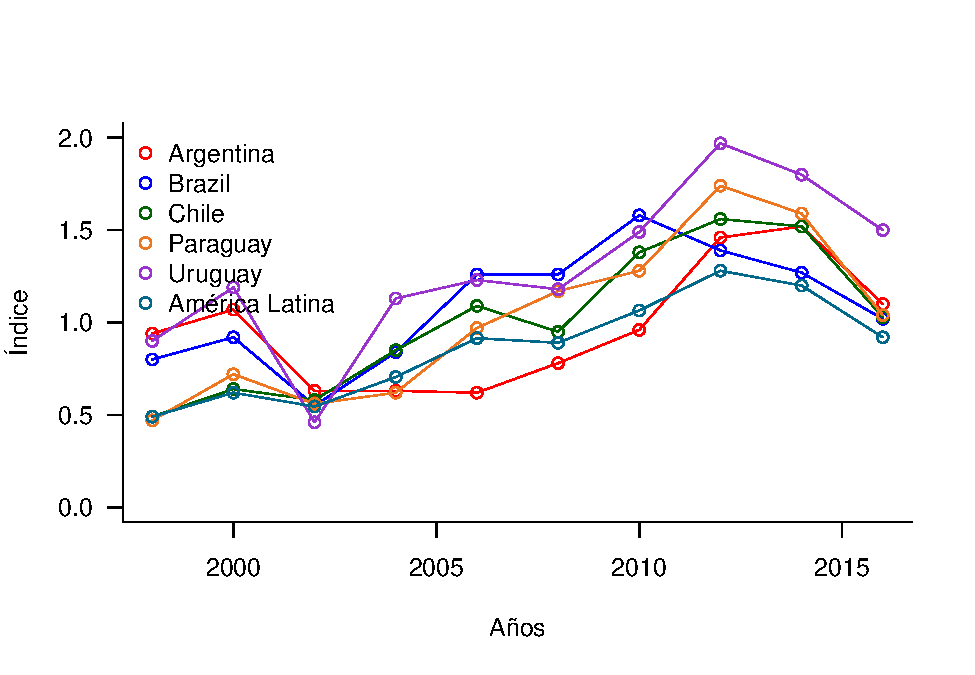
\includegraphics{Regulacion_files/figure-latex/fig6-1.pdf}
\caption{Precio de la gasolina para países de América Latina (en
dólares)}
\end{figure}

Fuente: World Development Indicators, Banco Mundial.

Como se puede observar, el precio de la gasolina en Uruguay está entre
los más caros de la región. Este resultado, a diferencia del anterior
referido a las telecomunicaciones, tiene diversas consideraciones. En
efecto, Uruguay no es un país que tenga petróleo, como lo es Venezuela o
Ecuador, y por tanto debe importar el crudo que refina. Por otra parte,
el monopolio que rige en Uruguay, sometido a una regulación laxa -la
propia empresa fija sus precios-, influye en su eficiencia.

El GLP se obtiene del refinamiento de petróleo en la planta de La Teja
de ANCAP. Una vez producido se transfiere a la planta de despacho de La
Tablada y de allí a las dos plantas de envasado: la de GASUR, que envasa
para las empresas Riogas y Acodike, y la planta de Megal. En la
distribución minorista operan cuatro empresas: Acodike, Riogas, Megal y
DUCSA (sociedad anónima propiedad de ANCAP en 99\% del capital). El
precio máximo al consumidor final lo fija el Poder Ejecutivo, a
iniciativa de ANCAP.

ANCAP es accionista en más de una docena de sociedades anónimas a través
de las cuales diversifica sus negocios. Estas empresas se concentran en
cemento, gas natural, alcoholes y bebidas alcohólicas, agroindustrias,
exploración y producción de petróleo, negocios en Argentina y asistencia
técnica.

La comercialización de los cementos ANCAP se realiza a través de la
firma Cementos del Plata S.A. en la cual ANCAP posee el 99,25\% del
paquete accionario. Vinculado al negocio de cementos, ANCAP también es
propietaria de PAMACOR S.A. empresa dedicada a la prospección,
exploración, explotación, comercialización, importación y exportación de
recursos minerales y productos derivados.

En el sector de gas natural ANCAP, a través de Gaseoducto Cruz del Sur
S.A., donde participa con el 20\% del capital accionario junto a firmas
extranjeras, opera en el transporte de este combustible desde Argentina.
Por su parte, mediante la empresa CONECTA, propiedad de ANCAP (45\% del
capital accionario) y Petrobras Uruguay, participa en la distribución
interna de gas por cañería (excepto Montevideo); mientras que Petrobras
Uruguay tiene la distribución en Montevideo. Asimismo, ANCAP participa
junto a UTE en el desarrollo de la Planta Regasificadora para recepción,
almacenamiento y regasificación de gas natural licuado, mediante la
empresa conjunta Gas Sayago S.A.

En GLP, ANCAP (40\%) participa con empresas privadas (Acodike y Riogas)
en Gasur Uruguay S.A. para la venta y distribución, en sus diferentes
modalidades, de propano industrial a granel y gases canalizados, a
clientes que cuenten con instalaciones adecuadas para su consumo.

En negocios agroindustriales, ALUR S.A., 97\% propiedad de ANCAP, es el
principal productor de biocombustibles, azúcar y harinas proteicas, así
como de alcoholes. En el sector de alcoholes también opera la Compañía
ANCAP de Bebidas y Alcoholes, S.A. (CABA) que produce, compra,
comercializa y distribuye alcoholes y bebidas alcohólicas, entre otros.

Por último, ANCAP maneja sus negocios en Argentina a través de dos
subsidiarias. Petrouruguay S.A., que desarrolla actividades de
exploración, producción y comercialización de gas y petróleo, en cuyo
capital ANCAP participa con el 99,84\% directamente y a través de ANCSOL
S.A. (una SAFI 100\% propiedad de ANCAP). Por su parte, Carboclor S.A.
propiedad de ANCSOL S.A. y de Petrouruguay S.A., se dedica
principalmente a la producción de solventes y alcoholes a partir de
corrientes de refinerías de petróleo.

En los últimos años, ANCAP se embarcó en una serie de inversiones para
sus diferentes divisiones, muchas de las cuales se han visto
cuestionadas por el sobre costo en la ejecución de las obras. Asimismo,
los resultados económicos de la empresa han devenido negativos, lo que
ha determinado la necesidad de una sustantiva capitalización de la
empresa.

\hypertarget{energuxeda-eluxe9ctrica}{%
\subsection{Energía eléctrica}\label{energuxeda-eluxe9ctrica}}

El sector eléctrico es el más complejos de los sectores objeto de
estudio. Tiene tres componentes: generación, transmisión y distribución.
En la generación operan distintos agentes que producen energía eléctrica
con base en distintas fuentes (hidroeléctrica, solar, biomasa, eólica,
etc.). En 2019, el 55\% de la generación eléctrica correspondía a
fuentes hidráulica, 34\% a eólica, 6\% a biomasa, 3\% a fotovoltaica y
2\% térmica.

En la transmisión eléctrica, típico segmento de monopolio natural, UTE
tiene el monopolio legal de la actividad al igual que en la
distribución. Lo interesantes es que esta empresa pública compite en los
mercados internacionales, en la medida en que vende energía eléctrica a
los países vecinos, en particular a Argentina.

La eficiencia en el sector depende de la posibilidad de utilizar la
fuente más barata para la generación de energía, y esta es la
hidroeléctrica. Sin embargo, ello depende de factores no controlables
por la empresa como el clima. Asimismo, el país ha tomado importantes
decisiones para la instalación de fuentes alternativas de energía
(parques eólicos principalmente), los que se encuentran en etapa de
desarrollo.

Si bien UTE es el principal agente de suministro de energía eléctrica,
es posible para los grandes consumidores contratar directamente con las
empresas generadoras y utilizar la red de transmisión de UTE para que
lleve la energía eléctrica contratada. El marco jurídico que permite la
efectivización de estos contratos se encuentra reglamentado y operativo,
sin embargo, a la fecha, no se han registrado contratos entre
particulares y todos los grandes consumidores continúan contratando
directamente con UTE.

En este sector resulta difícil establecer un indicador que permita
comparar la eficiencia relativa de la empresa con otros actores de la
región. Los datos disponibles, sistematizados a nivel internacional,
refieren principalmente a la cobertura de energía eléctrica a los
hogares. Este indicador puede ser considerado un resultado de eficacia
(acceso universal a la red de energía eléctrica) desde el punto de vista
social, sin embargo nada dice de la eficiencia de la empresa. Otro
indicador, como el precio del servicio, depende de factores externos a
la empresa, como el clima, cuando la generación se basa en energía
hidroeléctrica y tampoco nos permite comparar eficiencia relativa. Solo
en los casos en que la mayor parte de la generación se base en fuentes
alternativas a la hidroeléctrica, las mismas serían controlables por la
empresa y su operativa puede tener impactos sobre los costos de
generación, haciendo que el precio pueda servir como variable de
comparación.

\hypertarget{agua-potable}{%
\subsection{Agua potable}\label{agua-potable}}

Como fuera señalado, desde el año 2004 la producción y distribución de
agua potable se encuentra bajo monopolio del Estado por norma
constitucional. Por tanto, OSE actúa como monopolista en este mercado.
El hecho de que con anterioridad a esa fecha existieran otras empresas
prestadoras del servicio de agua potable no implicaba que existiera
competencia entre ellas, ya que dado un mercado geográfico, el servicio
de agua potable es un monopolio natural.

Al igual que en los casos anteriores, existe una variedad de dimensiones
sobre las cuales se puede comparar el desempeño de la empresa, por
ejemplo, agua facturada en el total de agua producida, número de roturas
en los caños, horas sin servicio de agua potable, etc. Sin embargo, para
tener información comparable, se toma aquella sistematizada por el Banco
Mundial sobre conexión a la red, tanto en las ciudades como en el medio
rural de algunos países de América, la que se presenta en el cuadro 3.

De manera general, puede observarse que el desempeño de OSE, medido en
términos de cobertura, ha mejorado sustancialmente entre 1990 y 2012 al
igual que en el resto de los países de la región. Asimismo,
\citet{Borraz2013} demuestran que la estatización del servicio, producto
de la reforma constitucional, se tradujo en un incremento en el acceso a
la red de agua potable y en la mejora en la calidad del agua.

\begin{longtable}[]{@{}ccccc@{}}
\caption{Tasa de cobertura del sistema de agua potable. Países
seleccionados. (en porcentaje}\tabularnewline
\toprule
País & Rural, año 1990 & Rural, año 2018 & Urbana, año 1990 & Urbana,
año 2018\tabularnewline
\midrule
\endfirsthead
\toprule
País & Rural, año 1990 & Rural, año 2018 & Urbana, año 1990 & Urbana,
año 2018\tabularnewline
\midrule
\endhead
Argentina & 69 & 93 & 97 & 99\tabularnewline
Bolivia & 41 & 78 & 91 & 99\tabularnewline
Brasil & 68 & 90 & 96 & 99\tabularnewline
Chile & 48 & 99 & 99 & 99\tabularnewline
Colombia & 69 & 86 & 98 & 99\tabularnewline
Ecuador & 61 & 83 & 84 & 99\tabularnewline
Paraguay & 24 & 99 & 83 & 99\tabularnewline
Perú & 44 & 76 & 88 & 96\tabularnewline
Uruguay & 75 & 95 & 98 & 99\tabularnewline
Venezuela & 71 & NA & 93 & NA\tabularnewline
EUA & 94 & 97 & 100 & 99\tabularnewline
Canadá & 99 & 99 & 100 & 100\tabularnewline
\bottomrule
\end{longtable}

Fuente: World Development Indicators, Banco Mundial.

OSE tiene participación en tres empresas privadas: - Aguasur (Manantial
Dorado S.A.), en la que posee el 95\% de las acciones, cuyo cometido es
la construcción, remodelación, y/o mantenimiento de soluciones
estructurales para el tratamiento de líquidos residuales, el
abastecimiento de agua potable y/o actividades vinculadas a la misma. -
Aguas de la Costa S.A., donde OSE posee el 60\% del capital accionario y
cuya actividad principal es dar cumplimiento al contrato de obra pública
para el suministro de agua potable a una zona del Departamento de
Maldonado. - Consorcio Canario Ciudad de la Costa S.A. cuyo cometido es
la administración de las contrataciones y gestión de las actividades
relativas al Programa Integrado de Saneamiento, Drenaje Pluvial y
Vialidad en Ciudad de la Costa, Departamento de Canelones, siendo OSE y
la Intendencia de Canelones titulares de las acciones por partes
iguales.

\hypertarget{el-marco-institucional-de-las-empresas-puxfablicas-en-uruguay}{%
\section{El Marco Institucional de las Empresas Públicas en
Uruguay}\label{el-marco-institucional-de-las-empresas-puxfablicas-en-uruguay}}

La importancia que la sociedad -o el sistema político- le ha asignado
tradicionalmente a las empresas públicas en Uruguay, se manifiesta en el
hecho de que las actividades industriales y comerciales del Estado
tienen una figura específica en la Constitución de la República.

Las empresas propiedad del Estado, antes de 1934, operaban bajo el mismo
régimen jurídico que las empresas privadas. La Constitución de ese año
crea una nueva figura jurídica para ``los diversos servicios que
constituyen el dominio industrial y comercial del Estado (\ldots)'', la
que se fue modificando con las siguientes reformas constitucionales.

A partir de la Constitución de 1934, \footnote{Véase la
  \href{https://legislativo.parlamento.gub.uy/temporales/2680947.HTML}{Constitución
  de 1934} artículo 181.} esta figura jurídica adopta dos formas
posibles: Entes Autónomos y Servicios Descentralizados. Su objetivo fue
permitir dotar a las empresas públicas de mayor grado de autonomía que a
otras instituciones de la administración pública.

Esta movida estratégica, en los hechos, impuso un límite a la
discrecionalidad en la que operan las empresas públicas en Uruguay. En
efecto, la forma jurídica que les hubiera permitido a estas empresas
alcanzar la mayor independencia posible era que se hubiera mantenido
bajo el régimen de sociedades anónimas y se guiaran, en ese momento, por
el Código de Comercio, o por la Ley de Sociedades Comerciales, en la
actualidad. La Constitución de 1918, sacó a las empresas de la órbita
privada y las puso bajo controles similares al resto de los organismos
del Estado.

En la actualidad, la sección XI ``De los Entes Autónomos y de los
Servicios Descentralizados'' (artículos 185 a 201) de la Constitución,
constituye el marco legal general que ampara la creación y
funcionamiento de los Entes Industriales o Comerciales del Estado. En
esta sección de la Constitución se establecen las condiciones para la
creación o supresión de Entes Autónomos (artículo 189), así como el
marco de actuación de las empresas públicas: - Designación de
autoridades y las características de las mismas en cuanto a duración en
sus funciones, cese o inhibiciones (artículos 185 y 187). - Condiciones
relativas a posible participación de capitales privados, limitando su
participación y representación a un porcentaje menor al del Estado
(artículo 188). - Restricción de actividades a las establecidas por ley
(artículo 190). - Obligación de presentar estados financieros con el
visto bueno del Tribunal de Cuentas (artículo 191).

Por otra parte, en la Constitución también se establecen otras
disposiciones que afectan el funcionamiento de las empresas públicas.
Entre ellos merecen señalarse, los siguientes:

\begin{enumerate}
\def\labelenumi{\arabic{enumi}.}
\item
  El establecimiento de monopolios (a favor del Estado) que requiere la
  mayoría absoluta de los votos del total de componentes de la Asamblea
  General (artículo 85, inciso 17).
\item
  Las disposiciones sobre los regímenes relativos a los funcionarios de
  estas empresas, que se regirán por un Estatuto que, proyectado por las
  mismas, deberá ser aprobado por el Poder Ejecutivo, en el caso de los
  Entes Autónomos (artículo 63). Por su parte, si la empresa pública
  tiene el carácter de servicio descentralizado (OSE, ANTEL) el Estatuto
  debe ser aprobado por ley (artículo 59). Asimismo, establece que la
  ley deberá crear el Servicio Civil de la Administración Central, Entes
  Autónomos y Servicios Descentralizados que tendrá injerencia en esta
  materia sobre todos los órganos del Estado.
\item
  Intervención preventiva de los gastos y pagos, y en todo lo referente
  a su gestión financiera, por parte del Tribunal de Cuentas de la
  República (artículo 211), el que ejercerá además la superintendencia
  sobre las oficinas de contabilidad, recaudación y pagos de las
  empresas públicas (artículo 212).
\item
  Las disposiciones relativas a la Hacienda Pública donde se indican los
  mecanismos referidos a la elaboración de los presupuestos de los Entes
  Industriales o Comerciales del Estado (artículo 220), su aprobación y
  su control (artículo 221). En este proceso participan preceptivamente
  tanto el Tribunal de Cuentas como la Oficina de Planeamiento y
  Presupuesto (OPP).
\end{enumerate}

El carácter de Ente Autónomo o Servicio Descentralizado define
principalmente el grado de autonomía y descentralización con que pueden
operar estas empresas. En general, los segundos están sometidos a un
control más intenso por parte de los poderes del Estado y su autonomía
de administración está limitada a la que le confiere la Ley. Otras
diferencias tienen que ver con:

\begin{itemize}
\tightlist
\item
  Las mayorías parlamentarias necesarias para su creación: en el caso de
  un Ente Autónomo se necesitan dos tercios del total de componentes de
  cada cámara, mientas que para el caso de un Servicio Descentralizado
  se requiere mayoría absoluta.
\item
  Los procedimientos para recurrir los actos de los mismos: en el caso
  de los Entes Autónomos la vía administrativa se agota en el recurso de
  revocación ante el Directorio, mientras que en los Servicios
  Descentralizados opera el recurso de anulación ante el Poder Ejecutivo
  (artículo 317).
\item
  La conformación de los órganos que rigen a estas empresas: podrá ser
  unipersonal en el caso de los Servicios Descentralizados, pero en el
  caso de los Entes Autónomos deberá ser colectivo (artículo 185).
\end{itemize}

Entre las principales empresas públicas que fueron creadas como Entes
Autónomos se encuentran: UTE, ANCAP y la Administración de Ferrocarriles
del Estado (AFE). Mientras que se establecen como Servicios
Descentralizados ANTEL, OSE, la Administración Nacional de Correos (ANC)
y la Administración Nacional de Puertos (ANP).

El régimen jurídico nacional tiene una fuerte impronta del Poder
Ejecutivo \citep{Bergara2005} en lo que refiere, a vía de ejemplo, a la
iniciativa que se requiere para la aprobación de determinadas leyes, o
la integración de los directorios de los entes autónomos y servicios
descentralizados. En esta línea, si bien los entes autónomos y servicios
descentralizados tienen un importante grado de autonomía, el mecanismo
constitucional determina que no tengan libertad para fijar su
presupuesto fuera de los límites que le establece el Poder Ejecutivo.

Por su parte diversas leyes y decretos determinan otras dimensiones de
la actuación de estas empresas. En primer término se encuentran las
leyes orgánicas que definen con precisión los cometidos, competencias y
el funcionamiento de cada una de ellas, y, en particular, establecen los
mecanismos de fijación de tarifas y elaboración de presupuestos.

Por otra parte, diversas leyes les otorgan a los Directorios de los
Entes Autónomos y Servicios Descentralizados la potestad de proponer al
Poder Ejecutivo las tarifas a cobrar por los servicios que prestan:
ANCAP (literal F del artículo 3 de la Ley 8.764, año 1931) modificado
por la Ley 15.312 de 1982); ANTEL (artículo 12 de la Ley 14.235, año
1974); OSE (artículo 11 de la Ley 11.907, año 1952); y UTE (artículo 14
de la Ley 15.031, año 1980).

Otros aspectos a destacar con relación al régimen en que operan estas
empresas, refieren a: (i) sus posibilidades de endeudamiento que
requiere aprobación del Poder Ejecutivo si la deuda supera los \$U 85
millones (artículo 337 de la Ley 18.996 del 2012); (ii) necesidad de
informe previo de la Oficina Nacional de Servicio Civil (ONSC) y de la
OPP para realizar contratos de obra (artículo 47 de la Ley 18.719 del
2011); (iii) la obligatoriedad de realizar sus depósitos en los bancos
estatales, en particular en el BROU (artículo 19 del Decreto Ley 15.322
de 1982 y artículo 80 de la Ley 17.555 de 2002); y (iv) obligación de
contratar con el BSE exclusivamente, en el caso de los seguros de
accidentes de trabajo y enfermedades profesionales.

De este marco surge un control mucho mayor sobre las empresas públicas
del que originalmente estaba previsto en la Constitución. Es decir, la
figura jurídica que adoptan las empresas públicas determina que se
requiera aprobación del Poder Ejecutivo para determinar las principales
variables (presupuesto, precios, inversiones, endeudamiento) y, por
tanto, este tiene poder de veto sobre las decisiones de las empresas. A
través de la OPP, al principio de cada período de gobierno, se fijan los
lineamientos que deben cumplir las empresas públicas para la
presentación de sus presupuestos.

Por su parte, las inversiones de estas empresas se definen siguiendo los
criterios que establece la OPP en el marco del Sistema Nacional de
Inversión Pública (SNIP). Por último, las empresas definen la
actualización de la tarifa sobre la base de paramétricas que ellas
elaboran, pero que en última instancia requieren del visto bueno del
Ministerio de Economía y Finanzas (MEF) para su aprobación por parte del
Poder Ejecutivo.

Por otra parte, la figura jurídica adoptada en el derecho uruguayo es
particular en cuanto a que somete a las empresas públicas a controles
similares a los del propio sector público. Ello tiene como resultado
restringir las acciones de las empresas, aun cuando las mismas cuenten
con autonomía relativa. Por tanto, existen mecanismos muy fuertes de
control sobre las empresas públicas donde el Poder Ejecutivo tiene poder
de veto sobre decisiones económicas fundamentales.

Las empresas públicas uruguayas han mostrado adecuados niveles de
cobertura de los servicios, al menos en las últimas décadas, y no han
recibido subsidios del gobierno central para operar, como si lo hacen en
otros países. \footnote{Sin embargo, esta situación se ha visto
  cuestionada en los últimos años en el caso de ANCAP, empresa que ha
  requerido una fuerte capitalización por parte del Ministerio de
  Economía y Finanzas.} Por tanto, este mecanismo regulador no parece
haber fallado, al menos en grandes trazos. La única excepción ha sido
ANCAP, sobre la que pesa una investigación aún no concluida para
determinar las responsabilidades en su delicada situación patrimonial.

Como señala \citet{Tirole1994}, el hecho de que las empresas públicas
estén sometidos al control de un ministerio sectorial que establece los
lineamientos de actuación, y al de economía o finanzas, que tiene la
misión de controlar los gastos, es un mecanismo eficiente que se
transforma en un mecanismo creíble de control sobre las empresas
públicas. Si el gasto crece mucho, entonces existe la amenaza de que el
principal cambie del ministerio sectorial al de economía que será mucho
más duro para autorizar los gastos o cambios de precio.

\hypertarget{el-marco-regulatorio-en-amuxe9rica-latina}{%
\section{El Marco Regulatorio en América
Latina}\label{el-marco-regulatorio-en-amuxe9rica-latina}}

En América Latina la regulación de los servicios públicos se planteó, en
la década del 90, vinculada a la supervisión y fiscalización de la
conducta de los prestadores privados, a través de mecanismos de
incentivos económicos y financieros, en el marco de un proceso amplio de
privatizaciones. La posterior salida del mercado de muchos de estos
prestadores privados, en varios países de la región, determinó que el
marco legal, diseñado en su origen para regular a empresas privadas, se
aplicara a las empresas públicas.

Las dificultades de los ministerios para realizar la gestión de la
regulación llevaron, en muchos casos, a definir organismos reguladores
independientes como parte de su diseño institucional. Sin embargo, no
todos los países de la región cuentan con un marco jurídico que defina
los lineamientos generales de funcionamiento de estas organizaciones en
forma independiente del Poder Ejecutivo, existiendo vacíos en la
normativa que define sus funciones y problemas en el diseño
institucional \citep{Rozas2013}. Algunas de las debilidades de estas
agencias son producto de que regulan a diversos sectores, tienen
responsabilidades acotadas o tienen interferencia de los departamentos
ministeriales en el desarrollo de sus actividades, y se les presentan
dificultades a la hora de contratar recursos humanos capacitados para el
desempeño de estas funciones.

En el diseño de las agencias reguladoras se tuvieron en cuenta criterios
que buscaban alcanzar su independencia del gobierno por la vía de la
composición, selección y remoción de sus directivos, su financiamiento,
y potestades. Sin embargo, estas medidas no sirven para mitigar el
riesgo de la captura regulatoria por parte de la empresa regulada.
Asimismo, como demuestra la experiencia uruguaya, la supuesta autarquía
política no necesariamente es sostenible en el tiempo. El problema es,
también, cómo se sostiene en el tiempo esa independencia.

En la mayoría de los países de la región, y a diferencia de lo que
sucede con las empresas privadas, no hay contratos que encuadren la
relación regulador--empresa pública. En muchos casos ello se debe a la
costumbre, sobre todo cuando el prestador del servicio ha sido
históricamente la misma empresa pública que ha operado sin que existiera
un regulador independiente. En otros, se vincula a la debilidad de los
organismos reguladores o a la renuncia de las propias autoridades a
realizar un mayor control de la empresa.

\citet{Rozas2013} señalan algunas características de los mecanismos de
regulación en los servicios de agua potable y saneamiento en la región.
Las metas de gestión se establecen, en general, a partir de propuestas
de las entidades prestadoras. Sin embargo, el control o supervisión se
realiza por más de un agente: (i) la contraparte en las metas de gestión
de la empresa es el Ministerio de Economía o Finanzas; (ii) la entidad
que aprueba los planes de la empresa es el organismo regulador; y (iii)
en algunos casos hay también un control ex post del Tribunal de Cuentas.

Por su parte, la verificación del cumplimiento de las metas se realiza
con base en la información que proporciona la propia empresa pública sin
que exista una auditoría para validar la información presentada, lo que
genera una baja confiabilidad de la misma. También señalan que muchos
países encuentran dificultades de coordinación entre las instituciones
estatales reguladoras lo que produce sobrecostos debido a que varias
agencias controlan y regulan lo mismo, con dos excepciones Colombia
(específicamente en Medellín) y Uruguay.

Asimismo, en lo referente a la forma institucional que adopta la
regulación se observan diferentes modelos. Por un lado, están los países
que han creado una autoridad regulatoria federal que revisa y aprueba
tarifas, controla niveles de calidad del servicio e impone medidas
sancionadoras a los operadores cuando se producen incumplimientos
(Colombia, Chile, Bolivia, Perú y Honduras). Por otro, los que
transfieren la responsabilidad regulatoria a las administraciones
estaduales o provinciales (Argentina y Brasil).

\hypertarget{el-marco-regulatorio-en-uruguay}{%
\section{El Marco Regulatorio en
Uruguay}\label{el-marco-regulatorio-en-uruguay}}

A lo largo del tiempo, se han formulado diversas propuestas sobre la
necesidad de regular los mercados de servicios públicos en Uruguay.
\citet{Bergara2001} considera que la provisión de servicios públicos es
un terreno donde es necesario un ``balance entre una mayor
liberalización y una justa intervención del Estado'', en función de que
estos servicios, generalmente, se asocian a monopolios naturales. En la
misma línea agrega que ``si el Estado tiene objetivos claros en aspectos
de eficiencia e inversión y además posee preocupaciones distributivas,
surge la necesidad de controlar el mercado monopólico''
\citep[p.~38]{Bergara2001}, reconociendo que esta intervención
regulatoria opera tanto si la empresa que ofrece el servicio público es
privada, pública u opera en régimen de concesión. La regulación debe
incorporar, también, la promoción de la competencia en todos los ámbitos
donde esta sea posible.

Asimismo, plantea que para lograr los objetivos de la regulación es
fundamental el marco institucional y la calidad de las instituciones en
que este proceso se desarrolla. Este marco institucional debe hacer
creíble el proceso regulatorio y tanto el sistema político como el
judicial debe impedir la captura del regulador por parte de la empresa
regulada.

Para ello resulta importante tomar como unidad de análisis a los
servicios públicos y no a las empresas públicas. Ello permite delimitar
el objetivo del diseño institucional distinguiendo los diferentes roles
del Estado, como regulador y generador de marcos competitivos, como
proveedor directo de los servicios, y como compensador de desigualdades
sociales \citep{Bergara2001}.

\hypertarget{los-uxf3rganos-reguladores-en-uruguay}{%
\subsection{Los órganos reguladores en
Uruguay}\label{los-uxf3rganos-reguladores-en-uruguay}}

Los órganos reguladores surgen en la década del 2000 y se insertan en el
marco institucional existente que regulaba a las empresas públicas.
Tanto la Unidad Reguladora de los Servicios de Energía y Agua (URSEA)
como la Unidad Reguladora de los Servicios de Comunicaciones (URSEC),
son organismos técnicos que se han establecido con el objetivo de
aportar criterios técnicos para velar por el funcionamiento de los
mercados bajo su órbita de actuación.

Ello tiene lógica en sectores que se han abierto a la participación de
empresas privadas, o a la competencia. En efecto, si bien algunos
sectores continúan siendo monopólicos por parte de empresas del Estado
-y requieren regulación- otros han visto la introducción de competencia,
como ser la generación de energía eléctrica, la telefonía celular, la
larga distancia internacional y la transmisión de datos, la distribución
de combustibles o el GLP.

Tanto URSEA como URSEC son órganos desconcentrados del Poder Ejecutivo
pertenecientes a la Presidencia de la República. Por tanto, sus
decisiones son revisadas por el Presidente. Tienen directorios
integrados por tres miembros designados también por el Presidente de la
República en Consejo de Ministros, con mandatos de seis años renovables.
Sus miembros no podrán ser candidatos a ningún cargo electivo por un
período de gobierno.

La designación de los miembros de los Directorios ha seguido la misma
lógica que la de las empresas públicas, esto es directores técnicos pero
con vinculación a alguno de los partidos políticos, principalmente al
partido de gobierno. Ello ha sido explícito en el último período de
gobierno y en el fondo transmite la imagen de estas agencias como un
órgano más cercano a lo político que a lo técnico en la toma de
decisiones.

Si bien duran seis años en sus funciones, lo que permite traspasar el
período de gobierno que en Uruguay es de cinco años, no tienen previsto
un mecanismo rotativo para el cambio de los directores. Estos órganos
gozan de independencia técnica relativa, pero están sujetos al control
del Presidente quien, en última instancia, puede decidir sobre sus
fallos.

Existe un relativo balance entre la capacidad técnica que se solicita a
los directores y la independencia relativa del poder político. En la
medida en que la designación es potestad del Presidente de la República,
el control seguirá siendo del poder político de turno. Una estructura
similar a la de las empresas públicas, es decir la figura de ente
autónomo, implicaría que las decisiones no serían revisadas por el
ejecutivo sino directamente por el Tribunal de lo Contencioso
Administrativo. Sin embargo, ello podría acentuar el carácter político
de sus directores, ante la reticencia del Poder Ejecutivo y Legislativo
de perder el control sobre las decisiones de estos organismos.

Con la creación de la agencia reguladora del sector eléctrico (Unidad
Reguladora de la Energía Eléctrica - UREE), en al año 2000, se
desarrollaron propuestas tendientes al incremento de la competencia en
este sector, las que generaron un conflicto lógico entre el regulador y
la empresa UTE \citep{Bergara2005}. Este conflicto fue una señal de
alerta para el sistema político en cuanto al riesgo de perder el control
de la operación de estos mercados, a través del control de las empresas
públicas, cuando la creación de órganos reguladores autónomos quita
discrecionalidad al sistema político y le da poder de decisión y
autonomía a la burocracia.

En este marco, la autonomía de la UREE era relativa ya que podía
proponer los reglamentos vinculados al funcionamiento del mercado
eléctrico pero la aprobación de los mismos correspondía al Poder
Ejecutivo. En el año 2002 se modifica la estructura y los cometidos de
esta unidad reguladora, la que pasó a denominarse URSEA, asumió la
regulación de otros mercados (agua, combustible y gas) y vio menoscabada
su autonomía, a través de la reducción de su capacidad económica y por
lo tanto técnica (Bergara y Pereyra, 2005).

En 2001 se crea la URSEC que, al igual que la URSEA, tiene ciertas
independencia institucional pero, en el momento, algunas restricciones.
Por ejemplo, no regulan la fijación de tarifas en los sectores
monopólicos (es potestad del Poder Ejecutivo) y su posibilidad de evitar
situaciones anticompetitivas también es limitada.

En relación al proceso que llevó a la creación de los órganos
reguladores, \citet{Bergara2005} concluyen que si bien ha sido el avance
institucional más importante hacia la introducción de cierto nivel de
competencia en los servicios públicos, su incidencia en las decisiones
de política es sustancialmente menor que la de las propias empresas
públicas, las que al momento de la creación de los órganos reguladores
contaban con una burocracia mucho más capacitada que aquella que los
entes reguladores podían contratar con los escasos recursos que les
fueran asignados.

En los últimos años se observa un cambio de paradigma de las empresas
públicas en Uruguay, donde las mismas son vistas como motor de
desarrollo y, por tanto, los órganos reguladores se transforman en
obstáculos para el cumplimiento de los objetivos políticos. Esta visión
representa un gran retroceso no sólo institucional, sino también para
las propias empresas del sector. En la medida en que gran parte de ellas
actúan en mercados monopólicos, los órganos reguladores son los únicos
que pueden garantizar que estas empresas alcancen algún grado de
eficiencia técnica en el uso de sus recursos.

En este marco, en 2011 se aprueba una fuerte revisión de los cometidos
de URSEA que elimina los objetivos más controvertidos del órgano
regulador y lo deja, casi exclusivamente, como un organismo de control
de calidad y recepción de reclamos técnicos. En particular, se eliminan
los objetivos de fomento del nivel óptimo de inversión; la libre
elección de los usuarios de los prestadores; y la aplicación de tarifas
que reflejen los costos económicos (literales B, H e I del artículo 2 de
la Ley 17.598).

En relación a los cometidos, también se aprecia una importante reducción
respecto a los considerados originalmente. Desaparecen los cometidos de:
(i) establecer los requisitos que deben cumplir los agentes regulados;
(ii) dictaminar preceptivamente sobre los procedimientos de selección de
concesionarios y autorizados en su órbita; (iii) preparar pliegos de
bases y condiciones para la habilitación de servicios en su órbita; y
(iv) formular las determinaciones técnicas y recomendaciones para la
fijación de tarifas, si bien puede examinar las mismas.

En el caso de la URSEC, si bien no ha habido un cambio legal que revise
sus cometidos, se observa la captura del regulador o una limitación en
sus acciones sobre la empresa estatal. Ello se puede constatar en la
cadencia con la que se han desarrollado las investigaciones por
prácticas anticompetitivas por parte de la empresa estatal, cuando ataba
productos monopólicos a los competitivos, así como en la negativa a
autorizar el servicio de transmisión de datos por fibra óptica por parte
de las empresas privadas, violando el principio de neutralidad
tecnológica.

Este retroceso se observa también en relación a la separación de
actividad de la empresa pública. Antes de 2005, ANTEL era un grupo de
tres empresas: ANTEL en telefonía fija, ANCEL en telefonía celular y
ANTELDATA en trasmisión de datos. Ese esquema fue abandonado por la
anterior administración que reunió a las empresas bajo un mismo nombre:
ANTEL. Asimismo, los esfuerzos de la URSEC de intentar la separación
contable de las actividades de la empresa pública, que tiene al menos un
segmento monopólico, no han prosperado.

\hypertarget{evaluaciuxf3n-del-marco-regulatorio-en-uruguay}{%
\subsection{Evaluación del marco regulatorio en
Uruguay}\label{evaluaciuxf3n-del-marco-regulatorio-en-uruguay}}

Como ya se mencionara, la regulación implica suplantar al mercado en la
determinación de las variables relevantes (precio, calidad, ingreso y
egreso del mercado) por la determinación administrativa de las mismas.
Ello requiere de conocimientos especializados del funcionamiento del
mercado, tecnología que es muy demandante de recursos humanos
calificados.

La actuación del regulador se realiza en la intersección entre la arena
económica y política, que es la que define sus roles y cometidos.
Distintas variables económicas presentan intereses diversos para el
sector político. En el cuadro @ref(tab:cuadro9) se presenta una serie de
variables económicas a las que se les asignan importancia relativa tanto
desde el punto de vista económico como para el sistema político, y se
señala el papel que juega el organismo regulador en Uruguay, en la
definición de cada una de ellas.

\begin{longtable}[]{@{}llll@{}}
\caption{Variables económicas y rol del regulador}\tabularnewline
\toprule
Variables & Importancia económica & Importancia política & Intervención
regulatoria en Uruguay\tabularnewline
\midrule
\endfirsthead
\toprule
Variables & Importancia económica & Importancia política & Intervención
regulatoria en Uruguay\tabularnewline
\midrule
\endhead
Precio & ++ & ++ & No\tabularnewline
Directorio & ++ & ++ & No\tabularnewline
Acceso a mercado & ++ & ++ & Limitada\tabularnewline
Acceso a infraestructura & ++ & + & Limitada\tabularnewline
Inversión & ++ & + & No\tabularnewline
Endeudamiento & ++ & + & No\tabularnewline
RRHH & + & + & No requerida\tabularnewline
Presupuesto & + & + & No requerida\tabularnewline
Calidad producto & + & 0 & Si\tabularnewline
Calidad proceso & + & 0 & Si\tabularnewline
\bottomrule
\end{longtable}

Fuente: elaboración propia.

Las variables precio, integración de directorios y acceso a mercado
están establecidas a nivel constitucional o legal y son, por tanto, de
la mayor importancia política. Es en estas variables donde se observa
ninguna o limitada intervención por parte de los órganos reguladores,
siendo otros organismos del Estado los que ejercen el control.

El acceso a infraestructura, inversión y endeudamiento si bien son
relevantes en términos económicos, resultan menos importantes para el
sistema político. En los hechos, estas variables las controlan tanto la
OPP como el MEF, ya que resultan relevantes para estos organismos. En
este caso, el sistema político se involucra sólo si las variables toman
valores excesivos.

Donde se observa un mayor control por parte de los organismos
regulatorios son sobre variables que no resultan de mayor relevancia
económica y tienen nula importancia, desde el punto de vista político,
como es el caso del control de calidad o calidad de procesos. Por tanto,
desde el punto de vista institucional, en Uruguay los órganos
reguladores tienen mayor injerencia sobre los temas que son
políticamente menos sensibles.

En términos generales, el regulador tiene un rol clave para comprender
el funcionamiento del mercado que no tiene ninguno de los demás
organismos involucrados en el control de las empresas públicas. Es, por
su naturaleza, el que puede evaluar la forma en la que estas empresas se
desempeñan, si los niveles de precio son adecuados o no, y qué
inversiones son necesarias para el desarrollo de largo plazo de las
mismas. O sea, en última instancia considerar la eficiencia en el
funcionamiento de las empresas públicas. Esta tarea es la única que es
distintiva de los órganos reguladores y sobre la que no existen
duplicaciones con otros órganos del Estado.

En este marco, existe un margen claro para que las agencias reguladoras
asesoren a los tomadores de decisión respecto a las particularidades
técnicas de los diversos procesos de decisión, ya sea fijación de
tarifas, aprobación del presupuesto o de los planes de inversión. En los
hechos, debería ser la agencia reguladora la que desarrolle las
capacidades para comprender las características técnicas y económicas de
cada mercado y la que pueda analizar la coherencia general de las
propuestas que las empresas realizan.

Por otra parte, las empresas públicas se enfrentan a objetivos y
restricciones cambiantes, ya que deben cumplir con distintos principales
(ministerio sectorial, MEF, Presidencia, etc.). En un marco de múltiples
principales, el regulador será uno más cuya opinión debería ser tomada
en cuenta por los demás organismos involucrados.

Uno de los principales problemas del marco regulatorio ad-hoc que opera
en Uruguay, es que la opción de veto a las decisiones de las empresas
está instalada en otros agentes distintos al regulador. Sin embargo,
ninguno de los actores con poder de veto tiene los conocimientos
específicos para comprender el funcionamiento de los mercados donde
estas empresas operan. El MEF tiene otras prioridades, asociadas al
cuidado de las variables macroeconómicas; la OPP, si bien controla e
interactúa con las empresas, no tiene los funcionarios calificados que
se requiere para analizar sectores de alta complejidad técnica; y los
ministerios sectoriales se dedican a establecer las políticas generales
de desarrollo en sus ámbitos de aplicación considerando exclusivamente
su eficacia pero no la eficiencia con que se llevan a cabo.

Un elemento importante para poder regular los mercados de servicios
públicos es que los órganos reguladores cuenten con personal altamente
calificado y, por tanto, bien remunerado. Aunque parezca obvio,
\citet{DalBo2013} demostraron que mejores salarios permite atraer a
funcionarios mejor capacitados, motivados y con mejor personalidad. Por
tanto, reclutar a una plantilla técnicamente calificada requiere de
salarios competitivos con las empresas a las que se regula.

En el caso de Uruguay, las empresas públicas cuentan con funcionarios
altamente calificados y relativamente bien remunerados, en relación al
resto de la administración pública \citep{Bergara2005}. Ello determina
que hayan logrado captar y retener una masa importante de capital humano
que les permite alcanzar los objetivos que se proponen. Asimismo, los
miembros de las unidades reguladoras deben enfrentar, en el desarrollo
de su actividad, a funcionarios de empresas que tienen salarios muy
superiores y que están muy bien capacitados \citep{Bergara2005}.

Es así, que las capacidades que han desarrollado las empresas públicas,
ponen en aprietos a la administración a la hora de ejercer el control
sobre las mismas, debido a que los diversos organismos involucrados en
este control no disponen de capacidades técnicas adecuadas para esta
función. Ello se traduce en que los principales establezcan reglas
generales que se aplican a toda la administración, o particulares para
todas las empresas públicas. Estas reglas no toman en consideración
elementos particulares de cada mercado, más allá de que, en las
negociaciones entre las partes en temas específicos, puedan
considerarse.

Por otra parte, en lo que refiere al acceso al mercado, los reguladores
deberían actuar considerando el tipo de mercado de referencia. El
ingreso al mercado en sectores oligopólicos sólo puede ser atendido
analizando la propia lógica competitiva en el mercado. Salvo contadas
excepciones, entre las que están los monopolios naturales, la
competencia es el instrumento regulatorio más efectivo para incentivar a
las empresas. Este debe ser uno de los principios que guie la actuación
de los órganos reguladores.

La regulación en la interacción entre segmentos monopólicos y
competitivos, o la relación entre empresas públicas y privadas, en
situaciones donde existe competencia pero la empresa pública tiene el
monopolio de determinado segmento del mercado, es un cometido importante
de los órganos reguladores.

O sea, la regulación del acceso a los segmentos monopólicos cuando
aparecen empresas privadas en sectores verticalmente relacionados con
sectores donde operan empresas públicas (ello acontece tanto en energía
eléctrica, como en telefonía y transmisión de datos). Los cometidos de
los reguladores, en este caso, incluyen distintas dimensiones, como
autorizar el acceso al mercado, permitir el acceso a los segmentos
monopólicos y el control de los contratos entre las empresas estatales
monopólicas que actúan en el ámbito del derecho privado y los agentes
privados.

Establecer una política de acceso a los segmentos monopólicos clara,
transparente y equilibrada es clave para evitar distorsiones en los
mercados. La negativa de acceso tiene impacto sobre los mercados donde
las empresas dependen de obtener este acceso para brindar otros
servicios. De no obtenerse el acceso pueden darse dos situaciones: o
bien el mercado no se desarrolla, como podría ser el caso del mercado
mayorista de energía eléctrica, o bien los privados desarrollan sus
propias redes lo que resulta ineficiente de existir economías de escala,
como en el caso de la fibra óptica.

En Uruguay, con anterioridad a la existencia de organismos reguladores,
muchos cometidos de la regulación estaban asignados a las propias
empresas públicas o no existía con claridad un organismo que se hiciera
cargo de ellos. Por ejemplo, en el sector telecomunicaciones las
autorizaciones para operar las otorgaba la propia ANTEL. En la
actualidad, son las unidades reguladoras las que otorgan los permisos y
las autorizaciones para operar.

Otro elemento importante en el funcionamiento de las empresas públicas
en Uruguay, y que está menos estudiado que los anteriores, refiere al
uso de estas empresas como instrumento del sistema político para relajar
la restricción fiscal. A diferencia de otros países, algunas las
empresas públicas en Uruguay han sido fuente neta de recursos para los
gobiernos. \footnote{Véase la tabla A7 en \citet{WorldBank1995}.}

Tres son las empresas que aportan a rentas generales: UTE, ANTEL y la
Administración Nacional de Puertos (ANP). La empresa que más aporta es
ANTEL, seguida por UTE y en tercer lugar por la ANP. Por su parte, AFE
es la única empresa receptora neta de recursos -subsidios- por parte del
gobierno central. \footnote{partir del año 2008 se creó la Agencia
  Nacional de Vivienda, que también recibe subsidios por parte del
  gobierno central.} Si bien ANCAP no aporta utilidades a rentas
generales, al estar gravados sus productos con el Impuesto Específico
Interno (IMESI), los cambios en las tarifas de la empresa implican una
mayor recaudación a través de este impuesto. Ello genera incentivos a
que el Poder Ejecutivo utilice la tarifa para recaudar impuestos. A vía
de ejemplo, la recaudación por IMESI de ANCAP alcanzó en 2012 a U\$S 450
millones, mientras que las transferencias de ANTEL, UTE y OSE sumaron
U\$S 105 millones.

En cuanto a los mecanismos de gobernanza de las empresas públicas,
\citet{Vagliasindi2008} revisa aquellos que operan en los países de la
OCDE y señala que existen tres tipos de organización. El primero es el
modelo descentralizado, en donde el control y la propiedad están
dispersos entre diversos ministerios. El segundo es el modelo dual,
donde existe un ministerio sectorial y un ministerio común -el MEF en el
caso de Uruguay- que ejercen las responsabilidades de control sobre las
empresas públicas. El tercero es el modelo centralizado, en el cual las
empresas públicas dependen de un único ministerio o agencia.

En el contexto de Uruguay, tales figuras son difíciles de aplicar por
diversas razones. La primera es formal, dado que la Constitución de la
República estableció la independencia de facto de las empresas públicas
al crear las figuras de entes autónomos y servicios descentralizados. En
segundo, porque los controles que leyes específicas establecieron
determinan cometidos específicos para cada uno de los principales de las
empresas (OPP tiene el cometido de aprobar presupuesto, gastos e
inversiones; ministerios sectoriales y MEF deben aprobar tarifas o
endeudamiento). Es interesante notar que el control que los distintos
principales ejercen sobre las empresas públicas -que se realiza en el
marco de sus cometidos legales- implica una coordinación de hecho o
sobre la marcha entre ellos y, por tanto, de los distintos objetivos que
cada uno representa.

En este marco, parece posible aplicar un mecanismo como el
descentralizado que establezca un Comité entre los principales de las
empresas (OPP, MEF y ministerio sectoriales) lo que permitiría
determinar ex ante las grandes líneas para el funcionamiento de estas
empresas. Desde el punto de vista institucional es claro que se requiere
una mínima coordinación ex ante entre los distintos interesados.

En los hechos, actualmente esta coordinación se logra ex post, cuando
alguno de los principales toma la posición de veto sobre las decisiones
adoptadas por las empresas públicas. Por tanto, el mecanismo de
trasladar la negociación entre los principales al momento inicial
permitirá una mejor planificación de las acciones que debe desarrollar
la empresa para cumplir con sus cometidos. Asimismo, permite
transparentar los intereses de los distintos principales y, si debieran
establecerse rectificaciones en el rumbo, permite determinar claramente
el porqué de los desvíos y los mecanismos de compensación para la
empresa.

En última instancia, es dejar la gestión de la empresa a su directorio y
que la institución coordinadora defina los objetivos que deben cumplir
las empresas, tal como establece \citet{Ramamurti1991}. Ello también
permite un mejor control del desempeño de los directores, aunque este
aspecto siempre estará afectado por los vaivenes que pueda sufrir los
cambios en las ponderaciones de los diferentes principales, producto de
los cambios en otros sectores de la economía y de la política.

\hypertarget{conclusiones-3}{%
\section{Conclusiones}\label{conclusiones-3}}

En América Latina las empresas propiedad del Estado en sectores claves
de la economía es un fenómeno que se manifiesta desde fines del siglo
XIX. Por su parte, la crisis de los ochenta deja de manifiesto una serie
de problemas presentes en la mayoría de las empresas públicas de la
región: falta de claridad y jerarquización de objetivos; deficiencia en
la gestión empresarial; menosprecio por la eficiencia y la racionalidad
económica; y excesiva politización en su manejo. Esta situación deriva
en los noventa en un proceso de privatización de empresas públicas en la
mayoría de los países, con diferente grado de profundización.

En Uruguay el proceso de creación de empresas públicas fue similar al de
otros países de América Latina. Las fallas de mercado, como mercados de
capitales poco desarrollados o empresarios adversos al riesgo que
impedían el desarrollo de algunos servicios públicos, fueron, junto con
la debilidad institucional del Estado para poder controlar a las
empresas privadas, los principales motivos que determinaron no solo la
creación de las empresas públicas en el país, sino que también se les
otorgara el monopolio para el desarrollo de sus actividades y, en el
caso de la telefonía, el rol regulador del propio sector.

El proceso de estancamiento de la economía uruguaya observado a partir
de la segunda posguerra repercutió en el desempeño de las empresas
públicas. La necesidad de evitar altas tasas de desempleo, llevó a que
estas empresas vieran incrementada sustancialmente su plantilla lo que,
unido al clientelismo político, puso en tela de juicio la gestión de las
mismas, llegando a cuestionarse su viabilidad económica.

En los noventa predominaron en la región y el resto del mundo propuestas
de reformas orientadas al mercado con el objeto de promover la
eficiencia económica y el crecimiento. En este marco, el gobierno de la
época trató de aplicar estas reformas en los sectores de energía
eléctrica, comunicaciones y combustibles. El objetivo fue incrementar la
competencia en estos mercados y privatizar parcialmente a las empresas
públicas.

En Uruguay, los controles constitucionales y legales previstos para las
empresas públicas tienen como objetivo implícito controlar los
incentivos que estas pueden tener en descuidar la eficiencia. Estos
controles están definidos con antelación a la creación de los órganos
reguladores y han tenido una eficacia relativa: se encuentran empresas
que presentan excedentes, así como otras con déficits crónicos. Estas
últimas permanecen operativas (no cierran) lo que indica que tienen
restricciones blandas de facto. Estos controles no están diseñados para
atender las particularidades de cada sector y se rigen en base a
criterios generales que se aplican tanto a todo el sector público como a
todas las empresas públicas.

A diferencia de otros países, en Uruguay existen fuertes, diversos y
dispares mecanismos de control de las empresas públicas, y la fijación
del precio o la tarifa no es un tema excluyente del regulador, ya que
hay otros actores que intervienen en mayor medida en su determinación.
En la misma línea, los reguladores no tienen intervención directa en los
temas políticamente más sensibles (la competencia en los mercados o la
determinación del precio de los servicios). Sin embargo, existe un
margen para que las unidades reguladoras participen en la discusión
general de las principales variables económicas: precio, inversión,
tarifa y condiciones de acceso.

En los últimos años con el cambio de paradigma de las empresas públicas,
en Uruguay, se observa un retroceso en la institucionalidad de los
órganos reguladores. Este se verifica en una mayor libertad de estas
empresas para actuar en sus mercados con prescindencia del entorno. Sin
embargo, aislar a las empresas de la competencia, o de guías técnicas a
la eficiencia resulta peligroso aún para las propias empresas, que ponen
en juego su propia eficiencia que sólo el regulador puede controlar.

Por el contrario, los reguladores deberían tener una mayor injerencia en
los mercados donde las empresas públicas están sometidas a competencia
del sector privado, o interactúan con él. Este rol es único del
regulador y debería potenciar su actuación en estos segmentos. El marco
de referencia debería ser potenciar la competencia en aquellos mercados
donde sea posible y mantener iguales reglas de juego para los agentes
públicos y privados.

Los principios que deben guiar el accionar del regulador, para que la
interacción entre las empresas públicas y privadas incentive a las
primeras a mantener la eficiencia en el uso de sus recursos, deberían
ser los siguientes: (i) separación contable de las actividades; (ii)
transparencia de los subsidios cruzados que existan entre actividades
monopólicas y competitivas; y (iii) acceso a las plataformas monopólicas
creando las mismas reglas que se instrumentarían si la empresa fuera
privada en vez de pública.

Uruguay necesita normas más agresivas para el acceso a los sectores
monopólicos. Ello es fundamental para evitar la duplicación de recursos,
por un lado, pero también para someter a la presión competitiva a las
empresas. Más allá de las diferencias entre empresas públicas y
privadas, lo cierto es que los trabajos empíricos no arrojan evidencia
definitiva sobre la superioridad de una sobre la otra. El problema
parece radicar en el entorno en el que operan, más que en el tipo de
propiedad. Por tanto, excluir a las empresas públicas de la competencia
es condenar, lentamente, su futuro. Bajo esta premisa, el regulador debe
tener un rol más activo para otorgar acceso a segmentos monopólicos
fijando un peaje acorde.

También sería deseable una mayor distancia de los reguladores del poder
político, aunque sometidos a los controles jurisdiccionales
correspondientes. Pensar que los miembros de los órganos reguladores son
cargos políticos, que entran o salen según los avatares electorales, no
sirve para la construcción de institucionalidad, sino para políticas de
gobierno. Los miembros del directorio de las unidades reguladoras
deberían tener mandatos claros y su cadencia de ingreso y salida debería
estar desvinculada del ciclo político.

\backmatter
  \bibliography{regulacion.bib}

\end{document}
